
% !TEX encoding = UTF-8 Unicode 
% !TEX TS-program = xelatex
 
% Compile: 
%    latexmk -xelatex FieldGuide.tex 
% Clean:
%    latexmk -C
 
\documentclass[mediaeval, pagebackref, book]{FieldGuide}

% xelatex -shell-escape -output-driver="xdvipdfmx -z 0" FieldGuide.tex
% \usepackage{pdfx} 

\usepackage{gecmath}
%\usepackage{longtable}

% These should be moved to style
%\newcommand{\given}{\mathrel{\vert}}
\newcommand{\given}{\mathrel{;}}
\newcommand{\op}{\operatorname}
\newcommand{\expect}{\operatorname{\mathbb E}}
\newcommand{\arxiv}[1]{{arXiv}:\href{http://arxiv.org/abs/#1}{#1}}

\hidenotes		% Comment this line to show notes and checkmarks
\overfullrule=1mm

\newcommand{\normalhbadness}{9000}
\hbadness=\normalhbadness
%\newcommand{\normalvbadness}{9000} % 10000 is infinite
%\vbadness=\normalvbadness

%\showboxbreadth=50 
%\showboxdepth=50

\usepackage{graphicx}
\graphicspath{ {./figs/} }
\usepackage{makeidx} 
%\usepackage[letter,center,frame]{crop}
\makeindex
\renewcommand{\indexname}{Subject Index}

\usepackage{tikz}


\makeatletter
\renewcommand\section{\@startsection {section}{1}{\z@}%
                                   {-3.5ex \@plus -1ex \@minus -.2ex}% {-3.5ex \@plus -1ex \@minus -.2ex}%
                                   {4.3ex \@plus.2ex}% {2.3ex \@plus.2ex}%
                                   {\center\Large\normalfont\scshape\color{\titlecolor}}}
\makeatother


\newcommand{\Sec}[2][]{\clearpage \thispagestyle{chapter}  \ifblank{#1}{\section{#2}}{\section[#1]{#2}}}

\newcommand{\SSec}[1]{\subsection*{#1}\phantomsection\addcontentsline{toc}{subsection}{~~~~#1}}
\newcommand{\SSSec}[1]{\subsubsection{#1}}
\newcommand{\SecS}[1]{\clearpage \thispagestyle{chapter}  \section*{#1}}
\newcommand{\SSecS}[1]{\subsection*{#1}}
\newcommand{\SSSecS}[1]{\subsubsection*{#1}}

\numberwithin{equation}{section}

\numberwithin{table}{section}

\renewcommand{\theequation}{\arabic{section}.\arabic{equation}}

\newcommand{\mix}[1]{\ \underset{#1}{\wedge}\ }

\setcounter{tocdepth}{10}

%\usepackage{color}

\newcommand{\dist}[1]{%\index{#1 distribution}
 \vspace{10pt} {\noindent \textbf{\color{\titlecolor} #1} \hspace{-6pt} }
\phantomsection\addcontentsline{toc}{subsection}{~~~~~~~~~~~~#1}} 

\newcommand{\secbreak}{\vspace{35pt}}


% Operator reference. Doesn't work with math accents such as levy
\newcommand{\opr}[1]{\op{\hyperref[#1]{#1}}}
\newcommand{\oprr}[2]{\op{\hyperref[#2]{#1}}}
\newcommand{\Levy}{\hyperref[Levy]{\op{L\acute{e}vy}}}
\newcommand{\GenFrechet}{\hyperref[GenFrechet]{\op{GenFr\acute{e}chet}}}
\newcommand{\Frechet}{\hyperref[Frechet]{\op{Fr\acute{e}chet}}}
\newcommand{\StudentsTT}{\hyperref[StudentsT2]{\op{StudentsT_2}}}
\newcommand{\StudentsTTT}{\hyperref[StudentsT3]{\op{StudentsT_3}}}

\newcommand{\Real}{\mathbb{R}}

%\newcommand{\sep}{\ ; \ } % Separator between parameter groups
\newcommand{\sep}{, \  \ } % Separator between parameter groups


% Parametersr for log-logistic, beta-exp, and exponential.
\newcommand{\pScale}{\lambda}
\newcommand{\pLoc}{\zeta}	% Or \nu?

% \subpart has to go in with included files for some reason
\newcommand{\subpart}[1]{\addtocontents{toc}{\protect\contentsline{part}{#1}{ }{ }} }

%\newcommand{\bar}[1]{#1}



% Increase spacing for table and figure number in listoftables and listofigures
\makeatletter
\renewcommand*\l@table{\@dottedtocline{1}{1.5em}{2.8em}}
\renewcommand*\l@figure{\@dottedtocline{1}{1.5em}{2.8em}}
\renewcommand{\@pnumwidth}{1.75em}  % Enough room for triple digit page numbers
\makeatother

\newcommand{\version}{v~1.0.0}

\renewcommand{\titlemark}{G.~E.~Crooks -- Field Guide to Probability Distributions} 
\renewcommand{\sectionmark}[1]{\markboth{{\thesection~~#1}}{}}


\hypersetup{ 
	pdfauthor={Gavin E. Crooks}, 
	pdftitle={Field Guide to Continuous Probability Distributions}
}

%% Metadata for pdfx package
%% Delete FieldGuide.xmpdata after changes here
%\begin{filecontents*}{\jobname.xmpdata}
%\Title{Field Guide to Continuous Probability Distributions}
%\Author{Gavin E. Crooks}
%\Publisher{Berkeley Institute for Theoretical Science}
%\Copyright{Copyright \copyright~2010-\number\year~ Gavin E. Crooks}
%%\Isbn{978-1-7339381-0-5}
%\end{filecontents*}

% Use so that sections open on left hand pages
\makeatletter
\renewcommand*\cleardoublepage{\clearpage\if@twoside
  \ifodd\c@page \hbox{}\newpage\if@twocolumn\hbox{}%
  \newpage\fi\fi\fi}
\makeatother


\texorpdfstring{}{}


% Hacks because font doesn't seem to support these accents
% (These are in style file, but need to be redone here for some reason)
\renewcommand{\v}[1]{$\check{\text{#1}}$}
\renewcommand{\=}[1]{$\bar{\text{#1}}$}
\renewcommand{\:}[1]{$\ddot{\text{#1}}$}

% \usepackage{pagecolor}
% \pagecolor{black}
% \color{white}

\begin{document} 
%\sloppy
\newcommand{\self}{_fieldguide}
%\nocite{???}
\nocite{\self}
\nocite{Johnson1994,Johnson1995}
\nocite{Pearson1893,Pearson1895,Pearson1901,Pearson1916}

\iftoggle{formatArticle}{\onecolumn}{}	% If article format, set to one column for title pages

\pagestyle{plain} 
%\setcounter{page}{0}


\title{\scshape{\huge Field Guide  \\ to  \\ Continuous \\ Probability  Distributions} \vspace{1em} }

\author{{\Large Gavin E. Crooks}}

\date{\vspace{1em}~{\version}~\\  ~\\ ~{\number\year}~\\ \vspace{3em}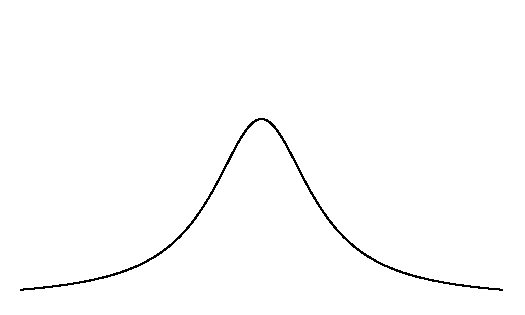
\includegraphics[scale=1.25]{pdfCauchyNB}}
%\date{\vspace{1em}~{}~\\  ~\\ ~{}~\\ \vspace{3em}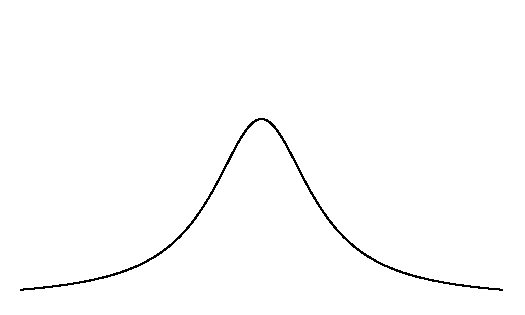
\includegraphics[scale=1.25]{pdfCauchyNB}}
%\date{\vspace{1em}\version\\ ~\\ \number\year}
\maketitle
\thispagestyle{empty}
% \clearpage % BOOK
\thispagestyle{empty}

\iftoggle{formatArticle}{}{\clearpage \thispagestyle{chapter} }
 
~ \vfill


{\center

\version  \\ ~ \\ Copyright \copyright~2010-\number\year~ Gavin E. Crooks
\\
~
\\
ISBN: 978-1-7339381-0-5
~\\~\\
\url{http://threeplusone.com/fieldguide} 
\\
%\url{https://github.com/gecrooks/fieldguide}
%~
%\\
Berkeley Institute for Theoretical Sciences (BITS)
\\
typeset on \isotoday~with XeTeX version  \the\XeTeXversion\XeTeXrevision
\\
fonts: Trump Mediaeval (text), Euler (math)
\\
% 2~7~1~8~2~8~1~8~2~8~4~5~9~0~4~5~2~3~5~3~6~0~2~8~7~4~7~1~3~5~2~7
  2~7~1~8~2~8~1~8~2~8~4~5~9~0~4
\\
~ 
\\

}
%\thispagestyle{empty}
\vspace{3em}

\iftoggle{formatArticle}{\twocolumn}{}	% If article format, reset to two column format


%\vfill
\clearpage



\SecS{Preface: The search for GUD}
\phantomsection\addcontentsline{toc}{section}{Preface: The search for GUD}

A common problem is that of describing the probability distribution of a single, continuous variable. A few distributions, such as the normal and exponential, were discovered in the 1800's or earlier. But about a century ago the great statistician, Karl Pearson, realized that the known probability distributions were not sufficient to handle all of the phenomena then under investigation, and set out to create new distributions with useful properties. 

During the 20th century this process continued with abandon and a vast menagerie of distinct mathematical forms were discovered and invented, investigated, analyzed, rediscovered and renamed, all for the purpose of describing the probability of some interesting variable. There are  hundreds of named distributions and synonyms in current usage. The apparent diversity is unending and disorienting.


Fortunately, the situation is less confused than it might at first appear. Most common, continuous, univariate, unimodal distributions  can be organized into a small number of distinct families, which are all special cases of a single Grand Unified Distribution. This compendium details these hundred or so simple distributions, their properties and their interrelations. 
 ~\\~\\
 \null\hfill~Gavin~E.~Crooks



% !TEX encoding = UTF-8 Unicode 
% !TEX root = FieldGuide.tex


\clearpage

%\thispagestyle{}
%~
%\vspace{18em}
%~
\SecS{Acknowledgments}
\phantomsection\addcontentsline{toc}{section}{Acknowledgments \& Version History} 
%\begin{center}
%\textsc{Acknowledgments}
%\end{center}


In curating this collection of distributions, I have benefited greatly from Johnson, Kotz, and Balakrishnan's monumental compendiums~\cite{Johnson1994, Johnson1995}, Eric Weisstein's MathWorld, the Leemis chart of Univariate Distribution Relationships~\cite{Leemis2008, Leemis2012}, and myriad pseudo-anonymous contributors to Wikipedia. Additional contributions are noted in the version history below.


\begin{center}
\textsc{Version History}
\end{center}

{
\small \tightstretch

0.13 (2019-??-??)
Added
Porter-Thomas \eqref{PorterThomas},
biweight \eqref{Biweight},
triweight \eqref{Triweight},
Johnson~$S_U$ \eqref{JohnsonSU},
and
log-Cauchy \eqref{LogCauchy}
distributions.
% Fixed typos
% Proof checked equations. All renaming errors are figments of your imagination.

~

0.12 (2019-02-14) 
Added
Epanechnikov \eqref{Epanechnikov}, 
Libby-Novick \eqref{LibbyNovick},
Gauss hypergeometric \eqref{GaussHypergeometric},
and
confluent hypergeometric \eqref{Confluent}
distributions. 
% Fixed many typos
% Merged Pearson III and gamma distributions.
% Added figure for log-gamma
% Renamed Prentice to beta-logistic
% Add source control: https://github.com/gecrooks/fieldguide

~

0.11 (2017-06-19)
\sloppy{ Added hyperbola \eqref{Hyperbola}, Halphen \eqref{Halphen}, Halphen B \eqref{HalphenB}, inverse Halphen B \eqref{InvHalphenB}, generalized Halphen \eqref{GenHalphen}, Sichel \eqref{Sichel} and Appell Beta~\eqref{AppellBeta} distributions. Thanks to Saralees Nadarajah.}
% Kudos to Nadarajah for AppellBeta paper.

~

0.10 (2017-02-08)
Added K \eqref{K}  and generalized K  \eqref{GenK} distributions.
% Fixed typos.
% Additional endorsements.
Clarified notation and nomenclature.
Thanks to Harish Vangala.

~

0.9 (2016-10-18)
Added 
	pseudo Voigt \eqref{PseudoVoigt}, 
and
	Student's $t_3$ \eqref{StudentsT3}
distributions.
Reparameterized hyperbolic sine \eqref{HyperbolicSine} distribution.
Renamed inverse Burr to Dagum \eqref{Dagum}. %, and added location scale
Derived limit of unit gamma to log-normal (p\pageref{UnitGammaToLogNormal}). 
Corrected spelling of  ``arrises'' (sharp edges formed by the meeting of surfaces) to ``arises'' (emerge; become apparent). 
% Added figure of limits and reworked limits appendix
% Added figure for order statistics appendix
% Added Endorsements page
% Moved Pearson Exponential to Notes until figure out best organization.
% Removed stretched exponential distribution (Redundant with Weibull)
% Removed Moffat, unclear if correct definition, or if redundant.
% 50% proofed equations

~

0.8 (2016-08-30)
The Unprincipled edition:
Added Moyal distribution \eqref{Moyal}, a special case of the gamma-exponential distribution.
Corrected spelling of ``principle'' to ``principal''. Thanks to Matthew Hankins and Mara Averick.
% Fixed typos and improved formatting.
% Added source control
% Renamed mixture distributions to compound distributions. 
% Added exponential twist, but not done yet.
% Changed all distribution names to links.
% Fixed overfull hboxes

~

0.7 (2016-04-05) 
%
Added Hohlfeld distribution. %and Gauss hypergeometric distributions.
Added appendix on limits.
Reformatted and rationalized distribution hierarchy diagrams. 
%Fixed typos and improved formatting.
Thanks to Phill Geissler.

~

0.6 (2014-12-22)
%
Total of 147 named simple, unimodal, univariate, continuous probability distributions, and at least as many synonyms.
Added appendix on the algebra of random variables.
Added Box-Muller transformation.
For the gamma-exponential distribution, switched the sign on the parameter $\alpha$.
Fixed the relation between beta distributions and ratios of gamma distributions ($\alpha$ and $\gamma$ were switched in most cases).
%Fixed typos and improved formatting.
Thanks to Fabian Kr\"uger and Lawrence Leemis.


~


0.5 (2013-07-01)
Added uniform product, half generalized Pearson VII, half exponential power distributions, GUD and q-Type distributions. 
Moved Pearson IV to own section.
Fixed errors in Inverse Gaussian.
Added random variate generation to appendix.
% Fixed typos. 
Thanks to David Sivak, Dieter Grientschnig, Srividya Iyer-Biswas, and Shervin Fatehi.

~

 0.4 (2012-03-01) 
% Fixed typos.
Added erratics. 
Moved gamma distribution to own section.
Renamed log-gamma to gamma-exponential.
Added permalink.
Added new tree of distributions. 
Thanks to David Sivak and Frederik Beaujean.

~

0.3 (2011-06-40) 
%Fixed many typos.
Added tree of distributions. 
%Improved formatting. 

~

0.2 (2011-03-01) 
%Fixed many typos.
Expanded families.  
Thanks to David Sivak. 

~

 0.1 (2011-01-16)
 Initial release. Organize over 100  simple, continuous, univariate probability distributions into 14 families. Greatly expands on previous paper that discussed the Amoroso and gamma-exponential families~\cite{_amoroso}. Thanks to David Sivak, Edward E. Ayoub, and Francis J. O'Brien.

%~
%0.0 (c2010) Genesis, during a particularly enthralling session of the Berkeley Statistical Mechanics meeting. 
}



\normalstretch
\newpage ~\newpage

\SSecS{Endorsements}
~\\

\noindent
``\emph{Ridiculously useful}'' -- Mara Averick\footnote{\url{https://twitter.com/dataandme/status/770732084872810496}}
\\

\noindent
``\emph{I can't stress how useful I've found this. I wish I'd had a printout of it by my desk every day for the last 6 years}''-- Guillermo Roditi Dominguez\footnote{\url{https://twitter.com/groditi/status/772266190190194688}}
\\

\noindent
``\emph{Abramowitz and Stegun for probability distributions}''-- Kranthi K. Mandadapu\footnote{Thursday Lunch with Scientists}
\\

\noindent
``\emph{I had no idea how much I needed this guide.}''-- Daniel J. Harris\footnote{\url{https://twitter.com/DHarrisPsyc/status/870614354529370112}}
\\



\noindent
``\emph{Who are you? How did you get in my house?}'' -- Donald Knuth\footnote{\url{https://xkcd.com/163/}}
\\




\clearpage
\phantomsection\addcontentsline{toc}{section}{Contents}
\thispagestyle{chapter}
\tableofcontents
\clearpage

% Use short alternative Table and Figure captions to keep one line per
\listoffigures
\phantomsection\addcontentsline{toc}{section}{List of figures}
%\thispagestyle{chapter}
\clearpage % BOOK
%\newpage
%\thispagestyle{chapter}
\phantomsection\addcontentsline{toc}{section}{List of tables}
\listoftables
\clearpage

% ~ \clearpage


% !TEX encoding = UTF-8 Unicode 
% !TEX root = FieldGuide.tex

\clearpage
\thispagestyle{chapter}
\begin{figure*}
\phantomsection\addcontentsline{toc}{section}{Distribution hierarchies} 
\phantomsection\addcontentsline{toc}{subsection}{Hierarchy of principal distributions} 
\caption[Hierarchy of principal distributions]{Hierarchy of principal distributions} 
\label{PrincipalHierarchy}
\begin{center}
\scalebox{0.58} {
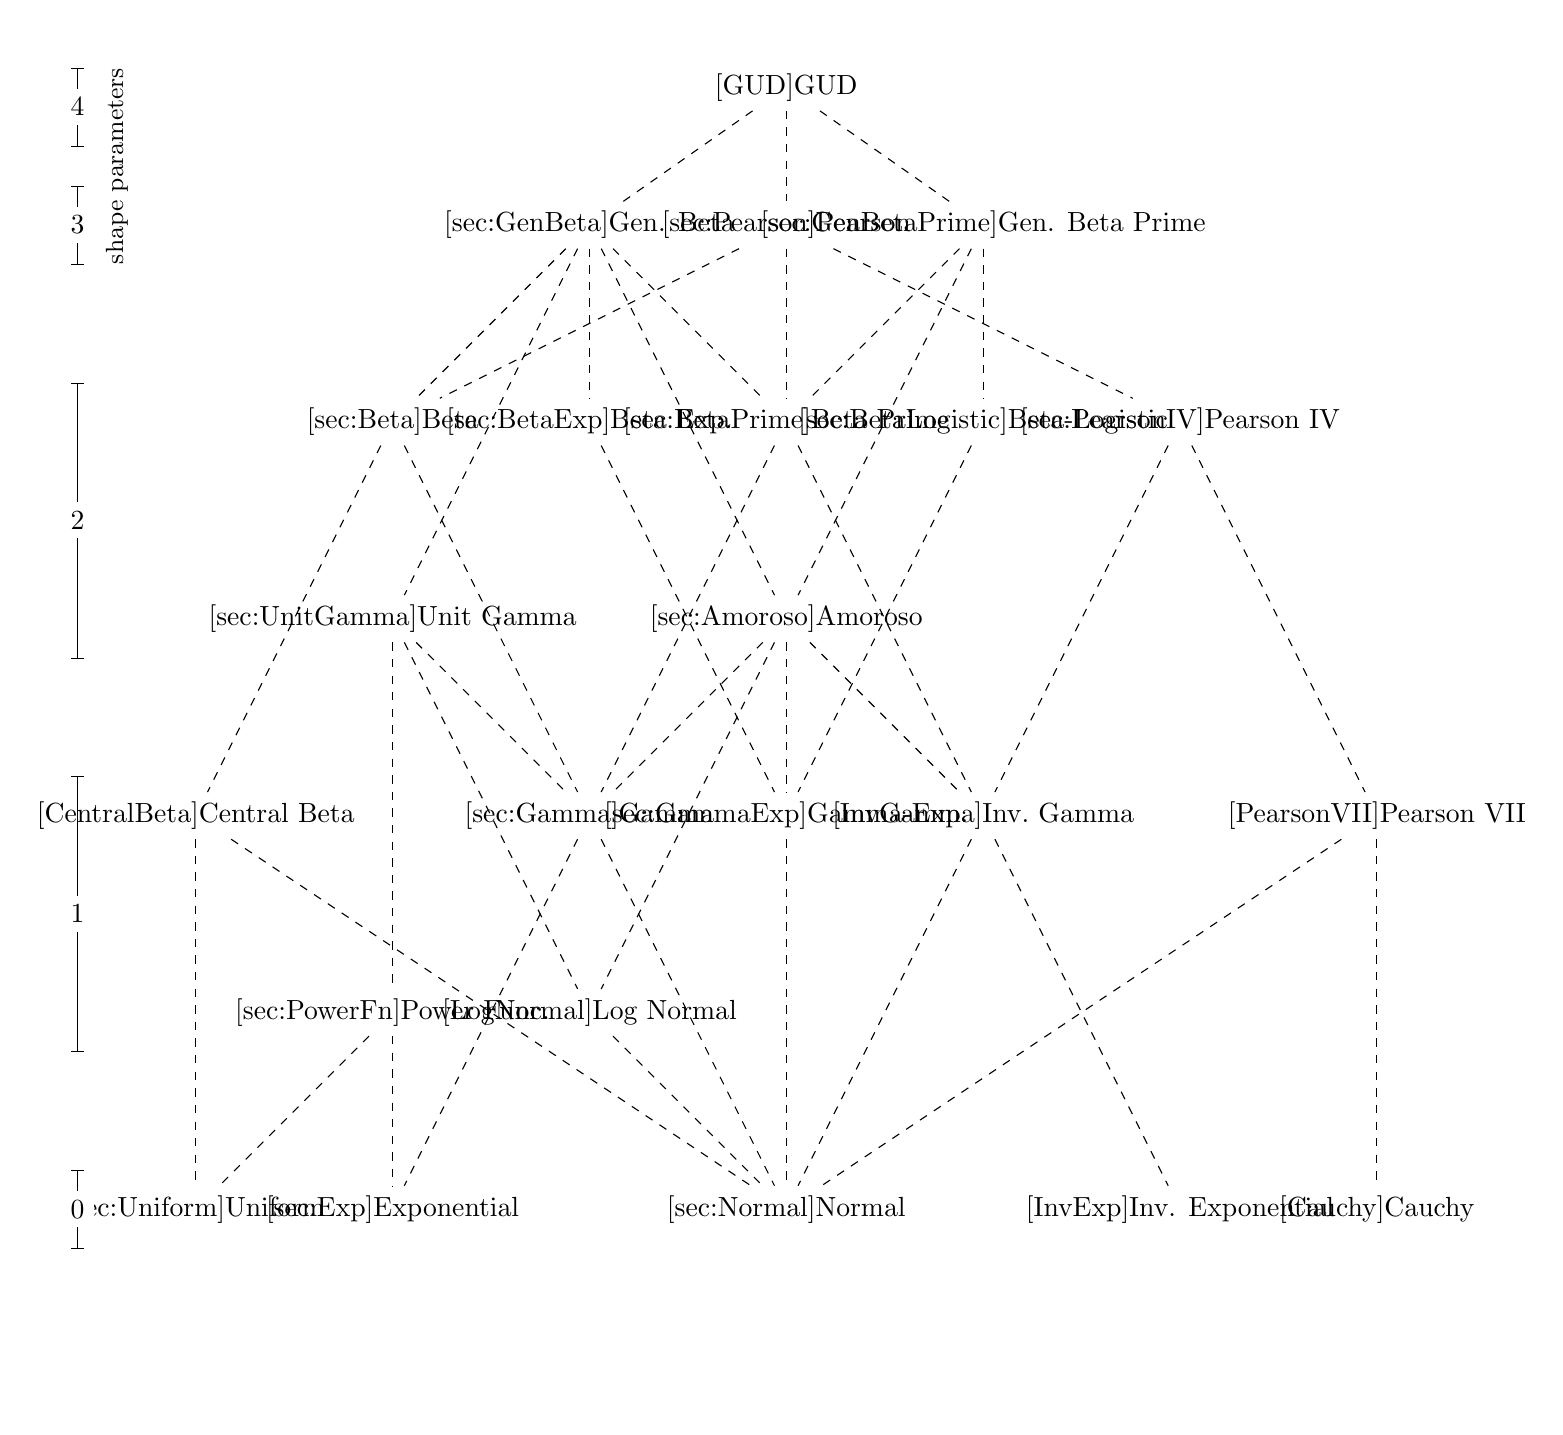
\begin{tikzpicture}
%\draw[help lines, very thin, step=1] (-2,0) grid (17,17);
%
\draw (7.5,16.75) node (gud) {\hyperref[GUD]{GUD}};
%
\draw (5,15) node (genbeta) {\hyperref[sec:GenBeta]{Gen. Beta}};
\draw (7.5,15) node (pearson) {\hyperref[sec:Pearson]{Pearson}};
\draw (10,15) node (genbetaprime) {\hyperref[sec:GenBetaPrime]{Gen. Beta Prime}};
%
\draw (2.5,12.5) node (beta) {\hyperref[sec:Beta]{Beta}};
\draw (5,12.5) node (betaexp) {\hyperref[sec:BetaExp]{Beta Exp.}};
\draw (7.5,12.5) node (betaprime) {\hyperref[sec:BetaPrime]{Beta Prime}};
\draw (10,12.5) node (betalogistic) {\hyperref[sec:BetaLogistic]{Beta-Logistic}};
\draw (12.5,12.5) node (pearsoniv) {\hyperref[sec:PearsonIV]{Pearson IV}};
%
\draw (2.5,10) node (unitgamma) {\hyperref[sec:UnitGamma]{Unit Gamma}};
\draw (7.5,10) node (amoroso) {\hyperref[sec:Amoroso]{Amoroso}};
%\draw (12.5,10) node (burr) {\hyperref[Burr]{Burr}};
%
%\draw (0,7.5) node  (pearsonii) {\hyperref[PearsonII]{Pearson II}};
\draw (0,7.5) node  (pearsonii) {\hyperref[CentralBeta]{Central Beta}};
\draw (2.5,5) node (power)  {\hyperref[sec:PowerFn]{Power Func.}};
\draw (5,7.5) node  (gamma) {\hyperref[sec:Gamma]{Gamma}};
\draw (7.5,7.5) node (gammaexp)  {\hyperref[sec:GammaExp]{Gamma-Exp.}};
\draw (10,7.5) node (invgamma) {\hyperref[InvGamma]{Inv.~Gamma}}; 
%\draw (12.5,7.5) node  (loglogistic) {\hyperref[LogLogistic]{Log-Logistic}};
\draw (15,7.5) node (pearsonvii) {\hyperref[PearsonVII]{Pearson VII }};
%
%\draw (10,7.5) node (symbetalogistic) [text width=3cm, align=center] {\hyperref[CentralLogistic]{Central-Logistic}};

%\draw (5,5) node (weibull) {\hyperref[Weibull]{Weibull}};
%\draw (7.5,5) node (symbetalogistic) {\hyperref[SymBetaLogistic]{Sym. Beta-Logistic}};
%\draw (10,5) node (frechet) {\hyperref[Frechet]{Frechet}};
%\draw (12.5,7.5) node (lognormal) {\hyperref[LogNormal]{Log Normal}};
\draw (5,5) node (lognormal) {\hyperref[LogNormal]{Log Normal}};
%
\draw (0,2.5) node (uniform) {\hyperref[sec:Uniform]{Uniform}};
\draw (2.5,2.5) node (exp) {\hyperref[sec:Exp]{Exponential}};
%\draw (5,2.5) node (laplace) {\hyperref[sec:Laplace]{Laplace}};
\draw (7.5,2.5) node (normal) {\hyperref[sec:Normal]{Normal}};
%\draw (10,2.5) node (UniPrime) {\hyperref[Logistic]{Uniform Prime}};
%\draw (10,2.5) node (logistic) {\hyperref[Logistic]{Logistic}};
\draw (12.5,2.5) node (invexp) {\hyperref[InvExp]{Inv. Exponential}};
\draw (15,2.5) node (cauchy) {\hyperref[Cauchy]{Cauchy}};
%
%\draw (7.5,0) node (gumbel) {\hyperref[Gumbel]{Gumbel}};
%
\draw [dashed]  (gud) -- (genbeta);
\draw [dashed]  (gud) -- (pearson);
\draw [dashed]  (gud) -- (genbetaprime);
%
\def\betaone{node}%
\draw [dashed]  (genbeta) --  (beta);
\draw [dashed]  (genbeta) --  (betaexp);
\draw [dashed]  (genbeta) --  (betaprime);
\draw [dashed]  (genbeta) -- (unitgamma);
\draw [dashed]  (genbeta) -- (amoroso);
%
\draw [dashed]  (pearson) -- (beta);
\draw [dashed]  (pearson) -- (betaprime);
\draw [dashed]  (pearson) -- (pearsoniv);
%
\draw [dashed]  (genbetaprime) -- (betalogistic);
\draw [dashed]  (genbetaprime) -- (betaprime);
\draw [dashed]  (genbetaprime) -- (amoroso);
%\draw [dashed]  (genbetaprime) -- (burr);
%
\draw [dashed]  (beta) -- (pearsonii);
\draw [dashed]  (beta) -- (gamma);
%
\draw [dashed]  (betaexp) -- (gammaexp);
%
\draw [dashed]  (betaprime) -- (gamma);
\draw [dashed]  (betaprime) -- (invgamma);
%
\draw [dashed]  (betalogistic) -- (gammaexp);
%\draw [dashed]  (betalogistic) -- (symbetalogistic);
%
\draw [dashed]  (pearsoniv) -- (invgamma);
\draw [dashed]  (pearsoniv) -- (pearsonvii);
\draw [dashed] (unitgamma) -- (power);
\draw [dashed]  (unitgamma) -- (gamma);
%
\draw [dashed]  (amoroso) -- (gamma);
%\draw [dashed]  (amoroso) -- (weibull);
\draw [dashed]  (amoroso) -- (gammaexp);
\draw [dashed]  (amoroso) -- (invgamma);
%\draw [dashed]  (amoroso) -- (frechet);
%
%\draw [dashed]  (burr) -- (frechet);
%\draw [dashed]  (burr) -- (loglogistic);
%
\draw [dashed]  (pearsonii) -- (uniform);
\draw [dashed]  (pearsonii) -- (normal);
\draw [dashed]  (power) -- (uniform);
\draw [dashed]  (power) -- (exp);
\draw [dashed]  (gamma) -- (exp);
\draw [dashed]  (gamma) -- (normal);
\draw [dashed]  (invgamma) -- (normal);
\draw [dashed]  (invgamma) -- (invexp);
%\draw [dashed]  (loglogistic) -- (logistic);
\draw [dashed]  (pearsonvii) -- (normal);
\draw [dashed]  (pearsonvii) -- (cauchy);
%
%\draw [dashed]  (weibull) -- (exp);
%\draw [dashed]  (weibull) -- (gumbel);
%\draw [dashed]  (symbetalogistic) -- (laplace);
%\draw [dashed]  (symbetalogistic) -- (normal);
%\draw [dashed]  (symbetalogistic) -- (logistic);
%\draw [dashed]  (frechet) -- (gumbel);
%\draw [dashed]  (frechet) -- (invexp);
\draw [dashed] (amoroso) -- (lognormal);
\draw [dashed] (unitgamma) -- (lognormal);		
\draw [dashed] (lognormal) -- (normal);
%
%\draw [dashed] (amoroso) -- +(5, -1.5)-- (lognormal);
%\draw [dashed] (gammaexp) -- +(0,-1) ;
%\draw [dashed] (gumbel) -- +(0,0.75) ;
%\draw [dashed] (gammaexp)  -- (gumbel) ;
\draw [dashed] (gammaexp)  -- (normal) ;
%
%\draw (7.5,7.5) node[fill=white, fill opacity=0.75] {\hyperref[sec:GammaExp]{Gamma-Exp.}};
%\draw (7.5,5) node[fill=white, fill opacity=0.75] {\hyperref[SymBetaLogistic]{Sym. Beta-Logistic}};
%
\draw[|-|, very thin] (-1.5,2) -- node[fill=white, midway] {0} (-1.5,3);
\draw[|-|, very thin]  (-1.5,4.5) -- node[fill=white, midway] {1} (-1.5,8);
\draw[|-|, very thin]  (-1.5,9.5) -- node[fill=white, midway] {2} (-1.5,13);
\draw[|-|, very thin]  (-1.5,14.5) -- node[fill=white, midway] {3} (-1.5,15.5);
\draw[|-|, very thin]  (-1.5,16) -- node[fill=white, midway] {4} (-1.5,17);
%
\draw (-1, 15.75) node[rotate=90]  {\small shape parameters};
%
\draw[white] (-2, 0) rectangle (17,17.5); % Bounding box
\end{tikzpicture}
}
\end{center}
\end{figure*}



% !TEX encoding = UTF-8 Unicode 
% !TEX root = FieldGuide.tex

\clearpage
\thispagestyle{chapter}
\begin{figure*}
\phantomsection\addcontentsline{toc}{subsection}{Hierarchy of Pearson distributions} 
\caption{Hierarchy of Pearson distributions } 
\label{PearsonHierarchy}
\begin{center}
\scalebox{0.58} {
\begin{tikzpicture}
%\draw[help lines, very thin, step=1] (-2,0) grid (17,17);
%
%\draw (7.5,16.75) node (gud) {\hyperref[GUD]{GUD}};
%
%\draw (5,15) node (genbeta) {\hyperref[sec:GenBeta]{Gen. Beta}};
\draw (7.5,15) node (pearson) {\hyperref[sec:Pearson]{Pearson}};
%\draw (10,15) node (genbetaprime) {\hyperref[sec:GenBetaPrime]{Gen. Beta Prime}};
%
\draw (2.5,12.5) node (beta) {\hyperref[sec:Beta]{Beta}};
%\draw (5,12.5) node (betaexp) {\hyperref[sec:BetaExp]{Beta Exp.}};
\draw (7.5,12.5) node (betaprime) {\hyperref[sec:BetaPrime]{Beta Prime}};
\draw (12.5,12.5) node (pearsoniv) {\hyperref[sec:PearsonIV]{Pearson IV}};
%
%\draw (2.5,10) node (unitgamma) {\hyperref[sec:UnitGamma]{Unit Gamma}};
%\draw (7.5,10) node (amoroso) {\hyperref[sec:Amoroso]{Amoroso}};
%\draw (12.5,10) node (burr) {\hyperref[Burr]{Burr}};
%
\draw (0,7.5) node  (pearsonii) {\hyperref[CentralBeta]{Central Beta}};
%\draw (2.5,7.5) node (power)  {\hyperref[sec:PowerFn]{Power Func.}};
\draw (5,7.5) node  (gamma) {\hyperref[sec:Gamma]{Gamma}};
%\draw (7.5,7.5) node (gammaexp)  {\hyperref[sec:GammaExp]{Gamma-Exp.}};
\draw (10,7.5) node (invgamma) {\hyperref[InvGamma]{Inv.~Gamma}}; 
%\draw (12.5,7.5) node  (loglogistic) {\hyperref[LogLogistic]{Log-Logistic}};
\draw (15,7.5) node (pearsonvii) {\hyperref[PearsonVII]{Pearson VII }};
%
%\draw (5,5) node (weibull) {\hyperref[Weibull]{Weibull}};
%\draw (10,5) node (frechet) {\hyperref[Frechet]{Frechet}};
%\draw (13.75,5) node (lognormal) {\hyperref[LogNormal]{Log Normal}};
%
\draw (0,2.5) node (uniform) {\hyperref[sec:Uniform]{Uniform}};
\draw (2.5,2.5) node (exp) {\hyperref[sec:Exp]{Exponential}};
%\draw (5,2.5) node (laplace) {\hyperref[sec:Laplace]{Laplace}};
\draw (7.5,2.5) node (normal) {\hyperref[sec:Normal]{Normal}};
%\draw (10,2.5) node (logistic) {\hyperref[Logistic]{Logistic}};
\draw (12.5,2.5) node (invexp) {\hyperref[InvExp]{Inv. Exponential}};
\draw (15,2.5) node (cauchy) {\hyperref[Cauchy]{Cauchy}};
%
%\draw (7.5,1) node (gumbel) {\hyperref[Gumbel]{Gumbel}};
%
%\draw [dashed]  (gud) -- (genbeta);
%\draw [dashed]  (gud) -- (pearson);
%\draw [dashed]  (gud) -- (genbetaprime);
%
%\draw [dashed]  (genbeta) -- (beta);
%\draw [dashed]  (genbeta) -- (betaexp);
%\draw [dashed]  (genbeta) -- (betaprime);
%\draw [dashed]  (genbeta) -- (unitgamma);
%\draw [dashed]  (genbeta) -- (amoroso);
%
\draw [dashed]  (pearson) -- (beta);
\draw [dashed]  (pearson) -- (betaprime);
\draw [dashed]  (pearson) -- (pearsoniv);
%
%\draw [dashed]  (genbetaprime) -- (betaprime);
%\draw [dashed]  (genbetaprime) -- (amoroso);
%\draw [dashed]  (genbetaprime) -- (burr);
%
\draw [dashed]  (beta) -- (pearsonii);
\draw [dashed]  (beta) -- (gamma);
%
%\draw [dashed]  (betaexp) -- (gammaexp);
%
\draw [dashed]  (betaprime) -- (gamma);
\draw [dashed]  (betaprime) -- (invgamma);
%
%
\draw [dashed]  (pearsoniv) -- (invgamma);
\draw [dashed]  (pearsoniv) -- (pearsonvii);
%\draw [dashed] (unitgamma) -- (power);
%\draw [dashed]  (unitgamma) -- (gamma);
%
%\draw [dashed]  (amoroso) -- (gamma);
%\draw [dashed]  (amoroso) -- (weibull);
%\draw [dashed]  (amoroso) -- (gammaexp);
%\draw [dashed]  (amoroso) -- (invgamma);
%\draw [dashed]  (amoroso) -- (frechet);
%
%\draw [dashed]  (burr) -- (frechet);
%\draw [dashed]  (burr) -- (loglogistic);
%
\draw [dashed]  (pearsonii) -- (uniform);
\draw [dashed]  (pearsonii) -- (normal);
%\draw [dashed]  (power) -- (uniform);
%\draw [dashed]  (power) -- (exp);
\draw [dashed]  (gamma) -- (exp);
\draw [dashed]  (gamma) -- (normal);
\draw [dashed]  (invgamma) -- (normal);
\draw [dashed]  (invgamma) -- (invexp);
%\draw [dashed]  (loglogistic) -- (logistic);
\draw [dashed]  (pearsonvii) -- (normal);
\draw [dashed]  (pearsonvii) -- (cauchy);
%
%\draw [dashed]  (weibull) -- (exp);
%\draw [dashed]  (weibull) -- (gumbel);
%\draw [dashed]  (frechet) -- (gumbel);
%\draw [dashed]  (frechet) -- (invexp);
%\draw [dashed] (lognormal) -- (normal);
%
%\draw [dashed] (amoroso) -- +(6.25, -1.5)-- (lognormal);
%\draw [dashed] (gammaexp) -- +(0,-1) ;
%\draw [dashed] (gumbel) -- +(0,0.75) ;
%
%\draw (7.5,7.5) node[fill=white, fill opacity=0.75] {Gamma-Exp.};
%
\draw[|-|, very thin] (-1.5,2) -- node[fill=white, midway] {0} (-1.5,3);
\draw[|-|, very thin]  (-1.5,4.5) -- node[fill=white, midway] {1} (-1.5,8);
\draw[|-|, very thin]  (-1.5,9.5) -- node[fill=white, midway] {2} (-1.5,13);
\draw[|-|, very thin]  (-1.5,14.5) -- node[fill=white, midway] {3} (-1.5,15.5);
\draw[|-|, very thin]  (-1.5,16) -- node[fill=white, midway] {4} (-1.5,17);
%
\draw (-1, 15.75) node[rotate=90]  {\small shape parameters};
%
\draw[white] (-2, 0) rectangle (17,17.5); % Bounding box
\end{tikzpicture}
}

\end{center}
\end{figure*}

% !TEX encoding = UTF-8 Unicode 
% !TEX root = FieldGuide.tex

\clearpage
\thispagestyle{chapter}
\begin{figure*}
\phantomsection\addcontentsline{toc}{subsection}{Hierarchy of Pearson-exponential distributions} 
\caption[Hierarchy of Pearson-exponential distributions]{Hierarchy of Pearson-exponential distributions} 
\label{PearsonExpHierarchy}
\begin{center}
\scalebox{0.58} {
\begin{tikzpicture}
%\draw[help lines, very thin, step=1] (-2,0) grid (17,17);
%
%\draw (7.5,16.75) node (gud) {\hyperref[GUD]{GUD}};
%
%\draw (5,15) node (genbeta) {\hyperref[sec:GenBeta]{Gen. Beta}};
\draw (7.5,15) node (pearsonexp) {\hyperref[PearsonExp]{Pearson-Exp.}};
%\draw (10,15) node (genbetaprime) {\hyperref[sec:GenBetaPrime]{Gen. Beta Prime}};
%
%\draw (2.5,12.5) node (beta) {\hyperref[sec:Beta]{Beta}};
\draw (5,12.5) node (betaexp) {\hyperref[sec:BetaExp]{Beta-Exp.}};
%\draw (7.5,12.5) node (betaprime) {\hyperref[sec:BetaPrime]{Beta Prime}};
\draw (10,12.5) node (betalogistic) {\hyperref[sec:BetaLogistic]{Beta-Logistic}};
%\draw (12.5,12.5) node (pearsoniv) {\hyperref[sec:PearsonIV]{Pearson IV}};
%
%\draw (2.5,10) node (unitgamma) {\hyperref[sec:UnitGamma]{Unit Gamma}};
%\draw (7.5,10) node (amoroso) {\hyperref[sec:Amoroso]{Amoroso}};
%\draw (12.5,10) node (burr) {\hyperref[Burr]{Burr}};
%
%\draw (0,7.5) node  (pearsonii) {\hyperref[PearsonII]{Pearson II}};
%\draw (2.5,5) node (power)  {\hyperref[sec:PowerFn]{Power Func.}};
%\draw (5,7.5) node  (gamma) {\hyperref[sec:Gamma]{Gamma}};
\draw (2.5,7.5) node (expexp) [text width=3cm, align=center] {\hyperref[ExpExp]{Exp.\ Exponential}};
\draw (7.5,7.5) node (gammaexp)  {\hyperref[sec:GammaExp]{Gamma-Exp.}};
\draw (12.5,7.5) node (burrii)  {\hyperref[BurrII]{Burr II}};
\draw (10,7.5) node (symbetalogistic) [text width=3cm, align=center] {\hyperref[CentralLogistic]{Central-Logistic}};

%\draw (10,7.5) node (invgamma) {\hyperref[InvGamma]{Inv. gamma}}; 
%\draw (12.5,7.5) node  (loglogistic) {\hyperref[LogLogistic]{Log-Logistic}};
%\draw (15,7.5) node (pearsonvii) {\hyperref[PearsonVII]{Pearson VII }};
%
%\draw (5,5) node (weibull) {\hyperref[Weibull]{Weibull}};
%\draw (7.5,5) node (symbetalogistic) {\hyperref[SymBetaLogistic]{Sym. Beta-Logistic}};
%\draw (10,5) node (frechet) {\hyperref[Frechet]{Frechet}};
%\draw (12.5,7.5) node (lognormal) {\hyperref[LogNormal]{Log Normal}};
%\draw (5,5) node (lognormal) {\hyperref[LogNormal]{Log Normal}};
%
%\draw (0,2.5) node (uniform) {\hyperref[sec:Uniform]{Uniform}};
\draw (2.5,2.5) node (exp) {\hyperref[sec:Exp]{Exponential}};
\draw (10,2.5) node (laplace) {\hyperref[sec:Laplace]{Laplace}};
\draw (7.5,2.5) node (gumbel) {\hyperref[Gumbel]{Gumbel}};
%\draw (10,2.5) node (UniPrime) {\hyperref[Logistic]{Uniform Prime}};
\draw (12.5,2.5) node (logistic) {\hyperref[Logistic]{Logistic}};
%\draw (12.5,2.5) node (invexp) {\hyperref[InvExp]{Inv. Exponential}};
%\draw (15,2.5) node (cauchy) {\hyperref[Cauchy]{Cauchy}};
%
%t\draw (7.5,0) node (gumbel) {\hyperref[Gumbel]{Gumbel}};
%
%\draw [dashed]  (gud) -- (genbeta);
%\draw [dashed]  (gud) -- (pearson);
%\draw [dashed]  (gud) -- (genbetaprime);
%
\def\betaone{node}%
%\draw [dashed]  (genbeta) --  (beta);
%\draw [dashed]  (genbeta) --  (betaexp);
%\draw [dashed]  (genbeta) --  (betaprime);
%\draw [dashed]  (genbeta) -- (unitgamma);
%\draw [dashed]  (genbeta) -- (amoroso);
%
\draw [dashed]  (pearsonexp) -- (betaexp);
\draw [dashed]  (pearsonexp) -- (betalogistic);
%\draw [dashed]  (pearson) -- (pearsoniv);
%
%\draw [dashed]  (genbetaprime) -- (betalogistic);
%\draw [dashed]  (genbetaprime) -- (betaprime);
%\draw [dashed]  (genbetaprime) -- (amoroso);
%\draw [dashed]  (genbetaprime) -- (burr);
%
%\draw [dashed]  (beta) -- (pearsonii);
%\draw [dashed]  (beta) -- (gamma);
%
\draw [dashed]  (betaexp) -- (gammaexp);
%
%\draw [dashed]  (betaprime) -- (gamma);
%\draw [dashed]  (betaprime) -- (invgamma);
%
\draw [dashed]  (betalogistic) -- (gammaexp);
\draw [dashed]  (symbetalogistic) -- (laplace);
\draw [dashed]  (symbetalogistic) -- (logistic);
\draw [dashed]  (betalogistic) -- (symbetalogistic);
\draw [dashed]  (expexp) -- (gumbel);				% TODO: Checkme

%
%
%\draw [dashed]  (weibull) -- (exp);
%\draw [dashed]  (weibull) -- (gumbel);
%\draw [dashed]  (symbetalogistic) -- (laplace);
%\draw [dashed]  (symbetalogistic) -- (normal);
%\draw [dashed]  (symbetalogistic) -- (logistic);
%\draw [dashed]  (frechet) -- (gumbel);
%\draw [dashed]  (frechet) -- (invexp);
%\draw [dashed] (amoroso) -- (lognormal);
%\draw [dashed] (unitgamma) -- (lognormal);		
%\draw [dashed] (lognormal) -- (normal);
%
%\draw [dashed] (amoroso) -- +(5, -1.5)-- (lognormal);
%\draw [dashed] (gammaexp) -- +(0,-1) ;
%\draw [dashed] (gumbel) -- +(0,0.75) ;
\draw [dashed] (gammaexp)  -- (gumbel) ;
\draw [dashed] (betalogistic)  -- (burrii) ;
\draw [dashed] (burrii)  -- (logistic) ;
\draw [dashed] (betaexp)  -- (expexp) ;
\draw [dashed] (expexp)  -- (exp) ;
\draw [dashed] (burrii)  -- (gumbel) ;

%\draw [dashed] (gammaexp)  -- (normal) ;
%
\draw (7.5,7.5) node[fill=white, fill opacity=0.75] {\hyperref[sec:GammaExp]{Gamma-Exp.}};
%\draw (7.5,5) node[fill=white, fill opacity=0.75] {\hyperref[SymBetaLogistic]{Sym.\\Beta-Logistic}};
%
\draw[|-|, very thin] (-1.5,2) -- node[fill=white, midway] {0} (-1.5,3);
\draw[|-|, very thin]  (-1.5,4.5) -- node[fill=white, midway] {1} (-1.5,8);
\draw[|-|, very thin]  (-1.5,9.5) -- node[fill=white, midway] {2} (-1.5,13);
\draw[|-|, very thin]  (-1.5,14.5) -- node[fill=white, midway] {3} (-1.5,15.5);
\draw[|-|, very thin]  (-1.5,16) -- node[fill=white, midway] {4} (-1.5,17);
%
\draw (-1, 15.75) node[rotate=90]  {\small shape parameters};
%
\draw[white] (-2, 0) rectangle (17,17.5); % Bounding box
\end{tikzpicture}
}
\end{center}
\end{figure*}



% !TEX encoding = UTF-8 Unicode 
% !TEX root = FieldGuide.tex

\clearpage
\thispagestyle{chapter}
\begin{figure*}
\phantomsection\addcontentsline{toc}{subsection}{Hierarchy of extreme order statistics} 
\caption{Hierarchy of extreme order statistics} 
\begin{center}
\scalebox{0.58} {
\begin{tikzpicture}
%\draw[help lines, very thin, step=1] (-2,0) grid (17,17);
%
\draw (5,5) node (weibull) {\hyperref[Weibull]{Weibull}};
\draw (10,5) node (frechet) {\hyperref[Frechet]{Frechet}};
%\draw (13.75,5) node (lognormal) {\hyperref[LogNormal]{Log Normal}};
%
%\draw (0,2.5) node (uniform) {\hyperref[sec:Uniform]{Uniform}};
\draw (2.5,2.5) node (exp) {\hyperref[sec:Exp]{Exponential}};
%\draw (5,2.5) node (laplace) {\hyperref[sec:Laplace]{Laplace}};
%\draw (7.5,2.5) node (normal) {\hyperref[sec:Normal]{Normal}};
%%\draw (10,2.5) node (logistic) {\hyperref[Logistic]{Logistic}};
\draw (12.5,2.5) node (invexp) {\hyperref[InvExp]{Inv. Exponential}};
%\draw (15,2.5) node (cauchy) {\hyperref[Cauchy]{Cauchy}};
%
\draw (7.5,2.5) node (gumbel) {\hyperref[Gumbel]{Gumbel}};
%
\draw [dashed]  (weibull) -- (exp);
\draw [dashed]  (weibull) -- (gumbel);
\draw [dashed]  (frechet) -- (gumbel);
\draw [dashed]  (frechet) -- (invexp);
%
\draw[|-|, very thin] (-1.5,2) -- node[fill=white, midway] {0} (-1.5,3);
\draw[|-|, very thin]  (-1.5,4.5) -- node[fill=white, midway] {1} (-1.5,8);
\draw[|-|, very thin]  (-1.5,8.5) -- node[fill=white, midway] {2} (-1.5,13);
\draw[|-|, very thin]  (-1.5,14.5) -- node[fill=white, midway] {3} (-1.5,15.5);
\draw[|-|, very thin]  (-1.5,16) -- node[fill=white, midway] {4} (-1.5,17);
%
\draw (-1, 15.75) node[rotate=90]  {\small shape parameters};
%
\draw[white] (-2, 0) rectangle (17,17.5); % Bounding box
%
\draw (5,8.75) node (GenWeibull) {\hyperref[GenWeibull]{Gen. Weibull}};
\draw (7.5,10) node (GenFisherTippett) {\hyperref[GenFisherTippett]{Gen. Fisher-Tippett}};
\draw (10,8.75) node (GenFrechet) {\hyperref[GenFrechet]{Gen. Frechet}};
\draw (7.5,7.5) node (FisherTippett) {\hyperref[FisherTippett]{Fisher-Tippett}};
\draw (7.5,5) node (GenGumbel) {\hyperref[GenGumbel]{Gen. Gumbel}};
%
\draw [dashed]  (GenFisherTippett) -- (GenWeibull);
\draw [dashed]  (GenFisherTippett) -- (FisherTippett);
\draw [dashed]  (GenFisherTippett) -- (GenFrechet);
\draw [dashed]  (GenWeibull) -- (weibull);
\draw [dashed]  (GenWeibull) -- (GenGumbel);
\draw [dashed]  (FisherTippett) -- (weibull);
\draw [dashed]  (FisherTippett) -- (frechet);
\draw [dashed]  (GenFrechet) -- (GenGumbel);
\draw [dashed]  (GenFrechet) -- (frechet);
\draw [dashed]  (GenGumbel) -- (gumbel);
\end{tikzpicture}
}
\end{center}
\end{figure*}


\clearpage
\thispagestyle{chapter}
\begin{figure*}
\phantomsection\addcontentsline{toc}{subsection}{Symmetric simple distributions} 
\caption{Hierarchies of symmetric simple distributions} 
\label{SymmetricHierarchy}\begin{center}
\scalebox{0.58} {
\begin{tikzpicture}
%\draw[help lines, very thin, step=1] (-2,0) grid (17,17);
%
%\draw (7.5,16.75) node (gud) {\hyperref[GUD]{GUD}};
%
%\draw (5,15) node (genbeta) {\hyperref[sec:GenBeta]{Gen. Beta}};
%\draw (7.5,15) node (pearson) {\hyperref[sec:Pearson]{Pearson}};
%\draw (10,15) node (genbetaprime) {\hyperref[sec:GenBetaPrime]{Gen. Beta Prime}};
%
%\draw (2.5,12.5) node (beta) {\hyperref[sec:Beta]{Beta}};
%\draw (5,12.5) node (betaexp) {\hyperref[sec:BetaExp]{Beta Exp.}};
%\draw (7.5,12.5) node (betaprime) {\hyperref[sec:BetaPrime]{Beta Prime}};
%\draw (12.5,12.5) node (pearsoniv) {\hyperref[sec:PearsonIV]{Pearson IV}};
%
%\draw (2.5,10) node (unitgamma) {\hyperref[sec:UnitGamma]{Unit Gamma}};
%\draw (7.5,10) node (amoroso) {\hyperref[sec:Amoroso]{Amoroso}};
%\draw (12.5,10) node (burr) {\hyperref[Burr]{Burr}};
%
\draw (0,7.5) node  (pearsonii) {\hyperref[PearsonII]{Pearson II}};
%\draw (2.5,7.5) node (power)  {\hyperref[sec:PowerFn]{Power Func.}};
%\draw (5,7.5) node  (gamma) {\hyperref[sec:Gamma]{Gamma}};
%\draw (7.5,7.5) node (gammaexp)  {\hyperref[sec:GammaExp]{Gamma-Exp.}};
%\draw (10,7.5) node (invgamma) {\hyperref[InvGamma]{Inv. gamma}}; 
%\draw (12.5,7.5) node  (loglogistic) {\hyperref[LogLogistic]{Log-Logistic}};
\draw (15,7.5) node (pearsonvii) {\hyperref[PearsonVII]{Pearson VII }};
%
%\draw (5,5) node (weibull) {\hyperref[Weibull]{Weibull}};
\draw (10,7.5) node (symbetalogistic) {\hyperref[SymBetaLogistic]{Sym. Beta-Logistic}};
%\draw (10,5) node (frechet) {\hyperref[Frechet]{Frechet}};
%\draw (13.75,5) node (lognormal) {\hyperref[LogNormal]{Log Normal}};
%
\draw (0,2.5) node (uniform) {\hyperref[sec:Uniform]{Uniform}};
%\draw (2.5,2.5) node (exp) {\hyperref[sec:Exp]{Exponential}};
\draw (10,2.5) node (laplace) {\hyperref[sec:Laplace]{Laplace}};
\draw (7.5,2.5) node (normal) {\hyperref[sec:Normal]{Normal}};
\draw (12.5,2.5) node (logistic) {\hyperref[Logistic]{Logistic}};
%\draw (12.5,2.5) node (invexp) {\hyperref[InvExp]{Inv. Exponential}};
\draw (15,2.5) node (cauchy) {\hyperref[Cauchy]{Cauchy}};
%
%\draw (7.5,1) node (gumbel) {\hyperref[Gumbel]{Gumbel}};
%
%\draw [dashed]  (gud) -- (genbeta);
%\draw [dashed]  (gud) -- (pearson);
%\draw [dashed]  (gud) -- (genbetaprime);
%
%\draw [dashed]  (genbeta) -- (beta);
%\draw [dashed]  (genbeta) -- (betaexp);
%\draw [dashed]  (genbeta) -- (betaprime);
%\draw [dashed]  (genbeta) -- (unitgamma);
%\draw [dashed]  (genbeta) -- (amoroso);
%
%\draw [dashed]  (pearson) -- (beta);
%\draw [dashed]  (pearson) -- (betaprime);
%\draw [dashed]  (pearson) -- (pearsoniv);
%
%\draw [dashed]  (genbetaprime) -- (betalogistic);
%\draw [dashed]  (genbetaprime) -- (betaprime);
%\draw [dashed]  (genbetaprime) -- (amoroso);
%\draw [dashed]  (genbetaprime) -- (burr);
%
%\draw [dashed]  (beta) -- (pearsonii);
%\draw [dashed]  (beta) -- (gamma);
%
%\draw [dashed]  (betaexp) -- (gammaexp);
%
%\draw [dashed]  (betaprime) -- (gamma);
%\draw [dashed]  (betaprime) -- (invgamma);
%
%\draw [dashed]  (betalogistic) -- (gammaexp);
%\draw [dashed]  (betalogistic) -- (symbetalogistic);
%
%\draw [dashed]  (pearsoniv) -- (invgamma);
%\draw [dashed]  (pearsoniv) -- (pearsonvii);
%\draw [dashed] (unitgamma) -- (power);
%\draw [dashed]  (unitgamma) -- (gamma);
%
%\draw [dashed]  (amoroso) -- (gamma);
%\draw [dashed]  (amoroso) -- (weibull);
%\draw [dashed]  (amoroso) -- (gammaexp);
%\draw [dashed]  (amoroso) -- (invgamma);
%\draw [dashed]  (amoroso) -- (frechet);
%
%\draw [dashed]  (burr) -- (frechet);
%\draw [dashed]  (burr) -- (loglogistic);
%
\draw [dashed]  (pearsonii) -- (uniform);
\draw [dashed]  (pearsonii) -- (normal);
%\draw [dashed]  (power) -- (uniform);
%\draw [dashed]  (power) -- (exp);
%\draw [dashed]  (gamma) -- (exp);
%\draw [dashed]  (gamma) -- (normal);
%\draw [dashed]  (invgamma) -- (normal);
%\draw [dashed]  (invgamma) -- (invexp);
%\draw [dashed]  (loglogistic) -- (logistic);
\draw [dashed]  (pearsonvii) -- (normal);
\draw [dashed]  (pearsonvii) -- (cauchy);
%
%\draw [dashed]  (weibull) -- (exp);
%\draw [dashed]  (weibull) -- (gumbel);
\draw [dashed]  (symbetalogistic) -- (laplace);
\draw [dashed]  (symbetalogistic) -- (normal);
\draw [dashed]  (symbetalogistic) -- (logistic);
%\draw [dashed]  (frechet) -- (gumbel);
%\draw [dashed]  (frechet) -- (invexp);
%\draw [dashed] (lognormal) -- (normal);
%
%\draw [dashed] (amoroso) -- +(6.25, -1.5)-- (lognormal);
%\draw [dashed] (gammaexp) -- +(0,-1) ;
%\draw [dashed] (gumbel) -- +(0,0.75) ;
%
%\draw (7.5,7.5) node[fill=white, fill opacity=0.75] {Gamma-Exp.};
%\draw (7.5,5) node[fill=white, fill opacity=0.75] {Sym. Beta-Logistic};
%
\draw[|-|, very thin] (-1.5,0.5) -- node[fill=white, midway] {0} (-1.5,3);
\draw[|-|, very thin]  (-1.5,4.5) -- node[fill=white, midway] {1} (-1.5,8);
\draw[|-|, very thin]  (-1.5,9.5) -- node[fill=white, midway] {2} (-1.5,13);
\draw[|-|, very thin]  (-1.5,14.5) -- node[fill=white, midway] {3} (-1.5,15.5);
\draw[|-|, very thin]  (-1.5,16) -- node[fill=white, midway] {4} (-1.5,17);
%
\draw (-1, 15.75) node[rotate=90]  {\small shape parameters};
%
\draw[white] (-2, 0) rectangle (17,17.5); % Bounding box
%
\draw (7.5,10) node (QGaussian) {\hyperref[QGaussian]{q-Gaussian}};
\draw [dashed]  (QGaussian) -- (pearsonii);
\draw [dashed]  (QGaussian) -- (pearsonvii);
\end{tikzpicture}
}
\end{center}
\end{figure*}



% ====================================================================

% Zero shape parameters

% !TEX encoding = UTF-8 Unicode 
% !TEX root = FieldGuide.tex

\subpart{Zero shape parameters}

\Sec{Uniform Distribution}
\label{sec:Uniform}
The simplest continuous distribution is a uniform density over an interval.

 \dist{Uniform} (flat, rectangular) distribution: 
\begin{align}
\label{Uniform}
\opr{Uniform}(x\given a,s) =& \frac{1}{|s|} 				\checked 
\\
& \text{for } a, s  \text{ in } \mathbb{R}, 				\checked
\notag\\   
\text{ support } & x\in  [a,a+s], \quad s>0  			\checked
\notag \\ 
& x\in    [a+s,a], \quad s<0 \notag					\checked
\end{align}
The uniform distribution is also commonly parameterized with the boundary points, $a$ and $b=a+s$, rather than location $a$ and scale $s$ as here. 
Note that the discrete analog of the continuous uniform distribution is  also often referred to as the uniform distribution.



\SSec{Special cases}
The {\bf standard uniform} distribution covers the unit interval, $x\in[0,1]$.
\begin{align}
\label{StdUniform}
\opr{StdUniform}(x)  = \opr{Uniform}(x\given 0,1) \checked
\end{align}
The {\bf standardized uniform} distribution, with zero mean and unit variance, is $\opr{Uniform}(x\given -\sqrt{3},2\sqrt{3})$.

\phantomsection\addcontentsline{toc}{subsection}{~~~~~~~~~~~~Half uniform}
\phantomsection\addcontentsline{toc}{subsection}{~~~~~~~~~~~~Unbounded uniform}
\phantomsection\addcontentsline{toc}{subsection}{~~~~~~~~~~~~Degenerate}
Three limits of the uniform distribution are important. If one of the boundary points is infinite (infinite scale), then we obtain an improper (unnormalizable) {\bf half-uniform} distribution. In the limit that both boundary points reach infinity (with opposite signs) we obtain an {\bf unbounded uniform} distribution.
In the alternative limit that the boundary points converge, we obtain a {\bf degenerate} (delta, Dirac) \label{Delta} distribution, wherein the entire probability density  is concentrated on a single point.




\SSec{Interrelations}
Uniform distributions, with finite, semi-infinite, or infinite support, are limits of many distribution families. The finite uniform distribution is a special case of the beta distribution \eqref{Beta}.
\begin{align*}
 \opr{Uniform}(x\given a,s)  &=  \opr{Beta}(x\given a, s, 1,1) 	\checked
 \\
 &\qquad=  \opr{PearsonII}(x\given a+\tfrac{s}{2}, s) \checked
\end{align*}
Similarly, the semi-infinite uniform distribution is a limit of the Pareto \eqref{Pareto}, beta prime \eqref{BetaPrime}, Amoroso \eqref{Amoroso}, gamma \eqref{Gamma}, and exponential  \eqref{Exp} distributions, and the infinite support uniform distribution is a limit of the normal \eqref{Normal}, Cauchy \eqref{Cauchy}, logistic \eqref{Logistic} and  gamma-exponential  \eqref{GammaExp} distributions, among others. 

The order statistics \secref{OrderStatistic} of the uniform distribution is the beta distribution~\eqref{Beta}.
\[
\opr{OrderStatistic}_{\opr{Uniform}(a,s)}(x \given \alpha, \gamma) =  \opr{Beta}(x\given a, s, \alpha, \gamma) 
\checked
\notag
\]


\begin{figure}[t]
\begin{center}
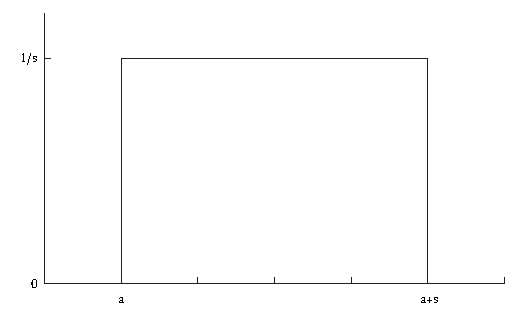
\includegraphics[width=\textwidth]{pdfUniform}
\end{center}
\caption[Uniform distribution]{Uniform distribution, $\opr{Uniform}(x\given a,s)$ \eqref{Uniform}}
\end{figure}


The standard uniform distribution is related to every other continuous distribution via the  inverse probability integral transform (Smirnov transform)\index{Smirnov transform}\index{inverse probability integral transform}. If $X$ is a random variable and $F_X^{-1}(z)$ the inverse of the corresponding cumulative distribution function then 
\[ 
X \sim F_X^{-1}\bigl( \opr{StdUniform}() \bigr) \ .  \checked
\notag
\]
If the inverse cumulative distribution function has a tractable closed form, then inverse transform sampling\index{inverse transform sampling} can provide an efficient method of sampling random numbers from the distribution of interest. See appendix~\secref{sec:random}.

The power function distribution \eqref{PowerFn} is related to the uniform distribution via a Weibull transform.
\[
\opr{PowerFn}(a,s,\beta) \sim a + s\ \opr{StdUniform}()^{\tfrac{1}{\beta}}  \checked
\notag
\]

The sum of $n$ independent standard uniform variates is the  Irwin-Hall \eqref{IrwinHall} distribution,
\[
\sum_{i=1}^{n} \opr{Uniform}_i(0,1)  \sim \opr{IrwinHall}(n) \checked
\notag
\]
and the product is the uniform-product distribution \eqref{UniformProduct}.
\[
\prod_{i=1}^{n} \opr{Uniform}_i(0,1)  \sim \opr{UniformProduct}(n) \checked
\notag
\]


% !TEX encoding = UTF-8 Unicode 
% !TEX root = FieldGuide.tex

\begin{table*}[t!]
\caption[Uniform distribution -- Properties]{Properties of the uniform distribution}
\begin{align*}
\text{\hyperref[PropertiesSec]{Properties}}  \quad& \\
\text{notation} \quad & \text{Uniform}(x \given a,s) 				\checked
\\
\text{PDF} \quad & \frac{1}{|s|}								\checked
\\
\text{CDF} \big/ \text{CCDF} \quad  &  \tfrac{x-a}{s} & s>0 \ \big/ \   s<0 
\\
\text{parameters} \quad & a,\ s \text{ in }  \mathbb{R}			\checked
\\
\text{support} \quad &  \phantom{s+{}} a \leq x \leq a+s      & s>0					\checked
\\
				&    a+s \leq x \leq a    & s<0					\checked
\\
\text{median} \quad  & a + \half s							\checked
\\
\text{mode} \quad  & \text{any supported value }				\checked
\\
\text{mean} \quad  & a + \half s								\checked
\\
\text{variance} \quad  & \sfrac{1}{12}s^2						\checked
\\
\text{skew} \quad  & 0									\checked
\\
\text{kurtosis} \quad  & -\tfrac{6}{5}							\checked
\\
\text{entropy} \quad  & \ln |s|  								\checked
\\
\text{MGF} \quad  &  \frac{e^{at}( e^{st}- 1 ) }{ |s| t}				%Double double check
\\
\text{CF} \quad  & \frac{e^{iat} (e^{i st})-1 }{ i |s| t}				%Double double check
\end{align*}

\end{table*}





% !TEX encoding = UTF-8 Unicode 
% !TEX root = FieldGuide.tex

\Sec{Exponential Distribution}
\label{sec:Exp}
\dist{Exponential} (Pearson type X, waiting time, negative exponential, inverse exponential) distribution~\cite{Pearson1916,Kondo1930,Johnson1994}:
%
\begin{align}
\label{Exp}
\opr{Exp}(x \given a, \theta) 
= & \frac{1}{|\theta|} \exp\left\{-\frac{x-a}{\theta}\right\} 	\checked
\\ \notag 
& a,\ \theta, \text{ in } \mathbb{R}  					\checked
\\ \notag
\text{support } & x > a, \quad \theta>0 				\checked
\\ \notag
& x < a, \quad \theta<0 							\checked
\end{align}
An important property of the exponential distribution is that it is memoryless\index{memoryless}: assuming positive scale and zero location ($a=0,\ \theta>0$) the conditional probability given that $x>c$, where $c$ is a positive content, is again an exponential distribution with the same scale parameter. The only other distribution with this property is the geometric distribution\index{geometric distribution}, the discrete analog of the exponential distribution. The exponential is the maximum entropy distribution given the mean and semi-infinite support. 



% !TEX encoding = UTF-8 Unicode 
% !TEX root = FieldGuide.tex

\begin{table*}[t!]
\caption[Exponential distribution -- Properties]{Properties of the exponential distribution}
\begin{align*}
\text{\hyperref[PropertiesSec]{Properties}}  \quad& \\
\text{notation} \quad & \op{Exp}(x\given a,\theta)					\checked
\\
\text{PDF}\quad &    \frac{1}{|\theta|} \exp\Left\{-\frac{x-a}{\theta}\Right\} 	\checked
\\
\text{CDF}\big  / \text{CCDF}  \quad  &   1- \exp\Left\{-\frac{x-a}{\theta}\Right\} & \theta>0 \ \big{/} \  \theta<0
\checked
\\
\text{parameters}\quad &   a,\ \theta, \text{ in } \Real 				\checked
\\
\text{support} \quad &   [ a, +\infty]      & \theta>0					\checked
\\
				&   [-\infty,  a]     & \theta <0					\checked
\\
\text{median} \quad  &  a + \theta \ln 2							\checked
\\
\text{mode} \quad  & a										\checked
\\
\text{mean} \quad  &  a+ \theta									\checked						
\\
\text{variance} \quad  & \theta^2								\checked
\\
\text{skew} \quad  &  2										\checked
\\
\text{ex. kurtosis} \quad  &  6										\checked
\\
\text{entropy} \quad  & 1 + \ln |\theta|							\checked
\\
\text{MGF} \quad  & \frac{\exp(at) }{ \Left(1- \theta t\Right)}				\checked
\\
\text{CF} \quad  & \frac{\exp(iat) }{ \Left(1- i \theta t\Right)}				\checked
\end{align*}
\end{table*}



\SSec{Special cases}
\phantomsection\addcontentsline{toc}{subsection}{~~~~~~~~~~~~Anchored exponential}
\phantomsection\addcontentsline{toc}{subsection}{~~~~~~~~~~~~Standard exponential}
The exponential distribution is commonly defined with zero location and positive scale ({\bf anchored exponential}).
With $a=0$ and $\theta=1$ we obtain the {\bf standard exponential} distribution. 

\begin{figure}[tb]
\begin{center}
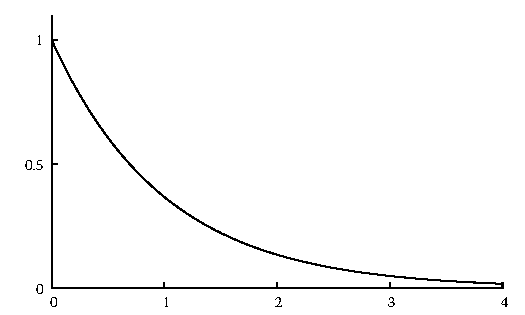
\includegraphics[width=\textwidth]{pdfStdExp}
\end{center}
\caption[Standard exponential distribution]{Standard exponential distribution, $\opr{Exp}(x\given 0,1)$}
\end{figure}


\SSec{Interrelations}

The exponential distribution is common limit of many distributions.
\begin{align*}
	\opr{Exp} (x\given a,\theta)  
	 &	=  \opr{Amoroso}(x\given  a ,\theta,1,1) 	\checked
\\&		\qquad= \opr{Gamma}(x \given a , \theta, 1)	\checked
\\	\opr{Exp} (x\given 0,\theta)  &	=  \opr{Amoroso}(x\given  0 ,\theta,1,1) \checked
 \\ & \qquad =  \opr{Gamma}(x\given  0, \theta,1)  \checked
\\
\opr{Exp}(x\given a,\theta) &=  \lim_{\beta\rightarrow\infty} \opr{PowerFn} (x\given a-\beta\theta,\beta\theta,\beta) 
\checked
\end{align*}

The sum of independent exponentials is an Erlang distribution, a special case of the gamma distribution~\eqref{Gamma}.
\[
\sum_{i=1}^{n} \opr{Exp}_i(0,\theta) \sim \opr{Gamma}(0, \theta, n) \checked
\]


The minima of a collection of exponentials, with positive scales $\theta_i>0$, is  also exponential,
\[
\op{min}\bigl( \opr{Exp}_1(0,\theta_1),\ \opr{Exp}_2(0,\theta_2),\ \ldots\ ,\ \opr{Exp}_n(0,\theta_n) \bigr) \sim \opr{Exp}(0, \theta') \, , \checked
\]
where $\theta' = (\sum_{i=1}^{n} \tfrac{1}{\theta_i})^{-1}$. \checked


The order statistics \secref{OrderStatistic} of the exponential distribution are the beta-exponential distribution~\eqref{BetaExp}.
\begin{align*}
\opr{OrderStatistic}&_{\opr{Exp}(\pLoc,\pScale)}  (x \given \alpha, \gamma) =  \opr{BetaExp}(x\given \pLoc, \pScale, \alpha, \gamma)  \checked
\end{align*}


A Weibull transform of the standard exponential distribution yields the Weibull distribution  \eqref{Weibull}.
\[
\opr{Weibull}(a,\theta,\beta) \sim a+ \theta\ \oprr{StdExp}{Exp}()^{\tfrac{1}{\beta}} \checked
\]


The ratio of independent anchored exponential distributions is the exponential ratio distribution \eqref{ExpRatio}, a special case of the beta prime distribution \eqref{BetaPrime}.
\label{sec:ExpRatio}
\[
\opr{BetaPrime}(0,\tfrac{\theta_1}{\theta_2} , 1,1) \sim \opr{ExpRatio}(0,\tfrac{\theta_1}{\theta_2}) \sim \frac{\opr{Exp}_1(0,\theta_1)}{\opr{Exp}_2(0,\theta_2) }
\]



% !TEX encoding = UTF-8 Unicode 
% !TEX root = FieldGuide.tex

\Sec{Laplace Distribution} 
\label{sec:Laplace}
\dist{Laplace} (Laplacian, double exponential, Laplace's first law of error, two-tailed exponential, bilateral exponential, biexponential) distribution~\cite{Laplace1774,Stigler1986,Kotz2001}
 is  a two parameter, symmetric, continuous, univariate, unimodal probability density with infinite support, smooth expect for a single cusp.
The functional form is
\begin{align}
\label{Laplace}
\opr{Laplace}(x\given \pLoc, \theta) = & 
\frac{1}{2 |\theta|} e^{- \left| \frac{x-\pLoc}{\theta}\right|} 		\checked
\\
\notag
& \text{for } x,\ \pLoc,\  \theta \text{ in }  \mathbb{R}			\checked
\end{align}
The two real parameters consist of a location parameter $\pLoc$,  and a scale parameter $\theta$.




\SSec{Special cases}
\phantomsection\addcontentsline{toc}{subsection}{~~~~~~~~~~~~Standard Laplace}
The {\bf standard Laplace} (Poisson's first law of error) distribution occurs when $\pLoc=0$ and $\theta=1$.



\SSec{Interrelations}

The Laplace distribution is a limit of the symmetric beta-logistic~\eqref{SymBetaLogistic}, exponential power~\eqref{ExpPower} and generalized Pearson VII~\eqref{GenPearsonVII} distributions.

As $\theta$ limits to infinity, the Laplace distribution limits to a degenerate distribution. In the alternative limit that $\theta$ limits to zero, we obtain an indefinite uniform distribution.


The difference between two independent identically distributed exponential random variables is Laplace, and therefore so is the time difference between two independent Poisson events.
\[
\opr{Laplace}(\pLoc, \theta) \sim  \opr{Exp}(\pLoc,\theta) - \opr{Exp}(\pLoc,\theta)
\]

Conversely, the absolute value (about the centre of symmetry) is exponential. 
\[
\opr{Exp}(\pLoc, |\theta|) \sim  |\opr{Laplace}(\pLoc,\theta) - \pLoc | +\pLoc
\]


The log ratio of standard uniform distributions is a standard Laplace.
\[
\opr{Laplace}(0,1) \sim \ln \frac{\opr{StdUniform}_1() }{\opr{StdUniform}_2()} \checked
\]


The Fourier transform of a standard Laplace distribution is the standard Cauchy distribution \eqref{Cauchy}.
\[
\int_{-\infty}^{+\infty} \frac{1}{2}e^{-| x |} e^{i t x} dx = \frac{1}{1+t^2}
\checked
\]



\begin{figure}[t!]
\begin{center}
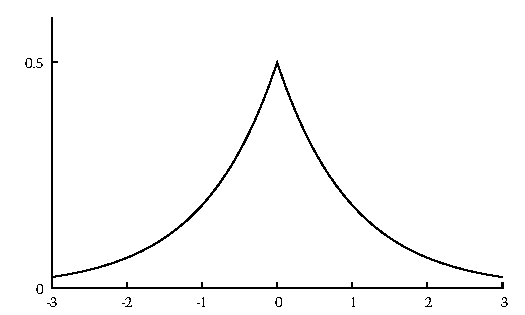
\includegraphics[width=\textwidth]{pdfLaplace}
\end{center}
\caption[Standard Laplace distribution]{Standard Laplace distribution, $\opr{Laplace}(x\given 0,1)$}
\end{figure}


% !TEX encoding = UTF-8 Unicode 
% !TEX root = FieldGuide.tex

\begin{table*}[t!]
\caption[Laplace distribution -- Properties]{Properties of the Laplace distribution}
\begin{align*}
\text{\hyperref[PropertiesSec]{Properties}}  \quad& \\
\text{notation}\quad & \op{Laplace}(x\given \pLoc, \theta) 				\checked
\\ 
\text{PDF} \quad & \frac{1}{2 |\theta|} e^{- \Left|\frac{x-\pLoc}{\theta}\Right|} 	\checked
\\
\text{CDF} \quad & 
\begin{cases}
\phantom{\tfrac{1}{2} -\ } \frac{1}{2} e^{ - \Left|\frac{x-\pLoc}{\theta}\Right| } & x\leq \pLoc  \checked
\\
1 - \tfrac{1}{2} e^{ - \Left|\frac{x-\pLoc}{\theta}\Right| } & x\geq \pLoc 			\checked
\end{cases}
\\
\text{parameters}\quad & \pLoc,\ \theta \text{ in } \mathbb{R}				\checked
\\
\text{support} \quad & x \in [ -\infty, +\infty] 							\checked
\\
\text{median} \quad & \pLoc                            							\checked
\\
\text{mode} \quad & \pLoc 										\checked
\\
\text{mean} \quad & \pLoc  										\checked
\\
\text{variance} \quad & 2\theta^2 									\checked
\\
\text{skew} \quad & 0 											\checked
\\ 
\text{kurtosis} \quad & 3 											\checked
\\ 
\text{entropy} \quad & 1+ \ln( 2 \theta) 								\checked
\\ 
\text{MGF} \quad &  \frac{\exp(\pLoc t) }{1- \theta^2 t^2}					\checked
\\
\text{CF} \quad & \frac{\exp(i\pLoc t) }{1+ \theta^2 t^2}					\checked
\end{align*}
\end{table*}


% !TEX encoding = UTF-8 Unicode 
% !TEX root = FieldGuide.tex

\Sec{Normal Distribution}
\label{sec:Normal}
\phantomsection\addcontentsline{toc}{subsection}{~~~~~~~~~~~~Normal} 
The  {\bf Normal} (Gauss, Gaussian, bell curve, Laplace-Gauss, de Moivre, error, Laplace's second law of error, law of error)~\cite{Moivre1733,Johnson1994} distribution is a ubiquitous two parameter, continuous, univariate unimodal probability distribution with infinite support, and an iconic bell shaped curve. 
%
\begin{align}
\label{Normal}
\opr{Normal}(x\given \mu,\sigma) 
&=
\frac{1}{\sqrt{2 \pi \sigma^2}}  \exp\left\{ - \frac{( x-\mu)^2}{2\sigma^2} \right\} \checked
\\
& \text{for } x,\ \mu,\  \sigma \text{ in }  \mathbb{R}						\checked 
\notag
\end{align}
The location parameter $\mu$ is the mean, and the scale parameter $\sigma$ is the standard deviation. Note that the normal distribution is often parameterized with the variance $\sigma^2$ rather than the standard deviation. Herein, we choose to consistently parameterize distributions with a scale parameter.  

The normal distribution most often arises as a consequence of the famous central limit theorem, which states (in its simplest form) that the mean of independent and identically distribution random variables, with finite mean and variance, limit to the normal distribution as the sample size becomes large. 
\index{central limit theorem}
The normal distribution is also the maximum entropy distribution for fixed mean and variance.




\SSec{Special cases}
\phantomsection\addcontentsline{toc}{subsection}{~~~~~~~~~~~~Error function}
\phantomsection\addcontentsline{toc}{subsection}{~~~~~~~~~~~~Standard normal}
With $\mu=0$ and $\sigma = 1/ \sqrt{2} h$ we obtain the {\bf error function} distribution, and
with $\mu=0$ and $\sigma=1$ we obtain the {\bf standard normal} ($\Phi$, $z$, unit normal)  distribution. 


 \SSec{Interrelations}
 In the limit that $\sigma\rightarrow\infty$ we obtain an unbounded uniform (flat) distribution, and in the limit $\sigma\rightarrow0$ we obtain a degenerate (delta) distribution. 
 
The normal distribution is a limiting form of many distributions, including the gamma-exponential \eqref{GammaExp}, Amoroso \eqref{Amoroso} and Pearson IV \eqref{PearsonIV} families and their superfamilies. 



Many distributions are transforms of normal distributions.
\begin{align*}
\exp\bigl(\opr{Normal}(\mu,\sigma) \bigr) &\sim \opr{LogNormal}(0, e^\mu, \sigma) & \eqref{LogNormal}  \checked
\\
\big| \opr{Normal}(0,\sigma) \big|  & \sim  \opr{HalfNormal}( \sigma) & \eqref{HalfNormal} \checked
\\
\oprr{StdNormal}{Normal}()^{2} & \sim \opr{ChiSqr}(1)  & \eqref{ChiSqr}  \checked
\\
\sum_{i=1,k}\oprr{StdNormal}{Normal}_i()^{2} & \sim \opr{ChiSqr}(k)  & \eqref{ChiSqr} \checked
\\
\opr{Normal}(0,\sigma)^{-2} & \sim \Levy( 0, \tfrac{1}{\sigma^2})   & \eqref{Levy}  \checked
\\
\big|\opr{Normal}(0,\sigma)\big|^{\tfrac{2}{\beta}} & \sim \opr{Stacy}( (2\sigma^2)^{\tfrac{1}{\beta}}, \tfrac{1}{2}, \beta )  & \eqref{Stacy}  
\\
\frac{\oprr{StdNormal}{Normal}_1()}{\oprr{StdNormal}{Normal}_2()}  & \sim  \opr{StdCauchy}() &\eqref{StdCauchy} \checked
\end{align*}



\begin{figure}[t]
\begin{center}
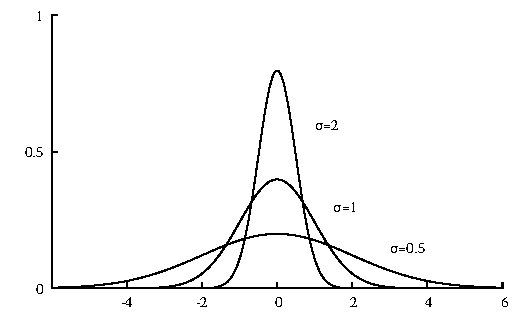
\includegraphics[width=\textwidth]{pdfNormal}
\end{center}
\caption[Normal distributions]{Normal distributions, $\opr{Normal}(x\given 0,\sigma)$}
\end{figure}


The normal distribution is stable \eqref{Stable}. That is a sum of independent normal random variables is also normally distributed.
\[
 \opr{Normal}_1(\mu_1,\sigma_1) +  \opr{Normal}_2(\mu_2,\sigma_2) \sim  \opr{Normal}_3(\mu_1+\mu_2,\sigma_1+\sigma_2)
\checked
\notag
\]
\index{stable distributions}

The Box-Muller transform~\cite{Box1958} generates pairs of independent normal variates from pairs of uniform random variates.
\begin{align*}
\oprr{StdNormal}{Normal}_1() & \sim \opr{ChiSqr}(1)\ \cos\bigl( 2\pi\ \opr{StdUniform}_2() \bigr) \checked
\\
\oprr{StdNormal}{Normal}_2() & \sim \opr{ChiSqr}(1)\ \sin\bigl( 2\pi\ \opr{StdUniform}_2() \bigr) \checked
\\
\text{where }& \opr{ChiSqr}(1) \sim\sqrt{ - 2 \ln \opr{StdUniform}_1()}  \checked
\end{align*}
Nowadays more efficient random normal generation methods are generally employed~\secref{sec:random}.




% !TEX encoding = UTF-8 Unicode 
% !TEX root = FieldGuide.tex

\begin{table*}[t!]
\caption[Normal distribution -- Properties]{Properties of the normal distribution}

\begin{align*}
\text{\hyperref[PropertiesSec]{Properties}}  \quad& \\
\text{notation} \quad & \op{Normal}(x\given \mu,\sigma)	\checked
\\
\text{PDF}\quad &   \frac{1}{\sqrt{2 \pi \sigma^2}}  \exp\left\{ - \frac{( x-\mu)^2}{2\sigma^2} \right\} \checked
\\
\text{CDF} \quad  &   \frac{1}{2}\left[  1 + \text{erf}\left(\frac{x-\mu}{\sqrt{2 \sigma^2}} \right) \right]	\checked
\\
\text{parameters}\quad &   \mu,\ \sigma \text{ in } \mathbb{R}						\checked
\\
\text{support} \quad &   x \in [-\infty, + \infty]									\checked
\\
\text{median} \quad  &  \mu												\checked
\\
\text{mode} \quad  & \mu													\checked
\\
\text{mean} \quad  &  \mu													\checked
\\
\text{variance} \quad  & \sigma^2											\checked
\\
\text{skew} \quad  &  0													\checked
\\
\text{kurtosis} \quad  &  0													\checked
\\	
\text{entropy} \quad  & \tfrac{1}{2} \ln(2\pi e \sigma^2)							\checked
\\
\text{MGF} \quad  &  \exp\left({\mu t + \tfrac{1}{2} \sigma^2 t^2 }\right)				\checked
\\
\text{CF} \quad  &  \exp\left({i \mu t - \tfrac{1}{2} \sigma^2 t^2}\right)					\checked
\end{align*}

\end{table*}






% One shape parameter

% !TEX encoding = UTF-8 Unicode 
% !TEX root = FieldGuide.tex

\subpart{One shape parameter}


\Sec{Power Function Distribution}
\label{sec:PowerFn}


\dist{Power function} (power) distribution~\cite{Pearson1916, Meniconi1996,Johnson1995} 
is  a three parameter, continuous, univariate, unimodal probability density, with finite or semi-infinite support. The functional form in most straightforward  parameterization consists of a single power function.
\begin{align}
\label{PowerFn}
\opr{PowerFn}(x\given a,s,\beta) &= 
\left|\frac{\beta}{ s}\right|
\left(\frac{x-a}{s} \right)^{\beta -1} \checked
%\\ &= \opr{GenBeta}(x\given a,s , \alpha,1,1) \notag 
\\
\notag  \text{for } & x, a, s, \beta \text{ in } \mathbb{R}
 \\ \text{ support } & x \in [a,a+s], s>0,\ \beta>0 \notag \checked
  \\ \text{ or } &  x\in[a+s,a], s<0,\ \beta>0  \checked
 \notag 
 \\  \notag  \text{ or } &  x\in[a+s,+\infty], s>0,\ \beta<0 \checked
 \\  \notag  \text{ or } &  x\in[-\infty,a+s], s<0,\ \beta<0 \checked
 \notag
\end{align}
%
%Pearson~\cite{Pearson1916, Johnson1994} noted two special cases, the monotonically decreasing {\bf Pearson type VIII} $0<\beta <1$, and the monotonically increasing {\bf Pearson type IX} distribution~\cite{Pearson1916, Johnson1994} with $\beta>1$. 
With positive $\beta$ we obtain a distribution with finite support. But by allowing $\beta$ to extend to negative numbers, the power function distribution also encompasses the semi-infinite Pareto distribution \eqref{Pareto}, and in the limit $\beta\rightarrow\infty$ the exponential distribution \eqref{Exp}.


\SSec{Alternative parameterizations}

% CITATION NEEDED
\dist{Generalized Pareto} distribution: An alternative parameterization that emphasizes the limit to exponential.
\begin{align}
\label{GenPareto}
\opr{GenPareto}&(x\given a',s',\xi) 
\\ & =
 \begin{cases}
  \frac{1}{|\theta|}\left( 1 + \xi \frac{x-\pLoc}{\theta}\right)^{-\tfrac{1}{\xi}-1} & \xi \neq 0 \checked
\notag
\\ 
 \frac{1}{|\theta|} \exp \left(-\frac{x-\pLoc}{\theta} \right)& \xi = 0 \checked
\notag
\end{cases}
\\
& = \opr{PowerFn}(x\given \pLoc-\tfrac{\theta}{\xi},\tfrac{\theta}{\xi},  -\tfrac{1}{\xi}) \checked
\notag
\end{align}


% CITATION NEEDED
\dist{q-exponential} (generalized Pareto) distribution is an alternative parameterization of the power function distribution, utilizing the Tsallis generalized q-exponential function, $\exp_q(x)$ \secref{sec:Limits}.
\begin{align}
\label{QExp}
\opr{QExp}&(x\given  \pLoc,\theta,q) \\
\notag
= & \frac{(2-q)}{|\theta|} \exp_q\left(- \frac{x-\pLoc}{\theta} \right)  \checked
\\  
= &
\begin{cases}
\frac{(2-q)}{|\theta|}\left(1 - (1-q) \frac{x-\pLoc}{\theta} \right)^{\frac{1}{1-q}} & q \neq 1 \checked
\\
\notag
\tfrac{1}{|\theta| }\exp\left(- \frac{x-\pLoc}{\theta} \right)  & q=1 \checked
\end{cases}
\notag
\\
=&  \opr{PowerFn}(x\given \pLoc+\frac{\theta}{1-q},-\frac{\theta}{1-q},\frac{2-q}{1-q}) \checked
\\
\notag  \text{for } & x, \pLoc, \theta, q \text{ in } \mathbb{R}
\end{align}



\begin{figure}[p]
\begin{center}
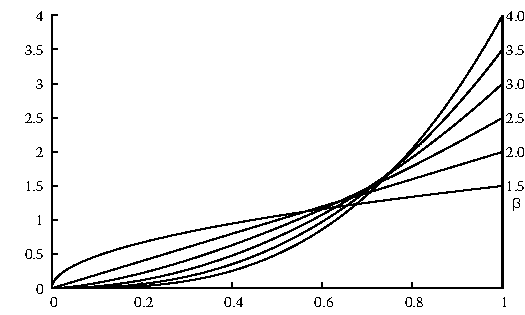
\includegraphics[width=\textwidth]{pdfPowerFn}
\end{center}
\caption[Pearson IX distributions]{Pearson type IX, $\opr{PowerFn}(x\given 0,1,\beta)$, $\beta>1$
}
\end{figure}
%
%
\begin{figure}[p]
\begin{center}
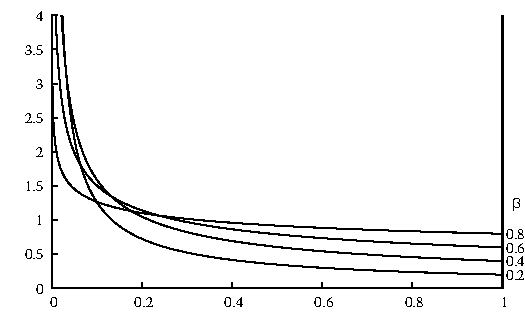
\includegraphics[width=\textwidth]{pdfPowerFn2}
\end{center}
\caption[Pearson VIII distributions]{Pearson type VIII, $\opr{PowerFn}(x\given 0,1,\beta)$, $0<\beta<1$. }
\end{figure}
%
\begin{figure}[tp]
\begin{center}
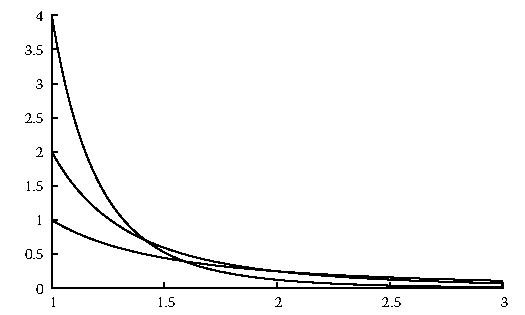
\includegraphics[width=\textwidth]{pdfPareto}
\end{center}
\caption[Pareto distributions]{Pareto distributions, $\opr{Pareto}(x\given 0,1,\bar\beta)$, $\bar\beta$ left axis.}
\end{figure}




\SSec{Special cases: Positive \texorpdfstring{$\beta$}{beta}}
\phantomsection\addcontentsline{toc}{subsection}{~~~~~~~~~~~~Pearson IX} 
\phantomsection\addcontentsline{toc}{subsection}{~~~~~~~~~~~~Pearson VIII} 
Pearson~\cite{Pearson1916, Johnson1994} noted two special cases, the monotonically decreasing {\bf Pearson type VIII} $0<\beta <1$, and the monotonically increasing {\bf Pearson type IX} distribution~\cite{Pearson1916, Johnson1994} with $\beta>1$. 


\dist{Wedge} distribution~\cite{Johnson1994}: 
\begin{align}
\label{Wedge}
\opr{Wedge}(x\given a,s) &= 2\ \op{sgn}(s) \frac{x-a}{s^2} \checked
\\& = \opr{PowerFn}(x\given a,s,2) \notag \checked
\end{align}
With a positive scale we obtain an {\bf ascending wedge} (right triangular) distribution, and with negative scale a {\bf descending wedge} (left triangular). 
\phantomsection\addcontentsline{toc}{subsection}{~~~~~~~~~~~~Ascending wedge}
\phantomsection\addcontentsline{toc}{subsection}{~~~~~~~~~~~~Descending wedge}

\SSec{Special cases: Negative \texorpdfstring{$\beta$}{beta}}

\dist{Pareto} (Pearson XI, Pareto type I) distribution~\cite{Pareto1964, Pearson1916, Johnson1994}:
\begin{align}
\label{Pareto}
\opr{Pareto}(x\given a,s,\gamma) &= \left| \frac{\bar{\beta}}{s}\right| \left(\frac{x-a}{s}\right)^{-\bar{\beta}-1}   \qquad \bar{\beta}>0
\checked
\\ \notag & \qquad x > a+s, \ s>0
\\ \notag & \qquad x < a+s, \ s<0
 \\ \notag &= \opr{PowerFn}(x\given a, s, -\bar{\beta}) \checked
\end{align}
The most important special case is the Pareto distribution, which has a semi-infinite support with a power-law tail. The Zipf distribution \index{Zipf distribution} is the discrete analog of the Pareto distribution.


\dist{Lomax} (Pareto type II, ballasted Pareto) distribution~\cite{Lomax1954}: 
\begin{align}
\label{Lomax}
\opr{Lomax}(x\given a, s, \gamma) &= \frac{\gamma}{|s|}  \left(1+\frac{x-a}{s}\right)^{-\gamma-1} 
\\ \notag & = \opr{Pareto}(x\given a-s, s, \gamma)  
\\ \notag & = \opr{PowerFn}(x \given a-x, s, -\gamma) 
\end{align}
Originally explored as a model of business failure. The alternative name ``ballasted Pareto'' arises since this distribution is a shifted Pareto distribution~\eqref{Pareto} whose origin is fixed at zero, and no longer moves with changes in scale.



\dist{Exponential ratio} distribution~\cite{\self}:
\begin{align}
\label{ExpRatio}
\opr{ExpRatio}(x\given s) &= \frac{1}{|s|} \frac{1}{\left(1+\frac{x}{s}\right)^{2}} 	\checked
& \\ \notag &= \opr{Lomax}(x\given 0, s,1)
& \\ \notag &= \opr{PowerFn}(x\given -s, s,1)
\end{align}
Arises as the ratio of independent exponential distributions (p~\pageref{sec:ExpRatio}).


\dist{Uniform-prime} distribution~\cite{Jones2004,\self}:
\begin{align}
\label{UniPrime}
\opr{UniPrime}(x\given a,s) &= \frac{1}{|s|} \frac{1}{\left(1+\frac{x-a}{s}\right)^{2}}  
& \\ \notag &= \opr{Lomax}(x\given a, s,1)
& \\ \notag &= \opr{PowerFn}(x\given a-s, s,-1) 
\end{align}
An exponential ratio~\eqref{ExpRatio} distribution with a shift parameter. So named since this distribution is related to the uniform distribution as beta is to beta prime. The ordering distribution \secref{OrderStatistic} of the beta-prime distribution.
%
% Mentioned in Jones2004, sec 6.2, as $F_{2,2}$ and in section 6.3.2 as ordering distribution






\begin{table*}[tp]
\caption[Power function distribution -- Special cases]{Special cases of the power function distribution}
\begin{center}
{\renewcommand{\arraystretch}{1.25} 
\begin{tabular}{llccc@{\extracolsep{5pt}} l}
\eqref{PowerFn} &power function& $a$ & $s$ & $\beta$ &
\\ \hline
%\eqref{PowerLaw} & Jeffreys	& . & s & -$0$ & $\lim_{s\rightarrow\infty}$\\
%\eqref{PowerLaw} & Power-law		& . & s & $<\!\!0$ & $\lim_{s \rightarrow\infty}$\\
\eqref{Pareto} & Pareto		& . & . & $<\!\!0$ & \\
\eqref{PowerFn} & Pearson type VIII 		& 0 & . &  $(0,1)$ &\\
\eqref{Uniform} & uniform		& . & . & $1$ &\\
\eqref{PowerFn} & Pearson type IX 		& 0 & .  & $>\!\!1$ & \\
\eqref{Wedge} & wedge			& . & . & 2 & \\
\eqref{Exp} & exponential			& . & . & +$\infty$ & \\
\end{tabular} 
}
\end{center}
\end{table*}

%
% !TEX encoding = UTF-8 Unicode 
% !TEX root = FieldGuide.tex

\begin{table*}[t!]
\caption[Power function distribution -- Properties]{Properties of the power function distribution}
\begin{align*}
\text{\hyperref[PropertiesSec]{Properties}}  \quad& \\
\text{notation}\quad &   \text{PowerFn}(x\given a,s,\beta) 
\\
\text{PDF}\quad &   \Left|\frac{\beta}{ s}\Right|\Left(\frac{x-a}{s} \Right)^{\beta -1}  \checked
\\
 \text{CDF}  \big/ \text{CCDF} \quad  &   \Left(\frac{x-a}{s} \Right)^{\beta } & \tfrac{s}{\beta}  >0 \ \big{/} \ \tfrac{s}{\beta}<0  \checked
\\
\text{parameters}\quad &   a, s, \beta \text{ in } \Real
\\
\text{support} \quad &    x \in [a,a+s] & s>0,\ \beta >0 \checked
 \\ 			 &  x\in[a+s,a] &s<0,\ \beta >0   \checked
 \\  			 &  x\in[a+s,+\infty]& s>0,\ \beta<0 \checked
 \\  			&  x\in[-\infty,a+s] & s<0,\ \beta<0  \checked
\\
%\text{median} \quad  &  \cdots
%\\
\text{mode} \quad  & a & \beta >0 \checked
\\
& a+s & \beta <0  \checked
\\
\text{mean} \quad  &a+  \frac{s\beta}{\beta+1} &  \beta \notin [-1,0] \checked
\\
\text{variance} \quad  & \frac{ s^2 \beta }{ (\beta+1)^2 (\beta+2) } & \beta \notin [-2,0] \checked
\\
\text{skew} \quad  & \op{sgn}(\tfrac{\beta}{s})\ \frac{2(1-\beta)}{(\beta+3)}  \sqrt{\frac{\beta+2}{\beta}}
& \beta \notin [-3,0] 
\checked
\\
\text{ex. kurtosis} \quad  &  \frac{6(\beta^3-\beta ^2- 6 \beta +2)}{\beta(\beta +3)(\beta +4)} & \beta \notin [-4,0] \checked
\\
%\text{entropy} \quad  &  \ldots
%\\
\text{MGF} \quad  &  \text{undefined}
%\\
%\text{CF} \quad  & \ldots
\end{align*}
\end{table*}



 \SSec{Limits and subfamilies}

With $\beta=1$ we recover the uniform distribution.
\[
\opr{PowerFn}(a,s,1) \sim \opr{Uniform}(a,s) \checked
\]

As $\beta$ limits to infinity, the power function distribution limits to the exponential distribution \eqref{Exp}.
\begin{align*}
\opr{Exp}(x\given \nu,\lambda) &=  \lim_{\beta\rightarrow\infty} \opr{PowerFn} (x\given \nu-\beta\lambda,\beta\lambda,\beta) \checked \\
	&=  \lim_{\beta\rightarrow\infty}  \left|\frac{1}{ \lambda}\right| \left(1+\frac{x-\nu}{\beta\lambda} \right)^{\beta -1} 
	\checked
\end{align*}
Recall that $\lim_{c\rightarrow\infty} \left(1 + \frac{x}{c} \right)^{c} = e^x$. \checked



 \SSec{Interrelations}
 

With positive $\beta$, the power function distribution is a special case of the beta distribution \eqref{Beta}, with negative beta, a special case of the beta prime distribution \eqref{BetaPrime}, and with either sign a special case of the generalized beta  \eqref{GenBeta} and unit gamma \eqref{UnitGamma} distributions.
\begin{align*}
	\opr{PowerFn}& (x\given a,s,\beta) 
\\ & = \opr{GenBeta}(x\given a,s , 1,1,\beta) \checked
\\ & = \opr{GenBeta}(x\given a,s , \beta,1,1) & \beta>0 \checked
\\ & \quad = \opr{Beta}(x\given a,s , \beta,1)  & 	\beta>0	\checked
\\ & = \opr{GenBeta}(x\given a+s,s ,1,-\beta,-1) & \beta<0\checked
\\ & \quad = \opr{BetaPrime}(x\given a+s,s , 1,-\beta)  & 	\beta<0\checked
\\ & = \opr{UnitGamma}(x\given a,s,1, \beta) \checked
\end{align*}


 

The order statistics \secref{OrderStatistic} of the power function distribution yields the generalized beta distribution \eqref{GenBeta}.
\begin{align*}
\opr{OrderStatistic}_{\opr{PowerFn}(a,s,\beta)} &(x \given \alpha, \gamma)  = \opr{GenBeta}(x\given a, s, \alpha,\gamma, \beta) 
\checked
\end{align*}

Since the power function distribution is a special case of the generalized beta distribution \eqref{GenBeta},
\[
 \opr{GenBeta}(x\given a, s, \alpha,1, \beta) = \opr{PowerFn}(x\given a,s,\alpha\beta) \checked
\]
it follows that the power function family is closed under maximization for $\tfrac{\beta}{s} > 0$ and minimization for  $\tfrac{\beta}{s}<0$.



The product of independent power function distributions (With zero location parameter, and the same $\beta$) is a unit-gamma distribution \eqref{UnitGamma}~\cite{Consul1971}.
\[
\prod_{i=1}^{\alpha} \opr{PowerFn}_i(0,s_i,\beta) \sim \opr{UnitGamma}(0, \prod_{i=1}^{\alpha} s_i, \alpha, \beta) \checked
\]
Consequently, the geometric mean of independent, anchored power function distributions (with common $\beta$) is also unit-gamma.
\[
\sqrt[\alpha]{\prod_{i=1}^{\alpha} \opr{PowerFn}_i(0,s_i,\beta)} \sim \opr{UnitGamma}(0, \prod_{i=1}^{\alpha} s_i, \alpha, \alpha \beta) \checked
\]


The power function distribution can be obtained from the Weibull transform  $x\rightarrow (\tfrac{x-a}{s})^{\beta}$ of the uniform distribution \eqref{Uniform}. 
\[
\opr{PowerFn}(a,s,\beta) \sim a + s\ \opr{StdUniform}()^{\tfrac{1}{\beta}} \checked
\]

The power function distribution limits to the exponential distribution \secref{sec:Exp}.
\[
\opr{Exp}(x\given a,\theta) &=  \lim_{\beta\rightarrow\infty} \opr{PowerFn} (x\given a+\beta\theta,-\beta\theta,\beta)  
\notag
\]




% !TEX encoding = UTF-8 Unicode 
% !TEX root = FieldGuide.tex

\begin{table*}[t!]
\caption[Power function distribution -- Properties]{Properties of the power function distribution}
\begin{align*}
\text{\hyperref[PropertiesSec]{Properties}}  \quad& \\
\text{notation}\quad &   \text{PowerFn}(x\given a,s,\beta) 
\\
\text{PDF}\quad &   \Left|\frac{\beta}{ s}\Right|\Left(\frac{x-a}{s} \Right)^{\beta -1}  \checked
\\
 \text{CDF}  \big/ \text{CCDF} \quad  &   \Left(\frac{x-a}{s} \Right)^{\beta } & \tfrac{s}{\beta}  >0 \ \big{/} \ \tfrac{s}{\beta}<0  \checked
\\
\text{parameters}\quad &   a, s, \beta \text{ in } \Real
\\
\text{support} \quad &    x \in [a,a+s] & s>0,\ \beta >0 \checked
 \\ 			 &  x\in[a+s,a] &s<0,\ \beta >0   \checked
 \\  			 &  x\in[a+s,+\infty]& s>0,\ \beta<0 \checked
 \\  			&  x\in[-\infty,a+s] & s<0,\ \beta<0  \checked
\\
%\text{median} \quad  &  \cdots
%\\
\text{mode} \quad  & a & \beta >0 \checked
\\
& a+s & \beta <0  \checked
\\
\text{mean} \quad  &a+  \frac{s\beta}{\beta+1} &  \beta \notin [-1,0] \checked
\\
\text{variance} \quad  & \frac{ s^2 \beta }{ (\beta+1)^2 (\beta+2) } & \beta \notin [-2,0] \checked
\\
\text{skew} \quad  & \op{sgn}(\tfrac{\beta}{s})\ \frac{2(1-\beta)}{(\beta+3)}  \sqrt{\frac{\beta+2}{\beta}}
& \beta \notin [-3,0] 
\checked
\\
\text{ex. kurtosis} \quad  &  \frac{6(\beta^3-\beta ^2- 6 \beta +2)}{\beta(\beta +3)(\beta +4)} & \beta \notin [-4,0] \checked
\\
%\text{entropy} \quad  &  \ldots
%\\
\text{MGF} \quad  &  \text{undefined}
%\\
%\text{CF} \quad  & \ldots
\end{align*}
\end{table*}



% !TEX encoding = UTF-8 Unicode 
% !TEX root = FieldGuide.tex

\Sec{Log-Normal Distribution} 
\label{sec:LogNormal}
\dist{Log-normal} (Galton, Galton-McAlister, anti-log-normal, Cobb-Douglas, log-Gaussian, logarithmic-normal, logarithmico-normal, $\Lambda$, Gibrat) distribution \cite{Galton1879, McAlister1879, Johnson1994}
 is  a three parameter, continuous, univariate, unimodal probability density with semi-infinite support. The functional form in the standard  parameterization is
 \begin{align}
 \label{LogNormal}
\opr{LogNormal}&(x\given a, \vartheta,\beta) 
 \\ \notag = & \frac{|\beta|}{\sqrt{2\pi \vartheta^2}} \Left(\frac{x-a}{\vartheta}\Right)^{-1} \exp\Left\{-\frac{1}{2} \Left(\beta \ln \frac{x-a}{\vartheta} \Right)^2 \Right\}  \checked
\\ \notag
& \text{ for } x,\ a,\ \vartheta,\ \beta \  \text{in } \Real,  	
 \\ \nonumber
 & \tfrac{x-a}{\vartheta}>0
\end{align}
The log-normal is so called because the log transform of the log-normal variate is a normal random variable. The distribution should, perhaps, be more accurately called the anti-log-normal distribution, but the nomenclature is now standard. 



\SSec{Special cases}
\phantomsection\addcontentsline{toc}{subsection}{~~~~~~~~~~~~Anchored log-normal} 
\phantomsection\addcontentsline{toc}{subsection}{~~~~~~~~~~~~Gibrat} 
The {\bf anchored log-normal} (two-parameter log-normal) distribution ($a=0$) arises from the multiplicative version of the central limit theorem: When the sum of independent random variables limits to normal, the product of those random variables limits to log-normal.
With $a=0$, $\vartheta=1$, $\sigma=1$  we obtain the  {\bf standard log-normal} (Gibrat) distribution~\cite{Gibrat1931}.


\SSec{Interrelations}
The log-normal forms a location-scale-power distribution family.
\begin{align*}
\opr{LogNormal}(a, \vartheta, \beta) &\sim a+ \vartheta  \oprr{StdLogNormal}{LogNormal}()^{\frac{1}{\beta}}
\checked
\end{align*}


The log-normal distribution is the anti-log transform of a normal random variable. 
\begin{align*}
\opr{LogNormal}(a, \vartheta, \beta) &\sim a+ \exp\Bigl(- \opr{Normal}(-\ln \vartheta,\tfrac{1}{\beta})\Bigr) 
\checked
\end{align*}
Because of this close connection to the normal distribution, the log-normal is often parameterized with the mean and standard deviation of the corresponding normal distribution, $\mu=\ln \vartheta$, $\sigma=1/\beta$ rather than standard scale and power parameters. 


The log-normal distribution is a limiting form of the Unit gamma \eqref{UnitGamma} and Amoroso \eqref{Amoroso},  distributions (And therefore also of the generalized beta and generalized beta prime distributions) and limits to the normal distribution~\secref{sec:Limits}.
\[
\opr{Normal}(x\given \mu, \sigma)  =   \lim_{\beta\rightarrow\infty} \opr{LogNormal}(x\given \mu + \beta\sigma, -\beta\sigma, \beta) \checked
\notag
\]

A product of log-normal distributions (With zero location parameter) is again a log-normal distribution. This follows from the fact that the sum of normal distributions is normal.
\[
\prod_{i=1}^{n} \opr{LogNormal}_i(0, \vartheta_i, \beta_i) \sim 
\opr{LogNormal}_i(0, \prod_{i=1}^{n} \vartheta_i, (\sum_{i=0}^{n}\beta_i^{-2})^{-\half} ) 
\checked
\notag
\]


\begin{figure}[t]
\begin{center}
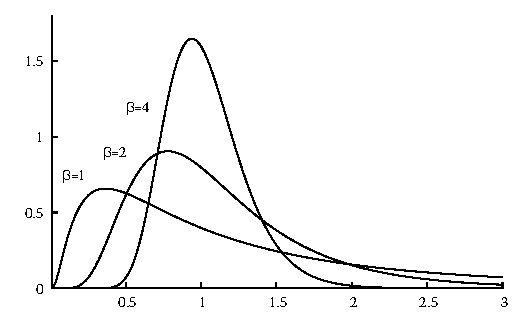
\includegraphics[width=\textwidth]{pdfLogNormal}
\end{center}
\caption[Log normal distributions]{Log normal distributions, $\opr{LogNormal}(x\given 0, 1, \beta)$}
\end{figure}







% !TEX encoding = UTF-8 Unicode 
% !TEX root = FieldGuide.tex

\begin{table*}[t!]
\caption[Log-normal distribution -- Properties]{Properties of the log-normal distribution}
 \begin{align*}
\text{\hyperref[PropertiesSec]{Properties}}  \quad& \\
\text{notation} \quad & \op{LogNormal}(x\given a, \vartheta,\beta ) \checked  	
\\
\text{PDF}\quad &   \frac{|\beta|}{\sqrt{2\pi \vartheta^2}} \left(\frac{x-a}{\vartheta}\right)^{-1} \exp\left\{-\frac{1}{2} \left( \beta \ln \frac{x-a}{\vartheta} \right)^2 \right\}	\checked					
\\
\text{CDF} \big/ \text{CCDF} \quad  &   \tfrac{1}{2} +  \tfrac{1}{2}\text{erf}\left( \sfrac{1}{\sqrt{2}} \beta \ln \frac{x-a}{\vartheta} \right) \checked
& \hspace{-2em} \vartheta >0 \ \big/ \ \vartheta <0
\\
\text{parameters}\quad &   a,\  \vartheta,\ \beta \text{ in } \Real		 \checked
\\
\text{support} \quad &   x \in [a, +\infty] \quad \vartheta>0 \checked
\\
& x \in [-\infty,a] \quad \vartheta<0 \checked
\\
\text{median} \quad  &  a+ \vartheta \checked
\\
\text{mode} \quad  & a+ \vartheta e^{-\beta^{-2}} \checked
\\
\text{mean} \quad  &  a + \vartheta e^{\tfrac{1}{2} \beta^{-2}} \checked
\\
\text{variance} \quad  & \vartheta^2 (e^{\beta^{-2}} -1) e^{\beta^{-2}} \checked
\\
\text{skew} \quad  &  ( e^{\beta^{-2}} +2) \sqrt{e^{\beta^{-2}} -1} \checked
\\
\text{kurtosis} \quad  &  e^{4\beta^{-2}} +2e^{3\beta^{-2}} +3e^{2\beta^{-2}} -6 \checked
\\
\text{entropy} \quad  & \tfrac{1}{2} + \tfrac{1}{2} \ln(2\pi\beta^{-2}) + \ln | \vartheta | \checked
\\
\text{MGF} \quad  &  \text{doesn't exist in general} \checked
\\
\text{CF} \quad  &  \text{no simple closed form expression} \checked
\end{align*}
\end{table*}




% !TEX encoding = UTF-8 Unicode 
% !TEX root = FieldGuide.tex

\Sec{Gamma Distribution}
\label{sec:Gamma}
\dist{Gamma} ($\Gamma$, Pearson type III)  distribution~\cite{Pearson1893, Pearson1895, Johnson1994} : 
%
\begin{align}
\label{Gamma}
\opr{Gamma}(x \given a, \theta, \alpha) 
&=  \frac{1}{\Gamma(\alpha)|\theta|} \Left(\frac{x-a}{\theta}\Right)^{\alpha-1} \exp\Left\{-\frac{x-a}{\theta}\Right\}  \checked
\\
\text{for } & x,\ a, \theta, \alpha \In  \mathbb{R}, \quad \alpha>0			
\notag												\checked
\\&=  \opr{Amoroso}(x\given  a, \theta, \alpha, 1) \notag 					\checked
\end{align}
The name of this distribution derives from the normalization constant.



\SSec{Special cases}
\phantomsection\addcontentsline{toc}{subsection}{~~~~~~~~~~~~Wein}
\phantomsection\addcontentsline{toc}{subsection}{~~~~~~~~~~~~Erlang}

Special cases of the beta prime distribution are listed in table~\ref{AmorosoTable}, under $\beta=1$.

The gamma distribution often appear as a solution to problems in statistical physics. For example, the energy density of a classical ideal gas, or the {\bf Wien} (Vienna) distribution $\op{Wien}(x\given T)=\opr{Gamma}(x\given 0, T,4)$, an approximation to the relative intensity of black body radiation as a function of the frequency. The {\bf Erlang} (m-Erlang) distribution~\cite{Erlang1909} is a gamma distribution with integer $\alpha$, which models the waiting time to observe $\alpha$ events from a Poisson process with rate $1/\theta$ ($\theta>0$). For $\alpha=1$ we obtain an exponential distribution \eqref{Exp}.


\begin{figure}[tp!]
\begin{center}
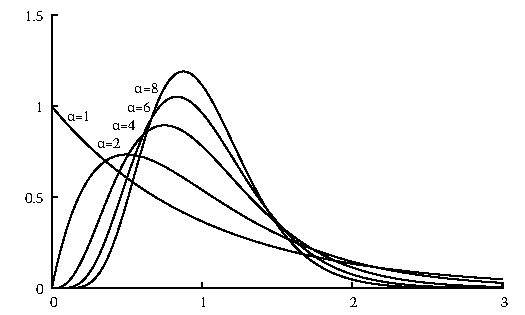
\includegraphics[width=\textwidth]{pdfGammaPDF}
\end{center}
\caption[Gamma distributions, unit variance]{Gamma distributions, unit variance $\opr{Gamma}(x\given \tfrac{1}{\alpha},\alpha)$}
\end{figure}



\dist{Standard gamma} (standard Amoroso) distribution~\cite{Johnson1994}: 
\[
\opr{StdGamma}(x\given \alpha) & = \frac{1}{\Gamma(\alpha)} x^{\alpha-1} e^{-x}		\checked
\label{StdGamma}
\\ & = \opr{Gamma}(x\given 0, 1, \alpha)\notag
\]
    

\dist{Chi-square} ($\chi^2$)  distribution~\cite{Fisher1924,Johnson1994}:
\begin{align}
\label{ChiSqr}
\opr{ChiSqr}(x \given k) 
&= \frac{1}{2\Gamma(\tfrac{k}{2})} \Left(\frac{x}{2}\Right)^{\tfrac{k}{2}-1} 
\exp\Left\{-\Left(\frac{x}{2}\Right)\Right\} 	\checked
\\
& \qquad \text{for positive integer } k \notag \checked \\
&=  \opr{Gamma}(x\given  0, 2,\tfrac{k}{2}) \notag \checked \\
&=  \opr{Stacy}(x\given 2, \tfrac{k}{2},1) \notag \checked \\
&=  \opr{Amoroso}(x\given  0, 2, \tfrac{k}{2}, 1) \checked \notag 
\end{align}
The distribution of a sum of squares of $k$ independent standard normal random variables.  The chi-square distribution is important for statistical hypothesis testing in the frequentist approach to statistical inference.



\begin{figure}[t!]
\begin{center}
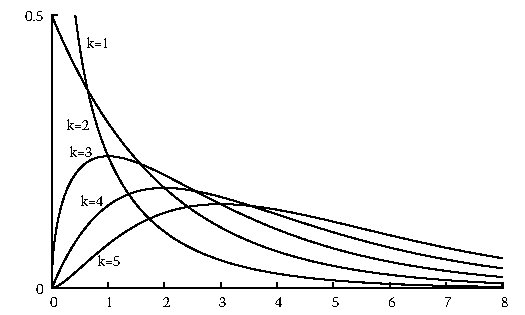
\includegraphics[width=\textwidth]{pdfChiSqr}
\end{center}
\caption[Chi-square distributions]{Chi-square distributions, $\opr{ChiSqr}(x\given k)$}
\end{figure}



\dist{Scaled chi-square} distribution~\cite{Lee2012}:
\begin{align}
\label{ScaledChiSqr}
\opr{ScaledChiSqr}(x \given \sigma, k) 
&= \frac{1}{2\sigma^2\Gamma(\tfrac{k}{2})} \Left(\frac{x}{2\sigma^2}\Right)^{\tfrac{k}{2}-1} 
\exp\Left\{-\Left(\frac{x}{2\sigma^2} \Right)\Right\} \checked \\
& \qquad \text{for positive integer } k \notag \\
&=  \opr{Stacy}(x\given 2\sigma^2, \tfrac{k}{2},1)  \checked\notag \\
&=\opr{Gamma}(x\given 0, 2\sigma^2, \tfrac{k}{2}) \checked \notag \\
&=  \opr{Amoroso}(x\given  0, 2\sigma^2, \tfrac{k}{2}, 1) \checked \notag 
\end{align}
The distribution of a sum of squares of $k$ independent normal random variables with variance $\sigma^2$.

\begin{table}[tp]
\begin{center}
\caption[Gamma distribution -- Special cases]{Special cases of the gamma family}
\label{GammaTable}
~\\
{\renewcommand{\arraystretch}{1.2} 
\begin{tabular}{llccccl}
\eqref{Gamma} & gamma & $a$ & $\theta$ & $\alpha$   \\ 
\hline
\eqref{Gamma} & Erlang & $0$ & $>\!\!0$ & $n$ \\
\eqref{StdGamma} &standard gamma & 0 & 1 & .  \\ 
\eqref{PorterThomas} & Porter-Thomas & 0 & 2 & $\tfrac{1}{2}$  \\
\eqref{ScaledChiSqr} & scaled chi-square & 0 & . & $\tfrac{1}{2}k$  \\
\eqref{ChiSqr} & chi-square & 0 & 2 & $\tfrac{1}{2}k$ \\
\eqref{Exp} & exponential & . & . & $1$  \\
\eqref{Gamma} & Wien & 0 & . & 4 \\
 \\
  & $(k,\ n\ \text{positive integers})$
 \end{tabular} 
}
\end{center}
\end{table}



\dist{Porter-Thomas} distribution~\cite{Porter1956a}:
\begin{align}
\label{PorterThomas}
\opr{PorterThomas}(x \given \sigma) 
&= \frac{1}{2\sigma^2\Gamma(\tfrac{1}{2})} \Left(\frac{x}{2\sigma^2}\Right)^{-\tfrac{1}{2}} 
\exp\Left\{-\Left(\frac{x}{2\sigma^2} \Right)\Right\} \checked \\
&=  \opr{Stacy}(x\given 2\sigma^2, \tfrac{1}{2},1)  \checked\notag \\
&=\opr{Gamma}(x\given 0, 2\sigma^2, \tfrac{1}{2}) \checked \notag \\
&=  \opr{Amoroso}(x\given  0, 2\sigma^2, \tfrac{1}{2}, 1) \checked \notag 
\end{align}
A chi-square distribution with a single degree of freedom.
Used to model fluctuations in decay mode strengths of excited nuclei~\cite{Porter1956a}.



% !TEX encoding = UTF-8 Unicode 
% !TEX root = FieldGuide.tex

\begin{table*}[tp!]

\caption[Gamma distribution -- Properties]{Properties of the gamma distribution}

\begin{align*}
\text{\hyperref[PropertiesSec]{Properties}}  \quad& \\
\text{notation} \quad &  \op{Gamma}(x\given a, \theta, \alpha) 	\checked
\\
\text{PDF} \quad &
\frac{1}{\Gamma(\alpha)\Left|\theta\Right|} 
\Left(\frac{x-a}{\theta}\Right)^{\alpha  -1}
\exp \Left\{
-  \frac{x-a}{\theta}
\Right\}
\checked \hspace{-8em}						
\\ 
\text{CDF / CCDF } \quad  &    1-Q\Left(\alpha, \tfrac{x - a }{\theta} \Right) \checked
& \theta>0 \, \big/ \,  \theta<0
\\
\text{parameters}\quad &   a,\ \theta,\ \alpha,\  \text{in } \Real, \ \alpha>0
\\
\text{support} \quad &     x \geq a &  \theta > 0
\\
&   x\leq a  &  \theta < 0 
\\
%\text{median} \quad  &  \cdots
%\\
\text{mode} \quad&   a+ \theta (\alpha-1)
& \alpha   \geq 1 \checked
\\ & a & \alpha   \le 1 \checked
\\
\text{mean} \quad& a  + \theta \alpha \checked
\\
\text{variance}  \quad&   \theta^2 \alpha \checked & 
\\
\text{skew} \quad  &  \op{sgn}(\theta)\ \frac{2}{\sqrt{\alpha}}  \checked
\\
\text{ex. kurtosis} \quad  &  \frac{6}{\alpha} \checked
\\
\text{entropy} \quad& 
\ln \bigl(|\theta| \Gamma(\alpha) \bigr)+\alpha + \Left( 1 - \alpha\Right) \psi(\alpha) \checked
\\
\text{MGF} \quad  &   e^{a t} (1- \theta t)^{-\alpha}	\checked
% Wikipedia claims restriction that I don't immediately see in other texts.
\\
\text{CF} \quad  &  e^{i a t} (1- i \theta t)^{-\alpha}		\checked
\end{align*}
\end{table*}




\SSec{Interrelations}
\label{GammaInterrelations}



Gamma distributions with common scale obey an addition property:
\begin{align*}
\opr{Gamma}_1(0, \theta, \alpha_1) +  \opr{Gamma}_2(0, \theta,\alpha_2) \sim \opr{Gamma}_3(0, \theta,\alpha_1+\alpha_2)
\checked
\end{align*}
The  sum of two independent, gamma distributed random variables (with common $\theta$'s, but possibly different $\alpha$'s) is again a gamma random variable~\cite{Johnson1994}.

The Amoroso distribution can be obtained from the standard gamma distribution by the Weibull change of variables, $x \to \Left(\tfrac{x-a}{\theta}\Right)^\beta$.
\[
\opr{Amoroso}(a ,\theta,\alpha,\beta) \sim
a+\theta \Big[{\opr{StdGamma}}(\alpha)\Big]^{1/\beta} 
\checked
\notag
\]


For large $\alpha$ the gamma distribution limits to normal~\eqref{Normal}.
\[
\opr{Normal}(x\given \mu,\sigma)   = 
\lim_{\alpha\rightarrow\infty} \opr{Gamma} (x\given  \mu- \sigma\sqrt{\alpha}, \tfrac{\sigma}{\sqrt{\alpha}}, \alpha)
\checked % Checked with MM
\notag
\]
Conversely, the sum of squares of normal distributions is a gamma distribution. See chi-square~\eqref{ChiSqr}.
\begin{align*}
\sum_{i=1,k}\oprr{StdNormal}{Normal}_i()^{2} & \sim \opr{ChiSqr}(k)  
 \sim \opr{Gamma}(0, 2,\frac{k}{2})  
 \checked
 \notag
\end{align*}



A large variety of distributions can be obtained from transformations of 1~or~2 gamma distributions, which is convenient for generating pseudo-random numbers from those distributions (See appendix~\secref{sec:random}). \label{gammatransforms}
\begin{align*}
\opr{Normal}(\mu,\sigma)   &\sim  \mu+ \sigma\ \op{Sgn}()\ \sqrt{ 2 \opr{StdGamma}(\half) } 		& \eqref{Normal}
\checked
\\
\opr{GammaExp}(a,s,\alpha) &\sim a - s \ln\bigl(\opr{StdGamma}(\alpha)\bigr) 		& \eqref{GammaExp} \checked
\\
\opr{PearsonVII}(a,s, m) & \sim a + s\ \op{Sgn}() \sqrt{ \frac{ \opr{StdGamma}_1(\half)}{\opr{StdGamma}_2(m-\half) } }		 \hspace{-1.5em}& \eqref{PearsonVII} 
\checked
% Follows since HalfPearsonVII is special case of GenBetaPrime
\\
 \opr{Cauchy}(a,s) & \sim a + s\ \op{Sgn}() \sqrt{\frac{\opr{StdGamma}_1(\half)}{\opr{StdGamma}_2(\half) } } 		& \eqref{Cauchy} \checked % Devroye1986 p445
\\
\opr{UnitGamma}(a,s,\alpha,\beta) &\sim a+ s\ \exp  \bigl(- \tfrac{1}{\beta}\opr{StdGamma}(\alpha)\bigr)		& \eqref{UnitGamma} \checked
\\
\opr{Beta}(a,s,\alpha,\gamma) & 
\sim a + s\   \Left(1 + \frac{\opr{StdGamma}_2(\gamma)}{\opr{StdGamma}_1(\alpha)} \Right)^{-1}
& \eqref{Beta} \checked 
\\
\opr{BetaPrime}(a,s,\alpha,\gamma) &\sim  a + s\ \frac{\opr{StdGamma}_1(\alpha)}{\opr{StdGamma}_2(\gamma) }		& \eqref{BetaPrime}
\checked
\\
\opr{Amoroso}(a,\theta,\alpha,\beta)&\sim a + \theta\ \opr{StdGamma}(\alpha)^{\tfrac{1}{\beta}}		& \eqref{Amoroso}
\checked
\\
\opr{BetaExp}(a,s, \alpha,\gamma)  & 
\sim a - s\ \ln   \Left(1 + \frac{\opr{StdGamma}_2(\gamma)}{\opr{StdGamma}_1(\alpha)} \Right)^{-1}	
& \eqref{BetaExp} \checked  
\\
\opr{BetaLogistic}(a,s,\alpha,\gamma) &\sim  a - s \ln \Left(\frac{\opr{StdGamma}_1(\alpha)}{\opr{StdGamma}_2(\gamma) } \Right)		& \eqref{BetaLogistic} \checked
\\
\opr{GenBeta}(a,s,\alpha,\gamma,\beta) &
 \sim a + s  \Left(1 + \frac{\opr{StdGamma}_2(\gamma)}{\opr{StdGamma}_1(\alpha)} \Right)^{-\tfrac{1}{\beta}}		& \eqref{GenBeta} \checked
\\
\opr{GenBetaPrime}(a,s,\alpha,\gamma,\beta) & \sim  a+ s \Left( \frac{\opr{StdGamma}_1(\alpha)}{\opr{StdGamma}_2(\gamma) }\Right)^{\frac{1}{\beta}}		& \eqref{GenBetaPrime}
\checked 
\end{align*}
Here, $\op{Sgn}()$ is the sign (or Rademacher) discrete random variable: 50\% chance $-1$, 50\% chance $+1$.
\index{Rademacher distribution (discrete)|see{sign distribution}}
\index{sign distribution (discrete)}



% !TEX encoding = UTF-8 Unicode 
% !TEX root = FieldGuide.tex

\Sec{Gamma-Exponential Distribution}
\label{sec:GammaExp}
\phantomsection
\addcontentsline{toc}{subsection}{~~~~~~~~~~~~Gamma-exponential} 

The {\bf gamma-exponential} (log-gamma, generalized Gompertz, generalized Gompertz-Verhulst type I, Coale-McNeil, exponential gamma) distribution \cite{Bartlett1946,Prentice1974,Johnson1995} is  a three parameter, continuous, univariate, unimodal probability density with infinite support. The functional form in the most straightforward parameterization is
\begin{align}
\label{GammaExp}
\opr{GammaExp}&(x\given \nu, \lambda, \alpha) 
\\ \notag &=
\frac{1}{ \Gamma(\alpha) |\lambda|}  \exp\Left\{- \alpha \Left(\frac{x-\nu}{\lambda}\Right) - \exp\Left(- \frac{x-\nu}{\lambda}\Right)  \Right\} \checked 
\\ \notag
& \qquad \text{for } x,\ \nu,\ \lambda,\ \alpha,\   \text{in } \mathbb{R}, 
\ \alpha>0, \ 
\\ \notag
& \qquad \text{support } -\infty \leq x \leq \infty
\notag
\end{align}
The three real parameters consist of a location parameter $\nu$, a scale parameter~$\lambda$, and a shape parameter $\alpha$. 

Note that this distribution is often called the ``log-gamma'' distribution. This naming convention is the opposite of that used for the log-normal distribution \eqref{LogNormal}. The name  ``log-gamma''  has also been used for the anti-log transform of the generalized gamma distribution, which leads to the unit-gamma distribution~\eqref{UnitGamma}.%~\cite{Gupta2004}.

%NOTE: v0.6 flipped sign of scale to make anti-log transform to gamma consistent.
Also note that the gamma-exponential is often defined with the sign of the scale $\lambda$ flipped. The parameterization used here is consistent with other log-transformed distributions. (See Log and anti-log transformation, p.\pageref{logtransform}) 



\SSec{Special cases}


\dist{Standard gamma-exponential} distribution:
\begin{align}
\label{StdGammaExp}
\opr{StdGammaExp}(x\given  \alpha) 
=&
\frac{1}{\Gamma(\alpha) }  \exp\Left\{- \alpha\, x - \exp (-x)  \Right\}  \checked
\\ \notag =& \opr{GammaExp}(x\given 0,1,\alpha) \checked
\end{align} 
The gamma-exponential distribution with zero location and unit scale.

\dist{Chi-square-exponential} (log-chi-square) distribution~\cite{Lee2012}:
\begin{align}
\label{ChiSqrExp}
\opr{ChiSqrExp}(x\given k) 
 &= \notag
\frac{1}{2^{\frac{k}{2}} \Gamma(\frac{k}{2})}  \exp\Left\{- \frac{k}{2} x - \frac{1}{2} \exp(-x)  \Right\} \checked
\\ & \qquad \text{ for positive integer } k
\\
&= \opr{GammaExp}(x\given \ln 2, 1 ,\tfrac{k}{2}) \checked
\notag
\end{align}
The log transform of the chi-square distribution~\eqref{ChiSqr}.


\dist{Generalized Gumbel} distribution~\cite{Gumbel1958,Johnson1995}: 
\begin{align}
\label{GenGumbel}
&\opr{GenGumbel}(x\given u,{\lambda},n) 
\\ \notag  &= \notag
\frac{n^n}{\Gamma(n) |{\lambda}|}  \exp\Left\{ - n \Left(\frac{x-u}{{\lambda}}\Right) - n \exp\Left(- \frac{x-u}{{\lambda}}\Right)  \Right\} \checked
\\ & \qquad \text{ for positive integer } n
\notag
\\
&= \opr{GammaExp}(x\given u-{\lambda} \ln n,{\lambda},n) \checked
\notag
\end{align}

The limiting distribution of the $n$th largest value of a large number of unbounded identically distributed random variables whose probability distribution has an exponentially decaying tail.


\begin{figure}[t]
\begin{center}
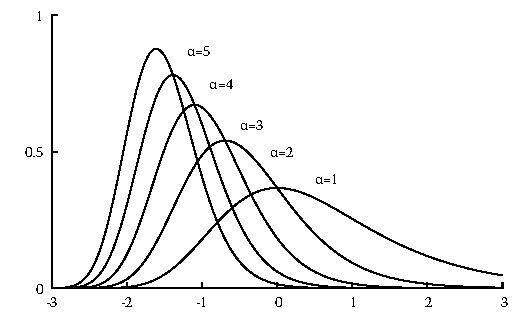
\includegraphics[width=\textwidth]{pdfGammaExp}   
\end{center}
\caption[Gamma exponential distributions]{Gamma exponential distributions, $\opr{GammaExp}(x\given 0,1,\alpha)$} 
\end{figure}


\begin{figure}[t]
\begin{center}
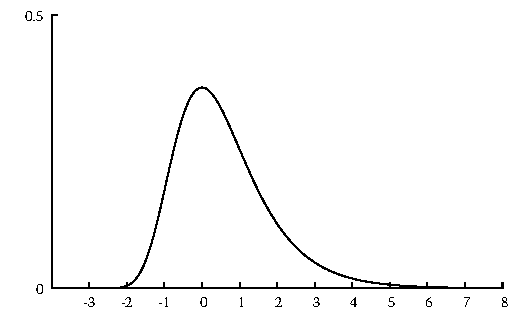
\includegraphics[width=\textwidth]{pdfGumbel}  
\end{center}
\caption[Gumbel distribution]{Standard Gumbel distribution, $\opr{StdGumbel}(x)$} 
\end{figure}


\begin{table}[tp]
\caption[Gamma-exponential distribution -- Special cases]{Special cases of the gamma-exponential family}
\begin{center}
{\renewcommand{\arraystretch}{1.25} 
\begin{tabular}{llcccl}
\eqref{GammaExp} &gamma-exponential &  $\nu$ & $\lambda$ & $\alpha$ 
\\ \hline
\eqref{StdGammaExp} & standard gamma-exponential &  $0$ & $1$ & $\alpha$  \\
\eqref{ChiSqrExp} & chi-square-exponential &$\ln 2 $ & $1$ & $\tfrac{k}{2}$ \\ 
\eqref{GenGumbel} &generalized Gumbel    & . & . & $n$ &  \\
\eqref{Gumbel} &Gumbel  &  . & . & 1 &  \\
\eqref{StdGumbel} &standard Gumbel &   0 & 1 & 1 & \\ 
\eqref{BHP} &BHP   & . & . & $\frac{\pi}{2}$ &  \\
\eqref{Moyal} & Moyal & . & . & \half 
\end{tabular}
}
\end{center}
\end{table}


% !TEX encoding = UTF-8 Unicode 
% !TEX root = FieldGuide.tex

\begin{table*}[tp!]
\caption[Gamma-exponential distribution -- Properties]{Properties of the gamma-exponential distribution}
\begin{align*}
\text{\hyperref[PropertiesSec]{Properties}}  \quad& \\
\text{notation} \quad &  \op{GammaExp}(x \given \nu, \lambda, \alpha)  			\checked
\\
\text{PDF}\quad &   \frac{1}{ \Gamma(\alpha) |\lambda|}  \exp\Left\{- \alpha \Left(\frac{x-\nu}{\lambda}\Right) - \exp\Left(-\frac{x-\nu}{\lambda}\Right)  \Right\} \checked \hspace{-8em}												
\\
\text{CDF} \big/ \text{CCDF} \quad  &   Q\Left(\alpha, e^{-\frac{x-\nu}{\lambda} }\Right) 
& \lambda>0 \ \big/ \ \lambda<0  \checked
\\
\text{parameters}\quad &   \nu,\ \lambda,\ \alpha,\   \text{in } \Real, \ \alpha>0, \ 		\checked
\\
\text{support} \quad &   x \in [-\infty, +\infty]									\checked
\\
\text{mode} \quad  & \nu -\lambda \ln \alpha \checked
\\
\text{mean} \quad  &   \nu- \lambda \psi(\alpha)	\checked
\\
\text{variance} \quad  &  \lambda^2 \psi_1(\alpha)	\checked
\\
\text{skew} \quad  &   -\text{sgn}(\lambda) \tfrac{\psi_2(\alpha) }{  \psi_1(\alpha)^{3/2} }  \checked
\\
\text{ex. kurtosis} \quad  &     \tfrac{ \psi_3(\alpha) }{  \psi_1(\alpha)^{2}} \checked
\\
%\text{entropy} \quad  &  \ln \Gamma(\alpha) |\lambda|  - \alpha \psi(\alpha) + \alpha
%\\
\text{MGF} \quad  &   e^{\nu t } \frac{\Gamma(\alpha-\lambda t)}{\Gamma(\alpha)}  \checked
& \text{\cite{Johnson1995}}  %after Eq 22.227
\\
\text{CF} \quad  &  e^{i \nu t } \frac{\Gamma(\alpha-i \lambda t)}{\Gamma(\alpha)} \checked
% Johnson1995, Eq 22.211, modulo typos
\end{align*}
\end{table*}






\dist{Gumbel}  (Fisher-Tippett type I, Fisher-Tippett-Gumbel, Gumbel-Fisher-Tippett, FTG, log-Weibull, extreme value (type I),  doubly exponential, double exponential) distribution~\cite{Fisher1928,Gumbel1958, Johnson1995}:
\begin{align}
\label{Gumbel}
\opr{Gumbel}(x\given u,{\lambda}) 
&=
\frac{1}{|{\lambda}|}  \exp\Left\{ -\Left(\frac{x-u}{{\lambda}}\Right) - \exp\Left(-\frac{x-u}{{\lambda}}\Right)  \Right\} \checked
\\
&= \opr{GammaExp}(x\given u,{\lambda},1)  \checked
\notag
\end{align}
This is the asymptotic extreme value distribution for variables of ``exponential type'', unbounded with finite moments~\cite{Gumbel1958}.
With positive scale ${\lambda}>0$, this is an extreme value distribution of the maximum, with negative scale ${\lambda}<0$ an extreme value distribution of the minimum. Note that the Gumbel is sometimes defined with the negative of the scale used here.
% Mathematica uses negative scale. Wikipedia uses this scale.

The term ``double exponential distribution'' can refer to either Laplace or Gumbel distributions~\cite{Johnson1995}.


\dist{Standard Gumbel} (Gumbel) distribution~\cite{Gumbel1958}:
\begin{align}
\label{StdGumbel}
\opr{StdGumbel}(x) 
=&
  \exp\Left\{- x - e^{-x} \Right\}  \checked \\
=& \opr{GammaExp}(x\given 0,1,1)  \notag \checked
\end{align}
The Gumbel distribution with zero location and a unit scale.



\dist{BHP} (Bramwell-Holdsworth-Pinton) distribution~\cite{Bramwell1998, Bramwell2000}:
\begin{align}
\label{BHP}
\opr{BHP}(x\given \nu,\lambda) 
&=
\frac{1}{\Gamma(\tfrac{\pi}{2}) |\lambda|}  \exp\Left\{ - \frac{\pi}{2}\Left(\frac{x-\nu}{\lambda}\Right) -  \exp\Left(-\frac{x-\nu}{\lambda}\Right)  \Right\}  \checked
\notag
\\
&= \opr{GammaExp}(x\given \nu,\lambda,\frac{\pi}{2})   \checked
\end{align}
Proposed as a model of rare fluctuations in turbulence and other correlated systems.
% v0.6 flipped sign on lambda.


\dist{Moyal} distribution~\cite{Moyal1955}:
\begin{align}
\label{Moyal}
\opr{Moyal}(x\given \mu, \lambda) & = 
\frac{1}{\sqrt{2\pi}  |\lambda|}  \exp\Left\{- \half \Left(\frac{x-\mu}{\lambda}\Right) - \half \exp\Left(- \frac{x-\mu}{\lambda}\Right)  \Right\} \checked
\\
&= \opr{GammaExp}(x\given \mu+ \lambda \ln 2, \lambda ,\half)  \checked
\notag
\end{align}
Introduced as analytic approximation to the  Landau distribution \eqref{Landau} \cite{Moyal1955}.



\SSec{Interrelations}

The name ``log-gamma'' arises because the standard log-gamma distribution is the logarithmic transform of the standard gamma distribution
\begin{align*}
\opr{StdGammaExp}(\alpha)  &\sim - \ln\Bigl( \opr{StdGamma}(\alpha) \Bigr) \checked
\\
\opr{GammaExp}(\nu, \lambda, \alpha)  &\sim -\ln\Bigl( \opr{Amoroso}(0, e^{-\nu},\alpha, \tfrac{1}{\lambda}) \Bigr) \checked
\end{align*}

The difference of two gamma-exponential distribution (with common scale) is a beta-logistic distribution \eqref{BetaLogistic}~\cite{Johnson1995}. % eq 22.212
\[
\opr{BetaLogistic}(x\given \pLoc_1-\pLoc_2,\pScale,\alpha,\gamma)   
& \sim \opr{GammaExp}_1(x\given \pLoc_1,\pScale,\alpha)  \notag \\ & \qquad -\opr{GammaExp}_2(x\given \pLoc_2,\pScale,\gamma)
\checked
\notag
\]
It follows that the difference of two Gumbel distributions \eqref{Gumbel} is a logistic distribution \eqref{Logistic}.

The gamma-exponential distribution is a limit of the Amoroso distribution \eqref{Amoroso}, and itself contains the normal \eqref{Normal} distribution as a limiting case.
\[
\lim_{\alpha\rightarrow\infty} \opr{GammaExp}(x\given  \mu+\sigma\sqrt{\alpha}\ln\alpha, \sigma\sqrt{\alpha},\alpha)
= \opr{Normal}(x\given \mu, \sigma)
\checked
\notag
\]




% !TEX encoding = UTF-8 Unicode 
% !TEX root = FieldGuide.tex

\Sec{Pearson VII Distribution}
\phantomsection\addcontentsline{toc}{subsection}{~~~~~~~~~~~~Pearson VII} 

The {\bf Pearson type VII} distribution~\cite{Pearson1916} is a three parameter, continuous, univariate, unimodal, symmetric probability distribution, with infinite support. The functional form in the most straight forward parameterization is
\begin{align}
\label{PearsonVII}
\opr{PearsonVII}(x\given a,s, m) 
%\\ \notag
&= \frac{1}{|s| B(m-\frac{1}{2}, \frac{1}{2} )} \Left( 1 +\Left( \frac{x-a}{s}\Right)^2 \Right)^{-m} 	\checked
\\ \notag
& \qquad m > \tfrac{1}{2}
\\ \notag & = \opr{PearsonIV}(x\given a,s, m,0)  \checked
\end{align}
This distribution family is notable for having long power-law tails in both directions. 


\SSec{Special cases}


\dist{Student's t} (Student, t, Student-Fisher, Fisher) distribution~\cite{Student1908,Fisher1925b,Hanley2008, Zabell2008} :
\begin{align}
\label{StudentsT}
\opr{StudentsT}(x\given k) 
&= \frac{1}{\sqrt{k} B(\frac{1}{2}, \frac{1}{2} k)} \Left( 1 + \frac{x^2}{k} \Right)^{-\frac{1}{2}(k+1)} \checked
\\ &= \opr{PearsonVII}(x\given 0,\sqrt{k},\tfrac{1}{2}(k+1)) \checked
\notag
\\ & \qquad \text{integer } k \geq 0
\notag
\end{align}
The distribution of the statistic $t$, which arises when considering the error of samples means drawn from normal random variables.
\begin{align*}
	t =& \sqrt{n} \frac {\bar{x} - \mu}{\bar{s}}  \checked \\ 
	\bar{x} & = \tfrac{1}{n} \sum_{i=1}^{n} \opr{Normal}_i (\mu,\sigma)   \checked \\
	\bar{s}^2 &= \tfrac{1}{n-1} \sum_{i=1}^{n} \bigl( \opr{Normal}_i (\mu,\sigma) - \bar{x} \bigr)^2 \checked
\end{align*}
Here, $\bar{x}$ is the sample mean of $n$ independent normal \eqref{Normal} random variables with mean $\mu$ and variance  $\sigma^2$, $\bar{s}$ is the sample variance, and $k=n-1$ is the `degrees of freedom'.


\begin{figure}[t]
\begin{center}
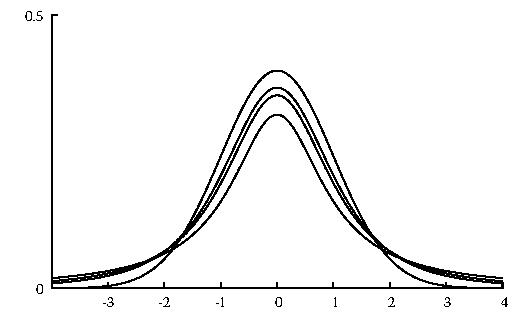
\includegraphics[width=\textwidth]{pdfStudentsT}
\end{center}
\caption[Student's t distributions]{Student's t distributions \eqref{StudentsT}: Cauchy ($k=1$), $t_2$ ($k=2$), $t_3$ ($k=3$), normal ($k\rightarrow\infty$) (low to high peak).}
\end{figure}

\begin{table*}[tp]
%\addcontentsline{toc}{subsection}{Cauchy} 
\begin{center}
\caption[Pearson VII distribution -- Special cases]{Special cases of the Pearson type VII distribution}
%\begin{align*}
%&\opr{PearsonIV}(x\given a,s, m,v) 
%\\ \notag &= \frac{{}_{2}F_1(-i\frac{v}{2}, i\frac{v}{2}, m;1)  }{s B(m-\frac{1}{2}, \frac{1}{2} )} \Left( 1 +\Left( \frac{x-a}{s}\Right)^2 \Right)^{-m}
% \exp \Left\{ - 2v \arctan \Left( \frac{x-a}{s}\Right) \Right\}
%\end{align*}
~\\
{\renewcommand{\arraystretch}{1.25}
\begin{tabular}{llcccl}
%\eqref{PearsonIV}&Pearson type IV & a & $s$ & $m$ &~$v$~ & 
\eqref{PearsonVII}&Pearson type VII & $a$ & $s$ & $m$  &  \\
 \hline
\eqref{StudentsT}& Student's $t$		& 0	& $\sqrt{k}$ & $\tfrac{k+1}{2}$  \\
\eqref{StudentsT2}& Student's $t_2$		& 0	& $\sqrt{2}$ & $\tfrac{3}{2}$  \\
\eqref{StudentsT3}& Student's $t_3$		& 0	& $\sqrt{3}$ & $2$  \\
\eqref{StudentsZ}& Student's $z$             	& 0 & 1&  n/2  \\
\eqref{Cauchy} &Cauchy 			& . & . & 1  \\
\eqref{StdCauchy} &standard Cauchy 			& 0 & 1 & 1  \\
\eqref{RelBreitWigner}& relativistic Breit-Wigner  & . & . & 2 \\
%\\
%& \underline{Limits} \\
%\eqref{Normal}& normal			& $\mu$ & $2\sigma^2 m^{\frac{1}{2}}$ & $m$ &$\lim_{m\rightarrow\infty}$ \\
\end{tabular} }
\end{center}
\end{table*}




\dist{Student's \texorpdfstring{$t_2$}{t2}} ($t_2$) distribution~\cite{Jones2002} :
\begin{align}
\label{StudentsT2}
\StudentsTT(x) 
&= \frac{1}{\Left( 2 + x^2 \Right)^{\frac{3}{2} } } \checked
\\ \notag 
& = \opr{StudentsT}(x\given 2) \checked
\\ \notag
&= \opr{PearsonVII}(x\given 0,\sqrt{2},\tfrac{3}{2}) \checked
\end{align}
Student's t distribution with 2 degrees of freedom has a particularly simple form. 

\dist{Student's \texorpdfstring{$t_3$}{t3}} ($t_3$) distribution~\cite{Devroye1986} :
\begin{align}
\label{StudentsT3}
\StudentsTTT(x)
&= \frac{2}{\pi \Left( 1 + \tfrac{x^2}{3} \Right)^{2} } \checked
\\ \notag 
& = \opr{StudentsT}(x\given 3) \checked
\\ \notag
& = \opr{RelBreitWigner}(x\given 0, \sqrt{3}, s) 
\\ \notag 
&= \opr{PearsonVII}(x\given 0,\sqrt{3},2) \checked
\end{align}
Student's t distribution with 3 degrees of freedom. Notable since the cumulative distribution function has a relatively simple form~\cite[p37]{Devroye1986}.
\[
\notag 
\op{StudentsT_3 CDF} (x) = \half + \sfrac{1}{\sqrt{3}\pi} \bigr( \arctan( \sfrac{x}{\sqrt{3}}) + \sfrac{\sfrac{x}{\sqrt{3}}}{1+\sfrac{x^2}{3}} \bigl) \checked
\]



\dist{Student's z}  distribution~\cite{Student1908,Hanley2008}:
\begin{align}
\label{StudentsZ}
\opr{StudentsZ}(z\given n) &= \frac{1}{B(\tfrac{n-1}{2}, \tfrac{1}{2})}  \Left( 1 + z^2 \Right)^{-\frac{n}{2} } \checked \\
&= \opr{PearsonVII}(z\given 0,1,\tfrac{n}{2}) \notag \checked
\end{align}
The distribution of the statistic $z$, which was the original distribution investigated by Gosset (aka Student)\footnote{Gosset's employer, the Guinness Brewing Company, insisted that he publish under a pseudonym.} in his famous 1908 paper
 on the statistical error of sample means~\cite{Student1908}.
\begin{align*}
	z &= \frac {\bar{x} - \mu}{s} \\ 
	\bar{x} &= \tfrac{1}{n} \sum_{i=1}^{n} \opr{Normal}_i (\mu,\sigma) \ , \\
	s^2 &= \tfrac{1}{n} \sum_{i=1}^{n} \bigl( \opr{Normal}_i (\mu,\sigma) - \bar{x} \bigr)^2
\end{align*}
Here, $\bar{x}$ is the sample mean of $n$ independent normal \eqref{Normal} random variables with mean $\mu$ and variance  $\sigma^2$, and $s^2$ is the sample variance, except normalized by $n$ rather than the now conventional $n-1$. Latter work by Student and Fisher~\cite{Fisher1925b} resulted in a switch to the statistic $t= z/\sqrt{n-1}$.


\dist{Cauchy} (Lorentz, Lorentzian, Cauchy-Lorentz,  Breit-Wigner, normal ratio, Witch of Agnesi) distribution~\cite{Poisson1827,Cauchy1853,Johnson1995}: 
% History see: Earliest Known Uses of Some of the Words of Mathematics
%
\begin{align}
\label{Cauchy}
\opr{Cauchy}(x\given a,s) &= \frac{1}{s \pi} \Left( 1 +\Left( \frac{x-a}{s}\Right)^2 \Right)^{-1}		\checked
\\  
&= \opr{PearsonVII}(x\given a,s,1)												\checked
\notag 
\end{align}

The Cauchy distribution is stable \eqref{Stable}\index{stable distributions}: a sum of independent Cauchy random variables is also Cauchy distributed.
\[
\opr{Cauchy}_1(a_1,s_1)  + \opr{Cauchy}_2(a_2,s_2) \sim \opr{Cauchy}_3(a_1+a_2,s_1+s_2) \checked
\notag
\]



\begin{figure}[t]
\begin{center}
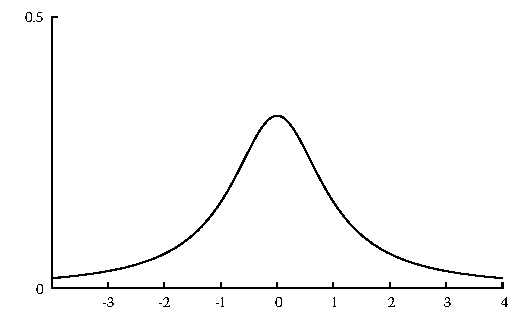
\includegraphics[width=\textwidth]{pdfCauchy}
\end{center}
\caption[Standard Cauchy distribution]{Standard Cauchy distribution, $\opr{StdCauchy}(x)$.}
\end{figure}



\dist{Standard Cauchy} distribution~\cite{Johnson1995}:
\begin{align}
\label{StdCauchy}
\opr{StdCauchy}(x) & = \frac{1}{\pi} \frac{1}{1+ x^2}				\checked
\\ 
\notag
& = \frac{1}{\pi} (x+i)^{-1} (x-i)^{-1} 							\checked
\\ \notag &= \opr{Cauchy}(x\given 0,1)						\checked
\\ \notag &= \opr{PearsonVII}(x\given 0,1,1)					\checked
\end{align}



\dist{Relativistic Breit-Wigner} (modified Lorentzian) distribution~\cite{Breit1936}:
\begin{align}
\label{RelBreitWigner}
\opr{RelBreitWigner}(x\given a, s) &= \frac{2}{ |s| \pi} \Left( 1 +\Left( \frac{x-a}{s}\Right)^2 \Right)^{-2} \checked
\\ \notag &= \opr{PearsonVII}(x\given a,s,2) \checked
\end{align}
Used to model the energy distribution of unstable particles in high-energy physics.



\SSec{Interrelations}

The Pearson VII distribution is a special case of the Pearson IV distribution~\eqref{PearsonIV}.
At high shape parameter $m$ the Pearson VII limits to the normal distribution.
\[
\opr{Normal}(x\given \mu,\sigma)   & = 
\lim_{m\rightarrow\infty} \opr{PearsonVII} ( x\given \mu, \sigma\sqrt{2m},m)
\notag
\checked
\]



The Pearson type VII distribution is given by a ratio of normal and gamma random variables
\cite[p445]{Devroye1986}.
\[
 \opr{PearsonVII}(a,s, m) \sim a+ s\sqrt{2m-1} \frac{\oprr{StdNormal}{Normal}()}{\sqrt{\opr{StdGamma}(m-\sfrac{1}{2})}} 
 \notag \checked
\]

The Cauchy distribution can be generated as a ratio of normal distributions
\[
 \opr{Cauchy}(0, 1) \sim \frac{\opr{Normal}_1(0,1)}{\opr{Normal}_2(0,1)}   \checked \notag
\]
and as a ratio of gamma distributions~\cite[p427]{Devroye1986}. %p427
\[
\Bigl(\opr{Cauchy}(0, 1)\Bigr)^2\sim  \frac{\opr{StdGamma}_1(\tfrac{1}{2})}{\opr{StdGamma}_2(\tfrac{1}{2})} 
\notag
\checked
\]




% !TEX encoding = UTF-8 Unicode 
% !TEX root = FieldGuide.tex

\begin{table*}[p]
\caption[Pearson VII distribution -- Properties]{Properties of the Pearson VII distribution}
\begin{align*}
\text{\hyperref[PropertiesSec]{Properties}}  \quad& \\
\text{notation} \quad & \text{PearsonVII}(x\given a,s, m) \checked
\\
\text{PDF}\quad &   \frac{1}{|s| B(m-\frac{1}{2}, \frac{1}{2} )} \Left( 1 +\Left( \frac{x-a}{s}\Right)^2 \Right)^{-m} \checked
\\
\text{CDF / CCDF} \quad  &  
     \frac{1}{2} +  \Left(\frac{x-a}{s}\Right) 
     \frac{1}{B(m-\frac{1}{2}, \frac{1}{2})}
     \,_2F_1 \Left ( \frac{1}{2},m;\frac{3}{2}; -\Left(\frac{x-a}{s}\Right)^2 \Right)
     \checked
     % Checked with Wolfram Alpha
     % D[1/2+ (x/s) Hypergeometric2F1[1/2, m , 3/2, -(x/s)^2] / Beta(m-1/2, 1/2), x]
     \hspace{-4em}
     \\
     &
\\
\text{parameters}\quad &   a,\ s,\ m  \in \Real \\ & m>\tfrac{1}{2} \checked
\\
\text{support} \quad &   -\infty < x < +\infty	\checked
\\
\text{median} \quad  &  a					\checked
\\
\text{mode} \quad  & a	\checked
\\
\text{mean} \quad  &  a & m>1	\checked
\\
\text{variance} \quad  & \frac{s^2}{2m-3} & m>\tfrac{3}{2} \checked
\\
\text{skew} \quad  &  0 \checked & m>2 \checked
\\
%\text{kurtosis} \quad  &  \cdots & m>\tfrac{5}{2}  
%\\ 
%\text{entropy} \quad  & \cdots
%\\
\text{MGF} \quad  &  \text{undefined}
\\
\text{CF} \quad  &   e^{iat} \frac{2 K_{m-\half} \Left( s |t|\Right)
                    \cdot \Left(\half s |t| \Right)^{m-\half}}
                    {\Gamma(m-\half)}  & m > \half
                    \checked
\end{align*}
\end{table*}




% Two shape parameter

% !TEX encoding = UTF-8 Unicode 
% !TEX root = FieldGuide.tex

\subpart{~} % To encourage page break, so that 'Two shape parameters' is at top, not bottom, of page, in table of contents.
\subpart{Two shape parameters}

\Sec{Unit Gamma Distribution} 
\label{sec:UnitGamma}
\dist{Unit gamma} (log-gamma, Grassia, log-Pearson III) distribution~\cite{Olshen1938,Consul1971,Grassia1977,Gupta2004}:
\begin{align}
\label{UnitGamma}
\opr{UnitGamma}&(x\given a, s,\alpha,\beta) \\ \notag &= \frac{1}{\Gamma(\alpha)} \Left|\frac{\beta}{ s}\Right|
\Left(\frac{x-a}{s}\Right)^{\beta-1} \Left(-\beta \ln   \frac{x-a}{s} \Right)^{\alpha-1}  \checked
\notag
\\ \text{for }& x,\ a,\ s,\ \alpha,\ \beta \text{ in } \mathbb{R},\ \ \alpha >0
\notag
 \\ \text{ support } & x \in [a,a+s], s>0,\ \beta>0 \notag \\ \text{ or } &  x\in[a+s,a], s<0,\ \beta>0 
 \notag 
 \\  \notag  \text{ or } &  x\in[a+s,+\infty], s>0,\ \beta<0 
 \\  \notag  \text{ or } &  x\in[-\infty,a+s], s<0,\ \beta<0 
\end{align}

A curious distribution that occurs as a limit of the generalized beta \eqref{GenBeta}, and as the anti-log transform of the gamma distribution \eqref{Gamma}. For this reason, it is also sometimes called the log-gamma distribution.

% Note Olsehn1938 uses parameterization with negative of beta used here.


\SSec{Special cases}


\dist{Uniform product} distribution~\cite{Springer1979a}:
\begin{align}
\label{UniformProduct}
\opr{UniformProduct}(x\given n) &=  \frac{1}{\Gamma(n)} \Left( -\ln x \Right)^{n-1} 	\checked
 \\ \notag & = \opr{UnitGamma}(x\given 0, 1,n,1)							\checked
 \\ \notag & \qquad 0>x>1, \quad n = 1,\ 2,\ 3,\ \ldots							\checked
\end{align}
The product of $n$ standard uniform distributions \eqref{StdUniform}.



\SSec{Interrelations}
With  $\alpha=1$ we obtain the power function distribution \eqref{PowerFn} as a special case.
\[
\opr{UnitGamma}(x\given a, s,1,\beta) = \opr{PowerFn}(x\given a,s,\beta) \checked \notag
\]

The  unit gamma is the anti-log transform of the standard gamma distribution \eqref{StdGamma}.
\begin{align*}
\opr{UnitGamma}(0,1,\alpha,\beta)& \sim \exp\bigl(-\opr{Gamma}(0, \tfrac{1}{\beta}, \alpha)\bigr) \checked
\\
\opr{UnitGamma}(0,1,\alpha,1) &\sim \exp\bigl(-\opr{StdGamma}( \alpha)\bigr) \checked
\end{align*}




The unit gamma distribution is a limit of the generalized beta distribution \eqref{GenBeta}, and limits to the gamma \eqref{Gamma} and log-normal  \eqref{LogNormal}~\cite{\self} distributions.
\[
\opr{Gamma}(x\given a,s,\alpha) &= \lim_{\beta\rightarrow\infty} \opr{UnitGamma}(x\given a+\beta s,-\beta s, \alpha,\beta)
\checked
\notag
\]
\begin{align*}
\lim_{\alpha\rightarrow\infty}& \opr{UnitGamma} (x\given a, \vartheta e^{ \sigma\sqrt{\alpha}}, \alpha, \tfrac{\sqrt{\alpha}}{\sigma})
\checked
\\ 
& \propto  \lim_{\alpha\rightarrow\infty}  \Left(\frac{x-a}{ \vartheta e^{ \sigma\sqrt{\alpha}} }\Right)^{ \tfrac{\sqrt{\alpha}}{\sigma} -1}
\Left(-  \frac{\sqrt{\alpha}}{\sigma} \ln  \frac{x-a}{ \vartheta e^{ \sigma\sqrt{\alpha}} } \Right)^{\alpha-1}
\checked
\\ 
& \propto  \Left(\frac{x-a}{\vartheta}\Right)^{-1}   \lim_{\alpha\rightarrow\infty}
\exp\Left\{\sqrt{\alpha}\frac{1}{\sigma} \ln \frac{x-a}{ \vartheta}\Right\}
\Left( 1 - \frac{1}{\sqrt{\alpha}} \frac{1}{\sigma} \ln  \frac{x-a}{ \vartheta  } \Right)^{\alpha-1}
\checked
\\
& \propto  \Left(\frac{x-a}{\vartheta}\Right)^{-1}   \lim_{\alpha\rightarrow\infty} e^{-z \sqrt{\alpha}}  \bigl( 1+\frac{z}{\sqrt{\alpha}} \bigr)^{\alpha} , \quad  z = -\tfrac{1}{\sigma} \ln \tfrac{x-a}{\vartheta}
\checked
\\
&  \propto \Left(\frac{x-a}{\vartheta}\Right)^{-1} \exp\Left\{-\frac{1}{2\sigma^2} \Left( \ln \frac{x-a}{\vartheta} \Right)^2 \Right\}
\checked
\\
& \quad  =  \opr{LogNormal} (x\given a, \vartheta, \sigma)
\checked
\end{align*}
\label{UnitGammaToLogNormal}
Here we utilize the Gaussian function limit $
\lim_{c \rightarrow \infty} e^{-z \sqrt{c}}  \bigl( 1+\frac{z}{\sqrt{c}} \bigr)^c = e^{-\half z^2} \checked$ \secref{sec:Limits}.
\index{Gaussian function limit}



\begin{figure}[t]
\begin{center}
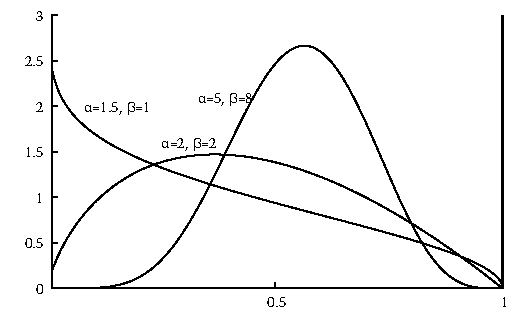
\includegraphics[width=\textwidth]{pdfUnitGamma}
\end{center}
\caption[Unit gamma, finite support.]{Unit gamma, finite support, $\opr{UnitGamma}(x\given 0, 1,\alpha,\beta)$, $\beta>0$.}
\end{figure}

\begin{figure}[t]
\begin{center}
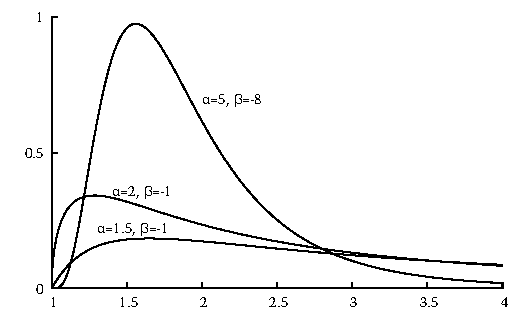
\includegraphics[width=\textwidth]{pdfUnitGammaNegBeta}
\end{center}
\caption[Unit gamma, semi-infinite support.]{Unit gamma, semi-infinite support. $\opr{UnitGamma}(x\given 0, 1,\alpha,\beta)$, $\beta<0$}
\end{figure}



The product of two unit-gamma distributions with common $\beta$ is again a unit-gamma distribution~\cite{Consul1971,\self}. 
\begin{align*}
\opr{UnitGamma}_1 (0,s_1,\alpha_1, \beta )\ & \opr{UnitGamma}_2(0,s_2, \alpha_2, \beta ) 
 \\
&\sim \opr{UnitGamma}_3(0,s_1 s_2,\alpha_1 + \alpha_2, \beta )  \checked
\end{align*}
The property is related to the  analogous additive relation of the gamma distribution.
\begin{align*}
&\opr{UnitGamma}_1(0,s_1,\alpha_1, \beta )\ \opr{UnitGamma}_2(0,s_2, \alpha_2, \beta ) 
\\
&\sim s_1 s_2 \Left(\opr{UnitGamma}_1(0,1,\alpha_1,1)\ \opr{UnitGamma}_2(0,1,\alpha_2,1)  \Right)^{\tfrac{1}{\beta}}
\\
&\sim s_1 s_2 \Left(e^{- \opr{StdGamma}_1(\alpha_1) - \opr{StdGamma}_2(\alpha_2 ) } \Right)^{ \tfrac{1}{\beta}}
\\
&\sim s_1 s_2 \Left(e^{- \opr{StdGamma}_3(\alpha_1+ \alpha_2 )  }\Right)^{\tfrac{1}{\beta}}
\\
&\sim \opr{UnitGamma}_3(0,s_1 s_2,\alpha_1 + \alpha_2, \beta ) \checked
\end{align*}



% !TEX encoding = UTF-8 Unicode 
% !TEX root = FieldGuide.tex

\begin{table*}[t!]
\caption[Unit gamma distribution -- Properties]{Properties of the unit gamma distribution}
\begin{align*}
\text{\hyperref[PropertiesSec]{Properties}}  \quad& \\
\text{notation} \quad & \text{UnitGamma}(x\given a,s,\alpha,\beta) 
\\
\text{PDF}\quad &  \frac{1}{\Gamma(\alpha)} \left|\frac{\beta}{ s}\right|
\left(\frac{x-a}{s}\right)^{\beta-1} \left(-\beta \ln   \frac{x-a}{s} \right)^{\alpha-1} \checked
\\
\text{CDF} \big/ \text{CCDF}  \quad  & 1-Q\left(\alpha, -\beta \ln \tfrac{x-a}{s} \right)
& \tfrac{\beta}{s}  >0 \ \big{/} \ \tfrac{\beta}{s}<0   \checked
\\
\text{parameters}\quad &   a, s,\alpha,\beta \text{ in } \Real  ,\  \alpha, \beta>0
\\
\text{support}\checked \quad 
	&   [a,a+s] ,\ s>0,\ \beta>0 \\
	&  [a+s,a], \ s<0,\ \beta>0 \\
	& [a+s,+\infty]  s>0,\ \beta<0  \\
 	& [-\infty,a+s], s<0,\ \beta<0 \\
%\text{median} \quad  &  \cdots
%\\
%\text{mode} \quad  & a+s \exp \left(\tfrac{1-\alpha}{1-\beta} \right)  \text{ if } \alpha,\beta>0 \text{ or } \alpha,\beta<0 \text{ (antimode)} \hspace{-4em}
%  ????
\\
\text{mean} \quad  &  a + s \left(\tfrac{\beta}{\beta+1} \right)^{\alpha} \checked
\\
\text{variance} \quad  & s^2 \left(\tfrac{\beta}{\beta+2} \right)^{\alpha} - s^2 \left(\tfrac{\beta}{\beta+1} \right)^{2\alpha} \checked
\\
\text{skew} \quad  &   \text{not simple}
\\
\text{kurtosis} \quad  &   \text{not simple}
\\
\text{entropy} \quad  & \cdots
\\
\text{MGF} \quad  &  \cdots
\\
\text{CF} \quad  &  \cdots
\\
E(X^h) \quad & \left(\tfrac{\beta}{\beta+h} \right)^{\alpha} \qquad  & a=0 \
\text{\cite{Grassia1977}} \checked
\end{align*}
\end{table*}



% !TEX encoding = UTF-8 Unicode 
% !TEX root = FieldGuide.tex

\Sec{Amoroso Distribution}
\label{sec:Amoroso}
\phantomsection\addcontentsline{toc}{subsection}{~~~~~~~~~~~~Amoroso} 
The {\bf Amoroso}  (generalized gamma, Stacy-Mihram) distribution~\cite{Amoroso1925,Johnson1994,Gonzalez2013} is a four parameter,  continuous, univariate, unimodal probability density, with semi-infinite support. The functional form in the most straightforward parameterization is
\begin{align}
\label{Amoroso}  
 \opr{Amoroso}(x&\given  a, \theta, \alpha, \beta) 
\\ \notag&=
\frac{1}{\Gamma(\alpha)} 
\left|\frac{\beta}{\theta}\right|
\left(\frac{x-a}{\theta}\right)^{\alpha \beta -1}
\exp \left\{
-  \left(\frac{x-a}{\theta}\right)^{\beta}
\right\}
\checked
\\ \notag
& \text{for } x,\ a,\ \theta,\ \alpha,\ \beta\  \text{in } \mathbb{R}, 
\ \alpha>0, \ 
\\ \notag
& \text{support } x \geq a \ \text{if}\ \theta > 0,  \ x\leq a  \ \text{if}\  \theta < 0 .
\end{align}

The Amoroso distribution was originally developed to model lifetimes \cite{Amoroso1925}. It occurs as the Weibullization of the standard gamma distribution \eqref{Gamma} and, with integer $\alpha$, in extreme value statistics \eqref{GenFisherTippett}. The Amoroso distribution is itself a limiting form of various more general distributions, most notable the generalized beta \eqref{GenBeta} and generalized beta prime \eqref{GenBetaPrime} distributions~\cite{McDonald1984}.
Many common and interesting probability distributions are special cases or limiting forms of the Amoroso  (See Table~\ref{AmorosoTable}). 


The four real parameters of the Amoroso distribution consist of a location parameter~$a$, 
a scale parameter~$\theta$,  and two shape parameters,~$\alpha$ and~$\beta$. Whenever these symbols appears in special cases or limiting forms, they refer directly to the parameters of the Amoroso distribution.
The shape parameter $\alpha$ is positive, and in many special cases an integer, $\alpha=n$, or half-integer, $\alpha=\tfrac{k}{2}$. The negation of a standard parameter is indicated by a bar, e.g.\ $\bar{\beta} = -\beta$. The chi, chi-squared and related distributions are traditionally parameterized with the scale parameter $\sigma$, where $\theta= (2\sigma^2)^{1/{\beta}}$, and $\sigma$ is the standard deviation of a related normal distribution.  Additional alternative parameters are introduced as necessary. 
  


\begin{table*}[p]
\begin{center}
\label{AmorosoTable}
\caption[Amoroso and gamma distributions -- Special cases]{Special cases of the Amoroso and gamma families}
~\\
{\renewcommand{\arraystretch}{1.1} 
\begin{tabular}{llccccl}
\eqref{Amoroso} &Amoroso & $a$ & $\theta$ & $\alpha$ & $\beta$
\\ \hline
\eqref{Stacy} & Stacy & $0$ & . & . & . \\
\eqref{HalfExpPower} & half exponential power & . & . & $\tfrac{1}{\beta}$ & . \\
\eqref{GenFisherTippett} & gen. Fisher-Tippett  & . & . & $n$ & .  \\
\eqref{FisherTippett} &  Fisher-Tippett & . & . & 1 & .  \\
\eqref{Frechet} &Fr\'{e}chet  & . & . & 1 &  $<\!\!0$  \\
\eqref{GenFrechet} &  generalized Fr\'{e}chet & . & . & $n$ & $<\!\!0$ \\
\eqref{ScaledInvChi} &scaled inverse chi& 0 & . & $\tfrac{1}{2}k$  & -2  \\
\eqref{InvChi} & inverse chi  & 0 & $\frac{1}{\sqrt{2}}$ & $\tfrac{1}{2}k$ & -2 \\
\eqref{InvRayleigh} &  inverse Rayleigh  & $0$ & . & $1$ & -2 \\
\eqref{InvGamma} & inverse gamma & . & . & . & -1 \\
\eqref{ScaledInvChiSqr} & scaled inverse chi-square & 0 & . & $\tfrac{1}{2}k$ & -1 \\
\eqref{InvChiSqr} & inverse chi-square & 0 & $\frac{1}{2}$ & $\tfrac{1}{2}k$ & -1 \\
\eqref{Levy} & L\'{e}vy &  . & . & $\frac{1}{2}$ & -1 \\
\eqref{InvExp} &  inverse exponential & 0  & . & 1 & -1 \\
\eqref{Gamma} &gamma & . & . & . & $1$ \\
\eqref{Gamma} & Erlang & $0$ & $>\!\!0$ & $n$ & $1$ \\
\eqref{StdGamma} &standard gamma & 0 & 1 & . & 1  \\ 
\eqref{PorterThomas} & Porter-Thomas & 0 & 2 & $\tfrac{1}{2}$ & 1 \\
\eqref{ScaledChiSqr} & scaled chi-square & 0 & . & $\tfrac{1}{2}k$ & 1 \\
\eqref{ChiSqr} & chi-square & 0 & 2 & $\tfrac{1}{2}k$ & 1 \\
\eqref{Exp} & exponential & . & . & $1$ & $1$ \\
\eqref{Gamma} & Wien & 0 & . & 4& 1 \\
\eqref{Hohlfeld} & Hohlfeld & 0 & . & $\tfrac{2}{3}$ & $\tfrac{3}{2}$ \\
\eqref{Nakagami} & Nakagami & . & . & . & $2$ \\
\eqref{ScaledChi} &scaled chi& 0 & . & $\tfrac{1}{2}k$  & 2  \\
\eqref{Chi} & chi & 0 & $\sqrt{2}$ & $\tfrac{1}{2}k$ & 2 \\
\eqref{HalfNormal} & half normal & 0 & . & $\tfrac{1}{2}$ & 2 & \\  
\eqref{Rayleigh} & Rayleigh & 0 & . & 1 & 2  \\
\eqref{Maxwell} & Maxwell& 0 & . & $\frac{3}{2}$  & 2  \\
\eqref{WilsonHilferty} &Wilson-Hilferty& 0 & . & .  & 3  \\
\eqref{GenWeibull} & generalized Weibull  & . & . & $n$ & $>\!\!0$  \\
\eqref{Weibull} & Weibull & . & . & 1 &  $>\!\!0$  \\
\eqref{PseudoWeibull} & pseudo-Weibull & . & . & $1$+$\tfrac{1}{\beta}$ &  $>\!\!0$  \\
\\
& $(k,\ n\ \text{positive integers})$
\end{tabular} 
}
\end{center}
\end{table*}



\SSec{Special cases: Miscellaneous}

The gamma distribution ($\beta=1$) and it's special cases are detailed in \secref{sec:Gamma}.

\dist{Stacy} (hyper gamma, generalized Weibull, Nukiyama-Tanasawa, generalized gamma, generalized semi-normal, hydrograph, Leonard hydrograph, transformed gamma)  distribution~\cite{Stacy1962,Dadpay2007}:
\begin{align}
\label{Stacy}
\opr{Stacy}(x \given \theta, \alpha, \beta) 
=& \frac{1}{\Gamma(\alpha)} \left|\frac{\beta}{\theta}\right| \left(\frac{x}{\theta}\right)^{\alpha\beta-1} 
\exp \left\{ -\left(\frac{x}{\theta}\right)^{\beta} \right\} \checked
\\=&  \opr{Amoroso}(x\given  0, \theta, \alpha, \beta) \notag \checked
\end{align}
If we drop the location parameter from $\opr{Amoroso}$, then we obtain the 
Stacy, or generalized gamma distribution, the parent of the gamma family of distributions.
If $\beta$ is negative then the distribution is  {\bf generalized inverse gamma}, the parent of various inverse distributions, including the inverse gamma \eqref{InvGamma} and inverse chi \eqref{InvChi}. 

The Stacy distribution is obtained as the positive even powers,  modulus, and powers of the modulus of a centered, normal random variable \eqref{Normal}, 
\[
\opr{Stacy}\left((2\sigma^2)^{\tfrac{1}{\beta}} ,\tfrac{1}{2}, \beta\right) \sim \Big|\opr{Normal}(0,\sigma)\Big|^{\tfrac{2}{\beta}}
\notag
\checked
\]
and as powers of the sum of squares of $k$ centered, normal random variables. 
\[
\opr{Stacy}\left( (2\sigma^2)^{\tfrac{1}{\beta}} ,\tfrac{1}{2}k, \beta\right) \sim  \left( \sum_{i=1}^{k} \Bigl(\opr{Normal}(0,\sigma)\Bigr)^2\right)^{\tfrac{1}{\beta}}
\notag
\checked
\]



\dist{Pseudo-Weibull} distribution~\cite{Voda1989}:
\begin{align}
\label{PseudoWeibull}
\opr{PseudoWeibull}(x\given a, \theta,\beta)  
=& \frac{1}{\Gamma(1+\tfrac{1}{\beta})} \frac{\beta}{|\theta|} \left(\frac{x-a}{\theta}\right)^{\beta} 
\exp \left\{ -\left(\frac{x-a}{\theta}\right)^{\beta} \right\} \checked
\\ & \text{for } \beta>0 \notag 
\\=&  \opr{Amoroso}(x\given  a, \theta, 1+\tfrac{1}{\beta}, \beta) \notag \checked
\end{align}
Proposed as another model of failure times. 

\dist{Half exponential power} (half Subbotin) distribution~\cite{Gui2013}:
\begin{align}
\label{HalfExpPower}
\opr{HalfExpPower}(x\given a, \theta,\beta)
=& 
\frac{1}{\Gamma(\tfrac{1}{\beta})} 
\left|\frac{\beta}{\theta}\right|
\exp \left\{
-  \left(\frac{x-a}{\theta}\right)^{\beta}
\right\} \checked
\\=&  \opr{Amoroso}(x\given  a, \theta,\tfrac{1}{\beta}, \beta) \notag \checked
\end{align}
As the name implies, half an exponential power \eqref{ExpPower} distribution. Special cases include $\beta=-1$ inverse exponential  \eqref{InvExp}, $\beta=1$ exponential \eqref{Exp}, $\beta=\tfrac{2}{3}$ Hohlfeld  \eqref{Hohlfeld}  and $\beta=2$ half normal \eqref{HalfNormal} distributions. 

\dist{Hohlfeld} distribution~\cite{Hohlfeld2014}:
\begin{align}
\label{Hohlfeld}
\opr{Hohlfeld}(x\given a, \theta)
=& 
\frac{1}{\Gamma(\tfrac{2}{3})} 
\left|\frac{3}{2\theta}\right|
\exp \left\{
-  \left(\frac{x-a}{\theta}\right)^{3/2}
\right\} \checked
\\=&  \opr{HalfExpPower}(x\given a, \theta,\tfrac{3}{2}) \notag \checked
\\=&  \opr{Amoroso}(x\given  a, \theta,\tfrac{2}{3}, \tfrac{3}{2}) \notag \checked
\end{align}
Occurs in the extreme statistics of Brownian ratchets  \cite[Suppl. p.5]{Hohlfeld2014}.





% ========================================================================
\SSec{Special cases: Positive integer \texorpdfstring{$\beta$}{beta}}

\begin{figure}[t]
\begin{center}
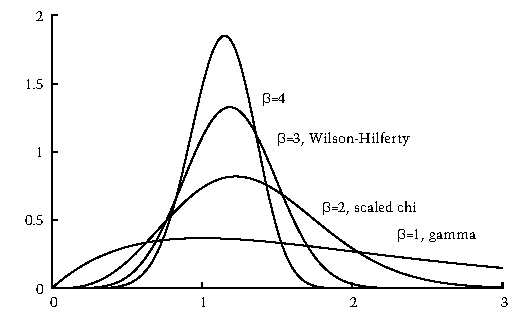
\includegraphics[width=\textwidth]{pdfAmorosoBetaPDF}
\end{center}
\caption[Gamma, scaled chi and Wilson-Hilferty distributions]{Gamma, scaled chi and Wilson-Hilferty distributions, $\opr{Amoroso}(x\given 0,1,2,\beta)$}
\end{figure}

With $\beta=1$ we obtain the gamma family of distributions: gamma \eqref{Gamma}, standard gamma \eqref{StdGamma} and chi square \eqref{ChiSqr} distributions. See \secref{sec:Gamma}.



\dist{Nakagami} (generalized normal, Nakagami-m, m) distribution~\cite{Nakagami1960}:
\begin{align}
\label{Nakagami}
 \opr{Nakagami}&(x \given a , \theta, \alpha) 
\\ \notag 
& =
 \frac{2}{\Gamma(\alpha) |\theta| }
\left(\frac{x-a }{\theta}\right)^{2\alpha -1}
\exp \left\{
-  \left(\frac{x-a }{\theta}\right)^{2}
\right\}
\checked
\\ \notag
& = \opr{Amoroso}(x\given a,\theta, \alpha ,2) \checked
\notag
\end{align}
Used to model attenuation of radio signals that reach a receiver by multiple paths~\cite{Nakagami1960}.




\dist{Half normal} (semi-normal, positive definite normal, one-sided normal) distribution~\cite{Johnson1994}:
%
\begin{align}
\label{HalfNormal}
\opr{HalfNormal}(x \given a, \sigma ) 
&= \frac{2}{\sqrt{2\pi \sigma^2}} 
\exp\left\{-\left( \frac{(x-a)^2}{2\sigma^2}\right) \right\}  
\checked
\\
& \qquad (x-a)/\sigma>0 \notag \\
%&=\opr{ScaledChi}(x \given  \sigma, 1) \notag \checked \\
%&=  \opr{Stacy}(x\given  \sqrt{2\sigma^2} ,\tfrac{1}{2},2) \notag \checked \\
&=  \opr{Amoroso}(x\given  a, \sqrt{2\sigma^2} , \tfrac{1}{2}, 2) \notag  \checked
\end{align}
The modulus of a normal distribution about the mean.

\dist{Chi} ($\chi$) distribution~\cite{Johnson1994}:
%
\begin{align}
\label{Chi}
\opr{Chi}(x \given k) 
&= \frac{ \sqrt{2}}{\Gamma(\tfrac{k}{2})} { \left(\frac{x}{\sqrt{2}}\right)}^{k-1} 
\exp\left\{ -\left( \frac{x^2}{2}    \right)\right\} \checked
\\
& \qquad \text{for positive integer } k \notag \\
& = \opr{ScaledChi}(x\given 1,k) \notag \checked \\
&=  \opr{Stacy}(x\given \sqrt{2}, \sfrac{k}{2}, 2)  \notag \checked \\
&=  \opr{Amoroso}(x\given  0, \sqrt{2} , \sfrac{k}{2}, 2) \notag \checked
\end{align}
The root-mean-square of $k$ independent standard normal variables, or the square root of a chi-square random variable.
\[
\opr{Chi}(k) \sim \sqrt{\opr{ChiSqr}(k)} \checked
\notag
\]

\dist{Scaled chi} (generalized Rayleigh) distribution~\cite{Miller1964,Johnson1994}:
\begin{align}
\opr{ScaledChi}(x \given \sigma, k) 
&= \frac{2}{\Gamma(\tfrac{k}{2}) \sqrt{2\sigma^2}} { \left(\frac{x}{\sqrt{2\sigma^2}}\right)}^{k-1} 
\exp\left\{-\left(\frac{x^2}{2\sigma^2}\right)\right\} 
\notag \checked
\\
& \qquad \text{for positive integer } k \notag \checked \\
&=  \opr{Stacy}(x\given \sqrt{2\sigma^2}, \tfrac{k}{2},2)  \checked
\label{ScaledChi}
\\
&=  \opr{Amoroso}(x \given 0, \sqrt{2\sigma^2}, \tfrac{k}{2}, 2) \checked
\notag 
\end{align}
The root-mean-square of $k$ independent and identically distributed normal variables with zero mean and variance~$\sigma^2$. 


\begin{figure}[t]
\begin{center}
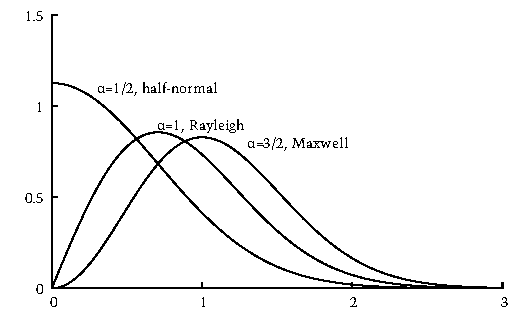
\includegraphics[width=\textwidth]{pdfAmorosoBeta2PDF}
\end{center}
\caption[Half normal, Rayleigh and Maxwell distributions]{Half normal, Rayleigh and Maxwell distributions, $\opr{Amoroso}(x\given 0,1,\alpha,2)$}
\end{figure}



\dist{Rayleigh} (circular normal) distribution~\cite{Strutt1880,Johnson1994}:
%
\begin{align}
\label{Rayleigh}
\opr{Rayleigh}(x \given \sigma) 
&= \frac{1}{\sigma^2 }\ x\  \exp\left\{-\left(\frac{x^2}{2 \sigma^2}\right)\right\}  \checked
\\
&=\opr{ScaledChi}(x \given \sigma, 2) \notag 							\checked \\
&=  \opr{Stacy}(x\given  \sqrt{2\sigma^2} ,1,2) \notag					\checked \\
&=  \opr{Amoroso}(x\given  0, \sqrt{2\sigma^2} , 1, 2) 					\checked \notag 
\end{align}
 The root-mean-square of two independent and identically distributed normal variables with zero mean and variance $\sigma^2$. 
 For instance, wind speeds are approximately Rayleigh distributed, since the horizontal components of the velocity are approximately normal, and the vertical component is typically small~\cite{Justus1978}. 


\dist{Maxwell} (Maxwell-Boltzmann, Maxwell speed, spherical normal) distribution~\cite{Maxwell1860, Abramowitz1965}:
%
\begin{align}
\label{Maxwell}
\opr{Maxwell}(x \given \sigma) 
&= \frac{\sqrt{2}}{\sqrt{\pi} \sigma^3}\ x^2 \exp\left\{-\left(\frac{x^2}{2\sigma^2}\right)\right\}  \checked
 \\
%& x>0,   \notag \\
&=\opr{ScaledChi}(x \given \sigma, 3) \checked \notag \\
&=  \opr{Stacy}(x\given  \sqrt{2\sigma^2} ,\tfrac{3}{2},2) \notag  \checked\\
&=  \opr{Amoroso}(x\given  0, \sqrt{2\sigma^2} , \tfrac{3}{2}, 2) \notag  \checked
\end{align}
The speed distribution of molecules in thermal equilibrium. The root-mean-square of three independent and identically distributed normal variables with zero mean and variance $\sigma^2$.



\dist{Wilson-Hilferty} distribution~\cite{Wilson1931,Johnson1994}:
\begin{align}
\label{WilsonHilferty}
\opr{WilsonHilferty}(x \given \theta, \alpha) 
&= \frac{3}{\Gamma(\alpha)|\theta|} \left(\frac{x}{\theta}\right)^{3 \alpha-1} \exp\left\{-\left(\frac{x}{\theta}\right)^{3}\right\}
\checked
\\ 
&=  \opr{Stacy}(x\given \theta, \alpha, 3) \checked
\notag 
\\ &=  \opr{Amoroso}(x\given  0, \theta, \alpha, 3) \checked
\notag
\end{align}
The cube root of a gamma variable follows the Wilson-Hilferty distribution~\cite{Wilson1931}, which has been used to approximate a normal distribution if $\alpha$ is not too small.
\[
\opr{WilsonHilferty}(x \given \theta, \alpha)  \approx \opr{Normal}(x \given 1-\sfrac{2}{9\alpha},  \sfrac{2}{9\alpha} )
\checked
\notag
\]


A related approximation using quartic roots of gamma variables~\cite{Hawkins1986} leads to   $\opr{Amoroso}(x\given  0, \theta, \alpha, 4)$.


% ====================================================================

\SSec{Special cases: Negative integer \texorpdfstring{$\beta$}{beta}}


With negative $\beta$ we obtain various ``inverse'' distributions related to distributions with positive $\beta$ by the reciprocal transformation $ (\tfrac{x-a}{\theta} ) \mapsto (\tfrac{\theta}{x-a} )$.



\dist{Inverse gamma} (Pearson type V, March, Vinci) distribution~\cite{Pearson1901, Johnson1994}:
\begin{align}
\label{InvGamma}
\opr{InvGamma}(x \given \theta, \alpha) 
&= \frac{1}{\Gamma(\alpha) |\theta|} \left(\frac{\theta}{x-a}\right)^{\alpha+1} 
 \exp\left\{-\left( \frac{\theta}{x-a}   \right)\right\}  \checked
\\
%& = \opr{PearsonV}(x\given a,\theta,\alpha)  \notag \checked \\
&=  \opr{Amoroso}(x\given  a, \theta, \alpha, -1) \notag  \checked
\end{align}
Occurs as the conjugate prior for an exponential distribution's scale parameter~\cite{Johnson1994}, or the prior for variance of a  normal distribution with known mean~\cite{Gelman2004}. Frequently defined with zero scale parameter.


\dist{Inverse exponential} distribution~\cite{Kleiber2003}:
\begin{align}
\label{InvExp}
\opr{InvExp}(x \given a, \theta) 
&= \frac{1}{|\theta|} \left(\frac{\theta}{x-a }\right)^2  \exp\left\{-\left( \frac{\theta}{x-a}   \right)\right\}   \checked \\
&=  \opr{InvGamma}(x\given a,  \theta, 1)  \checked \notag \\
&=  \opr{Amoroso}(x\given  a, \theta, 1, -1) \checked \notag 
\end{align}
Note that the name ``inverse exponential'' is occasionally used for the ordinary exponential distribution \eqref{Exp}.


\begin{figure}[t]
\begin{center}
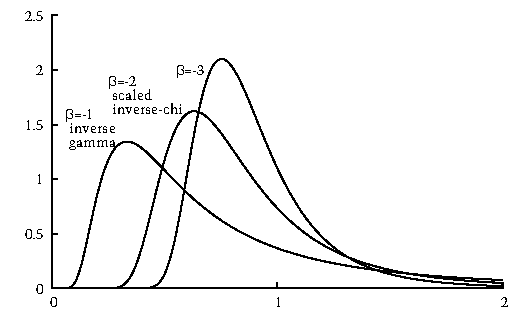
\includegraphics[width=\textwidth]{pdfAmorosoBetaNegPDF}
\end{center}
\caption[Inverse gamma and scaled inverse-chi distributions]{Inverse gamma and scaled inverse-chi distributions, $\opr{Amoroso}(x\given 0,1,2,\beta)$, negative $\beta$.}
\end{figure}




% ===============================
\dist{L\'{e}vy} distribution (van der Waals profile)~\cite{Feller1971}: 
\begin{align}
\label{Levy}
\Levy(x \given a, c) 
&= \sqrt{\frac{|c|}{2\pi}} \frac{1}{(x-a)^{3/2}}  \exp\left\{-\frac{c}{2(x-a)}\right\}  \checked
\\
%&= \opr{PearsonV}(x\given a,\tfrac{c}{2},\tfrac{1}{2})  \checked\notag \\
&=  \opr{Amoroso}(x\given  a, \tfrac{c}{2}, \tfrac{1}{2}, -1) \checked \notag 
\end{align}
The L\'{e}vy distribution is notable for being stable\index{stable distributions}:  a linear combination of identically distributed  L\'{e}vy distributions is again a  L\'{e}vy distribution. The other stable distributions with analytic forms are the normal distribution \eqref{Normal}, which is also a limit of the Amoroso distribution, and the Cauchy distribution \eqref{Cauchy}, which is not. L\'{e}vy distributions describe first passage times in one dimension~\cite{Feller1971}. See also the inverse Gaussian distribution \eqref{InvGaussian}, the  first passage time distribution for Brownian diffusion with drift.
\index{first passage time}
\index{diffusion}


\dist{Scaled inverse chi-square}  distribution~\cite{Gelman2004}:
\begin{align}
\label{ScaledInvChiSqr}
\opr{ScaledInvChiSqr}&(x \given \sigma, k) 
\\ \notag =& \frac{2 \sigma^2}{\Gamma(\tfrac{k}{2}) } \left(\frac{1}{2 \sigma^2x}\right)^{\frac{k}{2}+1} 
\exp\left\{-\left( \frac{1}{2 \sigma^2x}   \right)\right\} \checked
\\
&\qquad  \text{for positive integer } k \notag \\
&=  \opr{InvGamma}(x\given 0, \tfrac{1}{2 \sigma^2}, \tfrac{k}{2}) \notag  \checked \\
%&= \opr{PearsonV}(x\given 0,\tfrac{1}{2 \sigma ^2},\tfrac{k}{2})  \notag  \checked \\
&= \opr{Stacy}(x\given  \tfrac{1}{2 \sigma ^2},\tfrac{k}{2}, -1)  \notag  \checked \\
&=  \opr{Amoroso}(x\given  0, \tfrac{1}{2 \sigma ^2}, \tfrac{k}{2}, -1) \checked \notag 
\end{align}
A special case of the inverse gamma distribution with half-integer $\alpha$. Used as a prior for variance parameters in normal models~\cite{Gelman2004}.




\dist{Inverse chi-square} distribution~\cite{Gelman2004}: 
%
\begin{align}
\label{InvChiSqr}
\opr{InvChiSqr}(x \given k) 
=& \frac{2}{\Gamma(\tfrac{k}{2}) } \left(\frac{1}{2x}\right)^{\frac{k}{2}+1} \exp\left\{-\left( \frac{1}{2x}  \right)\right\}
\checked  \\
&\qquad  \text{for positive integer } k \notag \\
& = \opr{ScaledInvChiSqr}(x\given 1,k)\notag \checked \\
&=  \opr{InvGamma}(x\given 0, \tfrac{1}{2}, \tfrac{k}{2}) \notag \checked \\
%&= \opr{PearsonV}(x\given 0,\tfrac{1}{2},\tfrac{k}{2})  \notag \checked \\
&=  \opr{Stacy}(x\given \tfrac{1}{2}, \tfrac{k}{2},-1) \notag  \checked\\
&=  \opr{Amoroso}(x\given  0, \tfrac{1}{2}, \tfrac{k}{2}, -1)  \checked\notag 
\end{align}
A standard scaled inverse chi-square distribution.



\dist{Scaled inverse chi} distribution~\cite{Lee2012}:
\begin{align}
\label{ScaledInvChi}
 \opr{ScaledInvChi}&(x \given \sigma, k) 
\\ \notag
&= \frac{2 \sqrt{2 \sigma ^2} }{ \Gamma(\tfrac{k}{2})} { \left(\frac{1}{\sqrt{2 \sigma^2} x}\right)}^{k+1} \exp\left\{-\left(\frac{1}{2 \sigma^2 x^2}  \right)\right\} \checked
\\
&=  \opr{Stacy}(x\given \tfrac{1}{\sqrt{2 \sigma^2}}, \tfrac{k}{2}, -2)  \notag \checked \\
&=  \opr{Amoroso}(x\given  0, \tfrac{1}{\sqrt{2 \sigma^2}}, \tfrac{k}{2}, -2) \notag  \checked
\end{align}
Used as a prior for the standard deviation of a normal distribution.

\dist{Inverse chi} distribution~\cite{Lee2012}: 
\begin{align}
\label{InvChi}
\opr{InvChi}(x \given k) 
&= \frac{2\sqrt{2} }{ \Gamma(\tfrac{k}{2})} { \left(\frac{1}{\sqrt{2} x}\right)}^{k+1} \exp\left\{-\left(\frac{1}{2 x^2}  \right)\right\}
\checked
\\
&=  \opr{Stacy}(x\given  \tfrac{1}{\sqrt{2}}, \tfrac{k}{2}, -2)  \notag \checked \\
&=  \opr{Amoroso}(x\given  0, \tfrac{1}{\sqrt{2}} , \tfrac{k}{2}, -2) \notag  \checked
\end{align}


\dist{Inverse Rayleigh} distribution~\cite{Evans2000}:
\begin{align}
\label{InvRayleigh}
\opr{InvRayleigh}(x \given \sigma) 
&= 2 \sqrt{2 \sigma ^2}    \left(\frac{1}{\sqrt{2 \sigma^2} x}\right)^{3} \exp\left\{-\left(\frac{1}{2 \sigma^2 x^2}  \right)\right\}
\checked
\\
&=  \opr{Stacy}(x\given \tfrac{1}{\sqrt{2 \sigma^2}}, 1, -2)  \notag \checked \\
& = \Frechet(x\given 0, \tfrac{1}{\sqrt{2 \sigma^2}}, 2)\notag \\
&=  \opr{Amoroso}(x\given  0, \tfrac{1}{\sqrt{2 \sigma^2}}, 1, -2)  \checked \notag 
\end{align}
The inverse Rayleigh distribution has been used to model  failure time~\cite{Voda1972}.


% ====================================================================



\SSec{Special cases: Extreme order statistics}
\label{SecExtremeOrderStatistic}
\index{extreme order statistics}


\begin{figure}[t]
\begin{center}
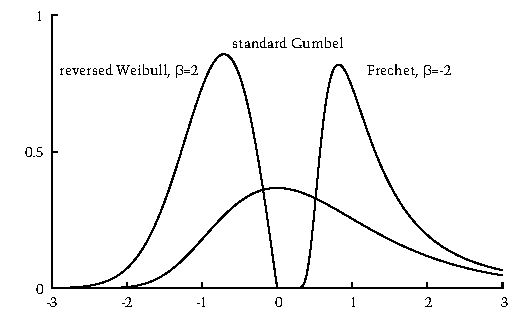
\includegraphics[width=\textwidth]{pdfEVD}
\end{center}
\caption{Extreme value distributions of maxima.}
\end{figure}



\dist{Generalized Fisher-Tippett} distribution~\cite{Smirnov1949,Barndorff-Nielsen1963}:
\begin{align}
\label{GenFisherTippett}  
 \opr{GenFisherTippett}&(x\given  a, \omega, n, \beta) 
\notag
\\ \notag
&=
\frac{n^n}{\Gamma(n)} 
\left|\frac{\beta}{\omega}\right|
\left(\frac{x-a}{\omega}\right)^{n \beta -1}
\exp \left\{
-  n \left(\frac{x-a}{\omega}\right)^{\beta}
\right\} \checked
\\
& \quad \text{for positive integer } n
\\ \notag
& = \opr{Amoroso}(x\given a,{\omega}/{n^{\frac{1}{\beta} }},n,\beta) \checked
\end{align}
If we take $N$ samples from a probability distribution, then asymptotically for large $N$ and $n\ll N$, the distribution of the $n$th largest (or smallest) sample follows a generalized Fisher-Tippett distribution. The parameter $\beta$ depends on the tail behavior of the sampled distribution. Roughly speaking, if the tail is unbounded and decays exponentially then $\beta$ limits to $\infty$, if the tail scales as a power law then $\beta<0$,  and if the tail is finite $\beta>0$~\cite{Gumbel1958}. In these three limits we obtain the Gumbel (\ref{Gumbel}, \ref{GenGumbel}), Fr\'{e}chet (\ref{Frechet}, \ref{GenFrechet}) and Weibull (\ref{Weibull},\ref{GenWeibull}) families of extreme value distribution (Extreme value distributions types I, II and III) respectively. If $\beta/\omega$ is negative we obtain distributions for the $n$th maxima, if positive then the $n$th minima.

% According to wikipedia, McFadden first wrote down unifying form of GEV.

\dist{Fisher-Tippett} (Generalized extreme value, GEV, von Mises-Jenkinson, von Mises extreme value, log-Gumbel, Brody) distribution~\cite{Fisher1928, Mises1936, Gumbel1958,Johnson1995,McFadden1978a}:
\begin{align}
\label{FisherTippett}
\opr{FisherTippett}&(x\given  a , \omega, \beta) 
\\ \notag
&=
\left|\frac{\beta}{\omega}\right|
\left(\frac{x-a}{\omega}\right)^{ \beta -1}
\exp \left\{
-  \left(\frac{x-a}{\omega}\right)^{\beta} 
\right\} \checked
\\ \notag & = \opr{GenFisherTippett}(x\given a, \omega, 1, \beta) \checked
\\ \notag & = \opr{Amoroso}(x\given a, \omega, 1, \beta) \checked
\end{align}
The asymptotic distribution of the extreme value from a large sample. The superclass of type I, II and III (Gumbel, Fr\'{e}chet, Weibull) extreme value distributions~\cite{Mises1936}.  This is the {\bf max stable distribution} (distribution of maxima) with $\beta/\omega<0$ and the {\bf min stable distribution}  (distribution of minima) for $\beta/\omega>0$.


The maximum of two Fisher-Tippett random variables (minimum if $\beta/\omega>0$)  is again a Fisher-Tippett random variable. 
\begin{align*}
\max\Big[ \opr{FisherTippett}(a,\omega_1,\beta),  \opr{FisherTippett}(a, \omega_2,\beta)  \Big]&\\  \sim 
 \opr{FisherTippett}(a, \frac{\omega_1 \omega_2}{(\omega_1^{\beta} + \omega_2^{\beta} )^{1/\beta}},\beta) \checked
\end{align*}
This follows since taking the maximum of two random variables is equivalent to multiplying their cumulative distribution functions, and the Fisher-Tippett cumulative distribution function is $\exp \left\{
-  \left(\frac{x-a}{\omega}\right)^{\beta}
\right\}$.



\dist{Generalized Weibull} distribution~\cite{Smirnov1949,Barndorff-Nielsen1963}:
\begin{align}
\label{GenWeibull}
\opr{GenWeibull}&(x \given a , \omega, n, \beta) 
\\ \notag &=	\frac{n^n}{\Gamma(n)}  \frac{ \beta}{| \omega |} \left(\frac{x-a }{\omega}\right)^{n \beta-1} \exp\left\{-n \left(\frac{x-a }{\omega}\right)^{ \beta}\right\} 
\\ \notag &\quad \text{for } \beta>0 
\\ \notag & = \opr{GenFisherTippett}(x\given a, \omega, n, \beta) \checked
\\ \notag
&= \opr{Amoroso}(x\given  a , {\omega}/{n^{\frac{1}{\beta} }}, n, \beta)  \checked
\end{align}
The limiting distribution of the $n$th smallest value of a large number of  identically distributed random variables that are at least~$a$. 
If $\omega$ is negative we obtain the distribution of the $n$th largest value.




\dist{Weibull}(Fisher-Tippett type III, Gumbel type III, Rosin-Rammler, Rosin-Rammler-Weibull, extreme value type III, Weibull-Gnedenko, stretched exponential) distribution \cite{Weibull1951,Johnson1995}: 
\begin{align}
\label{Weibull}
\opr{Weibull}(x \given a ,\omega, \beta) 
&=	\frac{\beta}{| \omega |} \left(\frac{x-a }{\omega}\right)^{\beta-1} \exp\left\{-\left(\frac{x-a }{\omega}\right)^{\beta}\right\}  \checked
\\ \notag &\quad \text{for } \beta>0 
\\ \notag
& = \opr{FisherTippett}(x\given  a, \omega, \beta) \checked
\\ \notag
&= \opr{Amoroso}(x\given  a , \omega, 1, \beta)  \checked
\end{align}
Weibull\footnote{Pronounced variously as \sl{vay-bull} or \sl{wye-bull}.} is the limiting distribution of the minimum of a large number of  identically distributed random variables that are at least~$a$.  If $\omega$ is negative we obtain a {\bf reversed Weibull} (extreme value type III) distribution for maxima.
Special cases of the Weibull distribution include the exponential ($\beta=1$) and Rayleigh ($\beta=2$)  distributions.
\phantomsection\addcontentsline{toc}{subsection}{~~~~~~~~~~~~Reversed Weibull}

\dist{Generalized Fr\'{e}chet} distribution~\cite{Smirnov1949,Barndorff-Nielsen1963}:
\begin{align}
\label{GenFrechet}
\GenFrechet&(x \given a , \omega, n, \bar{\beta}) 
\\
 \notag 
&=	\frac{n^n}{\Gamma(n)}  \frac{\bar{\beta}}{| \omega |} \left(\frac{x-a }{\omega}\right)^{-n\bar{\beta}-1} 
\exp\left\{-n\left(\frac{x-a }{\omega}\right)^{-\bar{\beta}}\right\} 
\checked
\\ &\quad \text{for } \bar{\beta}>0  \notag
\\ \notag
& = \opr{GenFisherTippett}(x\given a, \omega, n, -\bar{\beta})
\checked
\\ \notag
&= \opr{Amoroso}(x\given  a , {\omega}/{n^{\frac{1}{\beta} }},n,-\bar{\beta}),
\checked
\end{align}
The limiting distribution of the $n$th largest value of a large number identically distributed random variables whose moments are not all finite (i.e. heavy tailed distributions).  (If the shape parameter $\omega$ is negative then minimum rather than maxima.)


\dist{Fr\'{e}chet} (extreme value type II, Fisher-Tippett type II, Gumbel type II, inverse Weibull) distribution~\cite{Frechet1927,Gumbel1958}:
\begin{align}
\label{Frechet}
\Frechet(x \given a , \omega, \bar{\beta}) 
&=	\frac{\bar{\beta}}{| \omega |} \left(\frac{x-a }{\omega}\right)^{-\bar{\beta}-1} 
\exp\left\{-\left(\frac{x-a }{\omega}\right)^{-\bar{\beta}}\right\} \checked
\\ \notag &\quad \text{for } \bar{\beta}>0 \checked
\\  \notag
& = \opr{FisherTippett}(x\given  a, \omega, -\bar{\beta}) \checked
\\ \notag 
&= \opr{Amoroso}(x\given  a , \omega,1,-\bar{\beta})\notag \checked
\end{align}
The limiting distribution of the maximum of a large number identically distributed random variables whose moments are not all finite (i.e. heavy tailed distributions).  (If the shape parameter $\omega$ is negative then minimum rather than maxima.)
Special cases of the Fr\'{e}chet  distribution include the inverse exponential ($\bar{\beta}=1$) and inverse Rayleigh ($\bar{\beta}=2$) distributions.
 





% !TEX encoding = UTF-8 Unicode 
% !TEX root = FieldGuide.tex

\begin{table*}[pt!]

\caption[Amoroso distribution -- Properties]{Properties of the Amoroso distribution}
%\addcontentsline{toc}{subsection}{Amoroso} 

\begin{align*}
\text{\hyperref[PropertiesSec]{Properties}}  \quad& \\
\text{notation} \quad &  \op{Amoroso}(x\given a, \theta, \alpha, \beta)  \checked
\\
\text{PDF} \quad &
\frac{1}{\Gamma(\alpha)} 
\Left|\frac{\beta}{\theta}\Right|
\Left(\frac{x-a}{\theta}\Right)^{\alpha \beta -1}
\exp \Left\{
-  \Left(\frac{x-a}{\theta}\Right)^{\beta}
\Right\}
\checked
\hspace{-8em}
\\ 
\text{CDF / CCDF } \quad  &    1-Q\Left(\alpha, \Left(\tfrac{x - a }{\theta}\Right)^{\beta}\Right) 
\checked & \tfrac{\theta}{\beta}>0 \, \big/ \,  \tfrac{\theta}{\beta}<0
%\\
%& Q(\alpha, \Left(\tfrac{x - a }{\theta}\Right)^{\beta}) 
%& \tfrac{\beta}{\theta}<0
\\
\text{parameters}\quad &   a,\ \theta,\ \alpha,\ \beta\  \text{in } \Real, \ \alpha>0	\checked
\\
\text{support} \quad &     x \geq a &  \theta > 0 \checked
\\
&   x\leq a  &  \theta < 0 	\checked
\\
%\text{median} \quad  &  \cdots
%\\
\text{mode} \quad&   a+ \theta (\alpha-\tfrac{1}{\beta})^{\frac{1}{\beta}}  \checked
& \alpha \beta  \geq 1		\checked
\\ & a & \alpha \beta  \le 1
\\
\text{mean} \quad& a  + \theta \frac{\Gamma(\alpha+\frac{1}{\beta})}{\Gamma(\alpha)}  \checked
& \alpha + \tfrac{1}{\beta} \geq 0
\\
\text{variance}  \quad&   \theta^2 \Left[  \frac{\Gamma(\alpha+\frac{2}{\beta})}{\Gamma(\alpha)}  - 
\frac{\Gamma(\alpha+\frac{1}{\beta})^2}{\Gamma(\alpha)^2}    \Right] \checked
& \alpha + \tfrac{2}{\beta} \geq 0
\\
\text{skew} \quad  &  \Left[  \tfrac{\Gamma(\alpha+\frac{3}{\beta})}{\Gamma(\alpha)} - 3 \tfrac{\Gamma(\alpha+\frac{2}{\beta})\Gamma(\alpha+\frac{1}{\beta})}{\Gamma(\alpha)^2}    + 2  \tfrac{\Gamma(\alpha+\frac{1}{\beta})^3}{\Gamma(\alpha)^3}   \Right]
 \hspace{-3em}
 \\ & \qquad \qquad \qquad \qquad \Big /
 \Left[  \tfrac{\Gamma(\alpha+\frac{2}{\beta})}{\Gamma(\alpha)}  - 
\tfrac{\Gamma(\alpha+\frac{1}{\beta})^2}{\Gamma(\alpha)^2}    \Right]^{3/2}
\hspace{-3em}
\checked
\\
\text{ex. kurtosis} \quad  &  
 \bigg[  \tfrac{\Gamma(\alpha+\frac{4}{\beta})}{\Gamma(\alpha)} 
 - 4 \tfrac{\Gamma(\alpha+\frac{3}{\beta})\Gamma(\alpha+\frac{1}{\beta})}{\Gamma(\alpha)^2}    
 + 6 \tfrac{\Gamma(\alpha+\frac{2}{\beta})\Gamma(\alpha+\frac{1}{\beta})^2}{\Gamma(\alpha)^3}    
\hspace{-3em}
\checked
 \\ & \qquad 
 -3  \tfrac{\Gamma(\alpha+\frac{1}{\beta})^4}{\Gamma(\alpha)^4}   \bigg]
 \Big /
 \Left[  \tfrac{\Gamma(\alpha+\frac{2}{\beta})}{\Gamma(\alpha)}  - 
\tfrac{\Gamma(\alpha+\frac{1}{\beta})^2}{\Gamma(\alpha)^2}    \Right]^{2}
-3 
\hspace{-3em}
\\
\text{entropy} \quad& 
\ln \frac{|\theta| \Gamma(\alpha)}{|\beta|} +\alpha + \Left( \sfrac{1}{\beta} - \alpha\Right) \psi(\alpha) \checked &
\text{\cite{Dadpay2007}}
%\\
%\text{MGF} \quad  &  \cdots
%\\
%\text{CF} \quad  &  \cdots
\end{align*}
\end{table*}




\SSec{Interrelations}

The Amoroso distribution is  a limiting form of  the generalized beta \eqref{GenBeta} and generalized beta prime \eqref{GenBetaPrime} distributions~\cite{McDonald1984}. Limits of the Amoroso distribution include gamma-exponential \eqref{GammaExp}, log-normal \eqref{LogNormal},  and normal \eqref{Normal}~\cite{Johnson1994}  and power function \eqref{PowerFn} distributions. 
\[
\opr{GammaExp}(x\given \nu, \lambda, \alpha) &=  \lim_{\beta\rightarrow\infty} \opr{Amoroso}(x\given \nu+\beta \lambda,-\beta \lambda, \alpha,\beta)
\notag
\checked
\\
 \opr{LogNormal}(x\given a,\vartheta,\sigma) & =
\lim_{\alpha\rightarrow\infty} 
\opr{Amoroso}(x\given  a, \vartheta \alpha^{-\sigma\sqrt{\alpha} } , \alpha, \tfrac{1}{\sigma \sqrt{\alpha}})  
\checked
\notag
\\
\opr{Normal}(x\given \mu,\sigma)   & = 
\lim_{\alpha\rightarrow\infty} \opr{Amoroso}(x\given 0,  \mu- \sigma\sqrt{\alpha}, \tfrac{\sigma}{\sqrt{\alpha}}, \alpha, 1)
\checked
\notag
\]
The log-normal limit is particularly subtle~\cite{Lawless1982}, \secref{sec:Limits}.
\begin{align*} 
\lim_{\alpha\rightarrow\infty} &
\opr{Amoroso}(x\given  a, \vartheta \alpha^{-\sigma\sqrt{\alpha} } , \alpha, \tfrac{1}{\sigma \sqrt{\alpha}})  \checked
\\
& \text{ \sl  Ignore normalization constants and rearrange,}
\\
 \propto & \left(\tfrac{x-a}{\theta}\right)^{-1} \exp\left\{\alpha \ln (\tfrac{x-a}{\theta})^\beta - e^{\ln (\tfrac{x-a}{\theta})^\beta} \right\}
 \checked
\\
& \text{ \sl make the requisite substitutions,}
\\
\propto &
\left(\tfrac{x-a}{\vartheta}\right)^{-1} \exp\left\{\alpha \sfrac{1}{\sigma\sqrt{\alpha}} \ln (\tfrac{x-a}{\vartheta}) - \alpha e^{\sfrac{1}{\sigma\sqrt{\alpha}}  \ln (\sfrac{x-a}{\vartheta})} \right\}
\checked
\\
& \text{ \sl expand second exponential to second order, }
\\
& \text{ \sl (once more ignoring normalization terms) }
\\
 \propto &
\left(\tfrac{x-a}{\vartheta}\right)^{-1} \exp\left\{- \tfrac{1}{2\sigma^2} \left( \ln \tfrac{x-a}{\vartheta} \right)^2 \right\}
\checked
\\
& \text{ \sl and reconstitute the normalization constant.}
\\
= & \opr{LogNormal}(x\given a,\vartheta,\sigma)
\checked
\end{align*}







% !TEX encoding = UTF-8 Unicode 
% !TEX root = FieldGuide.tex

\Sec{Beta Distribution}
\label{sec:Beta}




\dist{Beta} ($\beta$, Beta type I, Pearson type I) distribution~\cite{Pearson1895}:
\begin{align}
\label{Beta}
\opr{Beta}(x\given &a,s,\alpha, \gamma) \\
& = 
 \frac{1}{B(\alpha, \gamma)}\frac{1}{ \Left|s\Right|}
\Left(\frac{x-a}{s} \Right)^{\alpha -1} \Left (1-\Left(\frac{x-a}{s}\Right)\Right)^{\gamma -1}	\checked
\notag
\\ & = \opr{GenBeta}(x\given a,s,\alpha, \gamma,1) \notag						\checked
\end{align}
The beta distribution is one member of Person's distribution family, notable for having two roots located at the minimum and maximum of the distribution. The name arises from the beta function in the normalization constant.




% ====================================================================

\SSec{Special cases}
\phantomsection\addcontentsline{toc}{subsection}{~~~~~~~~~~~~U-shaped beta}
\phantomsection\addcontentsline{toc}{subsection}{~~~~~~~~~~~~J-shaped beta}
Special cases of the beta  distribution are listed in table~\ref{GenBetaTable}, under $\beta=1$.
With $\alpha<1$ and $\gamma<1$ the distribution is U-shaped with a single anti-mode ({\bf U-shaped beta} distribution). If $(\alpha-1)(\gamma-1)\leq 0$ then the distribution is a  monotonic {\bf J-shaped beta} distribution. 


\dist{Standard beta} (Beta) distribution: 
\begin{align}
\label{StdBeta}
\opr{StdBeta}(x\given \alpha, \gamma) &= 
 \frac{1}{B(\alpha, \gamma)} 
x^{\alpha-1} \Left (1- x\Right)^{\gamma -1}								\checked
\\ & = \opr{Beta}(x\given  0,1,\alpha,\gamma) \notag						\checked
\\ & = \opr{GenBeta}(x\given  0,1,\alpha,\gamma, 1) \notag				\checked
\end{align}
The standard beta distribution has two shape parameters, $\alpha>0$ and $\gamma>0$, and support $x\in[0,1]$. 

\begin{figure}[tp!]
\begin{center}
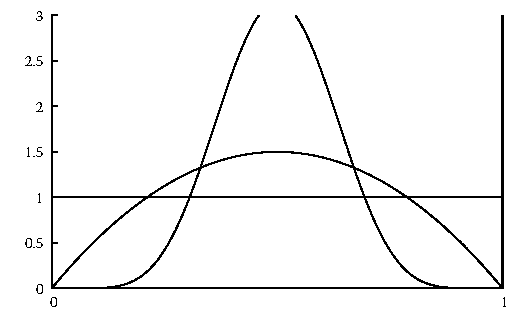
\includegraphics[width=\textwidth]{pdfBeta}
\end{center}
\caption[Beta distribution]{A beta distribution, $\opr{Beta}(0, 1, 2, 4)$}
\end{figure}

\dist{Pert} (beta-pert) distribution~\cite{Clark1962, Vose2000} is a subset of the beta distribution, parameterized by minimum ($a$), maximum ($b$) and mode ($x_\text{mode}$).  
\begin{align}
\label{Pert}
\opr{Pert}&(x\given a,b,x_\text{mode}) \checked
\\ \notag
&=  
 \frac{1}{B(\alpha, \gamma) (b-a)}
\Left(\frac{x-a}{b-a}\Right)^{\alpha-1} \Left(\frac{b-x}{b-a}\Right)^{\gamma-1} \checked
\\ \notag & \qquad x_\text{mean} = \frac{a+4x_\text{mode}+b}{6} \checked
%\\ & \qquad \alpha = 1 + 4 \frac{m-a}{b-a}, \quad \gamma = 1 + 4 \frac{b-m}{b-a}
\\ & \qquad \alpha = \frac{(x_\text{mean}-a)(2 x_\text{mode} - a - b)}{(x_\text{mode}-x_\text{mean})(b-a)} \checked
\notag 
\\\notag  & \qquad \gamma = \alpha\frac{(b-x_\text{mean})}{x_\text{mean}-a} \checked
\\ & = \opr{Beta}(x\given a,b-a,\alpha,\gamma) \checked \notag
\\ & = \opr{GenBeta}(x\given  a,b-a,\alpha,\gamma, 1)  \checked \notag
\end{align}
The PERT (Program Evaluation and Review Technique) distribution is used in project management to estimate task completion times. The {\bf modified pert} distribution replaces the estimate of the mean with $x_\text{mean}\! = \frac{a+\lambda x_\text{mode}+b}{2+\lambda}\checked$, where~$\lambda$ is an additional parameter that controls the spread of the distribution~\cite{Vose2000}.




% !TEX encoding = UTF-8 Unicode 
% !TEX root = FieldGuide.tex

\begin{table*}[tp]
\caption[Beta distribution -- Properties]{Properties of the beta distribution}
 \begin{align*}
 \text{\hyperref[PropertiesSec]{Properties}}  \quad& \\
\text{name} \quad & \op{Beta}(x\given a,s,\alpha, \gamma) 	\checked
\\
\text{PDF}\quad &    \frac{1}{B(\alpha, \gamma)}\frac{1}{ \Left|s\Right|}
\Left(\frac{x-a}{s} \Right)^{\alpha -1} \Left (1-\Left(\frac{x-a}{s}\Right)\Right)^{\gamma -1}	\checked
\hspace{-8em}
\\
\text{CDF / CCDF} \quad  & 
 \frac{B\Left( \alpha,\gamma; \sfrac{x-a}{s} \Right)}{B(\alpha,\gamma)} = I( \alpha,\gamma; \sfrac{x-a}{s})
 \checked
& {s} >0 \,\big/ \, {s} <0
\\ 
\text{parameters}\quad &   a,\ s,\ \alpha,\ \gamma, \text{ in } \Real, \\ &  \alpha,\gamma\geq0	\checked
\\
\text{support} \quad &  a \geq x \geq a+s , s>0 \quad a+s \geq x \geq a , s<0 
%\\
%\text{median} \quad   &  \cdots
\\
\text{mode} \quad  &a + s \frac{\alpha-1}{\alpha+\gamma-2}\checked  & \alpha,\gamma > 1
\\
\text{mean} \quad  &   a + s \frac{\alpha}{\alpha+\gamma}	\checked
\\
\text{variance} \quad   & s^2 \frac{\alpha\gamma}{(\alpha+\gamma)^2(\alpha+\gamma+1)} \checked
\\
\text{skew} \quad  &   \op{sgn}(s)\ \frac{2(\gamma-\alpha) \sqrt{\alpha+\gamma+1} }{(\alpha+\gamma+2)\sqrt{\alpha\gamma} } \checked
\\
\text{ex. kurtosis} \quad  &  6\frac{(\alpha-\gamma)^2(\alpha+\gamma+1) - \alpha\gamma(\alpha+\gamma+2) }{\alpha\gamma(\alpha+\gamma+2)(\alpha+\gamma+3)} \checked
\\
\text{entropy} \quad  &  \ln(|s|) + \ln\bigl(B(\alpha,\gamma)\bigr)-(\alpha-1)\psi(\alpha)
\\ &\quad {}-(\gamma-1)\psi(\gamma)+(\alpha+\gamma-2)\psi(\alpha+\gamma) \checked
\\
\text{MGF} \quad  &  \text{not simple} 
\\
\text{CF} \quad  &  {}_{1}F_{1}(\alpha; \alpha+\gamma ; i t) \checked
%\\
%E(X^h) \quad & 
\end{align*}
\end{table*}




\dist{Pearson XII} distribution~\cite{Pearson1916}: 
\begin{align}
\label{PearsonXII}
\opr{PearsonXII}(x\given a,b,\alpha) &=  \frac{1}{B(\alpha, -\alpha+2)} \frac{1}{|b-a|}\Left( \frac{x-a}{b-x} \Right)^{\alpha -1} 
\checked
\\ &= \opr{Beta}(x\given a,b-a ,\alpha, 2-\alpha) \notag  \checked
\\ &= \opr{GenBeta}(x\given a,b-a ,\alpha, 2-\alpha,1) \notag \checked
\\ \qquad 0<\alpha<2 \notag
\end{align}
A monotonic, J-shaped special case of the beta distribution noted by Pearson~\cite{Pearson1916}.

\begin{figure}[tp!]
\begin{center}
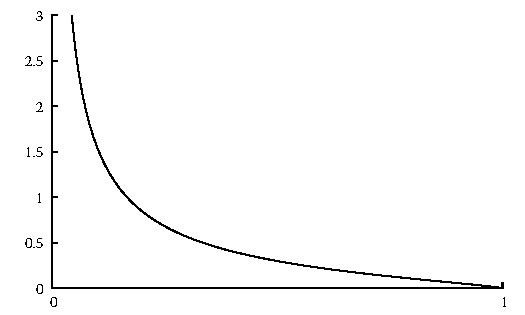
\includegraphics[width=\textwidth]{pdfPearsonXII}
\end{center}
\caption[Pearson XII distribution]{A J-shaped Pearson XII distribution, $\opr{Beta}(0, 1, \tfrac{1}{4}, 1\tfrac{3}{4})$}
\end{figure}

% ============================
\dist{Central-beta} (Pearson II, symmetric beta, generalized arcsin) distribution \cite{Pearson1895}: 
%
\begin{align}
\label{CentralBeta}
\opr{CentralBeta}(x\given \mu, b,\alpha) 
%&= \frac{1}{2s}\frac{\Gamma(2\alpha) }{ \Gamma(\alpha) } \Left(1-\frac{x^2}{4 s^2} \Right)^{\alpha-1} \\
&= \frac{1}{2^{2\alpha-1}  |b|}\frac{\Gamma(2\alpha) }{ \Gamma(\alpha)^2 } \Left(1-\Left(\frac{x-\mu}{ b}\Right)^2 \Right)^{\alpha-1}
\checked
 \\
& = \opr{Beta}(x\given \mu-b, 2b,\alpha, \alpha) 
\notag  \checked \\
& = \opr{GenBeta}(x\given \mu-b, 2 b ,\alpha, \alpha,1) \notag
\checked
\end{align}
A symmetric centered distribution with support $[\mu-b, \mu+b]$.

\begin{figure}[tp!]
\begin{center}
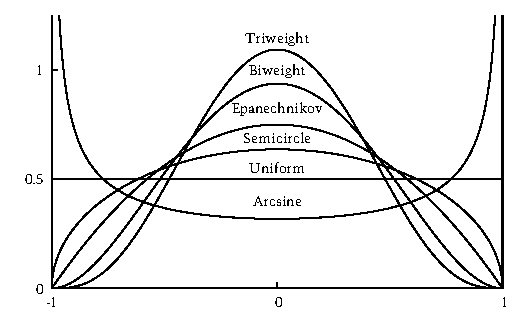
\includegraphics[width=\textwidth]{pdfPearsonII}
\end{center}
\caption[Central beta distributions]{Special cases of the central beta distribution, $\alpha=\tfrac{1}{2}, 1, \tfrac{3}{2}, 2, 3, 4$.}
\end{figure}


% ============================
\dist{Arcsine} distribution~\cite{Norton1975}:
\begin{align}
\label{Arcsine}
\opr{Arcsine}(x\given a, s) &= \frac{1}{\pi |s| \sqrt{(\tfrac{x-a}{s}) (1-\frac{x-a}{s} )}} \checked \\
& =\opr{Beta}(x\given a,s,   \tfrac{1}{2},  \tfrac{1}{2}) \notag \checked \\
& =\opr{GenBeta}(x\given a,s, \tfrac{1}{2}, \tfrac{1}{2},1) \notag \checked
\end{align}
Describes the percentage of time spent ahead of the game in a fair coin tossing contest~\cite{Johnson1995,Norton1975}. The name comes from the inverse sine function in the cumulative distribution function,
$
\op{ArcsineCDF}(x\given 0,1) = \frac{2}{\pi} \op{arcsin}( \sqrt{x}) \checked
$.



 
% ============================
\dist{Centered arcsine} distribution~\cite{Norton1975}: 
\begin{align}
\label{CenteredArcsine}
\opr{CenteredArcsine}(x\given b) &= \frac{1}{2 \pi  \sqrt{b^2-x^2}} \checked \\
%& =\opr{CentralBeta}(x\given b, \tfrac{1}{2} ) \notag \\
& =\opr{Beta}(x\given b,-2b, \tfrac{1}{2}, \tfrac{1}{2})  \checked \notag \\
& =\opr{GenBeta}(x\given b,-2b, \tfrac{1}{2}, \tfrac{1}{2},1)  \checked \notag
\end{align}
A common variant of the arcsin, with support $x\in [-b,b]$ symmetric about the origin. Describes the position at a random time of a particle engaged in simple harmonic motion with amplitude $b$~\cite{Norton1975}. With $b=1$, the limiting distribution of the proportion of time spent on the positive side of the starting position by a simple one dimensional random walk~\cite{Feller1968}.\index{diffusion}


\dist{Semicircle} (Wigner semicircle, Sato-Tate) distribution~\cite{Wigner1955}
\begin{align}
\label{Semicircle}
\opr{Semicircle}(x\given b) &= \frac{2}{\pi b^2} \sqrt{b^2-x^2} \checked \\
& =\opr{Beta}(x\given -b, 2b, 1\tfrac{1}{2}, 1\tfrac{1}{2}) \notag \checked \\
& =\opr{GenBeta}(x\given -b, 2b, 1\tfrac{1}{2}, 1\tfrac{1}{2},1) \notag \checked
\end{align}
As the name suggests, the probability density describes a semicircle, or more properly a half-ellipse. This distribution arises as the distribution of eigenvectors of various large random symmetric matrices. 

\dist{Epanechnikov} (parabolic) distribution~\cite{Epanechnikov1969a}:
\begin{align}
\label{Epanechnikov}
\opr{Epanechnikov}(x\given \mu, b) 
&= \frac{3}{4} \frac{1}{|b|} \Left(1-\Left(\frac{x-\mu}{b}\Right)^2 \Right) \checked
 \\
& = \opr{CentralBeta}(x\given \mu, b, 2) \notag \checked \\
& = \opr{Beta}(x\given \mu-b, 2 b, 2, 2) \notag   \checked \\
& = \opr{GenBeta}(x\given \mu-b, 2b, 2, 2,1) \checked \notag 
\end{align}
Used in non-parametric kernel density estimation.


\dist{Biweight} (Quartic) distribution:
\begin{align}
\label{Biweight}
\opr{Biweight}(x\given \mu, b) 
&= \frac{15}{16} \frac{1}{|b|} \Left(1-\Left(\frac{x-\mu}{b}\Right)^2 \Right)^2 
\checked
 \\
& = \opr{CentralBeta}(x\given \mu, b, 3) \notag  \checked\\
& = \opr{Beta}(x\given \mu-b, 2 b, 3, 3) \notag   \checked \\
& = \opr{GenBeta}(x\given \mu-b, 2b, 3, 3,1)  \notag \checked
\end{align}
Used in non-parametric kernel density estimation.

\dist{Triweight} distribution:
\begin{align}
\label{Triweight}
\opr{Triweight}(x\given \mu, b) 
&= \frac{35}{32} \frac{1}{|b|} \Left(1-\Left(\frac{x-\mu}{b}\Right)^2 \Right)^3 
\checked
 \\
& = \opr{CentralBeta}(x\given \mu, b, 4) \notag  \checked\\
& = \opr{Beta}(x\given \mu-b, 2 b, 4, 4) \notag   \checked \\
& = \opr{GenBeta}(x\given \mu-b, 2b, 4, 4,1)  \notag \checked
\end{align}
Used in non-parametric kernel density estimation.



\SSec{Interrelations}


The beta distribution describes the order statistics of a rectangular \eqref{Uniform} distribution.
\begin{align*}
\opr{OrderStatistic}_{\opr{Uniform}(a,s)} & (x \given \alpha, \gamma) =  \opr{Beta}(x\given a, s, \alpha, \gamma) \checked
\end{align*}
Conversely, the uniform \eqref{Uniform} distribution is a special case of the beta distribution. 
\begin{align*}
\opr{Beta}(x\given a, s, 1, 1) & = \opr{Uniform}(x\given a,s) \checked
\end{align*}


The beta and gamma distributions are related by
\[
\opr{StdBeta}(\alpha, \gamma) \sim \frac{\opr{StdGamma}_1(\alpha)} { \opr{StdGamma}_1(\alpha) + \opr{StdGamma}_2(\gamma) }
\checked
\notag
\]
which provides a convenient method of generating beta random variables, given a source of gamma random variables.


The beta distribution is a special case of the generalized beta distribution~\eqref{GenBeta}, and limits to the gamma distribution~\eqref{Gamma}.
\[
\opr{Gamma}(x\given a, \theta,\alpha)   \
& =  \lim_{\gamma\rightarrow\infty} \opr{Beta}(x\given a, \theta \gamma ,\alpha, \gamma ) \checked
\notag
\]


The Dirichlet distribution~\cite{Durbin1998,Gelman2004} is a multivariate generalization of the beta distribution. \index{Dirchlet distribution}



% !TEX encoding = UTF-8 Unicode 
% !TEX root = FieldGuide.tex

\Sec{Beta Prime Distribution}
\label{sec:BetaPrime}



\dist{Beta prime} (beta type II, Pearson type VI, inverse beta, variance ratio, gamma ratio, compound gamma,$\beta'$) distribution~\cite{Pearson1901,Johnson1995}:
\begin{align}
\label{BetaPrime}
\opr{BetaPrime}&(x\given  a, s,\alpha, \gamma) \\ \notag&= \frac{1}{B(\alpha,\gamma)}\frac{1}{|s|} \Left(\frac{x-a}{s}\Right)^{\alpha -1} \Left(1+\frac{x-a}{s}\Right)^{-\alpha-\gamma }  \checked
\\
&= \opr{GenBetaPrime}(x\given a,s, \alpha,\gamma,1) \notag \checked
\\
& \text{for }  a,\ s,\ \alpha,\ \gamma \text{ in } \Real, \  \alpha>0, \gamma>0  \checked
\notag \\ 
& \text{support } x \geq a \ \text{if}\ s > 0,  \ x\leq a  \ \text{if}\  s < 0 
\notag
\end{align}
A Pearson distribution~\secref{sec:Pearson} with semi-infinite support, and both roots on the real line. Arises notable as the ratio of gamma distributions, and as the order statistics of the uniform-prime distribution~\eqref{UniPrime}.



\SSec{Special cases}
Special cases of the beta prime distribution are listed in table~\ref{GenBetaPrimeTable}, under $\beta=1$.


\dist{Standard beta prime} (beta prime) distribution~\cite{Pearson1901}:
\begin{align}
\label{StdBetaPrime}
\opr{StdBetaPrime}(x\given \alpha, \gamma) &= \frac{1}{B(\alpha,\gamma)} x^{\alpha -1} (1+x )^{-\alpha-\gamma } \checked
\\&= \opr{BetaPrime}(x\given  0,1, \alpha,\gamma) \notag	\checked
\\&= \opr{GenBetaPrime}(x\given  0,1, \alpha,\gamma,1) \notag \checked
\end{align}


\begin{figure}[tp!]
\begin{center}
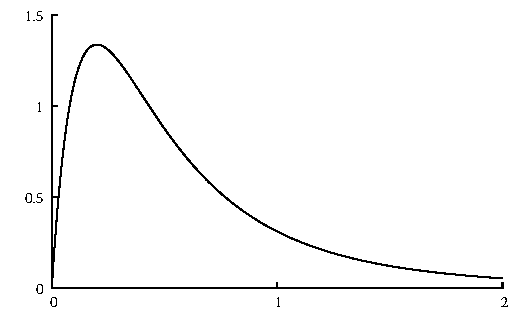
\includegraphics[width=\textwidth]{pdfBetaPrime}
\end{center}
\caption[Beta prime distribution]{A beta prime distribution, $\opr{BetaPrime}(0, 1, 2, 4)$}
\end{figure}


\dist{F} (Snedecor's F, Fisher-Snedecor, Fisher, Fisher-F, variance-ratio, F-ratio) distribution~\cite{Snedecor1934, Aroian1941, Johnson1995}:
\begin{align}
\label{F}
\opr{F}(x\given k_1,k_2) &= \frac{k_1^{\tfrac{k_1}{2} }   k_2^{\tfrac{k_2}{2}}}{ B(\tfrac{k_1}{2}, \tfrac{k_2}{2})    }
 \frac{x^{\tfrac{k_1}{2} -1}}{(k_2 + k_1 x)^{\tfrac{1}{2}(k_1+k_2)}} \checked
 \\ & =  \opr{BetaPrime}(x\given  0,\tfrac{k_2}{k_1}, \tfrac{k_1}{2},\tfrac{k_2}{2}) \notag \checked
 \\ & =  \opr{GenBetaPrime}(x\given  0,\tfrac{k_2}{k_1}, \tfrac{k_1}{2},\tfrac{k_2}{2},1) \checked
 \notag
\\ & \text{for positive integers } k_1,\ k_2 \notag \checked
\end{align}
An alternative parameterization of the beta prime distribution that derives from the ratio of two chi-squared distributions \eqref{ChiSqr} with $k_1$ and $k_2$ degrees of freedom.
\[
\opr{F}(k_1,k_2) \sim \frac{\opr{ChiSqr}(k_1) / k_1 }{\opr{ChiSqr}(k_2) / k_2} \checked
\notag
\]



\dist{Inverse Lomax} (inverse Pareto) distribution~\cite{Kleiber2003}: 
\begin{align}
\label{InvLomax}
\opr{InvLomax}(x\given a, s,\alpha) &= \frac{\alpha}{|s|} \Left(\frac{x-a}{s}\Right)^{\alpha -1} \Left(1+\frac{x-a}{s}\Right)^{-\alpha-1} \checked
\\ \notag &= \opr{BetaPrime}(x\given a, s, \alpha,1) \checked
\\ \notag &= \opr{GenBetaPrime}(x\given a, s, \alpha,1,1) \checked
\end{align}


\begin{figure}[tp!]
\begin{center}
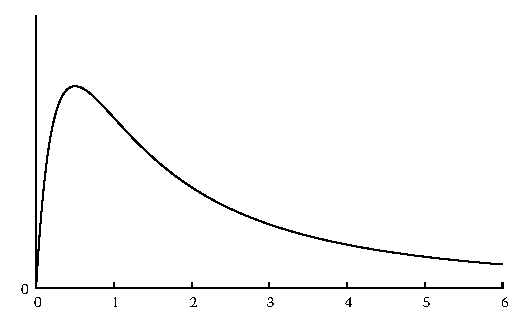
\includegraphics[width=\textwidth]{pdfInverseLomax}
\end{center}
\caption[Inverse Lomax distribution]{An inverse lomax distribution, $\opr{InvLomax}(0, 1, 2)$}
\end{figure}



% !TEX encoding = UTF-8 Unicode 
% !TEX root = FieldGuide.tex

\begin{table*}[tp]
\caption[Beta prime distribution -- Properties] {Properties of the beta prime distribution}
\begin{align*}
 \text{\hyperref[PropertiesSec]{Properties}}  \quad& \\
\text{notation} \quad & \op{BetaPrime}(x\given a, s, \alpha,\gamma)  	\checked
\\
\text{PDF}\quad &    \frac{1}{B(\alpha, \gamma)} \frac{1}{|s|}
\Left(\frac{x-a}{s}\Right)^{\alpha -1} \Left(1+ \frac{x-a}{s} \Right)^{-\alpha-\gamma } \checked
\hspace{-2em}
\\
\text{CDF / CCDF} \quad  &  
\frac{B\big(\alpha, \gamma; (1+(\tfrac{x-a}{s})^{-1})^{-1} \big) }{B(\alpha,\gamma)} \checked
\hspace{-8em}
& s >0 \,\big/ \, s<0
\\ 
& \quad = I\Left(  \alpha,\gamma; (1+(\tfrac{x-a}{s})^{-1})^{-1} \Right) 			\checked
\\
\text{parameters}\quad &   a,\ s,\ \alpha,\ \gamma, \text{ in } \Real \checked 
\\ & \alpha>0, \gamma>0 \checked
\\
\text{support} \quad &    x \geq a &  s > 0 			\checked
\\
&  x\leq a  &  s < 0 							\checked
\\
%\text{median} \quad  &  \cdots
%\\
\text{mode} \quad  & a + s \frac{\alpha-1}{\gamma+1} & \alpha\geq 1 \checked \\
& a &\alpha<1 \checked
\\
\text{mean} \quad  &   a+s \frac{ \alpha}{\gamma-1} \checked
& \gamma >1
\\
\text{variance} \quad  &s^2
\frac{\alpha(\alpha+\gamma-1)}{(\gamma-2)(\gamma-1)^2} \checked
  \hspace{-8em}
&   \gamma>2
\\
\text{skew} \quad  &  \text{not simple}
\\
\text{kurtosis} \quad  &  \text{not simple}
\\
\text{entropy} \quad  &   \ln \frac{1}{B(\alpha, \gamma)} \Left|\frac{1}{s}\Right|
  +(1-\alpha) \big[ \psi(\alpha) - \psi(\gamma)\big]
  \hspace{-8em}
\\
& \quad +(\alpha+\gamma) \big[ \psi(\alpha+\gamma) - \psi(\gamma)\big] \checked &  \text{\cite[Eq.~(15)]{Tahmasebi2010}}
\\
\text{MGF} \quad  &  \text{none}
%\\
%\text{CF} \quad  &  \cdots 
% Possible expression in terms of second confluence hypergeometric function?
% See wikipedia under F distribution
%\\
%\text{moments} \quad & \frac{B(\alpha+k,\gamma-k)}B(\alpha,\gamma)}
% Only if a =0, s=1. How do moments scale with scale?
\end{align*}
\end{table*}






\SSec{Interrelations}

The standard beta prime distribution is closed under inversion.
\[
\opr{StdBetaPrime}(\alpha,\gamma) \sim \frac{1}{\opr{StdBetaPrime}(\gamma,\alpha)} \checked
\notag
\]


The beta and beta prime distributions are related by the transformation~\secref{transforms}
\[
\opr{StdBetaPrime}(\alpha,\gamma) \sim \Left( \frac{1}{\opr{StdBeta}(\alpha,\gamma)}  -1 \Right)^{-1} \checked
\notag
\]
and, therefore, the generalized beta prime can be realized as a transformation of the standard beta \eqref{StdBeta} distribution.
\[
\opr{GenBetaPrime}(a,s,\alpha,\gamma,\beta) \sim a+ s\Left( \opr{StdBeta}(\alpha,\gamma)^{-1} -1\Right)^{-\sfrac{1}{\beta}}
\checked
\notag
\]


If the scale parameter of a gamma distribution \eqref{Gamma} is also gamma distributed, the resulting compound distribution is beta prime~\cite{Dubey1970}.
\[
\opr{BetaPrime}(0,s,\alpha,\gamma) \sim  \opr{Gamma}_2\bigl(0, \opr{Gamma}_1(0, s, \gamma),\alpha \bigr) \checked
\notag
\]
The name {\bf compound gamma distribution} is occasionally used for the anchored beta prime distribution (scale parameter, but no location parameter)

The beta prime distribution is a special case of both the generalized beta~\eqref{GenBeta} and generalized beta prime~\eqref{GenBetaPrime} distributions, and itself limits to the gamma~\eqref{Gamma} and inverse gamma~\eqref{InvGamma} distributions.
\[
\opr{Gamma}(x\given 0, \theta,\alpha)  
\notag
& =
\lim_{\gamma\rightarrow\infty} \opr{BetaPrime}(x\given 0, \theta \gamma ,\alpha, \gamma ) \checked
\\
\opr{InvGamma}(x\given \theta,\alpha) 
& =
\lim_{\gamma\rightarrow\infty} \opr{BetaPrime}(x\given 0, \theta/ \gamma ,\alpha, \gamma )  \checked
\notag
\]







% !TEX encoding = UTF-8 Unicode 
% !TEX root = FieldGuide.tex

\Sec{Beta-Exponential Distribution}
\label{sec:BetaExp}

\phantomsection
\addcontentsline{toc}{subsection}{~~~~~~~~~~~~Beta-exponential}
\phantomsection
\addcontentsline{toc}{subsection}{~~~~~~~~~~~~Standard beta-exponential}
The {\bf beta-exponential} (Gompertz-Verhulst, generalized Gompertz-Verhulst type III, 
log-beta, exponential generalized beta type I) distribution~\cite{Ahuja1967,Nadarajah2006, Iyer-Biswas2014a} is a four parameter, continuous, univariate, unimodal probability density, with  semi-infinite  support. The functional form in the most straightforward parameterization is
\begin{align}
\label{BetaExp}
\opr{BetaExp}(x\given \pLoc,\pScale,\alpha, \gamma) =&
 \frac{1}{B(\alpha, \gamma)} \frac{1}{|\pScale|}\
 e^{-\alpha \frac{x-\pLoc}{\pScale} }  \left(1 - e^{-\frac{x-\pLoc}{\pScale}  }\right)^{\gamma-1} 
 \checked
 \\ \notag
 & \text{for } x,\ \pLoc,\ \pScale,\ \alpha,\  \gamma \text{ in } \mathbb{R}, \checked
 \\ \notag & \alpha,\ \gamma >0,\quad  \tfrac{x-\pLoc}{\pScale} >0 \checked
\end{align}
The four real parameters of the beta-exponential  distribution consist of a location parameter $\pLoc$, a scale parameter $\pScale$, and two positive shape parameters $\alpha$ and $\gamma$. The {\bf standard beta-exponential} distribution has zero location $\pLoc=0$ and unit scale $\pScale=1$.


\begin{figure}[p]
\begin{center}
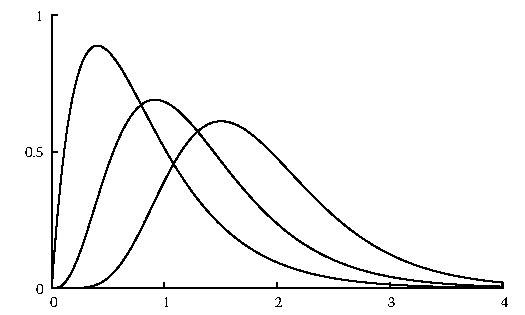
\includegraphics[width=\textwidth]{pdfBetaExp}
\end{center}
\caption[Beta-exponential distributions]{Beta-exponential distributions, (a) $\opr{BetaExp}(x\given 0,1,2, 2)$,
(b) $\opr{BetaExp}(x\given 0,1,2, 4)$,
(c) $\opr{BetaExp}(x\given 0,1,2, 8)$.
}
\end{figure}

\begin{figure}[p]
\begin{center}
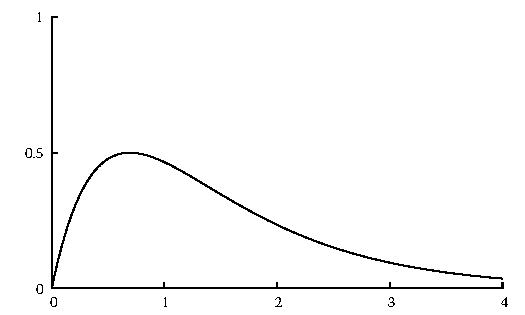
\includegraphics[width=\textwidth]{pdfExpExp}
\end{center}
\caption[Exponentiated exponential distribution]{Exponentiated exponential  distribution,  $\opr{ExpExp}(x\given 0,1,2)$.
}
\end{figure}


\begin{figure}[ht]
\begin{center}
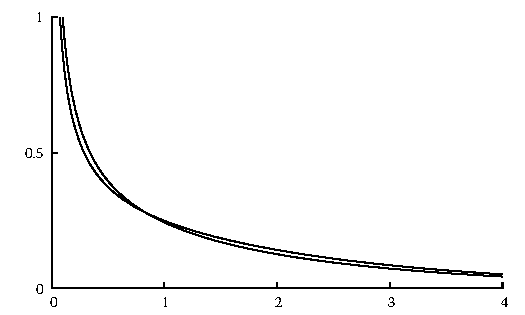
\includegraphics[width=\textwidth]{pdfSinhNK}
\end{center}
\caption[Hyperbolic sine and Nadarajah-Kotz distributions.]{Hyperbolic sine  $\opr{HyperbolicSine}(x\given \tfrac{1}{2})$ and Nadarajah-Kotz $\opr{NadarajahKotz}(x)$ distributions. }
\end{figure}



This distribution has a similar shape to the gamma \eqref{Gamma} distribution. Near the boundary the density scales like $x^{\gamma-1}$, but decays exponentially in the wing.





\SSec{Special cases}

\dist{Exponentiated exponential} (generalized exponential, Verhulst) distribution~\cite{Verhulst1847,Ahuja1967,Gupta2001}:
\begin{align}
\label{ExpExp}
\opr{ExpExp}(x\given \pLoc,\pScale,\gamma) 
 &=  \frac{\gamma}{ \left|\pScale\right|}
 e^{- \frac{x-\pLoc}{\pScale} }  \left(1 - e^{-\frac{x-\pLoc}{\pScale}  }\right)^{\gamma-1} \checked
\\ & = \opr{BetaExp}(x\given \pLoc,\pScale,1, \gamma) \notag \checked
\end{align}
A special case similar in shape to the gamma or Weibull \eqref{Weibull} distribution. So named because the cumulative distribution function is equal to the exponential distribution function raise to a power.
\[
\op{ExpExpCDF}(x\given \pLoc,\pScale,\gamma) = \big[\op{ExpCDF}(x\given \pLoc,\pScale)\big]^{\gamma}
\checked
\notag
\]
% Possibly rename Exponentiated exponential to Verhulst

\begin{table*}[bt]
%\addcontentsline{toc}{subsection}{Logistic} 
\begin{center}
\caption[Beta-exponential distribution -- Special cases]{Special cases of the beta-exponential family}
~\\
{\renewcommand{\arraystretch}{1.25} 
\begin{tabular}{llccccl}
\eqref{BetaExp} & beta-exponential & $\pLoc$ & $\pScale$ & $\alpha$ &  $\gamma$ \\
\hline  
 	& std. beta-exponential & $0$ & $1$ & . & . \\
\eqref{ExpExp} 		& exponentiated exponential & . & . & $1$ & . \\
\eqref{HyperbolicSine} & hyperbolic sine 	& . & .  & $\tfrac{1}{2}(1\text{-}\gamma)$ & $\gamma$ & $0<\gamma<1$ \\
\eqref{NadarajahKotz} &  Nadarajah-Kotz 	& . & . & $\tfrac{1}{2}$ & $\tfrac{1}{2}$ \\
%~\\
%& Related distributions \\
%\hline
\eqref{Exp} & exponential & . & . & . & $1$ \\
%\eqref{GammaExp} & gamma exponential \\ 
\end{tabular} }
\end{center}
\end{table*}


% !TEX encoding = UTF-8 Unicode 
% !TEX root = FieldGuide.tex

\begin{table*}[tp!]
\caption[Beta-exponential distribution -- Properties]{Properties of the beta-exponential distribution}
\begin{align*}
\text{\hyperref[PropertiesSec]{Properties}}  \quad& \\
\text{notation} \quad & \op{BetaExp}(x\given \pLoc,\pScale,\alpha, \gamma)  \checked
\\
\text{PDF}\quad &   \frac{1}{B(\alpha, \gamma)} \frac{1}{|\pScale|} e^{-\alpha \frac{x-\pLoc}{\pScale} }  \left(1 - e^{-\frac{x-\pLoc}{\pScale}  }\right)^{\gamma-1}  \checked
\\
\text{CDF} \big/ \text{CCDF} \quad  & I\left(\alpha,\gamma; e^{-\frac{x-\pLoc}{\pScale}} \right)\checked & \hspace{-2em}\pScale>0 \ \big/ \ \pScale<0
\\
\text{parameters}\quad &   \pLoc,\ \pScale,\ \alpha,\  \gamma \text{ in } \Real	\checked \\
& \alpha,\ \gamma >0	\checked
\\
\text{support} \quad &     x \geq \pLoc \checked&  \pScale > 0
\\
&   x\leq \pLoc  \checked&  \pScale < 0 
\\
%\text{median} \quad  &  \cdots
%\\
%\text{mode} \quad  & \text{not simple}  &\text{\cite{Nadarajah2006}}
%\\
\text{mean} \quad  &  \pLoc+ \pScale [\psi(\alpha+\gamma) -\psi(\alpha)  ]  \checked & \text{\cite{Nadarajah2006}}
\\
\text{variance} \quad  & \pScale^2 [\psi_1(\alpha)-\psi_1(\alpha+\gamma) ]  \checked & \text{\cite{Nadarajah2006}}
\\
\text{skew} \quad  &-\bigl[{\psi_2(\alpha)-\psi_2(\alpha+\gamma)}\bigr] \bigm/ {  \bigl[\psi_1(\alpha)-\psi_1(\alpha+\gamma) \bigr]^{\tfrac{3}{2}} } \checked \hspace{-2em} &  \text{\cite{Nadarajah2006}}
\\
\text{kurtosis} \quad  &
\bigl[3\psi_1(\alpha)^2- 6\psi_1(\alpha)\psi_1(\alpha+\gamma)+ 3\psi_1(\alpha+\gamma)^2+\psi_3(\alpha)
\hspace{-4em} \\ &\qquad -\psi_3(\alpha+\gamma)\bigr] \bigm/ \bigl[ \psi_1(\alpha)-\psi_1(\alpha+\gamma) \bigr]^2
\checked	
 				&  \text{\cite{Nadarajah2006}}
\\
\text{entropy} \quad  & \ln |\pScale| +\ln B(\alpha,\gamma) + (\alpha+\gamma-1) \psi(\alpha+\gamma) 
\\ & \qquad 
- (\gamma -1) \psi(\gamma) - \alpha \psi(\alpha) \checked &\text{\cite{Nadarajah2006}}
\\
\text{MGF} \quad  &e^{\pLoc t }  \frac{B(\alpha-\pScale t, \gamma) }{B(\alpha,\gamma)} \checked & \text{\cite{Nadarajah2006}}
\\                                                                                                                                              
\text{CF} \quad  & e^{i \pLoc t }   \frac{B(\alpha-i \pScale t, \gamma) }{B(\alpha,\gamma)}  \checked & \text{\cite{Nadarajah2006}}
\end{align*}
\end{table*}


\dist{Hyperbolic sine} distribution~\cite{\self}:
\begin{align}
\label{HyperbolicSine}
\opr{HyperbolicSine}(x\given \pLoc, \pScale, \gamma) 
 &=  \frac{1}{ B(\tfrac{1-\gamma}{2}, \gamma)}\frac{1}{|\pScale|}  \bigl( e^{+\frac{x-\pLoc}{2 \pScale}} - e^{-\frac{x-\pLoc}{ 2\pScale}}  \bigr)^{\gamma-1}  
 \checked
\\ \notag  &=  \frac{2^{\gamma-1}}{ B(\frac{1-\gamma}{2}, \gamma) |\pScale| } \bigl(\op{sinh}(\sfrac{x-\pLoc}{2\pScale})\bigr)^{\gamma-1} 
\checked
\\ \notag & = \opr{BetaExp}(x\given \pLoc,\pScale ,\tfrac{1-\gamma}{2}, \gamma), \quad 0<\gamma<1 
\checked
\end{align}
Compare to the hyperbolic secant distribution \eqref{HyperbolicSecant}.

\dist{Nadarajah-Kotz} distribution~\cite{Nadarajah2006,\self} : 
\begin{align}
\label{NadarajahKotz}
\opr{NadarajahKotz}(x\given \pLoc, \pScale) 
 &=  \frac{1}{\pi |\pScale|}  \frac{1}{\sqrt{e^{\frac{x-\pLoc}{\pScale}} -1}}  \checked
\\ \notag & = \opr{BetaExp}(x\given \pLoc,\pScale, \tfrac{1}{2}, \tfrac{1}{2} ) \checked
\end{align}
A notable special case when $\alpha=\gamma=\tfrac{1}{2}$. The cumulative distribution function has the simple form
\[
\op{NadarajahKotzCDF}(x\given 0, 1)= \frac{2}{\pi} \op{arctan} \sqrt{\exp(x) -1} \,  . \checked
\notag
\]
% Self citation is for name of distribution



\SSec{Interrelations}

The  beta-exponential distribution is a limit of the generalized beta distribution \secref{sec:Beta}. The analogous limit of the generalized beta prime distribution \secref{sec:BetaPrime} results in the beta-logistic family of distributions~\secref{sec:BetaLogistic}.


The beta-exponential distribution is the log transform of the beta distribution~\eqref{Beta}.
\[
\oprr{StdBetaExp}{BetaExp}(\alpha,\gamma)  \sim - \ln\bigl( \opr{StdBeta}(\alpha,\gamma) \bigr) 
\checked \notag
\]
It follows that  beta-exponential variates are related to ratios of gamma variates.
\[
\oprr{StdBetaExp}{BetaExp}(\alpha,\gamma)  \sim - \ln  \frac{\opr{StdGamma}_1(\alpha)}{\opr{StdGamma}_1(\alpha)+ \opr{StdGamma}_2(\gamma) }
\checked \notag
\]




The beta-exponential distribution describes the order statistics \secref{OrderStatistic} of the exponential distribution \eqref{Exp}.
\begin{align*}
\opr{OrderStatistic}_{\opr{Exp}(\pLoc,\pScale)} & (x \given  \gamma,\alpha) =  \opr{BetaExp}(x\given \pLoc, \pScale, \alpha, \gamma) \checked
\end{align*}
With  $\gamma=1$ we recover the exponential distribution. 
\[
\opr{BetaExp}(x\given \pLoc, \pScale, \alpha,1) = \opr{Exp}(x\given \pLoc, \tfrac{\pScale}{\alpha})
\checked \notag
\]

The beta-exponential distribution is a limit of the generalized beta distribution~\eqref{GenBeta}, and itself limits to the gamma-exponential distriution~\eqref{GammaExp}.
\[
 \notag
\opr{GammaExp}(x\given \nu, \lambda, \alpha)  & =
{\lim_{\gamma\rightarrow\infty} \opr{BetaExp}(x \given \nu+\lambda/\ln\gamma, \lambda, \alpha, \gamma)  }
\checked \notag
\]







% !TEX encoding = UTF-8 Unicode 
% !TEX root = FieldGuide.tex


\Sec{Beta-Logistic Distribution}
\label{sec:BetaLogistic} 
\phantomsection
\addcontentsline{toc}{subsection}{~~~~~~~~~~~~Beta-Logistic} 
\phantomsection
\addcontentsline{toc}{subsection}{~~~~~~~~~~~~Standard Beta-Logistic}  



The {\bf beta-logistic } (Prentice, beta prime exponential, generalized logistic type IV, exponential generalized beta prime, exponential generalized beta type II, log-F, generalized F, Fisher-Z, generalized Gompertz-Verhulst type II) distribution~\cite{Prentice1976, McDonald1991, Johnson1995, Morton2000}
 is a four parameter, continuous, univariate, unimodal probability density, with infinite  support. The functional form in the most straightforward parameterization is
\begin{align}
\notag
\label{BetaLogistic}
\opr{BetaLogistic}(x\given  \pLoc, \pScale,\alpha,\gamma) 
& =
 \frac{1}{B(\alpha, \gamma) \Left| \pScale\Right|}
 \frac{e^{-\alpha \frac{x-\pLoc}{\pScale} }} { \Left(1 + e^{-\frac{x-\pLoc}{\pScale}  }\Right)^{\alpha+\gamma} } \checked
\\  &
\ x, \pLoc, \pScale,\alpha,\gamma \text{ in } {\mathbb R}
\\ \notag & \alpha,\gamma >0
\end{align}
The four real parameters consist of a location parameter $\pLoc$, a scale parameter $\pScale$, and two positive shape parameters $\alpha$ and $\gamma$.  The {\bf standard beta-logistic} distribution has zero location $\pLoc=0$ and unit scale $\pScale=1$.

The beta-logistic distribution is perhaps most commonly referred to as `generalized logistic', but this terminology is ambiguous, since many types of generalized logistic distribution have been investigated, and this distribution is not `generalized' in the same sense used elsewhere in this survey (See `generalized' \S \ref{sec:notation}). Therefore, we select the name `beta-logistic' as a less ambiguous terminology that mirrors the names beta, beta-prime, and beta-exponential.




\SSec{Special cases}

\dist{Burr type II} (generalized logistic type I, exponential-Burr, skew-logistic) distribution~\cite{Burr1942,Johnson1994}:
\begin{align}
\label{BurrII}
\opr{BurrII}(x\given \pLoc, \pScale,  \gamma) 
& = \frac{\gamma}{|\pScale|} \frac{e^{- \frac{x-\pLoc}{\pScale} } } { \Left(1 + e^{-\frac{x-\pLoc}{\pScale}  }\Right)^{\gamma+1} }
\checked
\\
& = \opr{BetaLogistic}(x\given \pLoc, \pScale, 1, \gamma) \checked
\notag
\end{align}

\begin{figure}[t!]
\begin{center}
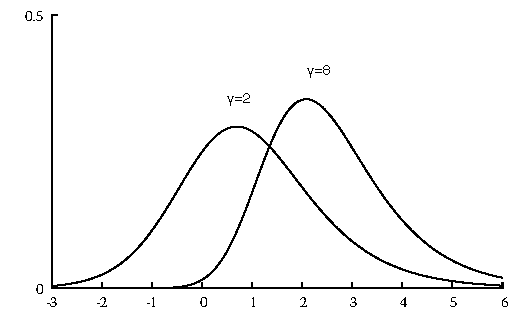
\includegraphics[width=\textwidth]{pdfBurrII}
\end{center}
\caption[Burr II distributions]{Burr type II distributions, $\opr{BurrII}(x\given0,1,\gamma)$}
\end{figure}


\dist{Reversed Burr type II} (generalized logistic type II) distribution~\cite{Johnson1994}:
\begin{align}
\label{RevBurrII}
\opr{RevBurrII}(x\given \alpha) 
& = \frac{\gamma}{|\pScale|}   \frac{e^{+ \frac{x-\pLoc}{\pScale} } } { \Left(1 + e^{+\frac{x-\pLoc}{\pScale}  }\Right)^{\gamma+1} }
\checked
\\
& = \opr{BurrII}(x\given \pLoc, -\pScale,  \gamma) \notag \checked \\
& = \opr{BetaLogistic}(x\given \pLoc, -\pScale, 1, \gamma) \notag \checked \\
& = \opr{BetaLogistic}(x\given \pLoc, +\pScale, \gamma, 1)  \notag \checked
\notag
\end{align}
By setting the $\lambda$ parameter to $1$ (instead of $\alpha$) we get a reversed Burr type II.


\begin{table*}[ptb]
%\addcontentsline{toc}{subsection}{Logistic} 
\begin{center}
\caption[Beta-logistic distribution -- Special cases]{Special cases of the beta-logistic distribution}
~\\
{\renewcommand{\arraystretch}{1.25} 
\begin{tabular}{llccccl}
\eqref{BetaLogistic} & Beta-Logistic & $\pLoc$ & $\pScale$ & $\alpha$ &  $\gamma$ \\
\hline  
\eqref{BurrII} & Burr type II					&. & . & 1 & . & \\
\eqref{RevBurrII}& Reversed Burr type II		&	. & . & . & 1 &\\
\eqref{SymBetaLogistic}& Symmetric Beta-Logistic		&	. &   . & $\alpha$ & $\alpha$ & \\
\eqref{Logistic}& Logistic					& 	. & . & 1 & 1 & \\
\eqref{HyperbolicSecant}& Hyperbolic secant	&	. & . & $\tfrac{1}{2}$ & $\tfrac{1}{2}$ & \\
\end{tabular}
}
\end{center}
\end{table*}



% !TEX encoding = UTF-8 Unicode 
% !TEX root = FieldGuide.tex

\begin{table*}[p]
\caption[Beta-logistic distribution -- Properties]{Properties of the beta-logistic distribution}
\begin{align*}
\text{\hyperref[PropertiesSec]{Properties}}  \quad& \\
\text{notation} \quad &  \op{BetaLogistic}(x\given \pLoc,\pScale,\alpha,\gamma)  
\checked
\\
\text{PDF}\quad &  
\frac{1}{B(\alpha, \gamma) \Left| \pScale\Right|}
 \frac{e^{-\alpha \frac{x-\pLoc}{\pScale} }} { \Left(1 + e^{-\frac{x-\pLoc}{\pScale}  }\Right)^{\alpha+\gamma} }
\checked 
\\
\text{CDF / CCDF} \quad  &  
 \frac{B\big(\gamma, \alpha ;  ( 1+e^{-\frac{x-\pLoc}{\pScale}} )^{-1}  \big) }{B(\alpha,\gamma)}
& \pScale>0 \, \big/ \, \pScale<0 \checked
 \text{ \cite{\self}} \\
& \qquad  = I\big(  \gamma, \alpha;  ( 1+e^{-\frac{x-\pLoc}{\pScale}} )^{-1}  \big) \checked
\\
\text{parameters}\quad &   \pLoc,\ \pScale,\ \alpha, \gamma  \text{ in } \mathbb{R} \checked \\
& \alpha,\ \gamma >0 \checked
\\
\text{support} \quad &   x \in [-\infty,+\infty] \checked
\\
%\text{median} \quad  &  \cdots
%\\
%\text{mode} \quad  & \cdots
%\\
\text{mean} \quad  &  \pLoc +\pScale [ \psi(\gamma)-\psi(\alpha) ]  \checked %\cite{McDonnald1991} Has difference in scale sign
\\
\text{variance} \quad  & \pScale^2 [\psi_1(\alpha) + \psi_1(\gamma) ] \checked %\cite{McDonnald1991}
\\
\text{skew} \quad  &  \frac{ \psi_2(\gamma) - \psi_2(\alpha)}{[\psi_1(\alpha) + \psi_1(\gamma)]^{3/2}} \checked
\\
\text{kurtosis} \quad  &   \frac{\psi_3(\alpha) + \psi_3(\gamma)}{[\psi_1(\alpha) + \psi_1(\gamma)]^{2}} \checked
\\
%\text{entropy} \quad  & \cdots
%\\
\text{MGF} \quad  &  e^{ \pLoc t}\frac{\Gamma(\alpha-\pScale  t) \Gamma(\gamma+\pScale t)}{\Gamma(\alpha)\Gamma(\gamma)}
& \text{\cite{Johnson1995}} \checked
\\
\text{CF} \quad  &    e^{i \pLoc t} \frac{\Gamma(\alpha+ i \pScale  t) \Gamma(\gamma-i \pScale t)}{\Gamma(\alpha)\Gamma(\gamma)} \checked
\end{align*}
\end{table*}




\dist{Symmetric Beta-Logistic} (generalized logistic type III, inverse cosh) distribution~\cite{Johnson1995}:
\begin{align}
\label{SymBetaLogistic}
\opr{SymBetaLogistic}(x\given \pLoc,\pScale,\alpha) 
& =
\frac{1}{B(\alpha, \alpha) |\pScale|}
 \frac{e^{-\alpha \frac{x-\pLoc}{\pScale} }} { \Left(1 + e^{-\frac{x-\pLoc}{\pScale}  }\Right)^{2\alpha} } \checked
  \\ \notag & = \frac{1}{B(\alpha, \alpha) |\pScale|} [\op{sech} \Left(\tfrac{x-\pLoc}{2\pScale}  \Right)]^{2\alpha}  
\\ \notag & = \opr{BetaLogistic}(x\given \pLoc,\pScale,\alpha,\alpha) \checked
\end{align}
With equal shape parameters the  beta-logistic is symmetric. This distribution limits to the Laplace distribution~\eqref{Laplace}.


\dist{Logistic} (sech-square, hyperbolic secant square, logit) distribution~\cite{Verhulst1845, Balakrishnan1991, Johnson1995}:
\begin{align}
\label{Logistic}
\opr{Logistic}(x\given \pLoc,\pScale) 
& =
 \frac{1}{ \Left| \pScale\Right|}
 \frac{e^{-\frac{x-\pLoc}{\pScale} }} { \Left(1 + e^{-\frac{x-\pLoc}{\pScale}  }\Right)^{2} }	\checked
 \\ \notag & = \frac{1}{4 |\pScale|} \op{sech}^2 \Left(\frac{x-\pLoc}{\pScale}  \Right)  \checked
 \\ \notag & = \opr{BetaLogistic}(x\given \pLoc,\pScale,1,1)	\checked
\end{align}





\dist{Hyperbolic secant} (Perks, inverse hyperbolic cosine, inverse cosh) distribution~\cite{Perks1932,Talacko1956, Johnson1995}:
\begin{align}
\label{HyperbolicSecant}
\opr{HyperbolicSecant}(x\given \pLoc, \pScale) 
& =
\frac{1}{\pi |\pScale|}
 \frac{1}{e^{+\sfrac{x-\pLoc}{2\pScale}} + e^{- \sfrac{x-\pLoc}{2\pScale} }} \checked
 \\ & = \frac{1}{2 \pi  |\pScale|} \op{sech}(\sfrac{x-\pLoc}{2\lambda}) \notag \checked
 \\ \notag & = \opr{BetaLogistic}(x\given  \pLoc, \pScale,\tfrac{1}{2},\tfrac{1}{2}) \checked
\end{align}
The hyperbolic secant cumulative distribution function features the Gudermannian sigmoidal function, $\op{gd}(z)$ . \index{Gudermannian function}
\begin{align*}
\op{HyperbolicSecantCDF}(x\given \pLoc, \pScale)  & = \frac{1}{\pi}\op{gd}(\frac{x-\pLoc}{2 \pScale}) \checked \\
& =  \frac{2}{\pi} \arctan(e^\frac{x-\pLoc}{2\pScale}) - \frac{1}{2} \checked
\end{align*}
The standardized hyperbolic secant distribution (zero mean, unit variance) is $\opr{HyperbolicSecant}(x\given 0, 1/\pi)\checked$.

\newcommand{\oo}{\infty}
\begin{figure}[t!]
\begin{center}
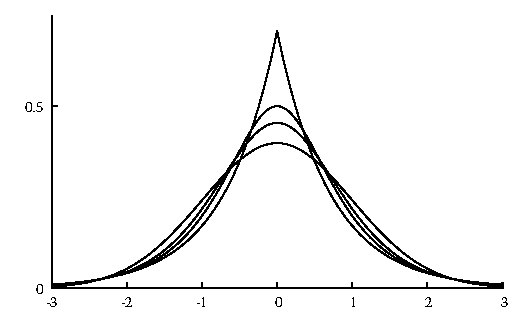
\includegraphics[width=\textwidth]{pdfSymBetaLogistic}
\end{center}
\caption[Symmetric beta-logistic distributions]{Special cases of the symmetric beta-logistic distribution~\eqref{SymBetaLogistic}: Standardized (zero mean, unit variance) normal~($\alpha\rightarrow\oo$), logistic~($\alpha=1$), hyperbolic secant~($\alpha=\tfrac{1}{2}$), and Laplace~($\alpha\rightarrow 0$)  (low to high peaks).}
\end{figure}




\SSec{Interrelations}
The beta-logistic distribution arises as a limit of the generalized beta prime distribution \secref{sec:BetaPrime}. The analogous limit of the generalized beta distribution leads to the beta-exponential family \secref{sec:BetaExp}. 


The beta-logistic distribution is the log transform of the beta prime distribution. 
\[
 \opr{BetaLogistic}(0,1,\alpha,\gamma)  \sim - \ln \opr{BetaPrime}(0,1,\alpha,\gamma)  \checked
 \notag
\] 
It follows that beta-logistic variates are related to ratios of gamma variates.
\[
\opr{BetaLogistic}(\pLoc,\pScale,\alpha,\gamma)  \sim \pLoc - \pScale \ln  \frac{\opr{StdGamma}_1(\gamma)}{\opr{StdGamma}_2(\alpha) }
\notag
\checked
\]


Negating the scale parameter is equivalent to interchanging the two shape parameters.
\[
\opr{BetaLogistic}(x\given \pLoc,+\pScale,\alpha,\gamma)  = \opr{BetaLogistic}(x\given \pLoc, - \pScale,\gamma,\alpha) \checked
\notag
\]



The beta-logistic distribution, with integer $\alpha$ and $\gamma$ is the logistic order statistics distribution~\cite{Birnbaum1963,Jones2004}~\secref{OrderStatistic}.  
\[
 \opr{OrderStatistic}_{\opr{Logistic}(\pLoc,\pScale)}  (x \given \gamma, \alpha ) =  \opr{BetaLogistic}(x\given \pLoc, \pScale, \alpha, \gamma) \checked
 \notag
\]


The beta-logistic limits to the gamma exponential~\eqref{GammaExp} and Laplace \eqref{Laplace} distributions.
\[
\opr{GammaExp}(x\given \nu, \lambda, \alpha)  & =
{\lim_{\gamma\rightarrow\infty} \opr{BetaLogistic}(x \given \nu+\lambda/\ln\gamma,\lambda, \alpha, \gamma)  }
\checked
\notag
\\
\opr{Laplace}(x\given \eta,\theta)   & = 
\lim_{\alpha\rightarrow 0} \opr{BetaLogistic}( x\given \eta, \theta\alpha\,\alpha,\alpha) \checked
\notag
\]





% !TEX encoding = UTF-8 Unicode 
% !TEX root = FieldGuide.tex

\clearpage
\Sec{Pearson IV Distribution}
%\addcontentsline{toc}{subsection}{~~~~~~~~~~~~Pearson IV} 
\label{sec:PearsonIV}

\dist{Pearson IV} (skew-$t$) distribution~\cite{Pearson1895,Heinrich2004}
is a four parameter, continuous, univariate, unimodal probability density, with infinite support. The functional form is
\begin{align}
\label{PearsonIV}
& \opr{PearsonIV}(x\given a,s, m,v) 
\\ \notag &= \frac{{}_{2}F_1(-i v, i v ; m;1)  }{|s| B(m-\frac{1}{2}, \frac{1}{2} )}  
%\times \\ \notag & \qquad 
\Left( 1 +\Left( \frac{x-a}{s}\Right)^2 \Right)^{-m}  \exp \Left\{ - 2 v \arctan \Left( \frac{x-a}{s}\Right) \Right\}
\checked
\\ \notag &=  \frac{{}_{2}F_1(-i v, i v ; m;1)  }{|s| B(m-\frac{1}{2}, \frac{1}{2} )} 
%\times \\ \notag & \qquad  
\Left( 1 + i \frac{x-a}{s} \Right)^{-m+iv} \Left( 1 -i \frac{x-a}{s} \Right)^{-m-iv}
\checked
\\ \notag & \quad x,a,s,m,v \in {\mathbb R} 
\\ \notag & \quad m>\tfrac{1}{2}
%\\ \notag & \qquad K = \frac{{}_{2}F_1(-i v, i v , m;1)  }{s B(m-\frac{1}{2}, \frac{1}{2} )} 
\end{align}
Note that the two forms are equivalent, since $\arctan(z) = \tfrac{1}{2} i \ln \frac{1-i z}{1+iz}\checked$. The first form is more conventional, but the second form displays  the essential simplicity of this distribution. The density is an analytic function with two singularities, located at conjugate points in  the complex plain, with conjugate, complex order. This is the one member of the Pearson distribution family that has not found  significant utility.


%(Note that our parameters  $a, s, m, v$ correspond to Heinrich's $\lambda, a, m, v/2$. 

\SSec{Interrelations}
The distribution parameters obey the symmetry 
\[
\opr{PearsonIV}(x\given a,s, m,v) =\opr{PearsonIV}(x\given a,-s, m,-v)\, .\checked
\notag
\] 

Setting the complex part of the exponents to zero, $v=0$, gives the Pearson VII family \eqref{PearsonVII}, which includes the Cauchy and Student's t distributions. 
\[
\opr{PearsonIV}(x\given a,s, m,0) = \opr{PearsonVII}(x\given a,s, m)  \checked
\notag
\]

Suitable rescaled,  the exponentiated arctan limits to an exponential of the reciprocal argument.
\[
 \lim_{v\rightarrow\infty} \exp(- 2 v  \arctan( -2 v x)  -  \pi  v) =  e^{-\tfrac{1}{x}}
 \checked
 \notag
\] 
% Checked with Wolfram Alpha limit_{v-> \infty} exp(- 2 v  arctan( -2 v x)  -  pi  v) 
 Consequently, the high $v$ limit of the Pearson IV distribution is an inverse gamma (Pearson V) distribution \eqref{InvGamma}, which acts an intermediate distribution between the beta prime (Pearson VI) and Pearson IV distributions.
\[
 \lim_{v\rightarrow\infty} \opr{PearsonIV}(x\given 0,-\tfrac{\theta}{2 v}, \tfrac{\alpha+1}{2},v) = \opr{InvGamma}(x\given \theta, \alpha) 
 \checked
 \notag
\]
The inverse exponential distribution \eqref{InvExp} is therefore also a special case when $\alpha=1$ ($m=1$).


%\addcontentsline{toc}{subsection}{Pearson IV} 

% !TEX encoding = UTF-8 Unicode 
% !TEX root = FieldGuide.tex

\begin{table*}[t!]
%\addcontentsline{toc}{subsection}{Pearson  IV} 
 \caption[Pearson  IV distribution -- Properties]{Properties of the Pearson  IV distribution}

\begin{align*}
\text{\hyperref[PropertiesSec]{Properties}}  \quad& \\
\text{notation} \quad & \text{PearsonIV}(x \given a,s, m,v)  
\\
\text{PDF}\quad &    \frac{{}_{2}F_1(-i v, i v ; m;1)  }{|s| B(m-\frac{1}{2}, \frac{1}{2} )} \left( 1 +\left( \frac{x-a}{s}\right)^2 \right)^{-m}
\\ \notag & \qquad \qquad \qquad \qquad \times \exp \left\{ - 2 v \arctan \left( \frac{x-a}{s}\right) \right\}
\checked
\\
\text{CDF} \quad  &    \text{PearsonIV}(x\given a,s, m,v)  \\ & \quad  \times \frac{|s|}{2m-1}\left( i - \frac{x-a}{s}\right) {}_2F_1\left(1,m+iv; 2m; \tfrac{2}{i-i\tfrac{x-a}{s}} \right) \checked
% What if s is negative? Must flip to ccdf as usual!?
% Checked against source. Good to actual check locally.
\\
\text{parameters}\quad &   a,\  s,\  m,\ v \text{ in } \Real
\\ & m>\tfrac{1}{2}
\\
\text{support} \quad &   x \in [-\infty, + \infty]
\\
%\text{median} \quad  &  \cdots
%\\
\text{mode} \quad  & a - \frac{sv}{m}  \checked
\\
\text{mean} \quad  &  a - \frac{sv}{(m-1)} \qquad (m>1) \checked
\\
\text{variance} \quad  & \frac{s^2}{2m-3} (1 + \frac{v^2}{(m-1)^2})  \qquad (m>\frac{3}{2}) \checked
\\
\text{skew} \quad  &  \text{not simple}
\\
\text{kurtosis} \quad  &  \text{not simple}
\\
\text{entropy} \quad  & \text{unknown}
\\
\text{MGF} \quad  &  \text{unknown}
\\
\text{CF} \quad  &  \text{unknown}
\end{align*}
\end{table*}








\clearpage



% Three (or more) shape parameters

% !TEX encoding = UTF-8 Unicode 
% !TEX root = FieldGuide.tex

\subpart{Three (or more) shape parameters}

\Sec{Generalized Beta Distribution}
\label{sec:GenBeta}
\phantomsection
\addcontentsline{toc}{subsection}{~~~~~~~~~~~~Generalized beta} 

The {\bf Generalized beta} (beta-power)  distribution~\cite{McDonald1984} is a five parameter,  continuous, univariate, unimodal probability density, with finite or semi infinite support. The functional form in the most straightforward parameterizaton is
\begin{align}
\label{GenBeta}
\opr{GenBeta}&(x\given a,s,\alpha, \gamma,\beta) 
\\    = & 
 \frac{1}{B(\alpha, \gamma)} \Left|\frac{\beta}{s}\Right|
\Left(\frac{x-a}{s} \Right)^{\alpha \beta -1} \Left (1-\Left(\frac{x-a}{s}\Right)^\beta\Right)^{\gamma -1}
\notag
\checked
\\
& \text{for } x,\ a,\ \theta,\ \alpha,\ \gamma,\ \beta\  \text{in } \mathbb{R}, 
\notag
\\ & \alpha>0, \  \gamma >0
\notag
 \\ \text{ support } \checked & x \in [a,a+s], s>0,\ \beta>0 \notag
  \\  &  x\in[a+s,a], s<0,\ \beta>0 
 \notag 
 \\  \notag  &  x\in[a+s,+\infty], s>0,\ \beta<0 
 \\  \notag  &  x\in[-\infty,a+s], s<0,\ \beta<0 
\notag
\end{align}
The generalized beta distribution arises as the Weibullization of the standard beta distribution, $x\rightarrow (\tfrac{x-a}{s})^{\beta}$, and as the order statistics of the power function distribution~\eqref{PowerFn}. The parameters consist of a location parameter $a$, shape parameter~$s$ and Weibull power parameter $\beta$, and two shape parameters~$\alpha$ and~$\gamma$.




\begin{table*}[tp!]
%\addcontentsline{toc}{subsection}{Beta} 
\begin{center}
\caption[Generalized beta distributions -- Special cases] {Special cases of generalized beta}
\label{GenBetaTable}
~\\

%Note: Power func special cases go under power function.
{\renewcommand{\arraystretch}{1.25} 
\begin{tabular}{llccccc@{\extracolsep{5pt}} l}
\eqref{GenBeta} &generalized beta & $a$ & $s$ & $\alpha$ & $\gamma$ & $\beta$ &
\\ \hline
\eqref{Kumaraswamy} & Kumaraswamy 		& . & . & 1 & . & . &\\
\\
\eqref{Beta} & beta				& .   & .& . & . & 1 &   \\
\eqref{StdBeta}  & standard beta 		& 0  & 1 & . & . & 1 &\\
\eqref{Beta} & beta, U shaped 		& . & . & $<\!\!1$ & $<\!\!1$ & 1 &\\
\eqref{Beta} & beta, J shaped 		& .  & . & . & . & 1 & {\small $(\alpha$-$1)(\gamma$-$1) \leq 0$} \\
\eqref{PearsonII} & Pearson II  		&  .  & . & $\alpha$ & $\alpha$ & 1 & \\
\eqref{Arcsine} & arcsine 				& .  & . & $\frac{1}{2}$ & $\frac{1}{2}$ & 1 & \\
\eqref{CentralArcsine}& central arcsine 		& -$b$  & $2b$ & $\frac{1}{2}$ & $\frac{1}{2}$ & 1 & \\
\eqref{Semicircle}& semicircle 		& -$b$  & $2b$ & $1\frac{1}{2}$ & $1\frac{1}{2}$ & 1 & \\
\eqref{Epanechnikov}&Epanechnikov & . & . & 2 & 2 & 1 \\ 
\eqref{Biweight}&Biweight & . & . & 3 & 3 & 1 \\ 
\eqref{Triweight}&Triweight & . & . & 4 & 4 & 1 \\ 
%\eqref{PowerFn} & power function		& . & . & . & 1 & 1& \\
%\eqref{PowerFn} & reciprocal		& . & . & 0 & 1 & 1& \\
%\eqref{PowerFn} & Pearson type VIII 		& 0 & . &  $<\!\!1$ & 1& 1&\\
%\eqref{PowerFn} & Pearson type IX 		& 0 & .  & $>\!\!1$ & 1 & 1&\\
\eqref{PearsonXII}  & Pearson  XII  		& . & . & . &  2-$\alpha$&1& $\alpha<2$ \\
%\eqref{Wedge} & wedge			& . & . & 2 & 1 & 1 &\\
\\
\eqref{BetaPrime} & beta prime			& . & . & . & . & -1 \\
\eqref{PowerFn} & power function		& . & . & 1 & 1 & . & \\
\eqref{Uniform} & uniform			& . & . & 1 & 1 & 1 &\\
\eqref{Uniform} & standard uniform		& 0 & 1 & 1 & 1 & 1 &\\
%\\
%& \underline{Limits}
%\\
%\eqref{UnitGamma} & unit gamma &                         . & . & $\alpha$ &.&  $\tfrac{\delta}{\alpha}$ & $\lim_{\alpha\rightarrow\infty }$ \\ 
%\eqref{Amoroso} & Amoroso			& . & $\theta \gamma^{\frac{1}{\beta}}$& . & $\gamma$ & . &    $\lim_{\gamma\rightarrow\infty}$ \\
%\eqref{BetaExp} & beta exp.			& ${\pLoc\text{-}\beta\pScale}$ & $\beta\pScale$ & . & . &$\beta$ &    $\lim_{\beta\rightarrow\infty}$ \\
\end{tabular} 
}
\end{center}
\end{table*}


% !TEX encoding = UTF-8 Unicode 
% !TEX root = FieldGuide.tex

\begin{table*}[tp]
\caption[Generalized beta distribution-- Properties]{Properties of the generalized beta distribution}
 \begin{align*}
 \text{\hyperref[PropertiesSec]{Properties}}  \quad& \\
\text{name} \quad & \text{GenBeta}(x\given a,s,\alpha, \gamma,\beta) 
\\
\text{PDF}\quad &   \frac{1}{B(\alpha, \gamma)} \left|\frac{\beta}{s}\right|
\left(\frac{x-a}{s} \right)^{\alpha \beta -1} \left(1-\left(\frac{x-a}{s}\right)^\beta\right)^{\gamma -1}
\checked
\hspace{-8em}
\\
\text{CDF / CCDF} \quad  &   \frac{B\left( \alpha,\gamma; (\tfrac{x-a}{s})^\beta  \right)}{B(\alpha,\gamma)}
\checked
% McDonald1984 table 3.1 GB1
& \tfrac{\beta}{s} >0 \,\big/ \, \tfrac{\beta}{s} <0
\\ & \quad = I\left(  \alpha,\gamma; (\tfrac{x-a}{s})^\beta \right) \checked
\\ 
\text{parameters}\quad &   a,\ s,\ \alpha,\ \gamma,\ \beta, \text{ in } \Real, \\ &  \alpha,\gamma\geq0
\\
\text{support} \quad 
&   \ x \in [a,a+s],  \quad & 0<s,\ 0<\beta  \checked
 \\ 	 		 & \ x\in[a+s,a],  \quad & s<0,\ 0<\beta   \checked
 \\  			 & \ x\in[a+s,+\infty], \quad  & 0<s,\ \beta<0  \checked
 \\  			& \ x\in[-\infty,a+s], \quad & s<0,\ \beta<0 \checked
\\
%\text{median} \quad  &  \cdots
%\\
%\text{mode} \quad  & \cdots
%\\
\text{mean} \quad  &   a+ \frac{s B(\alpha+\tfrac{1}{\beta},\gamma) }{B(\alpha,\gamma)}  \quad & \alpha+\tfrac{1}{\beta} >0
\checked
\\
\text{variance} \quad  & \frac{s^2 B(\alpha+\tfrac{2}{\beta},\gamma) }{B(\alpha,\gamma)} -\frac{s^2 B(\alpha+\tfrac{1}{\beta},\gamma)^2 }{B(\alpha,\gamma)^2} \checked
\\
\text{skew} \quad  &   \text{not simple}
\\
\text{kurtosis} \quad  &   \text{not simple}
\\
% \text{entropy} \quad  & \cdots
% \\
\text{MGF} \quad  &  \text{none} % Can't exist because beta mgf doesn't exist
\\
% \text{CF} \quad  &  \cdots
% \\
E(X^h) \quad & \frac{s^h B(\alpha+\tfrac{h}{\beta},\gamma) }{B(\alpha,\gamma)}  \qquad  & \!\!a=0,\ \alpha+\tfrac{h}{\beta} >0
\ \text{\cite{McDonald1984}} \checked
%{Normalize style, use similar style in beta properties table.}
\end{align*}
\end{table*}



\SSec{Special Cases}

The beta distribution ($\beta$=1) and specializations are described in \secref{sec:Beta}.

\dist{Kumaraswamy} (minimax) distribution~\cite{Kumaraswamy1980, Leemis2008, Jones2009}:
\begin{align}
\label{Kumaraswamy}
\opr{Kumaraswamy}(x\given a,s,\gamma,\beta) &= \gamma \Left|\frac{\beta}{s}\Right| \Left(\frac{x-a}{s}\Right)^{\beta-1} \Left(1-\Left(\frac{x-a}{s}\Right)^{\beta}\Right)^{\gamma-1} \checked
\\
&= \opr{GenBeta}(x\given a,s,1,\gamma,\beta)  \notag \checked
\end{align}
Proposed as an alternative to the beta distribution for modeling bounded variables, since the cumulative distribution function has a simple closed form, 
\[\op{KumaraswamyCDF}(x\given 0, 1, \gamma,\beta) = 1- (1-x^{\beta})^\gamma. \checked \notag\]



\SSec{Interrelations}

The generalized beta distribution describes the order statistics of a power function  distribution \eqref{PowerFn}.
\begin{align*}
\opr{OrderStatistic}_{\opr{PowerFn}(a,s,\beta)} &(x \given \alpha, \gamma) = \opr{GenBeta}(x\given a, s, \alpha,\gamma, \beta) 
\checked
\end{align*}
Conversely, the power function \eqref{PowerFn} distribution is a special case of the generalized beta distribution. 
\begin{align*}
\opr{GenBeta}(x\given a, s, 1, 1,\beta) & = \opr{PowerFn}(x\given a,s,\beta)  \checked
\notag
\end{align*}

Setting $\beta=1$ yields the beta  distribution \eqref{Beta}, 
\[
\opr{GenBeta}(x\given a,s,\alpha, \gamma,1) = \opr{Beta}(x\given a,s,\alpha,\gamma) \ , \checked
\notag
\]
and setting $\beta=-1$ yields the beta prime (or inverse beta) distribution \eqref{BetaPrime},  
\[
\opr{GenBeta}(x\given a,s,\alpha, \gamma,-1) = \opr{BetaPrime}(x\given a+s,s,\gamma,\alpha) \ . \checked
\notag
\]
The beta \secref{sec:Beta} and beta prime \secref{sec:BetaPrime} distributions have many named special cases, see tables~\ref{GenBetaTable} and \ref{GenBetaPrimeTable}.


The unit gamma distribution~\eqref{UnitGamma} arises in the limit $\lim_{\beta\rightarrow0}$ with $\alpha\beta=\text{constant}$,
\[
 \lim_{\beta\rightarrow0 } \opr{GenBeta}(x\given a,s,\tfrac{\delta}{\beta}, \gamma,\beta)  = \opr{UnitGamma}(x\given a, s, \gamma,\delta) \ . \checked
 \notag
\]
In the  limit $\gamma\rightarrow\infty$ (or equivalently $\alpha\rightarrow\infty$) we obtain the Amoroso distribution \eqref{Amoroso} with semi-infinite support, the parent of the gamma distribution family~\cite{McDonald1984},
\[
\lim_{\gamma\rightarrow\infty} \opr{GenBeta}(x\given a, \theta \gamma^{\frac{1}{\beta}} ,\alpha, \gamma, \beta ) = \opr{Amoroso}(x\given a,\theta,\alpha, \beta) \ . \checked
\notag
\]
The limit  $\lim_{\beta\rightarrow+\infty }$ yields the beta-exponential distribution~\eqref{BetaExp}
\[
 \lim_{\beta\rightarrow+\infty } \opr{GenBeta}(x\given \pLoc+\beta\lambda,-\beta\pScale,\alpha,\gamma,\beta) = \opr{BetaExp}(x\given \pLoc,\pScale,\alpha, \gamma) \checked
\ .
\notag
\]






% !TEX encoding = UTF-8 Unicode 
% !TEX root = FieldGuide.tex

\Sec[Gen. Beta Prime Distribution] {Generalized Beta Prime Distribution}
\label{sec:GenBetaPrime}
\phantomsection
\addcontentsline{toc}{subsection}{~~~~~~~~~~~~Generalized beta prime} 
The {\bf Generalized beta prime} (Feller-Pareto, beta-log-logistic, generalized\linebreak gamma ratio, Majumder-Chakravart, generalized beta type II, generalized Feller-Pareto)  distribution~\cite{Feller1971, McDonald1984, Tahmasebi2010} is a five parameter,  continuous, univariate, unimodal probability density, with semi-infinite support. The functional form in the most straightforward parameterization is
\begin{align}
\label{GenBetaPrime}
\opr{GenBetaPrime}&(x\given a, s, \alpha,\gamma,\beta) \\
& =
 \frac{1}{B(\alpha, \gamma)} \Left|\frac{\beta}{s}\Right|
\Left(\frac{x-a}{s}\Right)^{\alpha\beta -1} \Left(1+ \Left(\frac{x-a}{s}\Right)^\beta \Right)^{-\alpha-\gamma }
\notag
\checked
\\ & \quad a,\ s,\ \alpha,\ \gamma,\ \beta \text{ in } \mathbb{R},\quad  \alpha,\ \gamma >0
\notag
\end{align}
The five real parameters of the generalized beta prime distribution consist of a location parameter~$a$, 
scale parameter~$s$, two shape parameters,~$\alpha$ and~$\gamma$, and the Weibull power parameter $\beta$. The shape parameters, $\alpha$ and $\gamma$, are positive.


The generalized beta prime arises as the Weibull transform of the standard beta prime distribution \eqref{StdBetaPrime}, and as order statistics of the log-logistic distribution. The Amoroso distribution is a limiting form, and a variety of other distributions occur as special cases. (See Table~\ref{GenBetaPrimeTable}).  These distributions are most often encountered as parametric models for survival statistics developed by  economists and actuaries.




\SSec{Special cases}



\dist {Transformed beta} distribution~\cite{McDonald1984,Klugman2012}:
\begin{align}
\label{TransformedBeta}
\opr{TransformedBeta}&(x\given s, \alpha,\gamma,\beta) 
\\ \notag & =
 \frac{1}{B(\alpha, \gamma)} \Left|\frac{\beta}{s}\Right|
\Left(\frac{x}{s}\Right)^{\alpha\beta -1} \Left(1+ \Left(\frac{x}{s}\Right)^\beta \Right)^{-\alpha-\gamma }
\checked
\\ \notag &= \opr{GenBetaPrime}(x\given 0, s, \alpha,\gamma,\beta) 
\checked
\end{align}
A generalized beta prime distribution without a location parameter, $a=0$.


\dist{Burr}  (Burr type XII, Pareto type IV, beta-P, Singh-Maddala, generalized log-logistic, exponential-gamma,Weibull-gamma) 
%q-exponential\sscite{Nadarajah2006}) %This dosn't compute.
distribution~\cite{Burr1942,Tadikamalla1980, Kleiber2003}:
\begin{align}
\label{Burr}
\opr{Burr}(x\given a, s, \gamma,\beta) 
&=  
 \frac{\beta \gamma}{|s|} \Left(\frac{x-a}{s}\Right)^{\beta-1}  \Left(1+\Left(\frac{x-a}{s}\Right)^\beta\Right)^{-\gamma-1} 
 \checked
\\ & = \opr{GenBetaPrime}(x\given a, s, 1,\gamma,\beta) \notag   \checked
\end{align}
Most commonly encountered as a model of income distribution.



\begin{table*}[tp]
%\addcontentsline{toc}{subsection}{Beta prime} 
\begin{center}
\caption[Generalized beta prime distribution -- Special cases]{Special cases of generalized beta prime}
\label{GenBetaPrimeTable}
~\\
{\renewcommand{\arraystretch}{1.25} 
\begin{tabular}{llccccc}
\eqref{GenBetaPrime}  & generalized beta prime & $a$ & $s$ & $\alpha$  &  $\gamma$ & ${\beta}$  \\
\hline
\eqref{Burr} & Burr 	        			&  .  &  .  &  1  &  .    &    .     \\
\eqref{Dagum} & Dagum			&  0  &  1 &  .  &  1   &    .     \\
\eqref{Paralogistic} & paralogistic			&  0 &  1  &  1  &  $\beta$    &    .     \\
\eqref{InvParalogistic} & inverse paralogistic	&  0 &  1  &   $\beta$& 1    &    .     \\
\eqref{LogLogistic} & log-logistic			&  0  &  . &  1  &  1  &    .     \\
\eqref{GenBetaPrime} & transformed beta			&  0  &  . &  .  &  .  &    .     \\
\eqref{HalfGenPearsonVII} & half gen. Pearson VII 		&  .  &  . &  $\tfrac{1}{\beta}$  &  $m$-$\tfrac{1}{\beta}$  &    .     \\
\eqref{BetaPrime} & beta prime		& . & . & . & . & 1  \\
\eqref{Lomax} & Lomax 				&  .  &  . &  1  &  .   &    1     \\
\eqref{InvLomax} & inverse Lomax 				&  .  &  . &  .  &  1   &    1     \\
\eqref{StdBetaPrime} & std. beta prime		& 0 & 1 & . & . & 1  \\
\eqref{F} & F	&  0 &  $\tfrac{k_2}{k_1}$ & $\tfrac{k_1}{2}$ & $\tfrac{k_2}{2}$   &    1     \\
\eqref{UniPrime} & uniform-prime	& . & . & 1 & 1 & 1  \\
\eqref{ExpRatio} & exponential ratio		& 0 & . & 1 & 1 & 1  \\
\eqref{HalfPearsonVII} & half-Pearson  VII	&  . &  .  &   $\tfrac{1}{2}$ & .   &    2     \\
\eqref{HalfCauchy} & half-Cauchy	&  . &  . & $\tfrac{1}{2}$ & $\tfrac{1}{2}$   &    2     \\
\end{tabular} 
}
\end{center}
\end{table*}


% !TEX encoding = UTF-8 Unicode 
% !TEX root = FieldGuide.tex

\begin{table*}[p]
\caption[Generalized beta prime distribution -- Properties]{Properties of the generalized beta prime distribution}
\begin{align*}
 \text{\hyperref[PropertiesSec]{Properties}}  \quad& \\
\text{notation} \quad & \text{GenBetaPrime}(x\given a, s, \alpha,\gamma,\beta)   \checked
\\
\text{PDF}\quad &    \frac{1}{B(\alpha, \gamma)} \Left|\frac{\beta}{s}\Right|	
\Left(\frac{x-a}{s}\Right)^{\alpha\beta -1} \Left(1+ \Left(\frac{x-a}{s}\Right)^\beta \Right)^{-\alpha-\gamma } \checked
\hspace{-30em}
\\
\text{CDF / CCDF} \quad  &  
\frac{B\big(\alpha, \gamma; (1+(\tfrac{x-a}{s})^{-\beta})^{-1} \big) }{B(\alpha,\gamma)} \checked
\hspace{-7em}
& \tfrac{\beta}{s} >0 \,\big/ \, \tfrac{\beta}{s} <0
\\ 
& \quad = I\Left(  \alpha,\gamma; (1+(\tfrac{x-a}{s})^{-\beta})^{-1} \Right)  \checked
% See McDonald1984, table 3.1 GB2. Expresses incomplete beta function as hypergeometric function.
\\
\text{parameters}\quad &   a,\ s,\ \alpha,\ \gamma,\ \beta \text{ in } \Real \checked 
\\ & \alpha>0, \gamma>0	\checked
\\
\text{support} \quad &    x \geq a &  s > 0 										
\\
&  x\leq a  &  s < 0 
\\
%\text{median} \quad  &  \cdots
%\\
% \text{mode} \quad  & \cdots
% \\
\text{mean} \quad  &   a+\frac{s B(\alpha+\tfrac{1}{\beta},\gamma- \tfrac{1}{\beta}) }{B(\alpha,\gamma)} 
\checked &   -\alpha< \tfrac{1}{\beta} <\gamma \checked
% % See McDonald1984, table 3.1 GB2
\\
\text{variance} \quad  &s^2\Left[\frac{ B(\alpha+\tfrac{2}{\beta},\gamma- \tfrac{2}{\beta}) }{B(\alpha,\gamma)} -  \Left(\frac{ B(\alpha+\tfrac{1}{\beta},\gamma- \tfrac{1}{\beta}) }{B(\alpha,\gamma)}\Right)^2 \Right]  \hspace{-15em}
& -\alpha< \tfrac{2}{\beta} <\gamma \checked
\\
\text{skew} \quad  &  \text{not simple}
\\
\text{kurtosis} \quad  &  \text{not simple}
%\\
%\text{entropy} \quad  &   \ln \frac{1}{B(\alpha, \gamma)} \Left|\frac{\beta}{s}\Right|
%  +(\tfrac{1}{\beta}-\alpha) \big[ \psi(\alpha) - \psi(\gamma)\big]
%  \hspace{-7em} 
%  \\
%& \quad +(\alpha+\gamma) \big[ \psi(\alpha+\gamma) - \psi(\gamma)\big] \checked & \text{\cite[Eq.~(15)]{Tahmasebi2010}} % Not correct?
\\
% \text{MGF} \quad  &  \cdots
% \\
% \text{CF} \quad  &  \cdots
% \\
E[ X^h]  \quad & \frac{|s|^h B(\alpha+\tfrac{h}{\beta},\gamma- \tfrac{h}{\beta}) }{B(\alpha,\gamma)} 
& \!\!a=0,\  -\alpha< \tfrac{h}{\beta} <\gamma \quad   \text{\cite{McDonald1984}} \checked
\end{align*}
\end{table*}






\dist{Dagum} (Inverse Burr, Burr type III, Dagum type I,  beta-kappa, beta-k, Mielke) distribution~\cite{Burr1942, Dagum1977, Tadikamalla1980}:
\begin{align}
\label{Dagum}
\opr{Dagum}(x\given  \gamma,\beta) 
%&= \gamma \beta \frac{x^{\gamma\beta-1}}{ (1+x^\beta)^{\gamma +1} }  \\
&=  \frac{\beta \gamma}{|s|} \Left(\frac{x-a}{s}\Right)^{\gamma \beta-1}  \Left(1+\Left(\frac{x-a}{s}\Right)^\beta\Right)^{-\gamma-1} 
\checked
%\\ \notag &= \opr{Burr}(x\given a,s,  \gamma,-\beta) \checked % Burr restricted to positive beta
\\ \notag &= \opr{GenBetaPrime}(x\given a, s, 1, \gamma,-\beta) \checked
\\ \notag &= \opr{GenBetaPrime}(x\given a, s, \gamma,1,+\beta) \checked
\end{align}

\dist{Paralogistic} distribution~\cite{Kleiber2003}:
\begin{align}
\label{Paralogistic}
\opr{Paralogistic}(x\given a, s, \beta) &= \frac{\beta^2}{|s|} \frac{ \Left(\frac{x-a}{s}\Right)^{\beta-1}}{ (1+ \Left(\frac{x-a}{s}\Right)^\beta)^{\beta+1} } \checked
\\ \notag &= \opr{GenBetaPrime}(x\given a, s, 1,\beta,\beta)
\checked
\end{align}


\dist{Inverse paralogistic} distribution~\cite{Klugman2012}:
\begin{align}
\label{InvParalogistic}
\opr{InvParalogistic}(x\given a,s,\beta) &= \frac{\beta^2}{|s|}  \frac{ \Left(\frac{x-a}{s}\Right)^{\beta^2-1}}{ (1+ \Left(\frac{x-a}{s}\Right)^\beta)^{\beta+1} } \checked
\\ \notag &= \opr{GenBetaPrime}(x\given a, s, \beta,1,\beta) \checked
\end{align}





\dist{Log-logistic} (Fisk, Weibull-exponential, Pareto type III, power prime) distribution~\cite{Shah1963, Johnson1995}:
\begin{align}
\label{LogLogistic}
\opr{LogLogistic}(x\given a,s,\beta) &=\Left|\frac{\beta}{s}\Right| \frac{\Left(\frac{x-a}{s}\Right)^{\beta-1}}{ \Left(1+\Left(\frac{x-a}{s}\Right)^{\beta}\Right)^{2} } \checked
\\ \notag &= \opr{Burr}(x\given a, s, 1,\beta) \checked
\\ \notag &= \opr{GenBetaPrime}(x\given 0, s, 1,1,\beta) \checked
\end{align}
Used as a parametric model for survival analysis and, in economics, as a model for the distribution of wealth or income.
The logistic and log-logistic distributions are related by an exponential transform. 
\[
\opr{LogLogistic}(0,s,\beta) &\sim  \exp\bigl(-\opr{Logistic}(-\ln s,\sfrac{1}{\beta})\bigr) 
\checked
\notag
\]

\begin{figure}[t]
\begin{center}
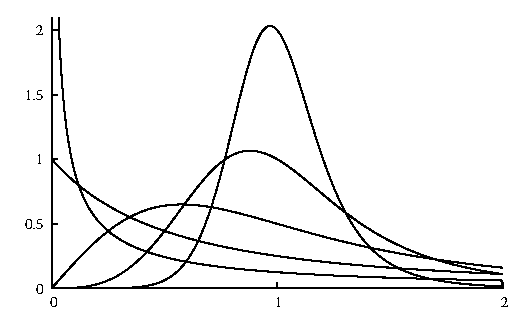
\includegraphics[width=\textwidth]{pdfLogLogistic}
\end{center}
\caption[Log-logistic distributions]{Log-logistic distributions, $\opr{LogLogistic}(x\given 0,1,\beta)$.}
\end{figure}




\dist{Half-Pearson VII} (half-t) distribution~\cite{Gelman2006}: 
\begin{align}
\label{HalfPearsonVII}
 \opr{HalfPearsonVII}&(x\given a, s, m)  \\
\notag &=
 \frac{1}{B(\tfrac{1}{2},m-\tfrac{1}{2})} \frac{2}{|s|}
 \Left(1+ \Left(\frac{x-a}{s}\Right)^2 \Right)^{-m} \checked
\\ \notag & =  \opr{GenBetaPrime}(x\given a, s, \tfrac{1}{2},m-\tfrac{1}{2}, 2) \checked
\end{align}
The Pearson type VII \eqref{PearsonVII} distribution truncated at the center of symmetry. Investigated as a prior for variance parameters in hierarchal models~\cite{Gelman2006}.



\dist{Half-Cauchy} distribution~\cite{Gelman2006}: 
\begin{align}
\label{HalfCauchy}
\opr{HalfCauchy}(x\given a, s)  &=
 \frac{2}{\pi |s|}
 \Left(1+ \Left(\frac{x-a}{s}\Right)^2 \Right)^{-1}
 \checked
 \\ \notag & =  \opr{HalfPearsonVII}(x\given a, s, 1) \checked
\\ \notag & =  \opr{GenBetaPrime}(x\given a, s, \tfrac{1}{2},\tfrac{1}{2}, 2)  
\checked
\end{align} 
A notable subclass of the Half-Pearson type VII, the Cauchy distribution \eqref{Cauchy} truncated at the center of symmetry.


\dist{Half generalized Pearson VII} distribution~\cite{\self}: 
\begin{align}
\label{HalfGenPearsonVII}
\opr{HalfGenPearsonVII}&(x\given a,s, m,\beta)  
\\ \notag = & \frac{\beta}{ |s| B(m-\frac{1}{\beta}, \frac{1}{\beta} )} \Left( 1 +\Left( \frac{x-a}{s}\Right)^{\beta} \Right)^{-m} 
\checked
\\ \notag & =  \opr{GenBetaPrime}(x\given a, s, \tfrac{1}{\beta},m-\tfrac{1}{\beta}, \beta) 
\checked
%\\ \notag & x, a,s, m,\beta \text{ in } {\mathbb R} \\
%&  \tfrac{x-a}{s}>0,\  \beta>0,\ m>0,\ \beta m >1
%\notag
\end{align}
One half of a Generalized Pearson VII distribution~\eqref{GenPearsonVII}. 
Special cases include half Pearson VII \eqref{HalfPearsonVII}, half Cauchy \eqref{HalfCauchy}, {\bf half Laha} (See \eqref{Laha}),  and uniform prime \eqref{UniPrime} distributions. 
\begin{align*}
\opr{HalfGenPearsonVII}(x\given a,s, m,2) &= \opr{HalfPearsonVII}(x\given a,s,m) \checked \\
\opr{HalfGenPearsonVII}(x\given a,s, 1,2) &= \opr{HalfCauchy}(x\given a,s) \checked \\
\opr{HalfGenPearsonVII}(x\given a,s, 1,4) &= \oprr{HalfLaha}{Laha}(x\given a,s) \checked \\
\opr{HalfGenPearsonVII}(x\given a,s, 2,1) &= \opr{UniPrime}(x\given a,s)  \checked 
\end{align*}
The half exponential power \eqref{HalfExpPower} distribution occurs in the large $m$ limit.
\begin{align*}
\lim_{m\rightarrow\infty} \opr{HalfGenPearsonVII}&(x\given a,\theta m^{\sfrac{1}{\beta}}, m,\beta) 
 = \opr{HalfExpPower}(x\given a,\theta,\beta) \checked
\end{align*}
\phantomsection
\addcontentsline{toc}{subsection}{~~~~~~~~~~~~Half Laha}



% ====================================================================
\SSec{Interrelations}


Negating the Weibull parameter of the generalized beta prime distribution is equivalent to exchanging the shape parameters  $\alpha$ and $\gamma$.
\begin{align*}
\opr{GenBetaPrime}&(x\given a, s, \alpha,\gamma,\beta)  = \opr{GenBetaPrime}(x\given a, s,\gamma, \alpha,-\beta) \checked
\end{align*}

The distribution is related to ratios of gamma distributions.
\[
\opr{GenBetaPrime}(a,s,\alpha,\gamma,\beta) \sim a+ s\Left( \frac{\opr{StdGamma}_1(\alpha)}{\opr{StdGamma}_2(\gamma) } \Right)^{\tfrac{1}{\beta}} \checked
\notag
\]

Limit of the generalized beta prime distribution include the Amoroso \eqref{Amoroso}~\cite{McDonald1984} and beta-logistic \eqref{BetaLogistic} distributions.
\begin{align*}
\lim_{\gamma\rightarrow\infty} \opr{GenBetaPrime}(x\given a, \theta \gamma^{\frac{1}{\beta}} ,\alpha, \gamma, \beta )  
%\\ 
& = \opr{Amoroso}(x\given a,\theta,\alpha, \beta) \checked \\
\lim_{\beta\rightarrow\infty}  \opr{GenBetaPrime}(x\given  \pLoc+\beta\pScale, -\beta \pScale, \alpha, \gamma, \beta)  
 %\\
 & = \opr{BetaLogistic}(x\given \pLoc,\pScale, \gamma, \alpha) \checked
\end{align*}
Therefore, the generalized beta prime also indirectly limits to the normal \eqref{Normal}, log-normal \eqref{LogNormal}, gamma-exponential \eqref{GammaExp}, Laplace \eqref{Laplace} and power-function \eqref{PowerFn} distributions, among others.

Generalized beta prime describes the order statistics \secref{OrderStatistic} of the log-logistic distribution \eqref{LogLogistic}). 
\begin{align*}
 \opr{OrderStatistic}_{\opr{LogLogistic}(a,s,\beta)}(x \given \gamma, \alpha ) & =  \opr{GenBetaPrime}(x\given a, s, \alpha, \gamma, \beta)  \checked
\end{align*}


Despite occasional claims to the contrary,
the log-Cauchy distribution is not a special case of the generalized beta prime distribution (generalized beta prime is mono-modal, log-Cauchy is not).





% =================================================================================


% !TEX encoding = UTF-8 Unicode 
% !TEX root = FieldGuide.tex

\Sec{Pearson Distribution}
\label{sec:Pearson}
\phantomsection
\addcontentsline{toc}{subsection}{~~~~~~~~~~~~Pearson} 
The {\bf Pearson} distributions~\cite{Pearson1895, Pearson1901, Pearson1916, Ord1972, Johnson1994} are a family of continuous, univariate, unimodal probability densities with distribution function
\begin{align}
\label{Pearson}
 \opr{Pearson}&(x\given a, s\sep a_1, a_2\sep  b_0, b_1, b_2) 
 \\ \notag
 &=  \tfrac{1}{\mathcal{N}} \Left(1- \tfrac{1}{r_0}\tfrac{x-a}{s} \Right)^{e_0} \Left(1- \tfrac{1}{r_1}\tfrac{x-a}{s} \Right)^{e_1}
\\ \notag
&  a,\ s,\  a_1,\ a_2,\ b_0,\ b_1,\ b_2,\ x\  \text{ in } \mathbb{R}
\\ \notag
& r_0 = \tfrac{-b_1+\sqrt{b_1^2 - 4b_2b_0} }{2b_2} \checked  \qquad e_0 = \tfrac{-a_1-a_2 r_0}{r_1-r_0} \\
\notag
& r_1 = \tfrac{-b_1-\sqrt{b_1^2 - 4b_2b_0} }{2b_2} \checked \qquad e_1 = \tfrac{a_1+a_2 r_1}{r_1-r_0} 
\end{align}
Here $\mathcal{N}$ is the normalization constant. Note that the parameter $a_2$  is redundant, and can be absorbed into the scale. Thus the Pearson distribution effectively has 4 shape parameters. We retain $a_2$ in the general definition since this makes parameterization of subtypes easier. 


Pearson constructed his family of distributions by requiring that they satisfy the differential equation
\begin{align*}
\frac{d}{dx} \ln  \opr{Pearson}(x\given 0, 1\sep a_1, a_2\sep b_0, b_1, b_2) 
&= - \frac{a_1 + a_2 x  }{b_0+ b_1 x+ b_2 x^2  } \ ,  \checked \\
&= - \frac{1}{x} \frac{\phantom{a_0 + {} } a_1 x + a_2 x^2  }{b_0+ b_1 x+ b_2 x^2  } \ ,  \checked \\
&= \frac{e_0}{x-r_0} + \frac{e_1}{x-r_1} \ . \checked
\end{align*}
Pearson's original motivation was that the discrete hypergeometric distribution obeys an analogous finite difference relation~\cite{Ord1972}, and that at the time very few continuous, univariate, unimodal probability distributions had been described. The numbering of the $a_1, a_2$ coefficients is chosen to be consistent with Weibull transformed generalization of the Pearson distribution \eqref{GUD}, where an $a_0$ parameter naturally arises. 


The Pearson distribution has three main subtypes determined by~$r_0$ and~$r_1$, the roots of the quadratic denominator. First, we can have two roots located on the real line, at the minimum and maximum of the distribution. This is commonly known as the beta distribution \eqref{Beta}. (The parameterization is based on standard conventions.)
\[
p(x) \propto x^{\alpha-1} (1-x)^{\gamma-1}, \qquad 0<x<1 \checked
\notag
\]
The second possibility is that the distribution has semi infinite support, with one root at the boundary, and the other located outside the distribution's support. This is the beta prime distribution.  \eqref{BetaPrime} (Again, the parameterization is based on standard conventions.)
\[
p(x) \propto x^{\alpha-1} (1+x)^{-\alpha-\gamma}, \qquad 0<x<+\infty
\notag
\checked
\]
The third possibility is that the distribution has an infinite support with both roots located off the real axis in the complex plane.  To ensure that the distribution remains real, the roots must be complex conjugates of one another. In this case, the root order can also be complex conjugates of one another. This is Pearson's type IV distribution \eqref{PearsonIV}. (The complex roots and powers can be disguised with trigonometric functions and some algebra, at the cost of making the distribution look more complex than it actually is.)
\[
p(x) \propto (i-x)^{m+iv} (i+x)^{m-iv}, \qquad -\infty <x<+ \infty \checked
\notag
\]
The Cauchy distribution, for instance, is a special case of Pearson's type IV distribution.




\SSec{Special cases}

A large number of useful distributions are members of Pearson's family (See Fig.~\ref{PearsonHierarchy}). Pearson identified 13 principal subtypes -- the normal distribution and types I through XII (See table~\ref{PearsonTypesTable}). 
In Fig.~\ref{PearsonHierarchy} and table~\ref{PearsonTable2} we consider 12 principal subtypes. (We include the uniform, inverse exponential and Cauchy as distributions important in their own right, and give less prominence to Pearson's types VIII, IX, XI and XII.)
All of the Pearson distributions have great utility and are widely applied, with the exception of Pearson IV (infinite support, complex roots with complex powers) \eqref{PearsonIV}, which appears rarely (if at all) in practical applications. 

\dist{q-Gaussian} (symmetric Pearson) distribution~\cite{Leeuwen1995} :
\begin{align}
\label{QGaussian}
\opr{QGaussian}(x\given \mu,\sigma,q) &= \frac{1}{\sqrt{2\sigma^2}  \ \mathcal{N}} \exp_q\Left(-\half \Left(\tfrac{x-\mu}{\sigma}\Right)^2 \Right) \checked
\\
 \notag
& = \frac{1}{\sqrt{2\sigma^2} \ \mathcal{N}}  \Left(1- \half (1-q) \Left(\tfrac{x-\mu}{\sigma}\Right)^2 \Right)^{\frac{1}{1-q} } \checked
\\
& -2 < q < 3
\notag
\\
x \in (-\infty, +\infty) &\text{ for } 1\leq q < 3
\notag
\\
x \in (\mu-{\tfrac{\sqrt{2}\sigma}{\sqrt{1-q}}}, \mu+{\tfrac{\sqrt{2}\sigma}{\sqrt{1-q}}}) & \text{ for } q < 1
\notag
\end{align}
Here $ \exp_q$ is the q-generalized exponential function \secref{sec:math}. The normalization constant is
\begin{align*}
\mathcal{N} &=
 \begin{cases} 
 \sqrt{\pi} \frac{   {2  \Gamma\Left({\frac{1}{1-q}}\Right)} }{ {(3-q) \sqrt{1-q} \Gamma\Left(\frac{3-q }{ 2(1-q)} \Right)}  } 
 & -2 <q < +1 \checked
\\
  \sqrt{\pi} & \phantom{-2<}q=+1  \checked
\\
 \sqrt{\pi}  \frac{{\Gamma\Left({\frac{3-q}{2(q-1)}}\Right)} }{ {\sqrt{q-1} \Gamma\Left(\frac{1 }{ q-1}\Right)}}&  +1<q<+3 \checked
\end{cases}
 \end{align*}

A special case of the Pearson family that interpolates between all of the symmetric Pearson distributions: the central beta \eqref{CentralBeta}, normal \eqref{Normal} and Pearson VII \eqref{PearsonVII} families. See also the hierarchy of symmetric distributions in Fig.~\ref{SymmetricHierarchy}.
\begin{align*}
\opr{QGaussian}&(x\given \mu,\sigma,q) \\ &=
%\\
 \begin{cases}
\opr{Beta}(x\given a-\tfrac{\sqrt{2}\sigma}{\sqrt{1-q}},\tfrac{2\sqrt{2}\sigma}{\sqrt{1-q}},\tfrac{2-q}{1-q},\tfrac{2-q}{1-q}) 
 & -2 <q < 1 \checked
 \\
\opr{CentralBeta}(x\given a,\tfrac{\sqrt{2}\sigma}{\sqrt{1-q}}, \tfrac{2-q}{1-q}) 
 & -2 <q < 1 \checked
\\
\opr{Normal}(x\given \mu,\sigma)   & \phantom{1<}q=1  \checked
\\
 \opr{PearsonVII}(x\given a,\tfrac{\sqrt{2}\sigma}{\sqrt{q-1}}, \tfrac{1}{q-1}) &  1<q<3 \checked
\end{cases}
 \end{align*}



\begin{table}
\begin{center}
\caption{Pearson's categorization}
\label{PearsonTypesTable}
\begin{tabular}{clll}
\\
type & notes & Eq. & Ref.\\
\hline
 & normal & \eqref{Normal} & \cite{Pearson1895}  \\
I  & beta & \eqref{Beta} & \cite{Pearson1895}  \\
II &  central-beta & \eqref{CentralBeta} & \cite{Pearson1895}  \\
III  &   gamma & \eqref{Gamma}& \cite{Pearson1893}  \\
IV  & Includes Pearson VII & \eqref{PearsonIV}& \cite{Pearson1895}  \\
V   &  inverse gamma & \eqref{InvGamma}& \cite{Pearson1901}  \\
VI   & beta prime &  \eqref{BetaPrime} & \cite{Pearson1901}  \\
VII   & Includes Cauchy and Student's t  &\eqref{PearsonVII} & \cite{Pearson1916}  \\ 
VIII   & Special case of power function & \eqref{PowerFn} & \cite{Pearson1916}  \\
IX  & Special case of power function & \eqref{PowerFn} & \cite{Pearson1916}  \\
X   & exponential & \eqref{Exp} & \cite{Pearson1916}  \\
XI   & Pareto & \eqref{Pareto} & \cite{Pearson1916}  \\
XII   & J-shaped beta  &\eqref{PearsonXII} & \cite{Pearson1916}  \\
\end{tabular}
\end{center}
\end{table}




\begin{table*}[tb]
\begin{center}
\caption[Pearson distribution -- Special cases]{Special cases of the Pearson distribution}
\label{PearsonTable2}
{\renewcommand{\arraystretch}{1.25} 
\begin{tabular}{llccccrrr}
\\
\eqref{Pearson}  & Pearson & $a$ & $s$ & $a_1$ & $a_2$  & $b_0$ & $b_1$ & $b_2$ \\
\hline
\eqref{Uniform} 	& uniform 		&  $a$  &  $s$  &  $0$  &  $0$    &     $0$    & $1$ & $-1$  \checked\\
\eqref{CentralBeta} 	& central-beta 	&  $\mu$-$b$  &  $2b$  &  $\alpha-1$  &  $2\alpha-2$    &    $0$   & $1$ &$-1$ \checked\\
\eqref{Beta}     		& {beta} 		&  $a$  &  $s$  &  $\alpha-1$  &  $\alpha+\gamma-2$  &  $0$    &    $1$    &  $-1$  \checked \\
\eqref{Exp} 		& exponential 	&  $a$  &  $\theta$  &  $0$  &  $-1$    &    $0$    & $1$ & $0$ \checked \\
\eqref{Gamma} 	& gamma 		&  $a$  &  $\theta$  &  $\alpha-1$  &  $-1$    &    $0$    & $1$ & $0$ \checked \\
\eqref{BetaPrime} 	& {beta-prime} 	&  $a$  &  $s$  &  $\alpha-1$  &  $-\gamma-1$  &  $0$    &    $1$    &  $1$\\
\eqref{InvGamma} 	& inv.~gamma 	&  $a$  &  $\theta$  &  $-1$  &  $\alpha+1$  &      $0$    & $0$ & $1$ \checked \\
\eqref{InvExp} 		& inv.~exp.&$a$ &  $\theta$  &  $-1$  &  $2$    &     $0$    & $0$ & $1$ \checked \\
\eqref{PearsonIV} 	& {Pearson IV} 	&  $a$  &  $s$  &  $2v$  &  $2m$  &  $1$    &    $0$    & $1$\\
\eqref{PearsonVII} 	& Pearson VII 	&  $a$  &  $s$  &  0  &  $2m$  &  $1$    &    $0$    & $1$ \checked\\
\eqref{Cauchy} 	& Cauchy 		&  $a$  &  $s$  &  0  &  $2$  &    $1$    &    $0$    & $1$  \checked \\
\eqref{Normal} 		& normal 		&$\mu$&  $\sigma$  &  $0$  &  $2$    &    $1$    &    $0$    & $0$ \\
\end{tabular} 
}
\end{center}
% Uniform could actual be any b's?
% Gamma	D[Log[x^{a-1} Exp[-x] ], x]
% Beta 		D[Log[x^{a-1} (1-x)^{g-1} ], x]
% Inv Gamma  D[Log[ x^(-a-1) Exp[-x^{-1}]],x]
% Inv Exp		D[Log[ x^(-2) Exp[-x^{-1}]], x]
\end{table*}



% !TEX encoding = UTF-8 Unicode 
% !TEX root = FieldGuide.tex

\Sec{Grand Unified Distribution}
\label{sec:GUD}



The Grand Unified Distribution of order $n$ is required to satisfy the following differential equation.
\begin{align}
\label{GUD}
\frac{d}{dx} \ln  \opr{GUD}^{(n)}&(x\given a, s \sep a_0, a_1,\ldots,a_n\sep  b_0,b_1,\ldots, b_n\sep \beta)
\checked \\
&= -\Left|\tfrac{\beta}{s}\Right| \frac{1}{\bigl(\tfrac{x-a}{s}\bigr)} \frac{a_0  +a_1 \bigl(\tfrac{x-a}{s}\bigr)^{\beta}+\cdots +a_n \bigl(\tfrac{x-a}{s}\bigr)^{n\beta}}{b_0+ b_1 \bigl(\tfrac{x-a}{s}\bigr)^{\beta}+\cdots+b_n\bigl(\tfrac{x-a}{s}\bigr)^{n\beta}  } 
\notag
\checked
\\
& \qquad  a,\ s,\  a_0,a_1,\ldots,a_n,\ b_0,b_1, \ldots, b_n,\ \beta,\ x\  \text{ in } \mathbb{R} 
\checked
\notag
\\ \notag
& \qquad \beta = 1 \text{ when } a_0 =0
\checked
\end{align}
In principal, any analytic probability distribution can satisfy this relation.
The central hypothesis of this compendium is that most interesting univariate continuous probability distributions satisfy this relation with low order polynomials in the denominator and numeration. If fact, there seems be little need to consider beyond $n=2$, which we take as the default order, in the absence of further qualification. 



\SSec{Special cases}

\dist{Extended Pearson} distribution~\cite{Roy1971}: With $\beta=1$ we obtain an extended Pearson distribution.
\begin{align}
\label{ExtPearson}
&\frac{d}{dx} \ln  \opr{ExtPearson}(x\given 0, 1\sep a_0, a_1, a_2\sep b_0, b_1, b_2) \checked \\
\notag
&= - \frac{1}{x} \frac{a_0 +a_1 x+ a_2 x^2}{b_0+ b_1 x+  b_2 x^2  } \\
\notag
& a,\ s,\ a_0,\ a_1,\ a_2,\ b_0,\ b_1,\ b_2 \text{ in } \Real
\end{align}



\begin{figure*}
\thispagestyle{chapter}
\caption[Grand Unified Distributions]{Grand Unified Distributions} 
\begin{center}
\scalebox{0.6} {
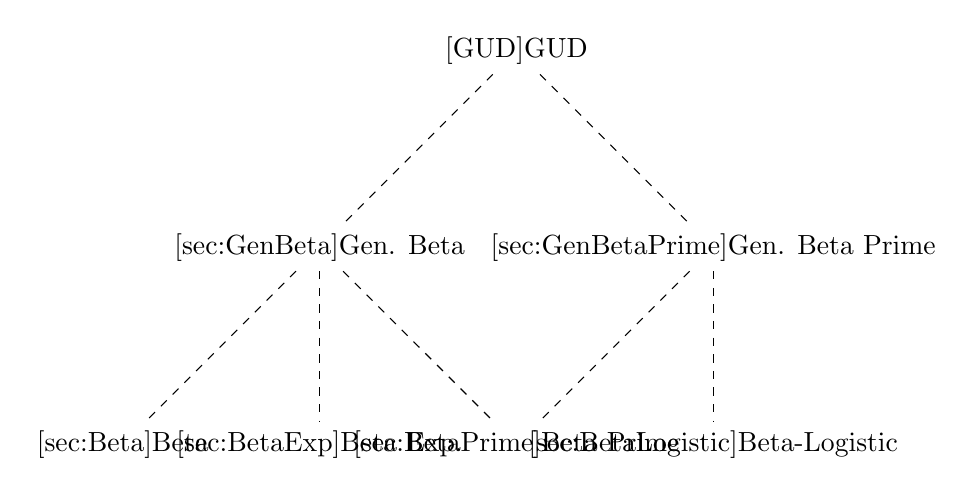
\begin{tikzpicture}
%\draw[help lines, very thin, step=1] (-2,0) grid (17,17);
%
%\draw (7.5,16.75) node (ExtPearson) {\hyperref[ExtPearson]{Ext. Pearson}};
%%\draw (7.5,15) node (PearsonExp) {\hyperref[PearsonExp]{Pearson Exp.}};
%\draw (7.5,16.75) node (ExtPearson) {\hyperref[ExtPearson]{Ext. Pearson}};

\draw (7.5,17.5) node (gud) {\hyperref[GUD]{GUD}};
%
\draw (5,15) node (genbeta) {\hyperref[sec:GenBeta]{Gen. Beta}};
%\draw (7.5,15) node (pearson) {\hyperref[sec:Pearson]{Pearson}};
\draw (10,15) node (genbetaprime) {\hyperref[sec:GenBetaPrime]{Gen. Beta Prime}};
%
\draw (2.5,12.5) node (beta) {\hyperref[sec:Beta]{Beta}};
\draw (5,12.5) node (betaexp) {\hyperref[sec:BetaExp]{Beta Exp.}};
\draw (7.5,12.5) node (betaprime) {\hyperref[sec:BetaPrime]{Beta Prime}};
\draw (10,12.5) node (betalogistic) {\hyperref[sec:BetaLogistic]{Beta-Logistic}};
%\draw (12.5,12.5) node (pearsoniv) {\hyperref[sec:PearsonIV]{Pearson IV}};
%
%\draw (2.5,10) node (unitgamma) {\hyperref[sec:UnitGamma]{Unit Gamma}};
%\draw (7.5,10) node (amoroso) {\hyperref[sec:Amoroso]{Amoroso}};
%\draw (12.5,10) node (burr) {\hyperref[Burr]{Burr}};
%
\draw [dashed]  (gud) -- (genbeta);
%\draw [dashed]  (gud) -- (pearson);
\draw [dashed]  (gud) -- (genbetaprime);
%%\draw [dashed]  (gud) -- (PearsonExp);
%%\draw [dashed]  (PearsonExp) -- (betaexp);
%%\draw [dashed]  (PearsonExp) -- (betalogistic);
%
\draw [dashed]  (genbeta) -- (beta);
\draw [dashed]  (genbeta) -- (betaexp);
\draw [dashed]  (genbeta) -- (betaprime);
%\draw [dashed]  (genbeta) -- (unitgamma);
%\draw [dashed]  (genbeta) -- (amoroso);
%
%\draw [dashed]  (pearson) -- (beta);
%\draw [dashed]  (pearson) -- (betaprime);
%\draw [dashed]  (pearson) -- (pearsoniv);
%
\draw [dashed]  (genbetaprime) -- (betalogistic);
\draw [dashed]  (genbetaprime) -- (betaprime);
%\draw [dashed]  (genbetaprime) -- (amoroso);
%\draw [dashed]  (genbetaprime) -- (burr);
%
%\draw[|-|, very thin] (-1.5,0.5) -- node[fill=white, midway] {0} (-1.5,3);
%\draw[|-|, very thin]  (-1.5,4.5) -- node[fill=white, midway] {1} (-1.5,8);
%\draw[|-|, very thin]  (-1.5,9.5) -- node[fill=white, midway] {2} (-1.5,13);
%\draw[|-|, very thin]  (-1.5,14.5) -- node[fill=white, midway] {3} (-1.5,15.5);
%\draw[|-|, very thin]  (-1.5,16) -- node[fill=white, midway] {4} (-1.5,17);
%
%
%\draw (-1, 15.75) node[rotate=90]  {\small shape parameters};
%
%\draw[white] (-2, 0) rectangle (17,17.5); % Bounding box
\end{tikzpicture}
}
\end{center}
\end{figure*}




\begin{table*}[bp]
\begin{center}
\caption[Grand Unified Distribution -- Special cases]{Special cases of the Grand Unified Distribution}
{\renewcommand{\arraystretch}{1.25} 
\begin{tabular}{llcccccccccc}
\eqref{GUD}  & GUD & $a$ & $s$ & $a_0$ & $a_1$ & $a_2$ & $b_0$ & $b_1$ & $b_2$  & $\beta$ \\
\hline
\eqref{ExtPearson} & Ext.\ Pearson  &.&.&.&.&.&.&.&.&$1$ \checked\\
\eqref{Pearson}	 & Pearson  &.&.&0&.&.&.&.&.&$1$ \checked\\
\eqref{GenBeta} & gen.\ beta &.&.&.&.&0&0&1&-1&. \checked\\
\eqref{GenBeta} & gen.\ beta prime &.&.&.&.&0&0&1&1&. \checked\\
\eqref{InvGaussian}	 & inv.\ Gaussian &.&.&.&$\tfrac{3}{2}$&.&0&1&0&1 \checked \\
\eqref{RecInvGaussian}   & rec.\ inv.\ Gaussian$\!\!\!\!$ &.&.&.&$\tfrac{3}{2}$&.&0&1&0&-1 \\
\eqref{Halphen} & Halphen &.&.&$-\kappa$&$1$-$\alpha$&$\kappa$&0&1&0&1 \checked \\
\eqref{GenHalphen} & gen.\ Halphen &.&.&$-\kappa$&$1$-$\alpha$&$\kappa$&0&1&0&$\beta$ \\
\eqref{Hyperbola} & Hyperbola &.&.&$-\kappa$&1&$\kappa$&0&1&0&1 \checked \\
\eqref{HalphenB} & Halphen B&.&.&$1$-$\alpha$&$-\kappa$&$2$&0&1&0&1 \checked \\
\eqref{InvHalphenB} & inv.\ Halphen B&.&.&$1$-$\alpha$&$-\kappa$&$-2$&0&1&0&1 \checked \\
\eqref{Sichel} & Sichel &.&.&$-\lambda$&$1$-$\alpha$&$\kappa$&0&1&0&1 \checked \\
\eqref{GenSichel} & gen.\ Sichel &.&.&$-\lambda$&$1$-$\alpha$&$\kappa$&0&1&0&$\beta$ \\
\end{tabular} 
}
\end{center}
\end{table*}


%===========================================================================
\dist{Inverse Gaussian} (Wald, inverse normal) distribution~\cite{Wald1944,Tweedie1945,Folks1978,Chhikara1989,Johnson1994}: 
\begin{align}
\label{InvGaussian}
\opr{InvGaussian}(x\given \mu,\lambda) &= \sqrt{\frac{\lambda}{2\pi x^3}} \exp\Left(\frac{-\lambda (x-\mu)^2}{2\mu^2 x}\Right) \checked
\\ \notag
& = \opr{ExtPearson}(x\given 0,1 \sep -\tfrac{\lambda}{2}, \tfrac{3}{2}, \tfrac{\lambda}{2\mu^2} \sep 0, 1,0) \checked
\\ \notag
& = \opr{GUD}(x\given 0,1 \sep -\tfrac{\lambda}{2}, \tfrac{3}{2}, \tfrac{\lambda}{2\mu^2} \sep  0, 1,0 \sep 1) \checked
\end{align}
with support $x>0$, mean $\mu>0$, and shape $\lambda>0$. The name `inverse Gaussian' is misleading, since this is not in any direct sense the inverse of a Gaussian distribution. 
The {\bf Wald} distribution is a special case with $\mu=1$.
% D[-Log[sqrt(L /(2 pi x^3)) exp(-{L(x- m)^2} / {2m^2 x})], x]

The inverse Gaussian distribution describes first passage time in one dimensional Brownian diffusion with drift~\cite{Chhikara1989}. The displacement $x$ of a diffusing particle after a time $t$, with diffusion constant $D$ and drift velocity $v$,  is $\opr{Normal}(vt, \sqrt{2 D t})$. The `inverse' problem is to ask for the first passage time, the time taken to first reach a particular position $y>0$, which is distributed as $\opr{InvGaussian}(\tfrac{y}{v},\tfrac{y^2}{2D})$. \index{first passage time}\index{diffusion}

In the limit that $\mu$ goes to infinity we recover the L\'evy distribution \eqref{Levy}, the first passage time distribution for Brownian diffusion without drift.
\[
\lim_{\mu\rightarrow\infty} \opr{InvGaussian}(x\given \mu, \lambda) = \Levy(x\given 0,\lambda) \checked
\notag
\]

The sum of independent inverse Gaussian random variables is also inverse Gaussian, provided that $\mu^2/\lambda$ is a constant.
\begin{align*}
\sum_i \opr{InvGaussian}_i &(x\given \mu' w_i, \lambda' w_i^2) 
\\
& \sim \opr{InvGaussian}\Bigl(x\given \mu' \sum_i w_i, \lambda' \bigl(\sum_i w_i\bigr)^2 \Bigr) \checked
\end{align*}

Scaling an inverse Gaussian scales both $\mu$ and $\lambda$. 
\[
c\ \opr{InvGaussian} (\mu, \lambda) \sim \opr{InvGaussian} (c \mu, c \lambda) \checked
\notag
\]

It follows from the previous two relations the sample mean of an inverse Gaussian is inverse Gaussian.
\[
\frac{1}{N} \sum_{i=1}^N \opr{InvGaussian}_i (\mu, \lambda) \sim \opr{InvGaussian} (\mu, N \lambda) \checked
\notag 
\]



\dist{Reciprocal inverse Gaussian} distribution~\cite{Johnson1994}: 
\begin{align}
\label{RecInvGaussian}
\opr{RecInvGaussian}(x\given \mu,\lambda) &= \sqrt{\frac{\lambda}{2\pi x}} \exp\Left(\frac{-\lambda (1-\mu x)^2}{2\mu^2 x}\Right) \checked
\\ \notag
& = \opr{ExtPearson}(x\given 0,1 \sep -\tfrac{\lambda}{2\mu^2}, \tfrac{1}{2}, \tfrac{\lambda}{2} \sep 0, 1,0) \checked
\\ \notag
& = \opr{GUD}(x\given 0,1 \sep -\tfrac{\lambda}{2}, \tfrac{3}{2}, \tfrac{\lambda}{2\mu^2} \sep 0, 1,0 \sep -1) \checked
\end{align}
with support $x>0$, mean $\mu>0$, and shape $\lambda>0$. An inverted (in standard sense) inverse Gaussian distribution. 
\[
\opr{RecInvGaussian}(\mu,\lambda) \sim \opr{InvGaussian}(\mu,\lambda)^{-1}
\notag
\]
% D[-Log[sqrt(L /(2 pi x)) exp(-{L(1- m x)^2} / {2m^2 x})], x]



\dist{Halphen} (Halphen A) distribution~\cite{Halphen1941}:
\begin{align}
\label{Halphen}
&\opr{Halphen}(x\given a,s, \alpha, \kappa) 
\\
&= \frac{1}{2 |s| K_{\alpha} (2\kappa)} \Left(\frac{x-a}{s}\Right)^{\alpha-1} 
\exp\Left\{-\kappa \Left(\frac{x-a}{s}\Right) -\kappa \Left(\frac{x-a}{s}\Right)^{-1}\Right\},
\checked
\notag
\\
 &=  \op{GUD}(x\given a,s \sep -\kappa, 1-\alpha, \kappa\sep 0,1,0 \sep 1)
\notag
\checked
\\& \qquad  0 \leq \tfrac{x-a}{s}
\notag
\end{align}
Developed by \'Etienne Halphen for the frequency analysis of river flows.
Limits to gamma, inverse gamma, and normal.



% D[log(x^{(-1)} e^{-k x -k/x}),x]
% D[log(x^{(a-1)} e^{-k x -k/x}),x]
% D[log(x^{(a-1)} e^{-x^2 +k x}),x]
% D[log(x^{(a-1)} e^{-x^(-2) +k / x}),x]
% Sichel: D[log(x^{(a-1)} e^{-k x -L/x}),x]
\dist{Hyperbola} (harmonic) distribution~\cite{Halphen1941,Perreault1999}:
\begin{align}
\label{Hyperbola}
&\opr{Hyperbola}(x\given a,s,\kappa) 
\\ 
&= \frac{1}{2 |s| K_0(2\kappa)} \Left(\frac{x-a}{s}\Right)^{-1} 
\exp \Left\{ -\kappa \Left(\frac{x-a}{s}\Right) -\kappa \Left(\frac{x-a}{s}\Right)^{-1} \Right\},
\checked
\notag
\\
& = \op{Halphen}(x\given a,s, 0, \kappa) 
\checked
\notag
\\
& = \op{GUD}(x\given a,s\sep -\kappa, 1 , \kappa\sep 0,1,0\sep 1) 
\checked
\notag
\\& \qquad  0 \leq \tfrac{x-a}{s}
\notag
\end{align}




\dist{Halphen B} distribution~\cite{Halphen1941,Perreault1999}:
\begin{align}
\label{HalphenB}
&\opr{HalphenB}(x\given a,s, \alpha, \kappa) 
\\
&= \frac{2}{|s| H_{2 \alpha}(\kappa)} \Left(\frac{x-a}{s}\Right)^{\alpha-1} 
\exp\Left\{- \Left(\frac{x-a}{s}\Right)^{2} +\kappa \Left(\frac{x-a}{s}\Right)\Right\},
\checked
\notag
\\
& = \op{GUD}(x\given a,s\sep 1-\alpha, -\kappa,  2\sep 1,0,0\sep 1) \checked
\notag
\\& \qquad  0 \leq \tfrac{x-a}{s}
\notag
\end{align}
The normalizing function $H_{2 \alpha}(\kappa)$ was called the exponential factorial function by Halphen~\cite{Halphen1955a, Perreault1999}.
Limits to gamma distribution \eqref{Gamma} as $\kappa \rightarrow \infty$.
\index{exponential factorial function}

% According to Perreault1999, cite Morlat1956a not Halphen1941
\dist{Inverse Halphen B} distribution~\cite{Morlat1956a,Perreault1999}:
\begin{align}
\label{InvHalphenB}
&\opr{InvHalphenB}(x\given a,s, \alpha, \kappa) 
\\
&= \frac{2}{|s| H_{2\alpha}(\kappa)} \Left(\frac{x-a}{s}\Right)^{-\alpha+1} 
\exp\Left\{- \Left(\frac{x-a}{s}\Right)^{-2} +\kappa \Left(\frac{x-a}{s}\Right)^{-1}\Right\},
\checked
\notag
\\
& = \op{GUD}(x ; a,s; 1-\alpha, \kappa,  -2; 0,0,1;1) \checked
\notag
\\& \qquad  0 \leq \tfrac{x-a}{s}
\notag
\end{align}
Limits to inverse gamma distribution \eqref{InvGamma} as $\kappa \rightarrow \infty$.

\dist{Sichel} (generalized inverse Gaussian) distribution~\cite{Good1953, Sichel1973, Barndorff-Nielsen1977}:
\begin{align}
\label{Sichel}
&\opr{Sichel}(x\given a,s, \alpha, \kappa, \lambda) 
\\
&= \frac{(\kappa/\lambda)^{\alpha/2} }{2 |s| K_{\alpha} (2\sqrt{\kappa\lambda})} \Left(\frac{x-a}{s}\Right)^{\alpha-1} 
\exp\Left\{-\kappa \Left(\frac{x-a}{s}\Right) -\lambda \Left(\frac{x-a}{s}\Right)^{-1}\Right\},
\notag
\checked
\\
& = \op{GUD}(x \given a,s \sep -\lambda, 1-\alpha , \kappa \sep 0,1,0 \sep 1)
\notag
\\& \qquad  0 \leq \tfrac{x-a}{s} \notag
\end{align}
Special cases include Halphen \eqref{Halphen} $\lambda= \kappa$, and inverse Gaussian \eqref{InvGaussian} $\alpha = -\tfrac{1}{2}$.




\dist{Libby-Novick} distribution~\cite{Libby1982a, McDonald1995, Sarabia2006, Nadarajah2007}
\begin{align}
\label{LibbyNovick}
&\opr{LibbyNovick}(x\given a,s,c,\alpha,\gamma) 
\\ \notag
&=  \frac{1}{|s| B(\alpha,\gamma)}
\Left(\tfrac{x-a}{s}\Right)^{\alpha-1}  \Left(1-\tfrac{x-a}{s}\Right)^{\gamma-1} \Left(1- (1-c) \tfrac{x-a}{s}\Right)^{-\alpha-\gamma}
\checked
\notag
\\ \notag
& = \op{GUD}(x|a,s; \alpha-1, 3-\alpha - c - c\gamma, 2c-2; 
\\ \notag & \qquad\qquad\qquad 1, c-2, 1-c;1) \checked
\\ \notag
& \qquad \text{for } a,s,c,\alpha,\gamma  \text{ in } {R},  \alpha,\gamma  >0
\\ \notag
& \qquad 0\leq \tfrac{x-a}{s} \leq1
\end{align}
A generalized three-parameter beta distribution that arises naturally as a beta distribution style ratio of gamma distributions~\cite{Sarabia2006}. 
\[
\opr{LibbyNovick}(0, \tfrac{s_1}{s_2}, \alpha, \gamma) \sim \frac{\opr{Gamma}_1(0, s_1,\alpha)} { \opr{Gamma}_1(0, s_1,\alpha) + \opr{Gamma}_2(0, s_2,\gamma) }
\notag
\checked
\]
Limits to both the beta ($u=1$) and beta-prime ($u\rightarrow \infty$ ) distributions. 
% D[Log[x^(a-1)(1-x)^(g-1)(1-(1-u)x)^(-a-g)], x]

\dist{Gauss hypergeometric} distribution~\cite{Armero1994,Sarabia2006}
\begin{align}
\label{GaussHypergeometric}
&\opr{GaussHypergeometric}(x\given a,s,u, \alpha, \gamma, \delta) 
\\ \notag
& =   \frac{1}{|s| \mathcal{N}} 
\Left(\frac{x-a}{s}\Right)^{\alpha-1}  \Left(1-\frac{x-a}{s}\Right)^{\gamma-1} \Left(1- (1-u) \frac{x-a}{s}\Right)^{-\delta}
\checked
\notag
\\ \notag
& \quad \mathcal{N} = B(\alpha,\gamma)\  {}_2F_1(\alpha,\delta;\alpha+\gamma,1-u)  \checked
\\ \notag
& \qquad \text{for } a, s, u,\alpha,\gamma, \delta  \text{ in } \mathbb{R},  \alpha,\gamma, \delta >0
\\ \notag &
=\op{GUD}(x\given a, s \sep \alpha-1,2 - \alpha -\gamma + (1-u)(1+ \rho+\alpha), \checked \\
& \qquad\qquad \qquad\notag
u(\alpha+\gamma-\rho-2) \sep 1, -1-c, -u \sep 1)
\\ \notag
& \qquad 0\leq \tfrac{x-a}{s} \leq1
\end{align}
A natural generalization of the three-beta distribution.  Motivated by the Euler integral formula for the Gauss hypergeometric function~\secref{sec:math}. 


\dist{Confluent hypergeometric} distribution~\cite{Gordy1988a,Nadarajah2006a,Nadarajah2007}
\begin{align}
\label{Confluent}
\opr{Confluent}&(x \given \alpha, \gamma, \delta) 
\\& =
\notag
\frac{1}{\mathcal{N}}  
\Left(\frac{x-a}{s}\Right)^{\alpha-1} \Left(1- \Left(\frac{x-a}{s}\Right)\Right)^{\gamma-1} \exp\Left\{-\kappa \Left(\frac{x-a}{s}\Right)\Right\} \checked
\notag
\\
& \qquad \mathcal{N} = B(\alpha, \gamma)\ {}_1 F_1(\alpha; \alpha+\gamma; -\kappa)
\notag 
\\
&= \op{GUD}(x\given 0,1 ;1-\alpha, \alpha+\gamma+\kappa -2; -\kappa ;1,-1,0 ; 1) \checked
\notag
\\
& \qquad0 \leq \tfrac{x-a}{s} \leq 1 \notag
\end{align}
This distribution was introduced by Gordy~\cite{Gordy1988a} for applications to auction theory.
% D[Log[ x^(a-1) (1-x)^(g-1) Exp[-k x] ] , x]
% Add location and scale 




%\SSec{Special cases: \texorpdfstring{$\beta\neq1$}{beta neq 1}}


\dist{Generalized Halphen}~\cite{\self} :
\begin{align}
\label{GenHalphen}
&\opr{GenHalphen}(x\given a,s, \alpha, \kappa, \beta) 
\\
&= \frac{|\beta|}{2 |s| K_{\alpha} (2\kappa)} \Left(\frac{x-a}{s}\Right)^{\beta \alpha-1} 
\exp\Left\{-\kappa \Left(\frac{x-a}{s}\Right)^\beta -\kappa \Left(\frac{x-a}{s}\Right)^{-\beta}\Right\}  \checked
\notag
\\
& = GUD(x\given a,s; -\kappa, 1-\alpha , \kappa; 0,1,0;\beta) \checked
\notag
\\
& \qquad0 \leq (\tfrac{x-a}{s})^\beta \notag
\end{align}


\dist{Generalized Sichel} (generalized generalized inverse Gaussian) distribution~\cite{Shakil2010a}:
\begin{align}
\label{GenSichel}
&\opr{GenSichel}(x\given a,s, \alpha, \kappa, \lambda, \beta)
\\
&= \frac{|\beta| (\kappa/\lambda)^{\alpha/2} }{2 |s| K_{\alpha} (2\sqrt{\kappa\lambda})} \Left(\frac{x-a}{s}\Right)^{\beta\alpha-1}
\exp\Left\{-\kappa \Left(\frac{x-a}{s}\Right)^\beta -\lambda \Left(\frac{x-a}{s}\Right)^{-\beta}\Right\},
\notag
\\
& = \op{GUD}(x \given a,s \sep -\lambda, 1-\alpha , \kappa \sep 0,1,0 \sep \beta)
\notag
\\& \qquad  0 \leq  (\tfrac{x-a}{s})^\beta \notag
\end{align}
Special cases include the generalized Halphen \eqref{GenHalphen} $\lambda= \kappa$, and Sichel distributions $\beta = 1$.




\pagebreak[4]

\begin{table*}[tp]
\begin{center}
\caption[Pearson-exponential distributions -- Special cases]{Special cases of the Pearson exponential family}
\label{PearsonExpTable}
\begin{tabular}{llcccccccccc}
\eqref{PearsonExp}  & Pearson Exp. & $\pLoc$ & $\pScale$ & $a_0$ & $a_1$ & $a_2$ & $b_0$ & $b_1$ & $b_2$  \\
% 
\hline
\eqref{BetaExp} & Beta exp.  &.&.&0&$\alpha$+$\gamma$-$1$&-$\alpha$  &0&1&-1\\ %D[-Log[Exp(- a x) (1 - Exp(-x) )^(g-1) ],x]
\eqref{BetaLogistic} & Beta logistic    &.&.&0&-$\gamma$&$\alpha$  &0&1&1 \\ % D[Log[ Exp(- a x) (1 + Exp(-x) )^(-a-g) ],x]
\eqref{CentralLogistic} & Central logistic    &.&.&0&-$\alpha$&$\alpha$  &0&1&1 \\
\eqref{Perks} & Perks    &.&.&-1&0&1&1&$c$&1 \\
\eqref{Logistic} & Logistic     &.&.&0&-1&1  &0&1&1 \\
\eqref{HyperbolicSecant} & Hyperbolic secant     &.&.&0&-\half&\half  &0&1&1\\
\eqref{GammaExp} & Gamma exp.    &.&.&0&-$\alpha$&1&0&1&0 \\
\eqref{Exp} & Exponential    &.&.&0&1&0&0&1&0
\end{tabular} 
\end{center}
\end{table*}
\todo{Table of Person Exponential}


\SSec{Pearson-exponential distributions}

If we take the limit of $\beta$ to infinity (See \secref{sec:Limits:exp}), then we get the family of Pearson exponential distributions.

\dist{Pearson-exponential} distribution~\cite{\self}:
\begin{align}
\opr{PearsonExp}&(x\given  \pLoc, \pScale \sep a_0, a_1,a_2 \sep  b_0,b_1,b_2)
 \label{PearsonExp}
  \\ &= \lim_{\beta\rightarrow \infty} \opr{GUD}(x\given \pLoc + \beta \pScale, \beta \pScale\sep a_0, a_1,a_2\sep  b_0,b_1,b_2\sep \beta) 
\notag
\end{align}

Because we can generally interchange limits and differentiation, such distributions satisfy the following differential equation.
\begin{align}
\frac{d}{dx} \ln \opr{PearsonExp}&(x\given  \pLoc, \pScale \sep a_0, a_1,a_2\sep  b_0,b_1,b_2) 
\notag
\\
&= \left|\tfrac{1}{\lambda}\right|  \frac{a_0  +a_1 e^{\tfrac{x-\pLoc}{\pScale}} +a_2 e^{2\tfrac{x-\pLoc}{\pScale}} }
{b_0+ b_1 e^{\tfrac{x-\pLoc}{\pScale}}+b_2 e^{2\tfrac{x-\pLoc}{\pScale} }}
\notag
\end{align}
See table~\ref{PearsonExpTable} and Fig.~\ref{PearsonExpHierarchy}.


\dist{Perks} distribution~\cite{Perks1932,Talacko1956,Devroye1986}:
\begin{align}
\label{Perks}
\opr{Perks}(x\given \pLoc, \pScale, c)
&= \frac{1}{\mathcal{N}} \frac{1}{c + e^{-\tfrac{x-\pLoc}{\pScale}} + e^{+\tfrac{x-\pLoc}{\pScale}}}
\\
& = \op{PearsonExp}(x \given \pLoc, \pScale \sep -1, 0 , -1 \sep 1, c, 1)
\notag
\end{align}
Special cases include logistic ($c=0$) \eqref{Logistic} and 
hyperbolic secant ($c=2$) \eqref{HyperbolicSecant} distributions.





\SSec{Greater Grand Unified distributions}

There are only a few interesting specials cases of the Grand Unified Distribution with order greater than 2.


%===========================================================================
\dist{Appell Beta} distribution~\cite{Nadarajah2006a}:
\begin{align}
\label{AppellBeta}
&\op{AppellBeta}(x \given a,s, \alpha, \gamma, \rho, \delta) \notag
\\& \qquad= \frac{1}{\mathcal{N}\ |s|} 
\frac{ \bigl(\frac{x-a}{s}\bigr)^{\alpha-1} \bigl(1-\frac{x-a}{s}\bigr)^{\gamma-1} }
	{ \bigl(1 - u \frac{x-a}{s} \bigr)^{\rho} \bigl(1-v \frac{x-a}{s} \bigr)^{\delta} }
	\checked
\\
&\qquad \mathcal{N}  = B(\alpha, \gamma)\ F_1(\alpha,\rho,\delta,\alpha+\gamma;  u, v)\checked
\notag
\\ \notag
&= \op{GUD}^{(3)}(x\given a,s \given a_0,a_1,a_2,a_3\ ;\  b_0,b_1,b_2,b_3 \ ;\ 1) 
\\ \notag &
b_0= -1,\ b_1 =1+u+v,\ b_2= -u-v-uv,\ b_3= uv \checked
\notag
\end{align}
Here $F_1$ is the Appell hypergeometric function of the first kind.

% D[Log[ x^(a-1) (1-x)^(g-1) (1- u x)^(-r) (1- v x)^(-d)] , x]



%===========================================================================
\dist{Laha} distribution~\cite{Rider1957,Laha1958,Popescu1999}:
\begin{align}
\label{Laha}
	\opr{Laha}(x\given a,s) &= \frac{\sqrt{2}}{|s|\ \pi} \frac{1}{\Left(1 + (\tfrac{x-a}{s})^4 \Right)} \checked
	\\ & = \opr{GUD}^{(4)}(x \given  a,s\ ;\ 0,-4,0,0,0\ ;\ 1,0,2,0,1\ ;\ 1)  \checked \notag
\end{align}
A  symmetric, continuous, univariate, unimodal probability density, with infinite support. 
Originally introduced to disprove the belief that the ratio of two independent and identically distributed random variables is distributed as Cauchy \eqref{Cauchy} if, and only if, the distribution is normal. A 4th order Grand Unified Distribution \secref{sec:GUD}, 
and a special case of the generalized Pearson VII distribution~\eqref{GenPearsonVII}.

In contradiction to the literature~\cite{Popescu1999}, Laha random variates can be easily generated by noting that the distribution is symmetric, and that the half-Laha distribution \eqref{HalfGenPearsonVII} is a special case of the generalized beta prime distribution, which can itself be generated as the ratio of two gamma distributions~\cite{\self}. 







% Miscellanea


% !TEX encoding = UTF-8 Unicode 
% !TEX root = FieldGuide.tex

\subpart{Miscellanea}

% ====================================================================
\Sec{Miscellaneous Distributions}


In this section we detail various related distributions that do not fall into the previously discussed families; either because they are not continuous, not univariate, not unimodal, or simply not simple. The notation is less uniform in this section and we do not provide detailed properties for each distribution, but instead list a few pertinent citations.


%===========================================================================
\dist{Bates} distribution~\cite{Bates1955, Johnson1995}: 
\begin{align}
\label{Bates}
\opr{Bates}(n)&\sim \frac{1}{n}\sum_{i=1}^{n} \opr{Uniform}_i(0,1) \checked  \\
\notag&\sim\frac{1}{n}\opr{IrwinHall}(n) \checked
\end{align}
The mean of $n$ independent standard uniform variates.




%-----------------------------------------------------------------------------
\secbreak
\dist{Beta-Fisher-Tippett} (generalized beta-exponential) distribution~\cite{\self}:
\begin{align}
\label{BetaFisherTippett}
&\opr{BetaFisherTippett}(x\given \pLoc,\pScale,\alpha, \gamma,\beta) 
\\ \notag
& =
\frac{1}{B(\alpha, \gamma)} \Left|\frac{\beta}{\pScale}\Right| \Left(\frac{x-\pLoc}{\pScale}\Right)^{\beta-1}
e^{-\alpha (\frac{x-\pLoc}{\pScale})^{\beta} }  \Left(1 - e^{-(\frac{x-\pLoc}{\pScale})^\beta  }\Right)^{\gamma-1}
\checked
 \\ \notag
 & \text{for } x,\ \pLoc,\ \pScale,\ \alpha,\  \gamma,\ \beta \text{ in } \mathbb{R}, 
 \\ \notag & \alpha,\ \gamma >0,\quad  \tfrac{x-\pLoc}{\pScale} >0
\end{align}
A five parameter,  continuous, univariate probability density, with semi-infinite support.
The Beta-Fisher-Tippett occurs as the weibullization of the beta-exponential distribution \eqref{BetaExp}, and as the order statistics of the Fisher-Tippett distribution \eqref{FisherTippett}.
\begin{align*}
\opr{OrderStatistic}_{\opr{FisherTippett}(a,s,\beta)} & (x \given \alpha, \gamma) 
\\ 
&= \opr{BetaFisherTippett}(x\given a, s, \alpha,\gamma, \beta) \checked
\end{align*}
The order statistics of the Weibull \eqref{Weibull} and Fr\'{e}chet \eqref{Frechet} distributions are therefore also Beta-Fisher-Tippett.

With $\beta=1$ we recover the beta-exponential distribution~\eqref{BetaExp}. Other special cases include the {\bf inverse beta-exponential}, $\beta=-1$~\cite{\self} (The order statistics of the inverse exponential distribution, \eqref{InvExp}), and the {\bf exponentiated Weibull} distribution, $\alpha=1$~\cite{Zacks1984,Mudholkar1995}. 


%===========================================================================
\secbreak
\dist{Birnbaum-Saunders} (fatigue life distribution) distribution~\cite{Birnbaum1969,Johnson1995}:
\begin{align}
\label{BirnbaumSaunders}
&\opr{BirnbaumSaunders}  (x\given a,s,\gamma) \\
&= \frac{1}{2\gamma \sqrt{2 \pi s^2 } } \frac{s}{x-a} (\sqrt{\frac{x-a}{s}}  +\sqrt{\frac{s}{x-a}} ) \exp\Left\{  \frac{(\sqrt{\frac{x-a}{s}}  -\sqrt{\frac{s}{x-a}} ) ^2}{2\gamma^2}   \Right\} \checked
\notag \\ \notag 
\notag
\end{align}
Models physical fatigue failure due to crack growth. 




%===========================================================================
\secbreak
\dist{Exponential power} (Box-Tiao, generalized normal, generalized error, Subbotin) distribution~\cite{Box1962,Nadarajah2005}:
\begin{align}
\label{ExpPower}
\opr{ExpPower}(x\given \pLoc,\theta,\beta) = \frac{\beta}{2 |\theta| \Gamma(\tfrac{1}{\beta})}
e^{-\Left|\frac{x-\pLoc}{\theta} \Right|^\beta} \checked
\end{align}
A generalization of the normal distribution. Special cases include the normal, Laplace and uniform distributions.
\begin{align*}
\opr{ExpPower}(x\given \pLoc,\theta,1) &= \opr{Laplace}(x\given \pLoc,\theta) \checked \\
\opr{ExpPower}(x\given \pLoc,\theta,2) &= \opr{Normal} (x\given \pLoc, \theta/\sqrt{2}) \checked \\
\lim_{\beta\rightarrow\infty}\opr{ExpPower}(x\given \pLoc,\theta,\beta) &= \opr{Uniform}(x\given \pLoc-\theta, 2\theta) \checked
\end{align*}

%-----------------------------------------------------------------------------

\secbreak
\dist{Generalized K} distribution~\cite{Malik1968}:
\begin{align}
\label{GenK}
\opr{GenK}(x\given s, \alpha_1, \alpha_2,\beta) &= 
\frac{2 |\beta| }{|s| \Gamma(\alpha_1)\Gamma(\alpha_2)}
 \Bigl( \frac{x}{s} \Bigr)^{\half(\alpha_1+\alpha_2 )\beta -1} K_{\alpha_1-\alpha_2} \Bigl(2 \bigl(\frac{x}{s}\bigr)^{\sfrac{\beta}{2} } \Bigr)
\checked
\\
& x\geq 0, \alpha_1>0, \alpha_2>0 \notag
\end{align}
The Weibull transform of the K-distribution \eqref{K}. Arises as the product of anchored Amoroso distributions  with common Weibull parameters.
\begin{align*}
\opr{GenK}(s_1 s_2, \alpha_1, \alpha_2,\beta) &  \sim \opr{Amoroso}_1(0, s_1,\alpha_1, \beta) 
 \opr{Amoroso}_2 (0,s_2,\alpha_2, \beta)  \checked
 \\
& \sim s_1 \opr{Gamma}_1(0,\alpha_1)^{\sfrac{1}{\beta}} \  s_2 \opr{Gamma}_2(0,\alpha_2)^{\sfrac{1}{\beta}} \checked
\\ & \sim s_1 s_2 \bigl( \opr{Gamma}_1(1,\alpha_1) \opr{Gamma}_2(1,\alpha_2) \bigr)^{\sfrac{1}{\beta}} \checked
\\ & \sim s_1 s_2 \opr{K}(1,\alpha_1,\alpha_2)^{\sfrac{1}{\beta}} \checked
\end{align*}



\secbreak
%-----------------------------------------------------------------------------
\dist{Generalized Pearson VII} (generalized Cauchy, generalized-t) distribution\linebreak\cite{Rider1957,Miller1972,McDonald1988,McDonald1991,Nadarajah2003,Aysal2007}:
\begin{align}
\label{GenPearsonVII}
\opr{GenPearsonVII}&(x\given a,s, m,\beta)  
\\= & \frac{\beta}{2 |s| B(m-\frac{1}{\beta}, \frac{1}{\beta} )} \Left( 1 +\Left| \frac{x-a}{s}\Right|^{\beta} \Right)^{-m} \checked
\notag \\
\notag & x, a,s, m,\beta \text{ in } {\mathbb R} \\
&  \beta>0,\ m>0,\ \beta m >1
\notag
\end{align}
A  generalization of the Pearson type VII distribution \eqref{PearsonVII}. Special cases include Pearson VII \eqref{PearsonVII}, Cauchy \eqref{Cauchy},   Laha \eqref{Laha},   Meridian \eqref{Meridian} and exponential power \eqref{ExpPower} distributions,
\begin{align*}
\opr{GenPearsonVII}(x\given a,s, m,2) &= \opr{PearsonVII}(x\given a,s,m) \checked \\
\opr{GenPearsonVII}(x\given a,s, 1,2) &= \opr{Cauchy}(x\given a,s) \checked \\
\opr{GenPearsonVII}(x\given a,s, 1,4) &= \opr{Laha}(x\given a,s) \checked \\
\opr{GenPearsonVII}(x\given a,s, 2,1) &= \opr{Meridian}(x\given a,s)  \checked \\
\lim_{m\rightarrow\infty} \opr{GenPearsonVII}(x\given a,m^{1/\beta}\theta, m,\beta) & = \opr{ExpPower}(x\given a,\theta,\beta)
\checked
\end{align*}

A related distribution is the { half generalized Pearson VII} \eqref{HalfGenPearsonVII}, a special case of generalized beta prime 
\eqref{GenBetaPrime}.


\secbreak
%===========================================================================
\dist{Holtsmark} distribution~\cite{Holtsmark1919}:
\begin{align}
	\label{Holtsmark}
	\opr{Holtsmark}(x\given \mu,c) = \opr{Stable}(x\given \mu,c,\sfrac{3}{2},0)  \checked
\end{align}
A symmetric stable distribution \eqref{Stable}.
Although the Holtsmark distribution cannot be expressed with elementary functions, it does have an analytic form in terms of hypergeometric functions~\cite{Garoni2002}.
\begin{align*}
\opr{Holtsmark}(x\given \mu,c)
=& \sfrac{1}{\pi} {\Gamma(\tfrac{5}{3})}\ {}_2F_3\bigl(\tfrac{5}{12},\tfrac{11}{12};\tfrac{1}{3},\tfrac{1}{2},\sfrac{5}{6};-\sfrac{4}{729}(\sfrac{x-\mu}{c})^6\bigr) \\
& {} - \sfrac{1}{3\pi} (\sfrac{x-\mu}{c})^2 \ {}_3F_4\bigl( \sfrac{3}{4},1,\sfrac{5}{4};\sfrac{2}{3},\sfrac{5}{6},\sfrac{7}{6},\sfrac{4}{3};-\sfrac{4}{729}(\sfrac{x-\mu}{c})^6 \bigr) \\
&  {}  + \sfrac{7}{81\pi}   {\Gamma(\sfrac{4}{3})}  (\sfrac{x-\mu}{c})^4 \  {}_2F_3\bigl( \sfrac{13}{12},\sfrac{19}{12};\sfrac{7}{6},\sfrac{3}{2},\sfrac{5}{3};- \sfrac{4}{729} (\sfrac{x-\mu}{c})^6 \bigr) \checked
\end{align*}

%===========================================================================
\secbreak
\dist{K} distribution~\cite{Malik1968,Jakeman1978,Redding1999,Withers2013}:
\begin{align}
\label{K}
\opr{K}(x\given s, \alpha_1, \alpha_2) &= 
\frac{2}{|s| \Gamma(\alpha_1)\Gamma(\alpha_2)}
 \Bigl( \frac{x}{s} \Bigr)^{\half(\alpha_1+\alpha_2 )-1} K_{\alpha_1-\alpha_2} \Bigl(2 \sqrt{\frac{x}{s}} \Bigr) \checked
\\
& x\geq 0, \alpha_1>0, \alpha_2>0 \notag
\end{align}
Note that modified Bessel function of the second kind  (p.\pageref{ModBesselSecond}) is symmetric with respect to its argument,   $K_{v}(+z)=   K_{v}(-z)$. Thus the K-distribution is symmetric with respect to the two shape parameters, $\opr{K}(x\given s, \alpha_1, \alpha_2)  = \opr{K}(x\given s, \alpha_2,\alpha_1)$.

The K-distribution arises as the product of Gamma distributions~\cite{Malik1968,Redding1999,Withers2013}.
\begin{align*}
\opr{K}(s_1 s_2, \alpha_1, \alpha_2)  
\sim  \opr{Gamma}_1(0,s_1, \alpha_1)  \opr{Gamma}_2(0,s_2, \alpha_2) \checked
\end{align*}


The K-distribution has applications to radar scattering~\cite{Jakeman1978,Redding1999} and superstatistical thermodynamics~\cite[Eq.~21]{Dixit2013}.


\secbreak
%===========================================================================
\dist{Irwin-Hall} (uniform sum) distribution~\cite{Irwin1927, Hall1927, Johnson1995}:
\begin{align}
\label{IrwinHall}
\opr{IrwinHall} (x\given n) =\frac{1}{2\Left(n-1\Right)!}\sum_{k=0}^{n}\Left(-1\Right)^k\binom{n}{k}\Left(x-k\Right)^{n-1}\op{sgn}(x-k)
\checked
\end{align}
The sum of $n$ independent standard uniform variates. 
\[
\opr{IrwinHall}(n) \sim \sum_{i=1}^{n} \opr{Uniform}_i(0,1) \checked
\notag
\]
Related to the Bates distribution \eqref{Bates}. For $n=1$ we recover the uniform distribution \eqref{Uniform}, and with $n=2$ the triangular distribution~\eqref{Triangular}.

\secbreak
\dist{Johnson \texorpdfstring{$S_U$}{SU}} distributions~\cite{Johnson1949a,Johnson1994}:
\[
\label{JohnsonSU}
\opr{JohnsonSU}(x\given\mu, \sigma, \gamma, \delta) = 
\frac{\delta}{\lambda\sqrt{2\pi}} \frac{1}{\sqrt{1 + \Left(\frac{x-\xi}{\lambda}\Right)^2}} e^{-\frac{1}{2}\Left(\gamma+\delta \sinh^{-1} \Left(\frac{x-\xi}{\lambda}\Right)\Right)^2} \checked
\]
Johnson's distributions are transforms of the normal distribution, 
\[
\op{Johnson}_g(\mu, \sigma, \gamma, \delta) \sim \sigma g(\tfrac{\op{StdNormal}()-\gamma)}{\delta}) + \mu
\notag
\checked
\]
Where for Johnson $S_U$ the function is $g(x)=\sinh(x)$.
For Johnson $S_B$ the function is $g(x)=1/(1+\exp(x))$, for Johnson $S_L$, $g(x)=\exp(x))$ (i.e. log-normal), and for Johnson $S_N$ the function is constant, recapitulating the normal distribution.



\secbreak
%===========================================================================
\dist{Landau} distribution~\cite{Landau1944}:
\begin{align}
	\label{Landau}
	\opr{Landau}(x\given \mu,c) = \opr{Stable}(x\given \mu,c,1,1) \checked
\end{align}
A stable distribution~\eqref{Stable}.
Describes the average energy loss of a charged particles traveling through a thin layer of matter~\cite{Landau1944}.

\secbreak
\dist{Log-Cauchy} distribution~\cite{Marshall2007}:
\begin{align}
\label{LogCauchy}
\opr{LogCauchy}(x\given a, s, \beta) &= \frac{|\beta|}{|s| \pi } \Left(\frac{x-a}{s}\Right)^{-1} \frac{1}{1 +\Left( \ln\Left(\frac{x-a}{s}\Right)^\beta \Right)^2 }
\checked
\end{align}
A log-stable distribution with very heavy tails. 
The anti-log transform of the Cauchy distribution~\eqref{Cauchy}.
\[
\opr{LogCauchy}(0,s,\beta) & \sim \exp\bigl(-\opr{Cauchy}(-\ln s,\sfrac{1}{\beta})\bigr) 
\notag
\checked
\]
% Not a special case of GenBetaPrime, despite rumors to the contrary.



\secbreak
%===========================================================================
\dist{Meridian} distribution~\cite[Eq.\ 18]{Aysal2007} :
\begin{align}
\label{Meridian}
	\opr{Meridian}(x\given a,s) = \frac{1}{2|s|} \frac{1}{\Left(1 + |\tfrac{x-a}{s}| \Right)^2} \checked
\end{align}
The Laplace ratio distribution~\cite{Aysal2007}.
\[
\opr{Meridian}(x\given 0,\tfrac{s_1}{s_2}) \sim \frac{\opr{Laplace}_1(0,s_1)} {\opr{Laplace}_2(0,s_2)}
\checked
\notag
\]
A special case of the generalized Pearson VII distribution \eqref{GenPearsonVII}. 


\secbreak
%===========================================================================
\dist{Noncentral chi} (Noncentral $\chi$) distribution~\cite{Fisher1928,Johnson1995}:
\begin{align}
\label{NoncentralChi}
\opr{NoncentralChi}&(x\given k,\lambda) =
\lambda e^{-\frac{1}{2}(x^2+\lambda^2)} \Left(\frac{x}{\lambda}\Right)^{\frac{k}{2}} I_{\frac{k}{2}-1}(\lambda x)
\\ & k, \lambda, x \text{ in } \mathbb{R}, >0 \checked
\notag
\end{align}
Here, $I_v(z)$ is a modified Bessel function of the first kind (p.\pageref{ModBesselFirst}). A generalization of the chi distribution~\eqref{Chi}.
\[
\opr{NoncentralChi}(k,\lambda) \sim \sqrt{\opr{NoncentralChiSqr}(k,\lambda)} \notag
\]




\secbreak
%===========================================================================
\dist{Noncentral chi-square} (Noncentral $\chi^2$, ${\chi'}^2$) distribution~\cite{Fisher1928,Johnson1995}:
\begin{align}
\label{NoncentralChiSqr}
\opr{NoncentralChiSqr}&(x\given k,\lambda) =
\frac{1}{2}e^{-(x+\lambda)/2} \Left(\frac{x}{\lambda}\Right)^{\frac{k}{4} -\frac{1}{2}} I_{\frac{k}{2}-1}(\sqrt{\lambda x})
\checked
\\ & k, \lambda, x \text{ in } \mathbb{R}, >0
\notag
\end{align}
Here, $I_v(z)$ is a modified Bessel function of the first kind (p.\pageref{ModBesselFirst}). A generalization of the chi-square distribution. The distribution of the sum of $k$ squared, independent, normal random variables with means $\mu_i$ and standard deviations $\sigma_i$,
\[
\opr{NoncentralChiSqr}(k,\lambda) \sim \sum_{i=1}^{k} \bigl(\frac{1}{\sigma_i} \opr{Normal}_i(\mu_i, \sigma_i)\bigr)^2 \checked
\notag
\]
where the non-centrality parameter $\lambda = \sum_{i=1}^k (\mu_i/\sigma_i)^2$. \checked



\secbreak
%===========================================================================

\dist{Noncentral F} distribution~\cite{Fisher1928, Johnson1995}:
\begin{align}
\label{NoncentralF}
\opr{NoncentralF}(k_1,k_2,\lambda_1,\lambda_2) &\sim \frac{\opr{NoncentralChiSqr}_1(k_1,\lambda_1)/k_1 }{\opr{NoncentralChiSqr}_2(k_2,\lambda_2)/k_2 }
\checked
\notag
\\
& \text{for } k_1,k_2,\lambda_1,\lambda_2 > 0  \notag \\
& \text{support } x>0
\end{align}
The ratio distribution of non-central chi square distributions. If both centrality parameters $\lambda_1,\lambda_2$ are non zero, then we have a {\bf doubly non-central F} distribution; if one is zero then we have a {\bf singly non-central F distribution}; and if both are zero we recover the standard F distribution~\eqref{F}.




%===========================================================================
\secbreak
\dist{Pseudo-Voigt} distribution~\cite{Wertheim1974}: 
\begin{align}
\label{PseudoVoigt}
\opr{PseudoVoigt}(x\given a,\sigma, s, \eta) &= (1-\eta) \opr{Normal}(x\given a,\sigma) + \eta \opr{Cauchy}(x\given a,s)
\notag \checked
\\
& \text{ for } 0\leq\eta\leq1
\end{align}
A linear mixture of Cauchy (Lorentzian) and normal distributions. Used as a more analytically tractable approximation to the Voigt distribution \eqref{Voigt}. 


\secbreak
%===========================================================================
\dist{Rice} (Rician, Rayleigh-Rice, generalized Rayleigh) distribution~\cite{Rice1945,Talukdar1991}:
\begin{align}
\label{Rice}
\opr{Rice}(x\given \nu,\sigma) = & \frac{x}{\sigma^2} \exp\Left(-\frac{x^2+\nu^2 }{2\sigma^2}  \Right) I_0(\frac{x |\nu|}{\sigma^2})
\checked
\\ 
& x>0 \notag
\end{align}
Here, $I_0(z)$ is a modified Bessel function of the first kind (p.\pageref{ModBesselFirst}). 

The absolute value of a circular bivariate normal distribution, with non-zero mean,
\[
\opr{Rice}(\nu,\sigma) \sim \sqrt{\opr{Normal}^2_1(\nu \cos \theta,\sigma)  +\opr{Normal}^2_2(\nu \sin \theta,\sigma)   }
\checked \notag
\]
thus directly related to a special case of the noncentral chi-square distribution~\eqref{NoncentralChiSqr}. 
\[
\opr{Rice}(\nu,1)^2 \sim  \opr{NoncentralChiSqr}(2,\nu^2) \checked
\notag
\]



\secbreak
%===========================================================================
\dist{Slash} distribution~\cite{Rogers1972, Johnson1994}:
\begin{align}
\label{Slash}
	\opr{Slash}(x) = \frac{\oprr{StdNormal}{Normal}(x)-\oprr{StdNormal}{Normal}(x)}{x^2} \checked
\end{align}
The standard normal -- standard uniform ratio distribution,
\[
\opr{Slash}() \sim \frac{\oprr{StdNormal}{Normal}()}{\opr{StdUniform}()} \checked
\notag
\]
Note that $lim_{x\rightarrow 0} \opr{Slash}(x)= 1/\sqrt{8\pi}$\checked.


%===========================================================================
\secbreak

\dist{Stable} (L\'evy skew alpha-stable, L\'{e}vy stable) distribution~\cite{Nolan2015}:\index{log-stable}
 The PDF of the stable distribution does not have a closed form in general. Instead,  the stable distribution can be defined via the characteristic function 
\begin{align}
\label{Stable}
\op{StableCF}(t\given \mu,c,\alpha,\beta) = 
\exp \bigl(i t \mu - |c t|^{\alpha} (1 - i\beta \op{sgn}(t) \Phi(\alpha) \bigr) \checked
\end{align}
where $\Phi(\alpha)=\tan(\pi \alpha/2)$ if $\alpha \neq 1$, else $\Phi(1)=-(2/\pi)\log|t|$. Location parameter $\mu$, scale $c$, and two shape parameters, the index of stability or characteristic exponent $\alpha\in(0,2]$ and a skewness parameter $\beta \in[-1,1]$. This distribution is continuous and unimodal~\cite{Yamazato1978}, symmetric if $\beta=0$ ({\bf L\'evy symmetric alpha-stable}), and indefinite support, unless $\beta=\pm1$ and $0<\alpha\leq1$, in which case the support is semi-infinite. If $c$ or $\alpha$ is zero, the distribution limits to the degenerate distribution,  \secref{sec:Uniform}. Non-normal stable distributions ($\alpha<2$) are called {\bf stable Paretian distributions}, since they all have long, Pareto tails.

\begin{table*}[bth]
\begin{center}
\caption[Stable distribution -- Special cases]{Special cases of the stable family}
~\\
{\renewcommand{\arraystretch}{1.25} 
\begin{tabular}{llcccc}
\eqref{Stable} & stable & $\mu$&$c$&$\alpha$&$\beta$ \\
\hline  
\eqref{Cauchy} & Cauchy & . & . & 1 & 0 \\
\eqref{Holtsmark} &  Holtsmark	 &. & . & \sfrac{3}{2} &0 \\
\eqref{Normal} & normal & . & . & 2 & 0 \\
\eqref{Levy} & L\'{e}vy &. & .  & \half & 1 \\
\eqref{Landau} &	Landau	&. & . &1  & 1	
\end{tabular}
}
\end{center}
\end{table*}


A distribution is stable if it is closed under scaling and addition, 
\begin{align*}
a_1\, \opr{Stable}_1(\mu,c,\alpha,\beta) + a_2\, \opr{Stable}_2(\mu,c,\alpha,\beta) 
 \sim a_3 \,\opr{Stable}_3(\mu,c,\alpha,\beta) + b \checked
\end{align*}
for real  constants $a_1,a_2,a_3,b$. The anti-log transform of a stable distribution is log-stable: it is stable under multiplication instead of addition\index{stable}.


There are three special cases of the stable distribution where the probability density functions can be expressed with elementary functions: The  normal \eqref{Normal}, Cauchy \eqref{Cauchy}, and L\'evy \eqref{Levy} distributions, all of which are simple.




%===========================================================================
\secbreak
\dist{Suzuki}  distribution~\cite{Suzuki1977}. A compounded mixture of Rayleigh and log-normal distributions
\begin{align}
\label{Suzuki}
\opr{Suzuki}(\vartheta,\sigma) & \sim \opr{Rayleigh}(\sigma') \mix{\sigma'} \opr{LogNormal}(0, \vartheta,\sigma) 
\checked
\end{align}
Introduced to model radio propagation in cluttered urban environments.


%===========================================================================
\secbreak
\dist{Triangular} (tine) distribution~\cite{Evans2000}:
\begin{align}
\label{Triangular}
\opr{Triangular}(x\given a,b,c) = 
\begin{cases}
\frac{2 (x-a)}{(b-a)(c-a)} & a\leq x \leq c \checked \\
\frac{2 (b-x)}{(b-a)(b-c)} & c\leq x \leq b \checked
\end{cases}
\end{align}
Support $x\in[a,b]$ and mode $c$. The wedge distribution \eqref{Wedge} is a special case.


\secbreak
\dist{Uniform difference} distribution~\cite{Springer1979a}:
\begin{align}
\label{UniformDiff}
\opr{UniformDiff}(x) \checked & = 
\begin{cases}
(1+x) & -1\geq x \geq 0 \\
(1-x) & 0\geq x \geq 1
\end{cases}
\\ \notag & = \opr{Triangular}(x\given -1,1,0) \checked
\end{align}
The difference of two independent standard uniform distributions~\eqref{StdUniform}.





%===========================================================================
\secbreak
\dist{Voigt} (Voigt profile, Voigtian) distribution~\cite{Armstrong1967}:
\begin{align}
\label{Voigt}
\opr{Voigt}(a,\sigma,s) = \opr{Normal}(0,\sigma) + \opr{Cauchy}(a,s) \checked
\end{align}
The convolution of a Cauchy (Lorentzian) distribution with a normal distribution. Models the broadening of spectral lines in spectroscopy~\cite{Armstrong1967}. See also Pseudo Voigt distribution~\eqref{PseudoVoigt}.






% Appendix
\appendix

% !TEX encoding = UTF-8 Unicode 
% !TEX root = FieldGuide.tex

\subpart{Appendix}

\Sec{Notation and Nomenclature}
\label{sec:notation}
\index{shape parameter}
\index{scale parameter}
\index{location parameter}
\index{Weibull transform}

\SSec{Notation}
We write  $\opr{Amoroso}(x\given a, \theta, \alpha, \beta)$ for a density function,  $\oprr{AmorosoCDF}{Amoroso}(x\given a, \theta, \alpha, \beta)$ for the cumulative distribution function, $\opr{Amoroso}(a, \theta, \alpha, \beta)$ for the corresponding random variable,  and  $X\sim\opr{Amoroso}(a, \theta, \alpha, \beta)$ to indicate that two random variables have the same probability distribution~\cite{Gelman2004}. The semicolon, which we verbalize as ``given'' or ``parameterized by``, separates the arguments from the parameters.  \index{given} 

\begin{center}
\begin{tabular}{ccl}
parameter & type &  notes\\
\hline
$a$			&location& power-function \\
$b$			&location& arcsine, $b= a+s$\\
$\pLoc$		 & location &	exponential \\
$\mu$		 & location & normal \\
$\nu$	& location & gamma-exponential \\	% Change?
$s$			&scale& power function\\
$\pScale$		 & scale & 		exponential \\
$\sigma$		 & scale	& normal\\
$\ \vartheta^\dagger$ & scale&	log-normal \\
$\theta$		& scale & Amoroso \\
$\omega$		 &scale& gen. Fisher Tippett \\
%$c$			& &scale & Levy, stable \\
$\beta$		& power & power function	 \\
$\alpha$		& shape	& $>0$, beta and beta prime families \\
$\gamma$	& shape	& $>0$, beta and beta prime families \\
$n$			 &  shape& integer $>0$, number of samples  or events\\
$k$	& shape	& integer $>0$, degrees of freedom\\%, e.g.\ Chi, Students-t, F\\
$m$   		& shape & $>\tfrac{1}{2}$, Pearson IV\\
$v$			& shape & $>0$, Pearson IV\\ % Perhaps use u instead of v, too close to nu\\
\\
&& \footnotesize{$\dagger$ A curly theta, or ``vartheta''.}
\end{tabular}
\end{center}


Throughout I have endeavored to use consistent parameterization, both within families, and between subfamilies and superfamilies. For instance, $\beta$ is always the Weibull parameter. Location (or translation) parameters: $a$, $b$, $\nu$, $\mu$. Scale parameters: $s$, $\theta$, $\sigma$. Shape parameters: $\alpha$, $\gamma$, $m$, $v$. All parameters are real and the shape parameters $\alpha$, $\gamma$ and $m$ are positive. The negation of a standard parameter is indicated by a bar, e.g.\ $\beta = -\bar{\beta}$. 
%The parameter $\mu$ is the mean, $\sigma$ the standard deviation, $a$ a boundary point (finite or semi infinite support), $b$ the other boundary (finite support).
In tables of special cases, for clarity we use a dot `.' to indicate repetition of the base distribution's parameters. 



\SSec{Nomenclature}
 
 
\paragraph*{interesting} \index{interesting} Informally, an ``interesting distribution'' is one that has acquired a name, which generally indicates that the distribution is the solution to one or more interesting problems.

\paragraph*{generalized-X}\index{generalized}  The only consistent meaning is that distribution ``X'' is a special case of the distribution ``generalized-X''.  In practice, often means ``add another parameter''.  We use alternative nomenclature whenever practical, and generally reserve ``generalized'' for the power (Weibull) transformed distribution. 

\paragraph*{standard-X} \index{standard} \index{standardized} The distribution ``X'' with the location parameter set to 0 and scale to 1. Not to be confused with {\it standardized} which generally indicates zero mean and unit variance. 

\paragraph*{shifted-X} \index{shifted} (or translated-X) A distribution with an additional location parameter. \index{location parameters}

\paragraph*{anchored-X} \index{anchored} A distribution without a location parameter (typically set to zero).

\paragraph*{scaled-X} \index{scaled}(or scale-X) A distribution with an additional scale parameter. \index{scale parameter}

\paragraph*{inverse-X}\index{inverse}\index{reciprocal}\index{inverted} (Occasionally inverted-X, reciprocal-X, or negative-X) Generally labels the transformed distribution with $x\mapsto\tfrac{1}{x}$, or more generally the distribution with the Weibull shape parameter negated, $\beta\mapsto-\beta$. An exception is the inverse Gaussian distribution \eqref{InvGaussian}~\cite{Johnson1994}. 

\paragraph*{log-X}  \index{log transform}\index{anti-log transform} Either the anti-logarithmic or logarithmic transform of the random variable X, i.e.\ either  $\exp - \op{X}() \sim \op{log-X}()$ (e.g.\ log-normal)  or $-\ln \text{X}() \sim \op{log-X}()$.  This ambiguity arises because although the second convention may seem more logical, the log-normal convention has historical precedence. Herein, we follow the log-normal convention. 
\label{log-transform-name}

\paragraph*{X-exponential} \index{log transform} The logarithmic transform of distribution X, i.e.\ $\ln \text{X}() \sim \text{X-exponential}()$. This naming convention, which arises from the beta-exponential distribution \eqref{BetaExp}, sidesteps the confusion surrounding the log-X naming convention.


\paragraph*{reversed-X}\index{reversed} (Occasionally negative-X)  The scale is negated. 
\paragraph*{X of the Nth kind} See ``X type N''.

\paragraph*{folded-X}\index{folded} The distribution of the absolute value of random variable $X$. % See also folded-normal~\eqref{FoldedNormal}

\paragraph*{beta-X} A distribution formed by inserting the cumulative distribution function of X into the CDF of the standard beta distribution \eqref{StdBeta}. Distributions of this form arise naturally in the study of order statistics \secref{OrderStatistic}.


\clearpage
%\twocolumn
\Sec{Properties of Distributions}
\label{PropertiesSec}
\index{MGF|see{moment generating function}}
\index{CGF|see{cumulant generating function}}
\index{CF|see{characteristic function}}


\paragraph*{notation} The multi-letter, camel-cased function name, arguments and parameters used for the probability
density of the family in this text. 



\paragraph*{probability density function (PDF)} 
\index{PDF|see{probability density function}}
\index{probability density function }
\index{density}
The probability density $f_X(x)$ of a continuous random variable is the relative likelihood that the random variable will occur at a particular point. The probability to occur  within a particular interval is given by the integral
\[
P[ a\leq X \leq b] = \int_a^b f_X(x) dx \ . \checked
\notag
\]



\paragraph*{cumulative density function (CDF)} 
\index{CDF|see{cumulative distribution function}}
\index{CCDF|see{complimentary cumulative distribution function}}
\index{$F(x)$|see{cumulative distribution function}}
\index{cumulative distribution function}
\index{complimentary cumulative distribution function}
\index{distribution function|see{cumulative distribution function}}
The probability that a random variable has a value equal or less than $x$, typically denoted by $F_X(x)$, and also called the distribution function for short.
\[
F_X(x) = \int^x_{-\infty} f_X(z) dz \checked
\notag
\]
The probability density is equal to the derivative of the distribution function, assuming that the distribution function is continuous.
\[
f_X(x) = \frac{d}{dx} F_X(x) \checked
\notag
\]
Negating a scale parameter gives a reversed distribution with the cumulative distribution function replaced by the complimentary cumulative distribution function ($\text{CCDF}=1-\text{CDF}$).



\paragraph*{complimentary cumulative density function (CCDF)}  (survival function, reliability function)
\index{CCDF|see{complimentary cumulative distribution function}}
\index{complimentary cumulative distribution function}
\index{survival function}
\index{reliability function}
One minus the cumulative distribution function,  $1-F_X(x)$.\checked The probability that a random variable has a value greater than~$x$. In lifetime analysis the complimentary cumulative distribution function is also called the survival function or reliability function.



\paragraph*{support}\index{range}\index{support}\index{image}
The support of a probability density function are the set of values that have non-zero probability. The compliment of the support has zero probability. The range (or image) of a random variable (the set of values that can be generated) is the support of the corresponding probability density.



\paragraph*{mode}\index{mode}\index{anti-mode}
The point where the distribution reaches its maximum value. An anti-mode is the point where the distribution reaches its minimum value. 
A distribution is called unimodal\index{unimodal} if there is only one local extremum away from the boundaries of the distribution. In other words, the distribution can have one mode $\frown$ or one anti-mode $\smile$, or be monotonically increasing $/$ or decreasing~$\backslash$.




\paragraph*{mean}\index{mean} The expectation value of the random variable. \index{$\expect$|see{mean}}
\[
\expect[X] = \int x\ f_X(x)\ dx \checked
\notag
\]
Not all interesting distributions have finite means, notably the Cauchy family~\eqref{Cauchy}. Often denoted by the symbol $\mu$.


\paragraph*{variance}\index{variance}\index{standard deviation} The variance measures the spread of a distribution.
\[
\op{var}[X] =  
 \expect\Left[ (X-\expect[X])^2\Right]     = \expect\bigl[X^2\bigr] - \expect\bigl[X\bigr]^2
\notag \checked
\]
The variance is also know as the second central moment, or second cumulant, and commonly denoted by the symbol $\sigma$. The standard deviation is the square root of the variance.


\paragraph*{central moment}\index{central moment}
\[
\mu_n[X] =  
 \expect\Left[ (X-\expect[X])^n\Right]   
\]
The $n$th moment about the mean. The first central moment is zero, and the second is the variance. 

\paragraph*{skew} \index{skew}  A distribution is skewed if it is not symmetric. A positively skewed distribution tends to have a majority of the probability density above the mean; a negatively skewed distribution tends to have a majority of density below the mean. 

The standard measure of skew is the third cumulant (third central moment) normalized by the $\tfrac{3}{2}$ power of the second cumulant.
\[
\op{skew}[X]    
=  \expect\Left[ \Left( \frac{X-\expect[X]} {\op{var}[X]} \Right)^3 \Right]
=\frac{\kappa_3\phantom{^{\tfrac{3}{2}}}}{{\kappa_2}^{\tfrac{3}{2}}} 
\notag 
\]


\paragraph*{kurtosis} \index{kurtosis}\index{excess kurtosis} Kurtosis measures the peakedness of a distribution. The normal distribution has zero excess kurtosis. A positive kurtosis distribution has a sharper peak and longer tails, while a negative kurtosis distribution has a more rounded peak and shorter tails.

The standard measure of kurtosis is the forth cumulant normalized by the square of the second cumulant.
\[
\op{ExKurtosis}[X] = \frac{\kappa_4}{{\kappa_2}^{2}} \checked
\notag
\]
This measure is called the excess kurtosis to distinguish it from an older definition of kurtosis that used the forth central moment $\mu_4$ instead of the forth cumulant. (Note that  $\tfrac{\kappa_4}{{\kappa_2}^{2}} =  \frac{\mu_4}{{\kappa_2}^{2}} -3$\checked).


\paragraph*{entropy} 
\index{entropy}
The differential (or continuous) entropy of a continuous probability distribution is
\[
\op{entropy}[X] = - \int f(x) \ln f(x)\  dx  \checked
\notag
\]
Note that unlike the entropy of a discrete variable, the differential entropy is not invariant under a change of variables, and can be negative. 

\paragraph*{moment generating function (MGF) } 
\index{moment generating function}
\index{moments}
The expectation
\[
\op{MGF}_X(t) = \expect[e^{t X}]  \ . \checked
\notag
\]
The $n$th derivative of the moment generating function, evaluated at $0$, is equal to the $n$th moment of the distribution. 
\[
\frac{d^n}{dt^n}\op{MGF}_X(t)\Big|_0 = \expect[X^n]  \checked
\notag
\]
If two random variables have identical moment generating functions, then they have identical probability densities.


\paragraph*{cumulant generating function (CGF) }
\label{CGF}
\index{cumulant generating function}
\index{cumulants}
The logarithm of the moment generating function.
\[
\op{CGF}_X(t) = \ln \expect[e^{t X}] \checked
\notag
\]
Note that some authors define the cumulant generating function as the logarithm of the characteristic function.

The $n$th derivative of the cumulant generating function, evaluated at $0$, is equal to the $n$th cumulant of the distribution. 
\[
\frac{d^n}{dt^n}\op{CGF}_X(t)\Big|_0 = \kappa_n(X)  \checked
\]
The $n$th cumulant is a function of the first $n$ moments of the distribution, and the second and third are equal to the second and third central moments.
\begin{align*}
\kappa_1 &= \expect[X] \checked \\
\kappa_2 &= \expect\left[ (X-\expect[X])^2 \right] \checked\\
\kappa_3 &= \expect\left[ (X-\expect[X])^3 \right] \checked \\
\kappa_4 &= \expect\left[ (X-\expect[X])^4 \right]  - 3 \expect\left[ (X-\expect[X])^2 \right] \checked
\end{align*}
The cumulant expansion, if it exists, either terminates at second order (normal distribution), or continues to infinite order.

Cumulants are often more useful than central moments, since cumulants are additive under summation of independent random variables. 
\[
\op{CGF}_{X+Y}(t) = \op{CGF}_{X}(t) + \op{CGF}_{Y}(t)  \checked
\notag
\]


\paragraph*{characteristic function (CF)} 
\label{characteristic_function}
\index{characteristic function}
\index{$\phi(t)$| see{characteristic function}}
Neither the moment nor cumulant generating functions need exist for a given distribution. An alternative that always exists is the characteristic function
\[
\phi_X(t) = \expect[e^{i t X}]  \ , \checked
\notag
\]
essentially the Fourier transform of the probability density function. The characteristic function for a  sum of independent random variables is the product of the respective characteristic functions. 
\[
\phi_{ X+ Y}(t) = \phi_{X}( t)\  \phi_{Y}(t) 
\notag
\]
More generally, the characteristic function of any linear sum of independent random variables is
\[
\phi_{Z}(t) = \prod_i \phi_{X_i}(c_i t), \quad Z = \sum_i c_i X_i \ .
\notag
\]


\paragraph*{quantile function} 
 \index{quantile function}\index{inverse cumulative distribution function|see{quantile function}}\index{median}
\index{$F$@$F^{-1}(p)$|see{quantile function}}
The inverse of the cumulative distribution function, typically denoted  $F^{-1}(p)$ (or occasionally
 $Q(p)$).
 The median is the middle value of the inverse cumulative distribution function. 
\[
\op{median}[X] = F_X^{-1}(\tfrac{1}{2}) \checked
\notag
\]
Half the probability density is above the median, half below. 
The quantile and median rarely have simple forms.


\paragraph*{hazard function}\index{hazard function}\index{survival function}
The ratio of the probability density function to the complimentary cumulative distribution function
\[
\op{hazard}_X(x) = \frac{f_X(x)}{1-F_X(x)} \checked
\notag
\]




% !TEX encoding = UTF-8 Unicode 
% !TEX root = FieldGuide.tex

\clearpage
\Sec{Order statistics}


%\secbreak
%===========================================================================
%\dist{Order statistics}
\label{OrderStatistic}
\index{order statistics}
\SSec{Order statistics}
Order statistics~\cite{David2005}: If we draw $m+n-1$ independent samples from a distribution, then the distribution of the $m$th smallest value (or equivalently the $n$th largest) is
\begin{align*}
&\opr{OrderStatistic}_{X}(x \given m, n)  
%\\ \notag &\quad
= \frac{(m+n-1)!}{(m-1)!(n-1)!} \ F(x)^{m-1}\ f(x)\ (1- F(x))^{n-1}
\end{align*}
Here $X$ is a random variable, $f(x)$ is the corresponding probability density and $F(x)$ is the cumulative distribution function. The first term is the number of ways to separate $m+n-1$ things into three groups containing 1,$m-1$ and $n-1$ things; the second is the probability of drawing $m-1$ samples smaller than the sample of interest; the third term is the distribution of the $m$th sample; and the fourth term is the probability of drawing $n-1$ larger samples. Note that the smallest value is obtained if $m=1$, the largest value if $n=1$, and the median value if $m=n$.

The cumulative distribution function (CDF) for order statistics can be written in terms of the regularized beta function, $I(p,q;z)$.
\begin{align*}
\op{OrderStatisticCDF}_{X}(x \given m, n)  = I\bigl(m,n; F(x) \bigr)
\end{align*}
Conversely, if a CDF for a distribution has the form $I\bigl(m,n; F(x) \bigr)$, then $F(x)$ is the cumulative distribution function of the corresponding ordering distribution. Since $I\bigl(\alpha,\gamma;x \bigr)$ is the CDF of the beta distribution~\eqref{Beta}, beta-generalized distributions\index{beta-generalized distributions} of the form $I\bigl(\alpha,\gamma; F_X(x) \bigr)$ (with arbitrary positive $\alpha$ and $\gamma$) are often referred to as `beta-X`~\cite{Eugene2002}, e.g.\ the beta-exponential distribution~\eqref{BetaExp}.


The order statistic of the uniform distribution~\eqref{Uniform} is the beta distribution~\eqref{Beta}, that of the exponential distribution~\eqref{Exp} is the beta-exponential distribution~\eqref{BetaExp}, and that of the  power function distribution~\eqref{PowerFn} is the generalized beta distribution~\eqref{GenBeta}.
\begin{align*}
\opr{OrderStatistic}_{\opr{Uniform}(a,s)}(x \given \alpha, \gamma)
%\\ & = 
 & = 
 \opr{Beta}(x\given a, s, \alpha, \gamma) 
\checked
\\
\opr{OrderStatistic}_{\opr{Exp}(\pLoc,\pScale)}  (x \given  \gamma, \alpha) 
%\\&=  
& = \opr{BetaExp}(x\given \pLoc, \pScale,  \alpha, \gamma) 
\checked
\\
\opr{OrderStatistic}_{\opr{PowerFn}(a,s,\beta)} (x \given \alpha, \gamma) 
%\\ &
&= \opr{GenBeta}(x\given a, s,\alpha, \gamma, \beta) 
\checked
\\
\opr{OrderStatistic}_{\opr{UniPrime}(a,s)}(x \given \alpha, \gamma)
%\\ & 
&=  \opr{BetaPrime}(x\given a, s, \alpha, \gamma) 
\checked
\\
\opr{OrderStatistic}_{\opr{Logistic}(\pLoc,\pScale)}  (x \given  \gamma, \alpha)
%\\ & 
&=  \opr{BetaLogistic}(x\given \pLoc, \pScale,   \alpha, \gamma)
\\
 \opr{OrderStatistic}_{\opr{LogLogistic}(a,s,\beta)}  (x \given \alpha, \gamma ) 
 %\\ & 
& =  \opr{GenBetaPrime}(x\given a, s, \alpha, \gamma , \beta) 
\checked
\end{align*}


%The order of arguments changes for beta-exponential and beta-logistic. This is because of sign flip in scale when taking limits.}


\SSec{Extreme order statistics}\index{extreme order statistics}
In the limit that $n\gg m$ (or equivalently $m\gg n$) we obtain the distributions of {\it extreme order statistics}. Extreme order statistics depends only on the tail behavior of the sampled distribution; whether the tail is finite, exponential or power-law. This explains the central importance of the generalized beta distribution \eqref{GenBeta} to order statistics, since the power function distribution \eqref{PowerFn} displays all three classes of tail behavior, depending on the parameter $\beta$. Consequentially, the generalized beta distribution limits to the generalized Fisher-Tippett distribution \eqref{GenFisherTippett}, which is the parent of the other, specialized extreme order statistics. See also extreme order statistics, \secref{SecExtremeOrderStatistic}.


%\SSec{Extreme value statistics}\index{extreme value statistics}


\SSec{Median statistics} If we draw $N$ independent samples from a distribution (Where $N$ is odd), then the distribution of the statistical median value is \index{median}\index{median statistics}
\label{MedianStatistic}
\begin{align*}
\op{MedianStatistic}_{X}(x \given N) = \opr{OrderStatistic}_{X}(x \given \tfrac{N-1}{2},  \tfrac{N-1}{2}) 
\end{align*}
Notable examples of median statistic distributions include
\begin{align*}
\op{MedianStatistics}&_{\opr{Uniform}(a,s)}(x \given 2 \alpha +1 )
%\\ & 
=  \opr{PearsonII}(x\given a+s, 2s, \alpha) 
\\
\op{MedianStatistics}&_{\opr{Logistic}(a,s)}  (x \given 2 \alpha +1 )
%\\ & 
=  \opr{SymBetaLogistic}(x\given a, s, \alpha)
\end{align*}
The median statistics of symmetric distributions are also symmetric.



\definecolor{darkgreen}{RGB}{0,128,0}
\begin{figure*}
\caption[Order Statistics]{Order Statistics} 
\begin{center}
\scalebox{0.58} {
\begin{tikzpicture}

\draw (5,15) node (genbeta) {\hyperref[sec:GenBeta]{Gen. Beta}};

\draw (10,15) node (genbetaprime) {\hyperref[sec:GenBetaPrime]{Gen. Beta Prime}};

\draw (2.5,12.5) node (beta) {\hyperref[sec:Beta]{Beta}};
\draw (5,12.5) node (betaexp) {\hyperref[sec:BetaExp]{Beta Exp.}};
\draw (7.5,12.5) node (betaprime) {\hyperref[sec:BetaPrime]{Beta Prime}};
\draw (10,12.5) node (betalogistic) {\hyperref[sec:BetaLogistic]{Beta-Logistic}};

\draw (2.5,5) node (power)  {\hyperref[sec:PowerFn]{Power Func.}};
\draw (7.5,5) node  (loglogistic) {\hyperref[LogLogistic]{Log-Logistic}};


\draw (0,2.5) node (uniform) {\hyperref[sec:Uniform]{Uniform}};
\draw (2.5,2.5) node (exp) {\hyperref[sec:Exp]{Exponential}};

\draw (5,2.5) node (uniprime) {\hyperref[Logistic]{Uni. Prime}};
\draw (7.5,2.5) node (logistic) {\hyperref[Logistic]{Logistic}};

\draw [blue]  (genbeta) --  (beta) node [midway,  fill=white, sloped] (TextNode) {$\beta=1$} ; 
\draw [blue]  (genbeta) --  (betaexp) node [midway,  fill=white, sloped] (TextNode) {$\beta\rightarrow\infty$} ;
\draw [blue]  (genbeta) --  (betaprime) node [midway,  fill=white, sloped] (TextNode) {$\beta=-1$} ;

\draw [blue]  (genbetaprime) -- (betalogistic) node [midway,  fill=white, sloped] (TextNode) {$\beta\rightarrow\infty$} ;
\draw [blue]  (genbetaprime) -- (betaprime) node [midway, fill=white, sloped] (TextNode) {$\beta=\pm1$} ;

\draw [blue]  (power) -- (uniform) 	 node [midway,  fill=white, sloped] (TextNode) {$\beta=1$} ;
\draw [blue]  (power) -- (exp) 			node [midway,  fill=white, sloped] (TextNode) {$\beta\rightarrow\infty$} ;

\draw [blue] (loglogistic) -- (logistic) node [midway, fill=white, sloped] (TextNode) {$\beta\rightarrow\infty$};
%\draw [dashed] (symbetalogistic) -- (logistic);
\draw [blue] (loglogistic) -- (uniprime) node [midway, fill=white, sloped] (TextNode) {$\beta\pm1$};
\draw [blue] (power) -- (uniprime) node [midway, fill=white, sloped] (TextNode) {$\beta=-1$};


\draw[->, dashed] (uniform) -- (beta);
\draw[->, dashed] (power) -- (genbeta);
\draw[->, dashed] (exp) -- (betaexp);
\draw[->, dashed] (uniprime) -- (betaprime);
\draw[->, dashed] (loglogistic) -- (genbetaprime);
\draw[->, dashed] (logistic) -- (betalogistic);

\draw (2.5,5) node [fill=white] (power)  {\hyperref[sec:PowerFn]{Power Func.}};
\draw (7.5,5) node [fill=white]  (loglogistic) {\hyperref[LogLogistic]{Log-Logistic}};



\draw[|-|, very thin] (-1.5,2) -- node[fill=white, midway] {0} (-1.5,3);
\draw[|-|, very thin]  (-1.5,4.5) -- node[fill=white, midway] {1} (-1.5,8);
\draw[|-|, very thin]  (-1.5,9.5) -- node[fill=white, midway] {2} (-1.5,13);
\draw[|-|, very thin]  (-1.5,14.5) -- node[fill=white, midway] {3} (-1.5,15.5);
\draw[|-|, very thin]  (-1.5,16) -- node[fill=white, midway] {4} (-1.5,17);
%
\draw (-1, 15.75) node[rotate=90]  {\small shape parameters};
%



\draw[white] (-2, 0) rectangle (17,17.5); % Bounding box
\end{tikzpicture}
}
\end{center}
\end{figure*}



% !TEX encoding = UTF-8 Unicode 
% !TEX root = FieldGuide.tex

\clearpage
\Sec{Limits}
\label{sec:Limits}
\index{limits}

\SSec{Exponential function limit}
\label{sec:Limits:exp}
A common and important limit is 
\[
\lim_{c\rightarrow+\infty} \Left(1 + \frac{x}{c} \Right)^{a c} = e^{a x} \ . \checked
\notag
\]
In particular, the $X$-exponential distributions are the exponential limit of Weibullized distributions.

\begin{align*}
\lim_{\beta\rightarrow\infty} f\Bigl[ \bigl(\frac{x-a}{s}\bigr)^{\beta} \Bigr]
&= \lim_{\beta\rightarrow \infty} f\Bigl[\bigl(1 - \frac{1}{\beta} \frac{x-\pLoc }{ \pScale}\bigr)^{\beta}  \Bigr] =  f\Bigl[ e^{-\frac{x-\pLoc}{\pScale}} \Bigr] \checked
\\ & \qquad (a = \pLoc + \beta\pScale, \ s = - \beta \pScale) 
\checked
\end{align*}
\begin{align*}
\opr{Exp}(x\given a,\theta) &=  \lim_{\beta\rightarrow\infty} \opr{PowerFn} (x\given a+\beta\theta,-\beta\theta,\beta)
\checked
\\
\opr{GammaExp}(x\given \nu, \lambda, \alpha) &=  \lim_{\beta\rightarrow\infty} \opr{Amoroso}(x\given \nu+\beta \lambda,-\beta \lambda, \alpha,\beta)
\checked
\\
\opr{Gamma}(x\given a,s,\alpha) &= \lim_{\beta\rightarrow\infty} \opr{UnitGamma}(x\given a+\beta s,-\beta s, \alpha,\beta) 
\checked
\\
\opr{BetaExp}(x\given \pLoc, \pScale, \alpha, \gamma) 
& = \lim_{\beta\rightarrow\infty } \opr{GenBeta}(x\given \pLoc+\beta\lambda, -\beta\pScale, \alpha, \gamma, \beta) 
\checked
\\
  \opr{BetaLogistic}(x\given \pLoc, \pScale, \alpha, \gamma)  &=
 \lim_{\beta\rightarrow\infty}  \opr{GenBetaPrime}(x\given \pLoc+\beta\pScale, -\beta \pScale, \alpha, \gamma, \beta)  
\checked
\\
\opr{Normal}(x\given \mu, \sigma) & =   \lim_{\beta\rightarrow\infty} \opr{LogNormal}(x\given \mu + \beta\sigma, -\beta\sigma, \beta) \checked
\end{align*}



We can play the same trick with the $\gamma$ shape parameter in the beta  and beta prime families.
\begin{align*}
\lim_{\gamma \rightarrow\infty} f\Bigl[ \bigl(1- \Left(\frac{x-a}{s}\Right)^{\beta} \bigr)^{\gamma-1} \Bigr]
& = \lim_{\gamma \rightarrow\infty} f\Bigl[ \bigl(1-\frac{1}{\gamma} \Left(\frac{x-a}{\theta}\Right)^{\beta} \bigr)^{\gamma-1} \Bigr]
\checked
\\ & =  f\Bigl[ e^{-(\frac{x-a}{\theta})^\beta} \Bigr] 
\qquad s = \theta \gamma^{\frac{1}{\beta}} \checked
\end{align*}
% 
\begin{align*}
\opr{Amoroso}(x\given a,\theta,\alpha, \beta)   & =
\lim_{\gamma\rightarrow\infty} \opr{GenBeta}(x\given a, \theta \gamma^{\frac{1}{\beta}} ,\alpha, \gamma, \beta )
\checked
\\
\opr{Gamma}(x\given a, \theta,\alpha)   \
& =  \lim_{\gamma\rightarrow\infty} \opr{Beta}(x\given a, \theta \gamma ,\alpha, \gamma ) \checked
\end{align*}



\begin{align*}
\lim_{\gamma \rightarrow\infty} f\Bigl[ \bigl(1+ \Left(\frac{x-a}{s}\Right)^{\beta} \bigr)^{-\alpha-\gamma} \Bigr]
& = \lim_{\gamma \rightarrow\infty} f\Bigl[ \bigl(1+\frac{1}{\gamma} \Left(\frac{x-a}{\theta}\Right)^{\beta} \bigr)^{-\alpha-\gamma} \Bigr] \checked
\\ & =  f\Bigl[ e^{-(\frac{x-a}{\theta})^\beta} \Bigr] 
\qquad s = \theta \gamma^{\frac{1}{\beta}} \checked
\end{align*}
%
\begin{align*}
\opr{Amoroso}(x \given a,\theta,\alpha, \beta)  & =
\lim_{\gamma\rightarrow\infty} \opr{GenBetaPrime}(x\given a, \theta \gamma^{\frac{1}{\beta}} ,\alpha, \gamma, \beta ) 
\checked
\\
\opr{Gamma}(x\given 0, \theta,\alpha)  
& =
\lim_{\gamma\rightarrow\infty} \opr{BetaPrime}(x\given 0, \theta \gamma ,\alpha, \gamma ) \checked
\\
\opr{InvGamma}(x\given \theta,\alpha) 
& =
\lim_{\gamma\rightarrow\infty} \opr{BetaPrime}(x\given 0, \theta/ \gamma ,\alpha, \gamma )  \checked
\end{align*}

Essentially the same limit takes the beta-exponential and beta-logistic distributions to the Gamma-Exponential distribution. 
\[
\notag
\opr{GammaExp}(x\given \nu, \lambda, \alpha)  & =
{\lim_{\gamma\rightarrow\infty} \opr{BetaExp}(x \given \nu+\lambda/\ln\gamma, \lambda, \alpha, \gamma)  }
\checked
\\
\notag
\opr{GammaExp}(x\given \nu, \lambda, \alpha)  & =
{\lim_{\gamma\rightarrow\infty} \opr{BetaLogistic}(x \given \nu+\lambda/\ln\gamma,\lambda, \alpha, \gamma)  }
\checked
\\
\notag
\opr{Gumbel}(x\given \nu, \lambda)  & =
{\lim_{\gamma\rightarrow\infty} \opr{ExpExp}(x \given \nu+\lambda/\ln\gamma, \lambda, \gamma)  }
\\
\notag
\opr{Gumbel}(x\given \nu, \lambda)  & =
{\lim_{\gamma\rightarrow\infty} \opr{BurrII}(x \given \nu+\lambda/\ln\gamma,\lambda, \gamma)  }
\]





\SSec{Logarithmic function limit}
\index{Logarithmic function limit}
\[
\lim_{c\rightarrow0} \frac{x^c -1}{c} = \ln x
\notag \checked
\]

\[
\opr{UnitGamma}(x\given a, s, \gamma,\beta) =
\lim_{\alpha\rightarrow\infty } \opr{GenBeta}(x\given a,s,\alpha, \gamma,\beta/\alpha)
\checked 
\notag
\]




\SSec{Gaussian function limit}
\index{Gaussian function limit}
% From Wolfram Alpha
% limit  (1-z/{sqrt{c}} )^c exp(z sqrt{c} ) as c->infinity
\[
\lim_{c \rightarrow \infty} e^{-z \sqrt{c}}  \bigl( 1+\frac{z}{\sqrt{c}} \bigr)^c = e^{-\half z^2}
\checked
\notag
\]

\begin{align*}
\opr{LogNormal} (x\given a, \vartheta, \sigma) & =
\lim_{\gamma\rightarrow\infty} \opr{UnitGamma} (x\given a, \vartheta e^{ \sigma\sqrt{\gamma}}, \alpha, \tfrac{\sqrt{\gamma}}{\sigma} )
\checked
\\
\opr{Normal}(x\given \mu,\sigma)   & = 
\lim_{\alpha\rightarrow\infty} \opr{Gamma} (x\given \mu- \sigma\sqrt{\alpha}, \tfrac{\sigma}{\sqrt{\alpha}}, \alpha)
\checked
\\
\opr{Normal}(x\given \mu,\sigma)   & = 
\lim_{\alpha\rightarrow\infty} \opr{InvGamma} (x\given \mu-\sigma\sqrt{\alpha}, \sigma \alpha^{\tfrac{3}{2}}, \alpha)
\checked
\end{align*}


% This is for Amoroso
% Wolfram Alpha
% lim_(c->oo) (c+(c z)/sqrt(c)-c e^(z/sqrt(c))) = -z^2/2
\[
\lim_{c\rightarrow\infty} e^{c + c  \frac{z}{\sqrt{c}} - c e^{\frac{z}{\sqrt{c}}} }= e^{- \frac{z^2}{2}} \checked
\notag
\]

\[
\opr{LogNormal}(x\given a,\vartheta,\sigma)  & = \lim_{\alpha\rightarrow\infty} 
\opr{Amoroso}(x\given  a, \vartheta \alpha^{-\sigma\sqrt{\alpha} } , \alpha, \tfrac{1}{\sigma \sqrt{\alpha}})  
\notag \checked
\\
 \opr{Normal}(x\given \mu, \sigma) & = 
\lim_{\alpha\rightarrow\infty} \opr{GammaExp}(x\given  \mu+\sigma\sqrt{\alpha}\ln\alpha, \sigma\sqrt{\alpha},\alpha)
\checked
\notag
\]




\SSec{Miscellaneous limits}


\[
 \opr{InvGamma}(x\given \theta, \alpha) & =
 \lim_{v\rightarrow\infty} \opr{PearsonIV}(x\given 0,-\tfrac{\theta}{2 v}, \tfrac{\alpha+1}{2},v)
 \checked
 \notag
\]
See \secref{sec:PearsonIV}

\[
\opr{Normal}(x\given \mu,\sigma)   & = 
\lim_{m\rightarrow\infty} \opr{PearsonVII}( x\given \mu, \sigma\sqrt{2m},m)
\checked
\notag
\\
\opr{Normal}(x\given \mu,\sigma)   & = 
\lim_{\alpha\rightarrow\infty} \opr{CentralBeta}( x\given \mu, \sigma\sqrt{8\alpha},\alpha)
\checked
\notag
\]

\[
\opr{Laplace}(x\given \eta,\theta)   & = 
\lim_{\alpha\rightarrow 0} \opr{BetaLogistic}( x\given \eta, \theta\alpha, \alpha, \alpha)
\notag
\checked
\]



\definecolor{darkgreen}{RGB}{0,128,0}
\begin{figure*}
\caption[Limits and special cases of principal distributions]{Limits and special cases of principal distributions} 
%\label{PrincipalHierarchy}
\begin{center}
\scalebox{0.58} {
\begin{tikzpicture}
%\draw[help lines, very thin, step=1] (-2,0) grid (17,17);
%
\draw (7.5,16.75) node (gud) {\hyperref[GUD]{GUD}};
%
\draw (5,15) node (genbeta) {\hyperref[sec:GenBeta]{Gen. Beta}};
\draw (7.5,15) node (pearson) {\hyperref[sec:Pearson]{Pearson}};
\draw (10,15) node (genbetaprime) {\hyperref[sec:GenBetaPrime]{Gen. Beta Prime}};
%
\draw (2.5,12.5) node (beta) {\hyperref[sec:Beta]{Beta}};
\draw (5,12.5) node (betaexp) {\hyperref[sec:BetaExp]{Beta Exp.}};
\draw (7.5,12.5) node (betaprime) {\hyperref[sec:BetaPrime]{Beta Prime}};
\draw (10,12.5) node (betalogistic) {\hyperref[sec:BetaLogistic]{~Beta-Logistic}};
\draw (12.5,12.5) node (pearsoniv) {\hyperref[sec:PearsonIV]{Pearson IV}};
%
\draw (2.5,10) node (unitgamma) {\hyperref[sec:UnitGamma]{Unit Gamma}};
\draw (7.5,10) node (amoroso) {\hyperref[sec:Amoroso]{Amoroso}};
%\draw (12.5,10) node (burr) {\hyperref[Burr]{Burr}};
%
\draw (0,7.5) node  (pearsonii) {\hyperref[CentralBeta]{Central Beta}};
\draw (2.5,5) node (power)  {\hyperref[sec:PowerFn]{Power Func.}};
\draw (5,7.5) node  (gamma) {\hyperref[sec:Gamma]{Gamma}};
\draw (7.5,7.5) node (gammaexp)  {\hyperref[sec:GammaExp]{Gamma-Exp.}};
\draw (10,7.5) node (invgamma) {\hyperref[InvGamma]{Inv. gamma}}; 
%\draw (12.5,7.5) node  (loglogistic) {\hyperref[LogLogistic]{Log-Logistic}};
\draw (15,7.5) node (pearsonvii) {\hyperref[PearsonVII]{Pearson VII }};
%
%\draw (5,5) node (weibull) {\hyperref[Weibull]{Weibull}};
%\draw (10,5) node (frechet) {\hyperref[Frechet]{Frechet}};
%\draw (12.5,7.5) node (lognormal) {\hyperref[LogNormal]{Log Normal}};
\draw (5,5) node (lognormal) {\hyperref[LogNormal]{Log Normal}};
%
\draw (0,2.5) node (uniform) {\hyperref[sec:Uniform]{Uniform}};
\draw (2.5,2.5) node (exp) {\hyperref[sec:Exp]{Exponential}};
%\draw (5,2.5) node (laplace) {\hyperref[sec:Laplace]{Laplace}};
\draw (7.5,2.5) node (normal) {\hyperref[sec:Normal]{Normal}};
%\draw (10,2.5) node (UniPrime) {\hyperref[Logistic]{Uniform Prime}};
%\draw (10,2.5) node (logistic) {\hyperref[Logistic]{Logistic}};
\draw (12.5,2.5) node (invexp) {\hyperref[InvExp]{Inv. Exponential}};
\draw (15,2.5) node (cauchy) {\hyperref[Cauchy]{Cauchy}};
%
%\draw (7.5,0) node (gumbel) {\hyperref[Gumbel]{Gumbel}};
%
\draw [dashed]  (gud) -- (genbeta);
\draw [blue]  (gud) -- (pearson) node [midway,  fill=white, sloped] (TextNode) {$\beta=1$} ;
\draw [dashed]  (gud) -- (genbetaprime);
%
\def\betaone{node}%
%
\draw [dashed]  (pearson) -- (beta);
\draw [dashed]  (pearson) -- (betaprime);
\draw [dashed]  (pearson) -- (pearsoniv);
%
\draw [blue]  (genbeta) --  (beta) node [midway,  fill=white, sloped] (TextNode) {$\beta=1$} ; 
\draw [blue]  (genbeta) --  (betaexp) node [midway,  fill=white, sloped] (TextNode) {$\beta\rightarrow\infty$} ;
\draw [blue]  (genbeta) --  (betaprime) node [midway,  fill=white, sloped] (TextNode) {$\beta=-1$} ;
\draw [red]  (genbeta) -- (unitgamma) node [fill=white, midway, sloped] (TextNode) {$\infty\leftarrow\alpha$} ;
\draw [darkgreen]  (genbeta) -- (amoroso)		node [midway, fill=white, sloped] (TextNode) {$\gamma\rightarrow\infty$} ;
%
\draw [blue]  (genbetaprime) -- (betalogistic) node [midway,  fill=white, sloped] (TextNode) {$\beta\rightarrow\infty$} ;
\draw [blue]  (genbetaprime) -- (betaprime) node [midway, fill=white, sloped] (TextNode) {$\beta=\pm1$} ;
\draw [darkgreen]  (genbetaprime) -- (amoroso) 	node [midway, fill=white, sloped] (TextNode) {$\infty\leftarrow\gamma$} ;
%\draw [dashed]  (genbetaprime) -- (burr);
%
\draw [darkgreen]  (beta) -- (pearsonii) node [near start,  fill=white, sloped] (TextNode) {$\gamma=\alpha$} ;
\draw [darkgreen]  (beta) -- (gamma) 	node [near start,  fill=white, sloped] (TextNode) {$\gamma\rightarrow\infty$} ;
%
\draw [darkgreen]  (betaexp) -- (gammaexp) node [near start,  fill=white, sloped] (TextNode) {$\gamma\rightarrow\infty$} ;
%
\draw [darkgreen]  (betaprime) -- (gamma)	node [midway, fill=white, sloped] (TextNode) {$\infty\leftarrow\gamma$} ;
%
\draw [darkgreen]  (betalogistic) -- (gammaexp) node [near start,  fill=white, sloped] (TextNode) {$\infty\leftarrow\gamma$} ;
\draw [darkgreen]  (betaprime) -- (invgamma)	node [midway, fill=white, sloped] (TextNode) {$\gamma\rightarrow\infty$} ;

%
\draw [darkgreen]  (pearsoniv) -- (invgamma) node [midway, fill=white, sloped] (TextNode) {$\infty\leftarrow v$} ;
\draw [darkgreen]  (pearsoniv) -- (pearsonvii)  node [midway, fill=white, sloped] (TextNode) {$v=0$} ;
\draw [darkgreen] (unitgamma) -- (power) node [midway,  fill=white, sloped] (TextNode) {$\gamma=1$} ;
\draw [blue]  (unitgamma) -- (gamma) node [midway,  fill=white, sloped] (TextNode) {$\beta\rightarrow\infty$} ;
%
\draw [blue]  (amoroso) -- (gamma) node [midway, fill=white, sloped] (TextNode) {$\beta=1$} ; 
%\draw [dashed]  (amoroso) -- (weibull);
\draw [blue]  (amoroso) -- (gammaexp) node [midway,  fill=white, sloped] (TextNode) {$\beta\rightarrow\infty$} ; 
\draw [blue]  (amoroso) -- (invgamma)	node [midway,  fill=white, sloped] (TextNode) {$\beta=-1$} ;
%\draw [dashed]  (amoroso) -- (frechet);
%
%\draw [dashed]  (burr) -- (frechet);
%\draw [dashed]  (burr) -- (loglogistic);
%
\draw [red]  (pearsonii) -- (uniform)	 node [midway, fill=white, sloped] (TextNode) {$\alpha=1$} ;
\draw [red]  (pearsonii) -- (normal) node [fill=white,  near start, sloped] (TextNode) {$\alpha\rightarrow\infty$} ;
\draw [blue]  (power) -- (uniform) 	 node [midway,  fill=white, sloped] (TextNode) {$\beta=1$} ;
\draw [blue]  (power) -- (exp) 			node [midway,  fill=white, sloped] (TextNode) {$\beta\rightarrow\infty$} ;
\draw [darkgreen] (unitgamma) -- (lognormal) node [midway,  fill=white, sloped] (TextNode) {$\gamma\rightarrow\infty$} ;	
\draw [red] (amoroso) -- (lognormal) node [midway,  fill=white, sloped] (TextNode) {$\infty\leftarrow\alpha$} ;

\draw [red]  (gamma) -- (exp)  node [near start, fill=white, sloped] (TextNode) {$\alpha=1$} ;
\draw [red]  (gamma) -- (normal) node [near start, fill=white, sloped] (TextNode) {$\alpha\rightarrow\infty$} ;
\draw [red]  (invgamma) -- (normal) node [near start, fill=white, sloped] (TextNode) {$\infty\leftarrow\alpha$} ;
\draw [red]  (invgamma) -- (invexp)  node [near start, fill=white, sloped] (TextNode) {$\alpha=1$} ;
%\draw [dashed]  (loglogistic) -- (logistic);
\draw [red]  (pearsonvii) -- (normal) node [near start, fill=white, sloped] (TextNode) {$\infty\leftarrow m$} ;
\draw [red]  (pearsonvii) -- (cauchy)  node [midway,  fill=white, sloped] (TextNode) {$m=1$} ;
%
%\draw [dashed]  (weibull) -- (exp);
%\draw [dashed]  (weibull) -- (gumbel);
%\draw [dashed]  (symbetalogistic) -- (laplace);
%\draw [dashed]  (symbetalogistic) -- (normal);
%\draw [dashed]  (symbetalogistic) -- (logistic);
%\draw [dashed]  (frechet) -- (gumbel);
%\draw [dashed]  (frechet) -- (invexp);
\draw [blue] (lognormal) -- (normal) node [midway, fill=white, sloped] (TextNode) {$\beta\rightarrow\infty$};
%
%\draw [dashed] (amoroso) -- +(5, -1.5)-- (lognormal);
%\draw [dashed] (gammaexp) -- +(0,-1) ;
%\draw [dashed] (gumbel) -- +(0,0.75) ;
%\draw [dashed] (gammaexp)  -- (gumbel) ;
\draw [red] (gammaexp)  -- (normal) node [near start, fill=white, sloped] (TextNode) {$\alpha\rightarrow\infty$} ;
%
\draw (7.5,7.5) node[fill=white, fill opacity=0.75] {\hyperref[sec:GammaExp]{Gamma-Exp.}};
%
\draw[|-|, very thin] (-1.5,2) -- node[fill=white, midway] {0} (-1.5,3);
\draw[|-|, very thin]  (-1.5,4.5) -- node[fill=white, midway] {1} (-1.5,8);
\draw[|-|, very thin]  (-1.5,9.5) -- node[fill=white, midway] {2} (-1.5,13);
\draw[|-|, very thin]  (-1.5,14.5) -- node[fill=white, midway] {3} (-1.5,15.5);
\draw[|-|, very thin]  (-1.5,16) -- node[fill=white, midway] {4} (-1.5,17);
%
\draw (-1, 15.75) node[rotate=90]  {\small shape parameters};
%
\draw[white] (-2, 0) rectangle (17,17.5); % Bounding box
\end{tikzpicture}
}
\end{center}
\end{figure*}



 % =======================================================================


% !TEX encoding = UTF-8 Unicode 
% !TEX root = FieldGuide.tex

\clearpage
\Sec{Algebra of Random Variables}

Various operations can be applied to combine or transform random variables, providing a rich tapestry of interrelations between different distributions~\cite{Springer1979a, Devroye1986}.


\SSec{Transformations}
\label{transforms}\index{transforms}


Given a continuous random variable $X$, with distribution function $F_X$ and density $f_X$, and a monotonic function $h(x)$ (either strictly increasing or strictly decreasing) on the range of $X$, we can create a new random variable $Y$, 
\begin{align*}
Y &\sim h(X) \checked \\
F_Y(y) &= \begin{cases}
	F_X\bigl( h^{-1}(y) \bigr) & \text{$h(x)$ is increasing function} \checked \\ 
	1- F_X\bigl( h^{-1}(y) \bigr) &  \text{$h(x)$ is decreasing function} \checked
	\end{cases}
	\\
f_Y(y) &= \Left|\tfrac{d}{dy}h^{-1}(y)\Right| f_X\bigl( h^{-1}(y) \bigr) \checked
\end{align*}
In the last line above, the prefactor is the {\em Jacobian} of the transformation. \index{Jacobian}

For $h$ (And $h^{-1}$) increasing we have
\[
F_Y\bigl(y) = P\bigl(Y\leq y\bigr) = P\bigl(h(X) \leq y\bigr) = P\bigl(X \leq h^{-1}(y) \bigr) =
 F_X\bigl( h^{-1}(y) \bigr) \checked
\notag
\]
and decreasing
\[
F_Y\bigl(y) = P\bigl(Y\leq y\bigr) = P\bigl(h(X) \leq y\bigr) = P\bigl(X \geq h^{-1}(y) \bigr) =
 1- F_X\bigl( h^{-1}(y) \bigr) \checked
\notag \ .
\]


\paragraph*{Linear transformation}
\index{linear transformation}
\[
h(x) = a+ s x \checked
\notag
\]
A linear transform creates a {\sl location-scale family} of distributions. \index{location-scale family}
\index{scale parameter}
\index{location parameter}



\paragraph*{Weibull transformation}
\[
h(x) = a+ s x^{\tfrac{1}{\beta} } \checked
\notag
\]
\index{Weibull transform}
The Weibull transform only applies to distributions with non-negative support.
\begin{align*}
\opr{PowerFn}(a,s,\beta) &\sim a + s\ \opr{StdUniform}()^{\tfrac{1}{\beta}} 
\checked \\
\opr{Weibull}(a,\theta,\beta) &\sim a+ \theta\ \oprr{StdExp}{Exp}()^{\sfrac{1}{\beta}} 
\checked \\
\opr{LogNormal}(a, \vartheta, \beta) &\sim a+ \vartheta\ \oprr{StdLogNormal}{LogNormal}()^{\sfrac{1}{\beta}} 
% \\ \text{UnitGamma}(a,s,\alpha,\beta) &\sim a + s\ \text{StdUnitGamma}(\alpha)^{\tfrac{1}{\beta}} 
\checked \\
\opr{Amoroso}(a,\theta,\alpha,\beta) &\sim a + \theta\ \opr{StdGamma}(\alpha)^{\tfrac{1}{\beta}} 
\checked \\
\opr{GenBeta}(a,s,\alpha,\gamma,\beta) & \sim a + s\ \opr{StdBeta}(\alpha,\gamma)^{\tfrac{1}{\beta}} 
\checked \\
\opr{GenBetaPrime}(a,s,\alpha,\gamma,\beta) & \sim a + s\ \opr{StdBetaPrime}(\alpha,\gamma)^{\tfrac{1}{\beta}} 
\checked
\end{align*}


The Weibull transform is increasing if $\tfrac{s}{\beta}>0$, and decreasing if $\tfrac{s}{\beta}<0$. 
%{Which is what causes cdf/ccdf flip.}

%\[
%\frac{d}{dy} h(y) = \tfrac{s}{\beta} y^{\tfrac{1}{\beta}-1}
%\]

\paragraph*{Inverse (reciprocal) transformation}
\[
h(x) = x^{-1} 
\notag
\]
The Weibull transform with $a=0$, $s=1$, and $\beta=-1$.
\index{inverse transform}
\index{reciprocal transform}
\[
\opr{Gamma}(0,1,\alpha) \sim \opr{InvGamma}(0,1,\alpha)^{-1} \notag  \\
\opr{Exp}(0,1) \sim \opr{InvExp}(0,1)^{-1} \notag  \\
\opr{Cauchy}(0,1) \sim \opr{Cauchy}(0,1)^{-1} \notag
\]


\paragraph*{Log and anti-log transformations}
\label{logtransform}
\index{log transform}\index{anti-log transform}
\[
h(x) = - \ln(x) \, \qquad
h(x) = \exp(-x)
\notag
\checked
\]
The log and anti-log transforms are inverses of one another. See p.\pageref{log-transform-name} for a discussion of transformed distribution naming conventions.
\begin{align*}
\opr{StdUniform}() &\sim \exp\bigl(-\oprr{StdExp}{Exp}()\bigr) \checked
\\
\oprr{StdLogNormal}{LogNormal}() &\sim \exp\bigl(-\oprr{StdNormal}{Normal}()\bigr) \checked
% \\ \opr{StdUnitGamma}(\alpha) &\sim \exp\bigl(- \opr{StdGamma}(\alpha)\bigr)
\\
\opr{StdGamma}(\alpha) &\sim \exp\bigl(-\opr{StdGammaExp}(\alpha)\bigr)  \checked
\\
\opr{StdBeta}(\alpha,\gamma) & \sim \exp\bigl(-\oprr{StdBetaExp}{BetaExp}(\alpha,\gamma)\bigr)  \checked
\\
 \opr{StdBetaPrime}(\alpha,\gamma) & \sim \exp\bigl(-\oprr{StdBetaLogistic}{BetaLogistic}(\alpha,\gamma)\bigr)  \checked
\end{align*}

The anti-log transform converts a location parameter into a scale parameter, and a scale parameter into a Weibull shape parameter. 
\begin{align*}
\opr{PowerFn}(0,s,\beta) &\sim  \exp\bigl(-\opr{Exp}(-\ln s ,\sfrac{1}{\beta} )\bigr) 
\checked
\\
\opr{LogLogistic}(0,s,\beta) &\sim  \exp\bigl(-\opr{Logistic}(-\ln s,\sfrac{1}{\beta})\bigr) 
\checked
\\
\opr{FisherTippett}(0,s,\beta) & \sim \exp\bigl(-\opr{Gumbel}(-\ln s,\sfrac{1}{\beta})\bigr) 
\checked
\\
\opr{Amoroso}(0,s, \alpha,\beta) &\sim \exp\bigl(-\opr{GammaExp}(-\ln s, \sfrac{1}{\beta}, \alpha)\bigr) 
\checked
\\
\opr{LogNormal}(0,\vartheta,\beta) &\sim \exp\bigl(-\opr{Normal}(-\ln \vartheta,\sfrac{1}{\beta})\bigr)  
\checked
 \\ 
 \opr{UnitGamma}(0,s, \alpha, \beta) &\sim \exp\bigl(- \opr{Gamma}(-\ln s,\sfrac{1}{\beta}, \alpha)\bigr) 
 \checked
\\
\opr{GenBeta}(0,s,\alpha,\gamma,\beta) & \sim \exp\bigl(-\opr{BetaExp}(-\ln s,\sfrac{1}{\beta},\alpha,\gamma)\bigr) 
\checked
\\
 \opr{GenBetaPrime}(0,s,\alpha,\gamma,\beta) & \sim \exp\bigl(-\opr{BetaLogistic}(-\ln s, \sfrac{1}{\beta}, \alpha,\gamma)\bigr) 
\checked
\end{align*}



\paragraph*{Prime transformation}\hspace{-0.8em}\cite{\self}\index{prime transform}
\[
\op{prime}(x) =\frac{1}{\sfrac{1}{x}-1 }\ ,  \quad
\op{prime}^{-1}(y) = \frac{1}{\sfrac{1}{y}+1 }  \checked
\notag
\]
This transformation relates the beta and beta-prime distributions.
\begin{align*}
\oprr{StdUniPrime}{UniPrime}() & \sim \op{prime}\bigl( \opr{StdUniform}() \bigr) \checked \\
\opr{StdBetaPrime}(\alpha, \gamma) & \sim \op{prime}\bigl( \opr{StdBeta}(\alpha, \gamma) \bigr) \checked
\end{align*}


\SSec{Combinations}
\paragraph*{Sum}\index{sum distributions}\index{convolution}
The sum of two random variables is
\[
Z \sim X + Y \checked
\notag
\]
The resultant probability distribution function is the convolution of the component distribution functions.
\[
f_Z(z) = (f_X * f_Y)(z) = \int_{-\infty}^{+\infty}  f_X(x)\ f_Y(z-x)\ dx
\notag \checked
\]
The characteristic function for a sum of independent random variables is the product of the respective characteristic functions (p\pageref{characteristic_function}). \index{characteristic function}
\[
\phi_{X+Y}(t) = \phi_{X}(t) \phi_{Y}(t) \checked
\notag
\]

Examples:
\[
\opr{Normal}_1(\mu_1, \sigma_1) + \opr{Normal}_2(\mu_2, \sigma_2) &\sim \opr{Normal}_3(\mu_1+\mu_2, \sqrt{\sigma^2_1 + \sigma^2_2}) 
\checked
\notag \\
\opr{Exp}_1(a_1, \theta) + \opr{Exp}(a_2, \theta) &\sim \opr{Gamma}(a_1, a_2, \theta, 2) 
\checked \notag \\
\opr{Gamma}_1(a_1, \theta, \alpha_1) + \opr{Gamma}_2(a_2, \theta, \alpha_2) &\sim \opr{Gamma}_3(a_1+a_2,\theta, \alpha_1+\alpha_2) 
\checked \notag
\]
Stable distributions \eqref{Stable} are those that are invariant under summation, changing only location and scale. 


\paragraph*{Difference}\index{difference distribution}
The difference of two random variables.
\[
Z \sim X - Y  \checked
\notag
\]
\[
\phi_{X-Y}(t) = \phi_{X}(t) \phi_{Y}(-t) 
\checked
\notag
\]

Examples:
\begin{align*}
\opr{UniformDiff}(x) &\sim \opr{StdUniform}_1(x) -  \opr{StdUniform}_2(x) \checked
\\
\opr{BetaLogistic}(x\given \pLoc_1-\pLoc_2,\pScale,\alpha,\gamma)   
& \sim \opr{GammaExp}_1(x\given \pLoc_1,\pScale,\alpha)   \\ & \qquad -\opr{GammaExp}_2(x\given \pLoc_2,\pScale,\gamma)
\checked  
\end{align*}

\paragraph*{Product}
A {\sl product distribution}\index{product distributions} is the product of two independent  random variables.
\[
Z \sim X Y  \checked
\notag
\]
The probability distribution of $Z$ is
\[
f_Z(z) = \int f_X(x)\  f_Y\bigl(\frac{z}{x}\bigr) \frac{1}{| x |} dx \checked
\notag
\]
Examples:
\[
\prod_{i=1}^{n} \opr{Uniform}_i(0,1) & \sim \opr{UniformProduct}(n) 
\notag \checked
\\
\prod_{i=1}^{n} \opr{PowerFn}_i(0,s_i,\beta)& \sim \opr{UnitGamma}(0, \prod_{i=1}^{n} s_i, n, \beta) \checked
\notag
\\
\prod_{i=1}^{n}  \opr{UnitGamma}_i (0,s_i,\alpha_i, \beta ) 
&\sim \opr{UnitGamma}(0,\prod_{i=1}^{n} s_i, \sum_{i=1}^n \alpha_i , \beta ) \checked
\notag
\\
\prod_{i=1}^{n} \opr{LogNormal}_i(0, \vartheta_i, \beta_i) & \sim 
\opr{LogNormal}_i(0, \prod_{i=1}^{n} \vartheta_i, (\sum_{i=0}^{n}\beta_i^{-2})^{-\half})  \checked
\notag
\]

\paragraph*{Ratio}
The ratio (or quotient) distribution\index{ratio distributions}\index{quotient distributions|see{ratio distributions}} is the ratio of two random variables.
\[
R \sim \frac{X}{Y} \checked
\notag
\]


Examples:
\begin{align*}
\opr{StdBetaPrime}(\alpha,\gamma) & \sim  \frac{\opr{StdGamma}_1(\alpha)}{\opr{StdGamma}_2(\gamma) }
\checked
\notag
\\
\opr{StdCauchy}() & \sim  \frac{\oprr{StdNormal}{Normal}_1()}{\oprr{StdNormal}{Normal}_2() } \checked
\end{align*}



\paragraph*{Mixture}
\index{$\wedge$|see{mixture distributions}}\index{compound distributions}\index{mixture distributions}
A mixture (or compound) of two distributions is formed by selecting a parameter of one distribution from the probability distribution of the other. 
\begin{align*}
Z(x\given \alpha) &= \int X(x\given \beta) Y(\beta\given \alpha) \ d\beta  \checked
\end{align*}


For random variables this can be notated as 
\begin{align*}
Z(\alpha) &\sim X\bigl( Y(\alpha) \bigr)\checked  \\ 
\text{or}\quad
Z(\alpha) & \sim X(\beta) \mix{\beta} Y(\alpha)  \checked\ .
\end{align*}
The name `X-Y' is sometimes assigned to a compound of distributions `X' and `Y', although this is ambiguous when there are multiple parameters that could be compounded.


\SSec{Transmutations}
\paragraph*{Fold}\index{fold}
Folded distributions arise when only magnitude, and not the sign, of a random variable is observed. 
\[
\op{Folded}_X(\pLoc) \sim |X-\pLoc |
\notag \checked
\] 
An important % continuous, univariate, unimodal 
example is the {\bf folded normal} distribution
\index{folded distributions}
\begin{align*}
\op{FoldedNormal}&(x\given \mu,\sigma) 
\\ \notag
= & \half  { \opr{Normal}(x\given +\mu,\sigma) +  \half \opr{Normal}(x\given -\mu,\sigma) } \checked
 \\ \notag
\text{for} \quad & x, \mu, \sigma  \text{ in } \mathbb{R}, x\geq0
\end{align*}
If we fold about  the  center of a symmetric distribution we obtain a `halved' distribution.\index{halved-distribution}\index{half} Examples already encountered are the half normal  \eqref{HalfNormal}, half-Pearson type VII  \eqref{HalfPearsonVII}, and half-Cauchy \eqref{HalfCauchy} distributions. A halved Laplace \eqref{Laplace} distribution is exponential \eqref{Exp}. 



\paragraph*{Truncate} \index{truncate}
A truncated distribution arises from restricting the support of a distribution.
\[
\op{Truncated}_X(x\given a,b) = \frac{f(x)}{|F(a) - F(b)|} \checked
\notag
\]
 The truncation of a continuous, univariate, unimodal distribution is also continuous, univariate and unimodal.
  Examples include the {\bf Gompertz} distribution (a left-truncated Gumbel \eqref{Gumbel} distribution) and the
  {\bf truncated normal distribution}.

\paragraph*{Dual}\index{dual distributions}
We create a dual distribution by interchanging the role of a variable and parameter in the probability density function.
\[
Z(z\given x) = \frac{ X(x\given z)}{ \int dz\  X(x\given z)} \checked
\notag
\]
The integral (or sum, if $z$ takes discrete values) in the denominator ensures that the dual distribution is normalized.



\paragraph*{Tilt} (exponential tilt, Esscher transform, exponential change of measure (ECM), twist)~\cite{Esscher1932,Siegmund1976} 
\index{tilt}\index{exponential tilt}\index{Esscher transform}\index{exponential change of measure}
\[
\op{Tilted}_\theta\bigr( f(x) \bigl) =  \frac{ f(x) e^{\theta x} }{\int f(x) e^{\theta x} dx }
= f(x) e^{\theta x - \kappa(\theta) }  \checked
\notag
\]
Here $\kappa(\theta)= \ln \int  f(x) e^{\theta x} dx\checked$ is the cumulant generating function~(p.\pageref{CGF}).




\SSec{Generation}
\label{sec:random}
\index{random number generation}
For an introduction to uniform random generation see Knuth~\cite{Knuth1997}, and for generating non-uniform variates from uniform random numbers see  Devroye (1986)~\cite{Devroye1986}. 

Fast, high quality algorithms are widely available for uniform random variables (e.g.\ the Mersenne Twister~\cite{Matsumoto1998}), for the gamma distribution (e.g.\ the Marsaglia-Tsang fast gamma method~\cite{Marsaglia2001}) and normal distributions (e.g.\ the ziggurat algorithm of Marsaglia and Tsang (2000)~\cite{Marsaglia2000}). The exponential \secref{sec:Exp}, Laplace \secref{sec:Laplace} and power function~\secref{sec:PowerFn} distributions can be obtained from straightforward transformations of the uniform distribution.

The remaining  simple distributions can be obtained from transforms of 1~or~2 gamma random variables~\cite{Devroye1986} (See gamma distribution interrelations, \secref{GammaInterrelations}, p\pageref{gammatransforms}), with the exception of the Pearson IV distribution, which can be sampled with a rejection method~\cite{Devroye1986,Heinrich2004}.




% !TEX encoding = UTF-8 Unicode 
% !TEX root = FieldGuide.tex

\clearpage
% ========================================================================================
%\Sec{Special functions and other miscellaneous mathematics}
\Sec{Miscellaneous mathematics}
\label{sec:math}
\SSec{Special functions}


\paragraph*{Gamma function}\hspace{-0.8em}\cite{Abramowitz1965}:
\index{gamma function}
\index{$\Gamma(a)$|see{gamma function}}
\begin{align*}
\Gamma(a) &= \int_0^{\infty} t^{a-1} e^{-t} dt 		\checked \\
& =(a-1)!									\checked
\\ & = (a-1) \Gamma(a-1)						\checked
\\
\\
\Gamma(\tfrac{1}{2}) &= \sqrt{\pi}				\checked \\
\Gamma(1) &= 1 							\checked \\
\Gamma(\tfrac{3}{2})&= \frac{ \sqrt{\pi} }{2}  		\checked  \\
\Gamma(2) & =1 							\checked
\end{align*}


\paragraph*{Incomplete gamma function}\hspace{-0.8em}\cite{Abramowitz1965}:%
\index{incomplete gamma function}
\index{$\Gamma(a,z)$|see{incomplete gamma function}}
 \begin{align*} 
\Gamma(a,z) &= \int_z^{\infty} t^{a-1} e^{-t} dt				\checked
\\
\\
 \Gamma(a,0)&=\Gamma(a)  							\checked \\
\Gamma(1,z)&=\exp(-x) 								\checked	\\
 \Gamma(\tfrac{1}{2},z)&=\sqrt{\pi}\op{erfc}(\sqrt{z}) 		\checked
 \end{align*}
 
\paragraph*{Regularized gamma function}\hspace{-0.8em}\cite{Abramowitz1965}:%
\index{regularized gamma function}\index{$Q(a;z)$|see{regularized gamma function}}
 \begin{align*} 
Q(a;z)& = \frac{\Gamma(a;z) }{\Gamma(a)} 				\checked
\\
\\
Q(\tfrac{1}{2}; z) &= \op{erfc}(\sqrt{z})					\checked
\\
Q(1;z) &= \exp(-z)									\checked
\\
\tfrac{d}{dz} Q(a;z) &= -\tfrac{1}{\Gamma(a)} z^{a-1} e^{-z} 	\checked
\end{align*}



\paragraph*{Beta function}\hspace{-0.8em}\cite{Abramowitz1965}:%
\index{beta function}%
\index{$B(a,b)$|see{beta function}}
\begin{align*}
B(a,b) & 
= \int_0^1 t^{a-1}(1-t)^{b-1} dt						\checked
\\ &= \frac{\Gamma(a)\Gamma(b)}{\Gamma(a+b)}		\checked
\\
\\ B(a,b) & = B(b,a) 								\checked
\\ B(1, b) &= \tfrac{1}{b}							\checked
\\ B(\tfrac{1}{2}, \tfrac{1}{2}) &= \pi					\checked
\end{align*}



\paragraph*{Incomplete beta function}\hspace{-0.8em}\cite{Abramowitz1965}:%
\index{incomplete beta function}%
\index{$B(a,b;z)$|see{incomplete beta function}}%
\begin{align*}
B(a,b;z) & = \int_0^z t^{a-1} (1-t)^{b-1} dt 				\checked			
\\
\\
\tfrac{d}{dz} B(a,b;z) & = z^{a-1} (1-z)^{b-1} 			\checked \\
B(1,1;z) & = z										\checked
\end{align*}	




\paragraph*{Regularized beta function}\hspace{-0.8em}\cite{Abramowitz1965}:%
\index{regularized beta function}
\index{$I(a,b; z)$|see{regularized beta function}}
\label{RegBeta}
\begin{align*}
I(a,b;z) & = \frac{B(a,b;z)}{B(a,b)}				\checked
\\
\\ I(a,b;0) & = 0 							\checked
\\ I(a,b;1) & = 1 							\checked
\\ I(a,b;z) & = 1 - I(b,a;1-z)					\checked
\end{align*}





\paragraph*{Error function}\hspace{-0.8em}\cite{Abramowitz1965}:
\index{error function}
\index{$\op{erf}(z)$|see{error function}}
\begin{align*}
\op{erf}(z) = \frac{2}{\sqrt{\pi}}\int_0^z e^{-t^2} dt		\checked
\end{align*}


\paragraph*{Complimentary error function}\hspace{-0.8em}\cite{Abramowitz1965}:
\index{complimentary error  function}
\index{$\op{erfc}(z)$|see{complimentary error function}}
\begin{align*}
             \op{erfc}(z) & = 1-\op{erf}(z) 		\checked \\
                                    & = \frac{2}{\sqrt{\pi}} \int_z^{\infty} e^{-t^2}\,dt. \checked
\end{align*}


\paragraph*{Gudermannian function}\hspace{-0.8em}\cite{Abramowitz1965}:
\index{Gudermannian function}
\index{$\op{gd}(z)$|see{Gudermannian function}}
\begin{align*}
\op{gd}(z) & = \int_0^{z} \op{sech}(t)\  dt 				\checked \\			
& = 2 \arctan(e^x) - \tfrac{\pi}{2}					\checked
\end{align*}
A sinusoidal function. 

\paragraph*{Modified Bessel function of the first kind}\hspace{-0.8em}\cite{Abramowitz1965}:
\label{ModBesselFirst}
\index{modified Bessel function of the first kind}
\index{$I_v(z)$|see {modified Bessel function of the first kind}}
\[
I_v(z) = \Left(\half z \Right)^v \sum_{k=0}^{\infty}  \frac{ (\sfrac{1}{4} z^2)^k } { k!\ \Gamma(v+k+1)}
\checked
\notag
\]
A monotonic, exponentially growing function. 

\paragraph*{Modified Bessel function of the second kind}\hspace{-0.8em}\cite{Abramowitz1965}: %
\label{ModBesselSecond}
\index{modified Bessel function of the second kind}
\index{$K_v(z)$|see {modified Bessel function of the second kind}}
\[
K_v(z) =  \frac{\pi}{2} \frac{I_{-v} (z) - I_v (z)}{\sin (v \pi)}
\checked
\notag
\]
Another monotonic, exponentially growing function. 



\paragraph*{Arcsine function}\hspace{-0.8em}: 
\index{arcsine function}
\index{$\arcsin(z)$|see {arcsine function}}
\[
\arcsin(z) & = \int_0^z \frac{1}{\sqrt{1-x^2}} dx \checked
\notag
\\
\arcsin( \sin(z) ) &= z \notag \checked
\\
\sfrac{d}{dz} \arcsin(z) & = \frac{1}{\sqrt{1-z^2}} \checked
\notag
\]
The functional inverse of the sin function.

\paragraph*{Arctangent function}\hspace{-0.8em}: 
\index{arctangent function}
\index{$\arctan(z)$|see {arctangent function}}
\[
\arctan(z) &= \tfrac{1}{2} i \ln \frac{1-i z}{1+iz} \checked
\notag \\ 
\arctan(z)  &= \int_0^z \frac{1}{1+x^2} dx \checked
\notag \\
\arctan( \tan(z) ) &= z \checked
\notag \\
\sfrac{d}{dz} \arctan(z) & = \frac{1}{1+z^2}
\checked \notag \\
\arctan(z) & = - \arctan(-z)  \checked
\notag
\]
The functional inverse of the tangent function.

\paragraph*{Hyperbolic sine function}\hspace{-0.8em}:
\index{hyperbolic sine function}\index{$\sinh(z)$|see{hyperbolic sine function}}
\[
\sinh(z) = \frac{e^{+x} - e^{-x} }{2} \notag \checked
\]

\paragraph*{Hyperbolic cosine function}\hspace{-0.8em}:
\index{hyperbolic cosine function}\index{$\op{cosh}(z)$|see{hyperbolic cosine function}}
\[
\cosh(z) = \frac{e^{+x} + e^{-x} }{2} \notag \checked
\]

% Put up top
\newcommand{\sech}{\op{sech}}
\newcommand{\csch}{\op{csch}}


\paragraph*{Hyperbolic secant function}\hspace{-0.8em}:
\index{hyperbolic secant function}\index{$\sech(z)$|see{hyperbolic secant function}}
\[
\sech(z) = \frac{2}{e^{+x} + e^{-x} } = \frac{1}{\cosh(z)} \notag \checked
\]


\paragraph*{Hyperbolic cosecant function}\hspace{-0.8em}:
\index{hyperbolic cosecant function}\index{$\csch(z)$|see{hyperbolic cosecant function}}
% Not used? Included for completeness
\[
\csch(z) = \frac{2}{e^{+x} - e^{-x} } = \frac{1}{\sinh(z)} \notag \checked
\]


\paragraph*{Hypergeometric function}\hspace{-0.8em}\cite{Abramowitz1965,Graham1994}: All of the preceding functions can be expressed in terms of the hypergeometric function:
\index{hypergeometric function}
\index{$F$@${}_p F_q$|see{hypergeometric function}}
\[
{}_p F_q (a_1, a_2, \ldots, a_p ; b_1, b_2, \ldots, b_q; z) = \sum_{n=0}^{\infty} \frac{a_1^{\bar{n}},\ldots,a_p^{\bar{n}}} {b_1^{\bar{n}},\ldots,b_q^{\bar{n}}}  \frac{z^n}{n!} \checked
\notag
\]
where $x^{\bar{n}}$ are rising factorial powers~\cite{Abramowitz1965, Graham1994}
\[
x^{\bar{n}} = x (x+1) \cdots (x+n-1) = \frac{ (x+n-1)!} {(x-1)!}  \ .	\checked
\]

The most common variant is ${}_2 F_1 (a,b;c;z)$, the Gauss hypergeometric function\index{Gauss hypergeometric function}, which can also be defined using an integral formula due to Euler, 
\[
{}_2 F_1 (a,b;c;z) = \frac{1}{B(b,c-b)} \int_0^1 \frac{t^{b-1} (1-t)^{c-b-1} }{ (1- z t)^a } dt \qquad |z|\leq 1
\checked
\ .
\]
The variant ${}_1 F_1 (a;c;z)$ is called the confluent hypergeometric function,\index{confluent hypergeometric function}
and ${}_0 F_1 (c;z)$ the confluent hypergeometric limit function\index{confluent hypergeometric limit function}.



Special cases include,
\begin{align*}
B(a,b;z) &= \frac{z^a}{a}\  {}_2 F_1(a,1-b;a+1;z						\checked) \\
B(a,b) &= \frac{1}{a}\ {}_2 F_1(a,1-b;a+1;1) 							\checked\\
\Gamma(a;z) &= \Gamma(a)- \frac{z^a}{a}\  {}_1 F_1(a; a+1;-z) 			\checked \\
\op{erfc}(z) & = \frac{2 z}{\sqrt{\pi} }\  {}_1 F_1(\tfrac{1}{2}; \tfrac{3}{2} ;-z^2)	\checked \\
 \sinh(z) & = z {}_0 F_1(; \tfrac{3}{2};\tfrac{z^2}{4} ) 						\checked \\		
 \cosh(z) & = {}_0 F_1(; \tfrac{1}{2};\tfrac{z^2}{4} ) 						\checked \\
\op{arctan}(z)& = z\ {}_2 F_1( \tfrac{1}{2},  1 ;  \tfrac{3}{2}; - z^2) 			\checked \\
\op{arcsin}(z)& = z\ {}_2 F_1( \tfrac{1}{2},  \tfrac{1}{2} ;  \tfrac{3}{2}; z^2) 	\checked \\
%\op{arccos}(x)& = \\
I_v(z) & = \sfrac{( \half v)^v}{\Gamma(v+1)}\ {}_0 F_1(; v+1;\tfrac{z^2}{4} ) \checked \\
\\
\tfrac{d}{dz}\ {}_2 F_1 (a,b;c;z) & = \tfrac{a b}{c} {}_2 F_1  (a+1,b+1;c+1;z) 	\checked
\end{align*}


\paragraph*{Sign function}\hspace{-0.8em}:
\index{sign function}
\index{$\op{sgn}(x)$|see{sign function}}
The sign of the argument. For real arguments, the sign function is defined as 
\begin{align*}	
\checked \op{sgn}(x)  = \begin{cases}
-1 & \text{if } x < 0 \\
\phantom{+}0 & \text{if } x = 0 \\
+1 & \text{if } x > 0  \end{cases}	 \ , 
\end{align*}
and for complex arguments the sign function can be defined as
\begin{align*}	
\checked \op{sgn}(z) = \begin{cases}
\tfrac{z}{|z|} & \text{if } z \neq 0 \\
0 & \text{if } z = 0
\end{cases}	\ .
\end{align*}


\paragraph*{Polygamma function}\hspace{-0.8em}\cite{Abramowitz1965}:
The $(n+1)$th logarithmic derivative of the gam\-ma function. The first derivative is called the 
the {\bf digamma function} (or psi function) $\psi(x)\equiv\psi_0(x)$, and the second the {\bf trigamma function} $\psi_1(x)$.
\index{digamma function}
\index{psi function|see{digamma function}}
\index{$\psi(x)$|see{digamma function}}
\index{trigamma function}
\index{polygamma function}
\index{$\psi_1(x)$|see{trigamma function}}
\index{$\psi_n(x)$|see{polygamma function}}
\begin{align*}
	\psi_n(x)&= \tfrac{d^{n+1}}{dz^{n+1}} \ln \Gamma(x) 	\checked
	\\ &=  \tfrac{d^{n}}{dz^{n}} \psi(x) 					\checked
\end{align*}



\paragraph*{q-exponential and q-logarithmic functions}\hspace{-0.8em}\cite{Tsallis1994,Yamano2002}:
\index{limits}
Two common and important limits are
\[
\lim_{c\rightarrow0} \frac{x^c -1}{c} = \ln x
\notag \checked
\]
and
\[
\lim_{c\rightarrow+\infty} \Left(1 + \frac{x}{c} \Right)^{a c} = e^{a x} \ . \checked
\notag
\]



It is sometimes useful to introduce `q-deformed' exponential and logarithmic functions that extrapolate across these limits~\cite{Tsallis1994,Yamano2002}.
\index{q-exponential function} 
\index{q-logarithm function} 
\index{q-deformed functions}
\begin{align*}
\checked
\exp_q(x) &=  
\begin{cases}
\exp(x) & q= 1 \\
\bigl(1+ (1-q) x \bigr)^{\frac{1}{1-q} }& q\neq 1, \quad 1+(1-q)x>0 \\
0 & q< 1, \quad 1+(1-q)x\leq0 \\
+\infty & q> 1, \quad 1+(1-q)x\leq0 
\end{cases}
\\
\checked 
\ln_q(x) &=  
\begin{cases}
\frac{x^{1-q} -1}{1-q}& q\neq 1\\
\ln(x) & q= 1 \\
\end{cases}
\end{align*}
Note that these q-functions  are unrelated to the q-exponential function defined in combinatorial mathematics.




% !TEX encoding = UTF-8 Unicode 
% !TEX root = FieldGuide.tex

\clearpage
 % =======================================================================
\phantomsection
\renewcommand{\bibpreamble}{(Recursive citations mark neologisms and other innovations~\cite{\self}.
\index{recursion} )}


\addcontentsline{toc}{section}{Bibliography}


\tightstretch \small
%\sloppy % Doesn't help because mostly underfull boxes not overfull 
\hbadness=10000 % turn off underfull warnings
\thispagestyle{chapter}
%\nocite{*}
\bibliography{FieldGuide} 
\hbadness=\normalhbadness % Restore default
%\fussy
\normalsize \normalstretch



% !TEX encoding = UTF-8 Unicode 
% !TEX root = FieldGuide.tex

\clearpage

%\onecolumngrid
\renewcommand*{\thefootnote}{\fnsymbol{footnote}}
\SecS{Index of  distributions}
\thispagestyle{chapter}
\markboth{Index of distributions}{Index of distributions}
\phantomsection\addcontentsline{toc}{section}{Index of distributions}
\hbadness=10000 % turn off underfull warnings
%\twocolumngrid
\noindent


\footnotetext[8]{Citations in this table document the origin (or early usage) of the distribution name. }

\newcommand{\mcite}[1]{{\scriptsize\makebox[2.5em][r]{\cite{#1}}}\\}
\newcommand{\ncite}{{\scriptsize\makebox[2.5em][r]{~}}\\} 


\noindent
invert, inverted, or reciprocal		\dotfill	See inverse\ncite
squared						\dotfill	See square\ncite
of the first kind					\dotfill	See type I\ncite
of the second kind				\dotfill	See type II\ncite
~\\
\noindent
{\bf Distribution} \hfill {\bf Synonym or Equation}								\ncite
%
$\beta$ 						\dotfill	beta							  	\ncite	% checked
$\beta'$ 						\dotfill	beta prime							\ncite	% checked
$\chi$ 							\dotfill	chi									\ncite	% checked
$\chi^2$ 						\dotfill	chi-square							\ncite 	% checked
$\Gamma$ 						\dotfill	gamma 								\ncite 	% checked
$\Lambda$						\dotfill	log-normal 							\mcite{Aitchison1966}   	% checked
$\Phi$							\dotfill	standard normal 					\ncite	% checked
%
anchored exponential			\dotfill	See exponential \eqref{Exp}			\ncite	% checked
anti-log-normal 				\dotfill	log-normal 							\ncite	% checked
arcsine 						\dotfill	\eqref{Arcsine} 					 \ncite	% checked
Amaroso							\dotfill	\eqref{Amoroso}						\ncite	% checked
Appell Beta						\dotfill	\eqref{AppellBeta}					\mcite{Nadarajah2006a} 
ascending wedge					\dotfill	See wedge \eqref{Wedge} 			\ncite	% checked
%
ballasted Pareto				\dotfill	Lomax								\ncite	% checked
bell curve 						\dotfill	normal 								\ncite	% checked
beta 							\dotfill	\eqref{Beta} 						\ncite	% checked
beta, J shaped					\dotfill	See beta \eqref{Beta} 				\ncite	% checked
beta, U shaped					\dotfill	See beta \eqref{Beta} 				\ncite	% checked
beta exponential				\dotfill	\eqref{BetaExp}						\ncite	% checked
beta-k							\dotfill	Dagum								\mcite{McDonald1984}	% checked 	   
beta-kappa 						\dotfill	Dagum  								\mcite{McDonald1984}	% checked 		   
beta logistic					\dotfill	\eqref{BetaLogistic}				\mcite{\self}	% checked
beta log-logistic				\dotfill	generalized beta prime				\mcite{\self}	% checked
beta-t							\dotfill	skew-t								\mcite{\self}
beta type I 					\dotfill	beta 								\ncite	% checked
beta type II 					\dotfill	beta prime							\ncite	% checked
beta-P 							\dotfill	Burr 				 				\mcite{McDonald1984}	% checked
beta-pert						\dotfill	pert 								\ncite	% checked
beta power						\dotfill	generalized beta					\ncite	% checked
beta prime 						\dotfill	\eqref{BetaPrime} 					\ncite	% checked
beta prime exponential			\dotfill	beta-logistic						\mcite{\self} % checked
biexponential					\dotfill	Laplace								\ncite	% checked
bilateral exponential  			\dotfill	Laplace 							\ncite	% checked
biweight						\dotfill	\eqref{Biweight}					\ncite
BHP								\dotfill	\eqref{BHP}							\ncite	% checked
Box-Tiao						\dotfill	exponential power					\ncite
Bramwell-Holdsworth-Pinton 		\dotfill	BHP 								\ncite	% checked
Breit-Wigner  					\dotfill	Cauchy 								\ncite	% checked
Brody							\dotfill	Fisher-Tippett						\ncite	%
Burr							\dotfill	\eqref{Burr} 						\ncite	% checked
Burr type I						\dotfill	uniform 							\ncite	% checked	
Burr type II					\dotfill	\eqref{BurrII} 						\ncite	% checked
Burr type III					\dotfill	Dagum								\ncite	% checked
Burr type XII					\dotfill	Burr 								\ncite	% checked
%
Cauchy	 						\dotfill	\eqref{Cauchy} 						\mcite{Stigler1974}	% checked
Cauchy-Lorentz 					\dotfill	Cauchy 								\ncite	% checked
centered arcsine 				\dotfill	\eqref{CenteredArcsine} 			\ncite	% checked
central beta 					\dotfill	\eqref{CentralBeta}					\mcite{\self}
central logistic 				\dotfill	\eqref{CentralLogistic}				\mcite{\self}
chi								\dotfill	\eqref{Chi}							\ncite	% checked
chi-square						\dotfill	\eqref{ChiSqr}						\ncite	% checked
chi-square-exponential			\dotfill	\eqref{ChiSqrExp}					\mcite{\self}	% checked
circular normal					\dotfill	Rayleigh							\ncite % checked
Coale-McNeil 					\dotfill	gamma-exponential 					\mcite{Coale1972}     % checked % also Kaneko2003
Cobb-Douglas					\dotfill	log-normal 							\ncite	% checked
confluent hypergeometric 		\dotfill	\eqref{Confluent}					\ncite
compound gamma					\dotfill	beta prime							\mcite{Nadarajah2003}	% checked
%
Dagum 							\dotfill	\eqref{Dagum} 						\ncite	% checked
Dagum type I 					\dotfill	Dagum								\ncite	% checked
de Moivre						\dotfill	normal 								\ncite	% checked
degenerate						\dotfill	See uniform \eqref{Uniform} 		\ncite	% checked
delta  							\dotfill	degenerate  						\ncite 	% checked
descending wedge				\dotfill	See wedge \eqref{Wedge} 			\ncite	% checked
Dirac							\dotfill	degenerate							\ncite	
double exponential 				\dotfill	Gumbel or Laplace 					\ncite	% checked
doubly exponential				\dotfill	Gumbel								\ncite	% checked
doubly non-central F       		\dotfill	See non-central F  					\eqref{NoncentralF} 	\ncite 
%
Epanechnikov					\dotfill	\eqref{Epanechnikov}				\ncite
Erlang							\dotfill	See gamma \eqref{Gamma} 			\ncite 	% checked
error 							\dotfill	normal 								\ncite	% checked
error function					\dotfill	See normal \eqref{Normal}			\ncite	% checked
exponential 					\dotfill	\eqref{Exp} 						\ncite	% checked
exponential Burr				\dotfill	Burr type II 						\ncite	% checked
exponential gamma				\dotfill	Burr or gamma-exponential		\mcite{Dubey1970}  		% checked 		
exponential generalized beta type I 	\dotfill	beta-exponential			\mcite{McDonald1995} 	% checked
exponential generalized beta type II 	\dotfill	beta-logistic				\mcite{McDonald1995} 	% checked
exponential generalized beta prime 	\dotfill	beta-logistic					\ncite	% checked
exponential power				\dotfill	\eqref{ExpPower}					\ncite
exponential ratio				\dotfill	\eqref{ExpRatio}					\ncite	% checked
exponentiated exponential		\dotfill	\eqref{ExpExp}						\ncite	% checked	
extreme value					\dotfill	Gumbel 								\ncite
extreme value type N 			\dotfill	Fisher-Tippett type N 				\ncite	% checked
%
F								\dotfill	\eqref{F} 							\ncite	% checked
F-ratio							\dotfill	F									\ncite	% checked
Feller-Pareto					\dotfill	generalized beta prime 				\ncite	% checked
Fisher							\dotfill	F or Student's t 					\ncite	% checked
Fisher-F 						\dotfill	F 									\ncite	% checked
Fisher-Snedecor 				\dotfill	F 									\ncite	% checked
Fisher-Tippett					\dotfill	\eqref{FisherTippett} 				\ncite	% checked
Fisher-Tippett type I			\dotfill	Gumbel 								\ncite	% checked
Fisher-Tippett type II			\dotfill	Fr\'{e}chet  						\ncite	% checked
Fisher-Tippett type III			\dotfill	Weibull 							\ncite	% checked
Fisher-Tippett-Gumbel			\dotfill	Gumbel  							\ncite	% checked
Fisher-z						\dotfill	beta-logistic						\ncite	% checked
Fisk							\dotfill	log-logistic						\ncite 	% checked
flat 							\dotfill	uniform 							\ncite	% checked
Fr\'{e}chet 					\dotfill	\eqref{Frechet} 					\ncite	% checked
FTG								\dotfill	Fisher-Tippett-Gumbel 				\ncite	% checked
%
Galton							\dotfill	log-normal 							\ncite	% checked	
Galton-McAlister				\dotfill	log-normal 							\ncite	% checked
gamma							\dotfill	\eqref{Gamma} 						\ncite	% checked
gamma-exponential				\dotfill	\eqref{GammaExp}					\ncite	% checked
gamma ratio						\dotfill	beta prime							\ncite	% checked	
Gaussian 						\dotfill	normal 								\ncite	% checked
Gauss 							\dotfill	normal 								\ncite	% checked
Gauss hypergeometric			\dotfill	\eqref{GaussHypergeometric}			\ncite
generalized arcsin				\dotfill	Pearson type II 					\mcite{Johnson1995}   	% \cite{Johnson1995}
generalized beta 				\dotfill	\eqref{GenBeta} 					\ncite	% checked
generalized beta prime 			\dotfill	\eqref{GenBetaPrime} 				\mcite{Patil1984} % See McDonald1995
generalized beta type II		\dotfill	generalized beta prime				\mcite{McDonald1995}
generalized error				\dotfill	exponential power					\ncite
generalized exponential			\dotfill	exponentiated exponential 			\mcite{Gupta2007}    % checked
generalized extreme value		\dotfill	Fisher-Tippett						\ncite	% checked
generalized F					\dotfill	beta-logistic 						\ncite	% checked
generalized Feller-Pareto		\dotfill	generalized beta prime				\mcite{Arnold1983}
generalized Fisher-Tippett		\dotfill	\eqref{GenFisherTippett} 			\ncite	% checked
generalized Fr\'{e}chet 		\dotfill	\eqref{GenFrechet} 					\ncite	% checked
generalized gamma 				\dotfill	Stacy or Amoroso 					\ncite	% checked
generalized gamma ratio			\dotfill	generalized beta prime				\mcite{Coelho2007} 	% checked
generalized generalized inverse Gaussian	\dotfill	generalized Sichel		\mcite{Shakil2010a}
generalized Gompertz			\dotfill	gamma-exponential					\mcite{Johnson1995}
generalized Gompertz-Verhulst type I \dotfill	gamma-exponential				\mcite{Ahuja1967}    	% checked
generalized Gompertz-Verhulst type II \dotfill	beta-logistic  					\mcite{Ahuja1967}    	% checked
generalized Gompertz-Verhulst type III \dotfill	beta-exponential 				\mcite{Ahuja1967}   		% checked
generalized Gumbel				\dotfill	\eqref{GenGumbel}					\ncite	% checked
generalized Halphen				\dotfill	\eqref{GenHalphen}					\ncite
generalized inverse gamma 		\dotfill	See Stacy \eqref{Stacy} 			\ncite	% checked
generalized inverse Gaussian	\dotfill	Sichel								\ncite
generalized K					\dotfill	\eqref{GenK}						\mcite{\self} 
generalized log-logistic		\dotfill	Burr 								\ncite	% checked
generalized logistic type I		\dotfill	Burr type II 						\ncite	% checked
generalized logistic type II	\dotfill	reversed Burr type II 				\ncite	% checked
generalized logistic type III	\dotfill	central logistic 					\ncite	% checked
generalized logistic type IV	\dotfill	beta-logistic 						\mcite{Ahuja1967}   		% checked
generalized normal	 			\dotfill	Nakagami or exponential power		\ncite	% checked
generalized Pareto				\dotfill	\eqref{GenPareto}					\ncite	% checked
generalized Pearson Type I		\dotfill	Nakagami							\mcite{Shakil2010a}
generalized Pearson Type II		\dotfill	generalized Sichel					\mcite{Shakil2010a}
generalized Pearson Type III	\dotfill	generalized beta prime				\mcite{Shakil2010a}
generalized Rayleigh	 		\dotfill	scaled-chi							\ncite	% checked
generalized Sichel				\dotfill	\eqref{GenSichel}					\mcite{\self}
generalized semi-normal			\dotfill	Stacy 								\mcite{Johnson1994}   	% checked  
generalized Weibull				\dotfill	\eqref{GenWeibull} or Stacy			\ncite	% checked
GEV 							\dotfill	generalized extreme value 			\ncite	% checked
Gibrat							\dotfill	standard log-normal 				\ncite 	% checked
Gompertz-Verhulst				\dotfill	beta-exponential 					\mcite{Gupta2007}    	% checked
grand unified distribution		\dotfill	\eqref{GUD}							\mcite{\self}	% checked
Grassia							\dotfill	unit gamma							\mcite{Devroye1986}
GUD								\dotfill	grand unified distribution			\mcite{\self}	% checked
Gumbel 							\dotfill	\eqref{Gumbel} 						\ncite	% checked
Gumbel-Fisher-Tippett			\dotfill	Gumbel 								\ncite 	% checked
Gumbel type N 					\dotfill	Fisher-Tippett type N 				\ncite	% checked
%
half Cauchy						\dotfill	\eqref{HalfCauchy}					\ncite	% checked
half exponential power			\dotfill	\eqref{HalfExpPower}				\ncite	% checked
half generalized Pearson VII	\dotfill	\eqref{HalfGenPearsonVII}			\ncite	% checked
half Laha						\dotfill	See half generalized Pearson VII \eqref{HalfGenPearsonVII}	\mcite{\self}	% checked
half normal 					\dotfill	\eqref{HalfNormal}					\ncite	% checked
half Pearson Type VII			\dotfill	\eqref{HalfPearsonVII} 				\ncite	% checked
half Subbotin					\dotfill	half exponential power				\ncite	% checked
half-t							\dotfill	half-Pearson Type VII				\ncite	% checked
half uniform 					\dotfill	See uniform \eqref{Uniform} 		\ncite	% checked
Halphen							\dotfill	\eqref{Halphen}						\ncite
Halphen A						\dotfill	Halphen								\ncite
Halphen B						\dotfill	\eqref{HalphenB}					\ncite
harmonic						\dotfill	hyperbola							\ncite
Hohlfeld						\dotfill	\eqref{Hohlfeld}					\mcite{\self}	% checked
hyperbola						\dotfill	\eqref{Hyperbola}					\ncite	
hyperbolic secant 				\dotfill	\eqref{HyperbolicSecant}			\ncite	% checked
hyperbolic secant square		\dotfill	logistic 							\ncite	% checked
hyperbolic sine					\dotfill	\eqref{HyperbolicSine}				\mcite{\self}	% checked
hydrograph						\dotfill	Stacy 								\ncite	% checked
hyper gamma   					\dotfill	Stacy								\ncite	% checked
%
inverse beta					\dotfill	beta prime 							\ncite	% checked
inverse beta exponential 		\dotfill	See Beta-Fisher-Tippett \eqref{BetaFisherTippett}\ncite
inverse Burr					\dotfill	Dagum 								\ncite	% checked
inverse chi  					\dotfill	\eqref{InvChi}						\ncite	% checked
inverse chi-square 				\dotfill	\eqref{InvChiSqr}					\ncite	% checked
inverse exponential 			\dotfill	\eqref{InvExp} or exponential		\ncite	% checked
inverse gamma 					\dotfill	\eqref{InvGamma}					\ncite	% checked
inverse Gaussian				\dotfill	\eqref{InvGaussian}					\ncite	% checked
inverse half-normal				\dotfill	\eqref{InvHalfNormal}				\ncite
inverse Halphen B				\dotfill	\eqref{InvHalphenB}					\ncite	
inverse hyperbolic cosine		\dotfill	hyperbolic secant 					\ncite	% checked
inverse Lomax					\dotfill	\eqref{InvLomax}					\ncite	% checked
inverse Nakagami				\dotfill	\eqref{InvNakagami}					\mcite{Louzada2018a}
inverse normal					\dotfill	inverse Gaussian					\ncite	% checked
inverse Maxwell					\dotfill	\eqref{InvMaxwell}					\mcite{Shakil2010a}
inverse Rayleigh  				\dotfill	\eqref{InvRayleigh}					\ncite	% checked
inverse paralogistic			\dotfill	\eqref{InvParalogistic} 			\ncite	% checked
inverse Pareto					\dotfill	inverse Lomax 						\ncite 	% checked	% Or power function?
inverse Weibull 				\dotfill	Fr\'{e}chet  						\ncite	% checked
%
Johnson							\dotfill	Johnson $S_U$						\ncite
Johnson $S_B$					\dotfill	see Johnson $S_U$, \eqref{JohnsonSU}\ncite
Johnson $S_L$					\dotfill	log-normal, see Johnson $S_U$, \eqref{JohnsonSU}		\ncite
Johnson $S_N$					\dotfill	normal, see Johnson $S_U$, \eqref{JohnsonSU}			\ncite
Johnson $S_U$					\dotfill	\eqref{JohnsonSU}					\ncite
%
K								\dotfill	\eqref{K}							\ncite	%???
Kumaraswamy						\dotfill	\eqref{Kumaraswamy} 				\ncite	% checked
%
Laplace							\dotfill	\eqref{Laplace} 					\ncite	% checked
Laplace's first law of error	\dotfill	Laplace 							\ncite	% checked
Laplace's second law of error  	\dotfill	normal 								\ncite	% checked
Laplace-Gauss					\dotfill	normal 								\ncite	% checked
Laplacian  						\dotfill	Laplace								\ncite 	% checked
law of error					\dotfill	normal 								\ncite	% checked
left triangular					\dotfill	descending wedge					\ncite	% checked
Leonard hydrograph				\dotfill	Stacy 								\ncite	% checked
L\'{e}vy 						\dotfill	\eqref{Levy}						\ncite	% checked
Libby-Novick					\dotfill	\eqref{LibbyNovick}					\ncite	
log-beta						\dotfill	beta-exponential					\mcite{Jones2004} 	% checked
log-Cauchy						\dotfill	\eqref{LogCauchy}					\ncite
log-chi-square					\dotfill	chi-square-exponential				\ncite	% checked
log-F							\dotfill	beta-logistic						\ncite	% checked
log-gamma 						\dotfill	gamma-exponential or unit-gamma		\ncite	% checked
log-Gaussian					\dotfill	log-normal							\ncite	% checked
log-Gumbel						\dotfill	Fisher-Tippett						\ncite	% 
log-logistic					\dotfill	\eqref{LogLogistic}  				\ncite	% checked
log-normal						\dotfill	\eqref{LogNormal}					\ncite	% checked
log-normal, two parameter		\dotfill	anchored log-normal					\ncite	% checked
log-Pearson III					\dotfill	unit gamma							\ncite
log-Weibull 					\dotfill	Gumbel 								\ncite	% checked
logarithmic-normal				\dotfill	log-normal 							\ncite	% checked
logarithmico-normal				\dotfill	log-normal 							\ncite	% checked
logit							\dotfill	logistic 							\ncite	% checked
logistic 						\dotfill	\eqref{Logistic} 					\ncite	% checked
Lomax 							\dotfill	\eqref{Lomax}						\ncite	% checked
Lorentz  						\dotfill	Cauchy 								\ncite	% checked
Lorentzian  					\dotfill	Cauchy 								\ncite	% checked
%
m 								\dotfill	Nakagami 							\mcite{Nakagami1960} 	% checked   
Majumder-Chakravart				\dotfill	generalized beta prime				\mcite{McDonald1995} %Majumder1990 % checked
March 							\dotfill	inverse gamma						\ncite	% checked
max stable						\dotfill	See Fisher-Tippett \eqref{FisherTippett}	\ncite
Maxwell 						\dotfill	\eqref{Maxwell} 					\ncite	% checked
Maxwell-Boltzmann 				\dotfill	Maxwell 							\ncite 	% checked
Maxwell speed					\dotfill	Maxwell 							\ncite	% checked
Mielke							\dotfill	Dagum								\ncite	% checked
min stable						\dotfill	See Fisher-Tippett \eqref{FisherTippett}	\ncite
minimax 						\dotfill	Kumaraswamy 						\mcite{Leemis2008} 	% checked    
modified Lorentzian				\dotfill	relativistic Breit-Wigner			\mcite{Hall1977}	% checked
modified pert					\dotfill	See pert \eqref{Pert}				\ncite	% checked
Moyal							\dotfill	\eqref{Moyal}						\ncite	
m-Erlang						\dotfill	Erlang 								\ncite	% checked
%
Nadarajah-Kotz					\dotfill	\eqref{NadarajahKotz}				\mcite{\self}	% checked
Nakagami 						\dotfill	\eqref{Nakagami} 					\ncite	% checked
Nakagami-m 						\dotfill	Nakagami 							\ncite   	% checked 
negative exponential			\dotfill	exponential 						\ncite	% checked
noncentral chi					\dotfill	\eqref{NoncentralChi}				\ncite
noncentral chi-square			\dotfill	\eqref{NoncentralChiSqr}			\ncite
noncentral F					\dotfill	\eqref{NoncentralF}					\ncite	% checked
normal 							\dotfill	\eqref{Normal}						\ncite	% checked
normal ratio  					\dotfill	Cauchy 								\ncite	% checked
Nukiyama-Tanasawa 				\dotfill	Stacy 								\mcite{Nukiyama1939}   	% checked
%
one-sided normal  				\dotfill	half normal							\ncite	% checked
%%
parabolic						\dotfill	Epanechnikov						\ncite
paralogistic					\dotfill	\eqref{Paralogistic} 				\ncite	% checked
Pareto							\dotfill	\eqref{Pareto}						\ncite	% checked
Pareto type I					\dotfill	Pareto								\ncite	% checked
Pareto type II					\dotfill	Lomax 								\ncite	% checked
Pareto type III					\dotfill	log-logistic						\ncite	% checked
Pareto type IV					\dotfill	Burr								\ncite	% checked
Pearson			 				\dotfill	\eqref{Pearson}						\ncite	% checked
Pearson type I					\dotfill	beta 								\ncite	% checked
Pearson type II					\dotfill	central beta						\ncite	% checked
Pearson type III   				\dotfill	gamma 								\ncite	% checked
Pearson type IV   				\dotfill	\eqref{PearsonIV} 					\ncite	% checked
Pearson type V    				\dotfill	inverse gamma						\ncite	% checked
Pearson type VI					\dotfill	beta prime 							\ncite	% checked
Pearson type VII				\dotfill	\eqref{PearsonVII} 					\ncite	% checked
Pearson type VIII				\dotfill	See power function \eqref{PowerFn}	\ncite	% checked
Pearson type IX					\dotfill	See power function \eqref{PowerFn}	\ncite	% checked
Pearson type X    				\dotfill	exponential							\ncite	% checked
Pearson type XI    				\dotfill	Pareto								\mcite{Pearson1916}
Pearson type XII 				\dotfill	\eqref{PearsonXII}					\ncite	% checked	
Pearson exponential				\dotfill	\eqref{PearsonExp}					\mcite{\self}
Perks							\dotfill	\eqref{Perks} 						\ncite	% checked
Pert							\dotfill	\eqref{Pert} 						\ncite	% checked
Poisson's first law of error	\dotfill	standard Laplace					\ncite	% checked
Porter-Thomas					\dotfill	\eqref{PorterThomas}				\ncite
positive definite normal 		\dotfill	half normal 						\ncite 	% checked
power							\dotfill	power function 						\ncite	% checked
power function					\dotfill	\eqref{PowerFn}						\ncite	% checked
power prime						\dotfill	log-logistic						\mcite{\self}
Prentice 						\dotfill	beta-logistic						\mcite{Morton2000}	
pseudo-Voigt					\dotfill	\eqref{PseudoVoigt}					\ncite
pseudo-Weibull					\dotfill	\eqref{PseudoWeibull}				\ncite	% checked
%
$q$-exponential					\dotfill	\eqref{QExp}						\ncite	% checked
$q$-Gaussian					\dotfill	\eqref{QGaussian}					\ncite	% checked
quartic							\dotfill	biweight							\ncite
%
Rayleigh  						\dotfill	\eqref{Rayleigh}					\ncite	% checked
reciprocal inverse Gaussian		\dotfill	\eqref{RecInvGaussian}				\ncite
rectangular						\dotfill	uniform 							\ncite	% checked
relativistic Breit-Wigner		\dotfill	\eqref{RelBreitWigner}				\ncite	% checked
reversed Burr type II			\dotfill	\eqref{RevBurrII} 					\ncite	% checked
reversed Weibull				\dotfill	See Weibull \eqref{Weibull}			\ncite	% checked
right triangular				\dotfill	ascending wedge 					\ncite	% checked
Rosin-Rammler 					\dotfill	Weibull								\mcite{Rosin1933}   		% checked	
Rosin-Rammler-Weibull 			\dotfill	Weibull								\ncite	% checked
%
Sato-Tate						\dotfill	semicircle 							\ncite	% checked
scaled chi						\dotfill	\eqref{ScaledChi}					\ncite	% checked
scaled chi-square 				\dotfill	\eqref{ScaledChiSqr}				\ncite	% checked
scaled inverse chi 				\dotfill	\eqref{ScaledInvChi}				\ncite	% checked
scaled inverse chi-square 		\dotfill	\eqref{ScaledInvChiSqr}				\mcite{Gelman2004} 	% checked        
sech-square 					\dotfill	logistic							\ncite	% checked
semicircle						\dotfill	\eqref{Semicircle}					\ncite	% checked
semi-normal 					\dotfill	half normal 						\ncite	% checked 
Sichel							\dotfill	\eqref{Sichel}						\ncite	
Singh-Maddala 					\dotfill	Burr 								\ncite	% checked
singly non-central F       		\dotfill	See non-central F  \eqref{NoncentralF}	\ncite 
skew-$t$						\dotfill	Pearson Type IV or \eqref{SkewT}	\ncite	% checked
skew logistic					\dotfill	Burr type II 						\ncite	% checked	% Wikipedia
Snedecor's F  					\dotfill	F 									\ncite	% checked
spherical normal				\dotfill	Maxwell								\ncite	% checked
Stacy 							\dotfill	\eqref{Stacy} 						\ncite	% checked
Stacy-Mihram					\dotfill	Amoroso								\ncite	% checked
standard Amoroso				\dotfill	standard gamma 						\ncite	% checked
standard beta					\dotfill	\eqref{StdBeta} 					\ncite	% checked
standard beta exponential		\dotfill	See beta-exponential \eqref{BetaExp}	\ncite	% checked
standard beta logistic			\dotfill	See beta-logistic \eqref{BetaLogistic}		\ncite	% checked
standard beta prime				\dotfill	\eqref{StdBetaPrime}				\ncite	% checked
standard Cauchy					\dotfill	\eqref{StdCauchy} 					\ncite	% checked
standard exponential			\dotfill	See exponential \eqref{Exp} 		\ncite	% checked
standard gamma 					\dotfill	\eqref{StdGamma} 					\ncite	% checked
standard Gumbel 				\dotfill	\eqref{StdGumbel} 					\ncite	% checked
standard gamma exponential		\dotfill	\eqref{StdGammaExp} 				\ncite	% checked
standard Laplace				\dotfill	See Laplace \eqref{Laplace}			\ncite	% checked
standard log-normal				\dotfill	See log-normal \eqref{LogNormal} 	\ncite	% checked
standard normal 				\dotfill	See normal \eqref{Normal} 			\ncite	% checked
standard uniform				\dotfill	\eqref{StdUniform}					\ncite	% checked			
standardized normal 			\dotfill	standard normal						\ncite	% checked
standardized uniform 			\dotfill	See uniform \eqref{Uniform}			\ncite	% checked
stretched exponential 			\dotfill	Weibull 							\mcite{Laherrere1998}	
Student							\dotfill 	Student's-$t$						\ncite	% checked
Student's $t$					\dotfill	\eqref{StudentsT}  					\ncite	% checked
Student's $t_2$					\dotfill	\eqref{StudentsT2}  				\ncite	% checked
Student's $t_3$					\dotfill	\eqref{StudentsT3}  				\ncite	
Student's $z$					\dotfill	\eqref{StudentsZ}					\ncite	% checked
Student-Fisher					\dotfill	Student's-$t$						\mcite{Rider1957}	% checked
Subbotin						\dotfill	exponential power					\ncite
symmetric beta					\dotfill	Pearson II							\ncite	% checked
symmetric Pearson				\dotfill	$q$-Gaussian						\mcite{\self}		%checked
symmetric beta-logistic			\dotfill	generalized logistic				\mcite{\self}
%
$t$								\dotfill	Student's-$t$ 						\ncite	% checked
$t_2$							\dotfill	Student's-$t_2$ 					\ncite	% checked
$t_3$							\dotfill	Student's-$t_3$ 					\ncite
transformed beta				\dotfill	\eqref{TransformedBeta} 			\ncite	% checked
transformed gamma				\dotfill	Stacy 								\ncite % \mcite{Venter1984}	% checked    
triweight						\dotfill	\eqref{Triweight}					\ncite
two-tailed exponential			\dotfill	Laplace								\ncite % \mcite{Feller1966}    % checked		
%
uniform  						\dotfill	\eqref{Uniform}						\ncite 	% checked
uniform prime					\dotfill	\eqref{UniPrime}					\ncite	% checked
uniform product 				\dotfill	\eqref{UniformProduct}				\ncite 	% checked
%
unbounded uniform 				\dotfill	See uniform \eqref{Uniform}			\ncite	% checked
unit gamma						\dotfill	\eqref{UnitGamma} 					\ncite	% checked
unit normal						\dotfill	standard normal 					\ncite	% checked
%
van der Waals profile 			\dotfill	L\'{e}vy 							\ncite	% checked
variance ratio					\dotfill	beta prime 							\ncite	% checked
Verhulst						\dotfill	exponentiated exponential					\mcite{Marshall2007} 
Vienna 							\dotfill	Wien 								\ncite	% checked
Vinci 							\dotfill	inverse gamma 						\ncite	% checked
von Mises extreme value			\dotfill	Fisher-Tippett 						\ncite	% checked
von Mises-Jenkinson 			\dotfill	Fisher-Tippett 						\ncite	% checked
%
waiting time					\dotfill	exponential 						\ncite	% checked
Wald							\dotfill	See inverse Gaussian	 \eqref{InvGaussian}				\ncite	% checked
wedge							\dotfill	\eqref{Wedge}  						\ncite	% checked
Weibull 						\dotfill	\eqref{Weibull} 					\ncite	% checked
Weibull exponential 			\dotfill	log-logistic 						\ncite	% checked
Weibull gamma					\dotfill	Burr								\ncite	% checked
Weibull-Gnedenko				\dotfill	Weibull 							\ncite	% checked
Wien							\dotfill	See gamma \eqref{Gamma}				\ncite	% checked
Wigner semicircle				\dotfill	semicircle 							\ncite	% checked
Wilson-Hilferty					\dotfill	\eqref{WilsonHilferty} 				\ncite	% checked
Witch of Agnesi					\dotfill	Cauchy								\mcite{Stigler1974}	% checked
%	
$z$								\dotfill	standard normal 					\ncite	% checked		



\clearpage



% !TEX encoding = UTF-8 Unicode 
% !TEX root = FieldGuide.tex

\clearpage
\renewcommand\indexname{Subject Index}
\phantomsection\addcontentsline{toc}{section}{Subject Index} 
\thispagestyle{chapter}
\small
\begin{flushleft}
\printindex
\end{flushleft}
\normalsize

\addtocounter{page}{-1}
\index{recursion}
%\newpage
\addtocounter{page}{+1}

~
\vfill
\thispagestyle{empty}
This guide is inevitably incomplete, inaccurate, and otherwise imperfect --- \emph{caveat emptor}.




\end{document}

